% Class options:
% 3 font choices currently:
%  - Times New Roman (default)
%  - Palantino ('palantino')
%  - Bookman ('bookman')
% Dissertation or Thesis:
%  - Thesis (default)
%  - Dissertation ('dissertation')
% Include bookmarks in compilied pdf
%  - No bookmarks (default)
%  - Bookmarks ('bookmarks')

\documentclass[dissertation, bookmarks]{grizz_thesis}

% Uncomment this to only compile a subset of the document.  List each of the separate include
% files with a comma
%\includeonly{front_matter, chapter1, chapter2}

% Add extra packages here

%\usepackage[no-math]{fontspec}
\usepackage{ccicons}
\usepackage{chemformula}
\usepackage{graphics}
\usepackage{listings}
\usepackage{longtable}
\usepackage{lscape}
\usepackage{chemexec}

%\usepackage[table]{xcolor}
%\usepackage[left]{lineno} % Line numbers
% Uncomment this to force a particular year in the preliminary pages
% If left commented out, the current year will be used instead
%\year=2015 

% Define custom macros here
%\def\ihat{\hat{\imath}}
%\def\jhat{\hat{\jmath}}
%\def\khat{\hat{k}}



% Add all abbreviations here - Necessary for LIST OF ABBREVIATIONS
\newacronym{hab}{HABs}{Harmful Algal Blooms}
\newacronym{chab}{cHABs}{Cyanobacterial Harmful Algal Blooms}
\newacronym{epa}{USEPA}{United States Environmental Protection Agency}
\newacronym{mdeq}{MDEQ}{Michigan Department of Environmental Quality}
\newacronym{lcmsms}{LC-MS/MS}{Liquid Chromatography/Tandem Mass Spectrometry}
\newacronym{habhrca}{HABHRCA}{Harmful Algal Bloom and Hypoxia Research and Control Amendments Act} 
\newacronym{ccl}{CCL}{Contaminant Candidate List}
\newacronym{sdwa}{SDWA}{Safe Drinking Water Act}
\newacronym{mcl}{MCL}{Maximum Contaminant Level}
\newacronym{ha}{HA}{Health Advisory}
\newacronym{ghcn}{GHCN}{Global Historical Climatology Network}
\newacronym{noaa}{NOAA}{National Oceanic and Atomospheric Administration}
\newacronym{huc}{HUC}{Hydrological Unit}
\newacronym{qgis}{QGIS}{Quantum Geographic Information System}
\newacronym{uhplc}{UHPLC }{Ultra-High Performance Liquid Chromatography}
\newacronym{petg}{PETG}{Polyetheylene Terephthalate}
\newacronym{hpde}{HPDE}{High-Density Polyetheylene}
\newacronym{spatts}{SPATT}{Solid Phase Adsorbtion Toxin Tracking}
\newacronym{ntu}{NTU}{Nephelometric Turbidity Unit}
\newacronym{rfu}{RFU}{Relative Fluorescence Units}
\newacronym{mc}{MC}{Microcystin}
\newacronym{mcla}{MC-LA}{Microcystin-LA}
\newacronym{mclr}{MC-LR}{Microcystin-LR}
\newacronym{mcrr}{MC-RR}{Microcystin-RR}
\newacronym{mcly}{MC-LY}{Microcystin-LY}
\newacronym{mcyr}{MC-YR}{Microcystin-YR}
\newacronym{mclf}{MC-LF}{Microcystin-LF}
\newacronym{who}{WHO}{World Health Organization}
\newacronym{dmeasp}{D-MeAsp}{D-erythro$\beta$-methylaspatric acid}
\newacronym{adda}{ADDA}{3-amino-9-methoxy-10-phenyl-2,6,8-trimethyl-deca-4,6-dienoic acid}
\newacronym{mdha}{Mdha}{\textit{N}-methyldehydro-alanine}
\newacronym{pks}{PKS}{Polyketide synthase}
\newacronym{nrps}{NRPS}{Nonribosomal peptide synthetase}
\newacronym{mdl}{MDL}{Minimum Detection Limit}
\newacronym{pcr}{PCR}{Polymerase Chain Reaction}
\newacronym{qpcr}{QPCR}{Quantitative Polymerase Chain Reaction}
\newacronym{grass}{GRASS}{Geographic Resources Analysis Support System}
\newacronym{gis}{GIS}{Geographic Information System}
\newacronym{elisa}{ELISA}{Enzyme-linked Immunosorbent Assay}
\newacronym{aic}{AIC}{Akaike Information Criterion}
\newacronym{tsq}{TSQ}{Triple-Stage Quadrupole}
\newacronym{odk}{ODK}{Open Data Kit}
\newacronym{vps}{VPS}{Virtual Private Server}
\newacronym{rsa}{RSA}{Rivest-Shamir-Adleman}

\begin{document}
% Word wrapping on linux commands

\lstset{
basicstyle=\small\ttfamily,
columns=flexible,
breaklines=true
}


% Figure relative path
\graphicspath{{./figures/}}

\def\thesistitle{Environmental Drivers of Harmful Algal Blooms in Michigan Inland Lakes}
\def\studentname{Hamzah D. Ansari}
\def\degreename{Master of Science in Chemistry}
\def\CommitteeChair{David C. Szlag}
\def\AdvisorOne{Thomas Raffel}
\def\AdvisorTwo{Linda Schweitzer}

%%% Start preliminary pages
%------------------------------------------
% Formatting code -- DO NOT EDIT
%------------------------------------------
\singlespacing
\pagenumbering{roman}
\titleformat
	{\chapter}
	[display]
	{\normalfont\filcenter\singlespacing}
	{}
	{0pc}
	{#1}
	[\vspace*{3pc}]
%------------------------------------------

\GrizzCoverPage
\GrizzTitlePage
\GrizzCopyrightPage
\GrizzDedicationPage
\GrizzAcknowledgementsPage
\GrizzAbstractPage
\begingroup
\pagestyle{tocstyle}
\makeatletter
\let\ps@plain\ps@normal
\makeatother
\renewcommand{\contentsname}{TABLE OF CONTENTS}
\ifbookmarks
	\newpage
	\pdfbookmark[0]{\contentsname}{toc}	
\fi

\tableofcontents
\addtolength{\textheight}{0.85in}
\newpage
\endgroup

\phantomsection
\addcontentsline{toc}{chapter}{LIST OF TABLES}	
\begingroup
\pagestyle{lotstyle}
\makeatletter
\let\ps@plain\ps@normal
\makeatother
\listoftables
\addtolength{\textheight}{0.85in}
\newpage
\endgroup

\phantomsection
\addcontentsline{toc}{chapter}{LIST OF FIGURES}
\begingroup
\pagestyle{lofstyle}
\makeatletter
\let\ps@plain\ps@normal
\makeatother
\listoffigures
\addtolength{\textheight}{0.85in}
\newpage
\endgroup

\phantomsection
\addcontentsline{toc}{chapter}{LIST OF ABBREVIATIONS}
%\vspace{0.07in}
\printglossary[style=grizz_glossary]

%%% Start main body
%------------------------------------------
% Formatting code -- DO NOT EDIT
%------------------------------------------
\pagenumbering{gobble}
\pagenumbering{arabic}
\newpage
\titleformat
	{\chapter}
	[display]
	{\normalfont\filcenter\singlespacing}
	{\vspace{0.77in}\MakeUppercase{\chaptertitlename~\thechapter}}
	{1pc}
	{#1}
	[\vspace*{2pc}]
\doublespacing

% Equation spacing - adjust if necessary
\setlength{\abovedisplayskip}{0.5pc}
\setlength{\belowdisplayskip}{0.5pc}
\setlength{\abovedisplayshortskip}{0pc}
\setlength{\belowdisplayshortskip}{0.5pc}
%------------------------------------------

% Include each separate chapter source file here

%\linenumbers
\chapter{INTRODUCTION}
\section{Harmful Algal Blooms}

% Introduction
Water is indisputably vital for life on Earth. One of the major threats to water quality is the ongoing onslaught of \gls{hab}, a disastrous phenomenon which have impacted multiple areas around the world. With \gls{hab}, algae and cyanobacteria can grow out of control, often ``painting'' the water green. \gls{hab} are a result of over-productivity of phytoplankton biomass which mostly resides near-shore in the epipelagic zone often forming a thick layer \cite{moore_richard_cyanobacterial_1993}.  \gls{hab} are dangerous due to the ecological damage from its rapid growth and the toxins they create. Unfortunately, the intensity, extent, and spatial coverage of \gls{hab} has been increasing globally due to more ecological disturbances \cite{codd_cyanobacterial_1999}. In most cases, \gls{hab} are found in coastal regions, streams, and freshwater lakes \cite{rastogi_cyanotoxin-microcystins:_2014}. \gls{hab} is a broad term which includes a large variation of different generas, depending on the location and which effected water body. The composition of \gls{hab} are diverse ranging from  different species of cyanobacteria, diatoms, algae, and dinoflagellates found worldwide \cite{dittmann_cyanobacterial_2012}. In the context of this paper, we focus on \gls{hab} that affects freshwater systems, more specifically in the state of Michigan.

% Regulations
\gls{hab} has become a national concern due to the endangerment to public health and their occurrences in recreational and drinking water. One of the dangerous qualities of \gls{hab} are the toxin compounds that are released. Cyanobacterial toxins (cyanotoxins) are diverse as over 600 peptides have been discovered \cite{welker_cyanobacterial_2006}. In response to their occurrences, the \gls{habhrca} of 2014, originally enacted in 1998, requires national programs to research and monitor \gls{hab} and to mitigate the harmful effects \cite{noauthor_harmful_2014}. The \gls{ccl} required by the \gls{sdwa} has listed cyanobacteria and cyanotoxins to be investigated by the \gls{epa} to have a set \gls{mcl} which is subject to strict regulations \cite{usepa_drinking_2016}. 

% Toxicity
One of the most prevalent toxin, \gls{mc}, is a small cyclic peptide having a large range of different structure. \gls{mc} is hepatotoxic which inhibits protein phosphatases 1, 2A and 3 \cite{moore_richard_cyanobacterial_1993}. MC is produced mostly within the \emph{Microcystis} genera but also by other generas such as \emph{Anabaenopsis,  Nostoc,} and \emph{Planktrothrix} \cite{rastogi_cyanotoxin-microcystins:_2014, davis_phylogenies_2014}. For \gls{mc}, the \gls{who} have a guidance level of 1 $\mu$g/L for drinking water and 20 $\mu$g/L for recreational water \cite{noauthor_guidelines_1998,noauthor_guidelines_2003}. The \gls{epa} recently announced a new drinking water \gls{ha} for \gls{mc} with a guidance level of 4 $\mu$g/L for recreational surface water \cite{usepa_draft_2016}. Methods of quantifying MC will often measure \gls{mclr}. Levels above those guidelines requires state officials to issue a public health advisory not to swim in the effected area.  The common routine methods employed by state agencies are ADDA-ELISA kits by Abraxis\footnote{Abraxis, Inc 124 Railroad Drive, Warminster, PA 18974}. \gls{elisa} is an antibody method that detects and measures the \gls{adda} moiety of the MC. The \gls{adda} moiety interacts with the Y-shape active site of protien phosphatase \cite{pereira_computational_2013} The test kit has good cross-reactivity with other congeners, and it use \gls{mclr} for its calibration standards, thus the reported value is in terms of MC-LR equivalence. 

Cylindrospermonsin is an alkaloid produced by \emph{Cylindrospermopsis, Anabaena, Oscillatoria} and other species of cyanobacteria \cite{dittmann_cyanobacterial_2012}. In addition to the working draft by the \gls{epa}, Cylindrospermonsin also have a \gls{ha} with a guidance level of 8 $\mu$g/L not to be exceeded for more than one day \cite{usepa_draft_2016}. Cylindrospermopsin is a hepatotoxin and potentially carcinogenic \cite{moreira_cylindrospermopsin:_2013}. The mechanism of toxicity is not understood, however some studies have shown it to be genotoxic, causing breakage of DNA strands \cite{alja_double_2013,kittler_1._2014}. Another dangerous group are called saxitoxins and are sodium channel blockers, a potent neurotoxin which paralyze and lead to death by respiratory failure \cite{moore_richard_cyanobacterial_1993}.  Anatoxins are also very dangerous exhibiting potent toxicity. It is known as Very Fast Death Factor due to its ability to irreversibly bind to nicotinic acetylcholine receptors which consequently leading to respiratory failure in a very quick manner \cite{codd_cyanobacterial_1999, moore_richard_cyanobacterial_1993}. Currently, anatoxin is listed in the \gls{ccl} to be considered for regulation \cite{usepa_drinking_2016}. 

%Microcystin synthesis
Microcystins are uniquely synthesized in cyanobacteria by a mix of two systems, \gls{pks} and  \gls{nrps} \cite{tillett_structural_2000}. This is different from how other proteins are normally synthesized ribosomally . The genetic mechanism of MC synthesis involves multiple protein modules spanning a 48 kilobase pair gene cluster which are responsible for incorporating different amino acids, ultimately creating the cyclic peptide \cite{moffitt_characterization_2004,nishizawa_genetic_1999}. The major amino residues of MC  are of \gls{dmeasp}, \gls{adda},  \gls{mdha} and other possible variable amino acids \cite{trogen_conformational_1996,nishizawa_genetic_1999}.

% Microcystin congener
There are over 100 known variants of congeners of MC with 6 congeners recognized by the \gls{epa} as chemical contaminants which are \gls{mcla}, \gls{mclf}, \gls{mclr}, \gls{mcly}, \gls{mcrr}, and \gls{mcyr} \cite{puddick_modulation_2016}. The most frequently occurring and potent congener variant of MC is MC-LR \cite{rastogi_cyanotoxin-microcystins:_2014}. Figure \ref{fig:structure1} shows the structure of MC-LR which contains L-luecine (L) and L-Arginine (R) in its variable positions. Other amino acids such as alanine (A), tryptophan (W), tyrosine (Y), and phenylalanine (F) can be substituted for other variable congeners. With the known variants, MC is roughly around 1000 Da \cite{dittmann_cyanobacterial_2012}

% Ecological Damage
The harm caused by \gls{hab} does not necessarily come entirely from the toxins. In cases of \gls{hab} where there has been a large accumulation biomass, they can quickly die off due to limiting resources and cause eutrophication \cite{charlton_oxygen_1980}. The dead biomass is quickly consumed by other aquatic microorganisms which increases respiration rates, depletes dissolved oxygen creating an unsuitable habitat for other aquatic organisms.  \cite{anderson_harmful_2002}. The layer of scum formed from \gls{hab} also block light for submerged aquatic macrophytes, killing them by preventing photosynthesis \cite{ bucak_modeling_2018}. \gls{hab} can also be a major nuisance and a cost to the community, as this create odor and limit recreation \cite{graham_cyanotoxin_2010, carmichael_health_2016}.


\begin{figure}[!h]
	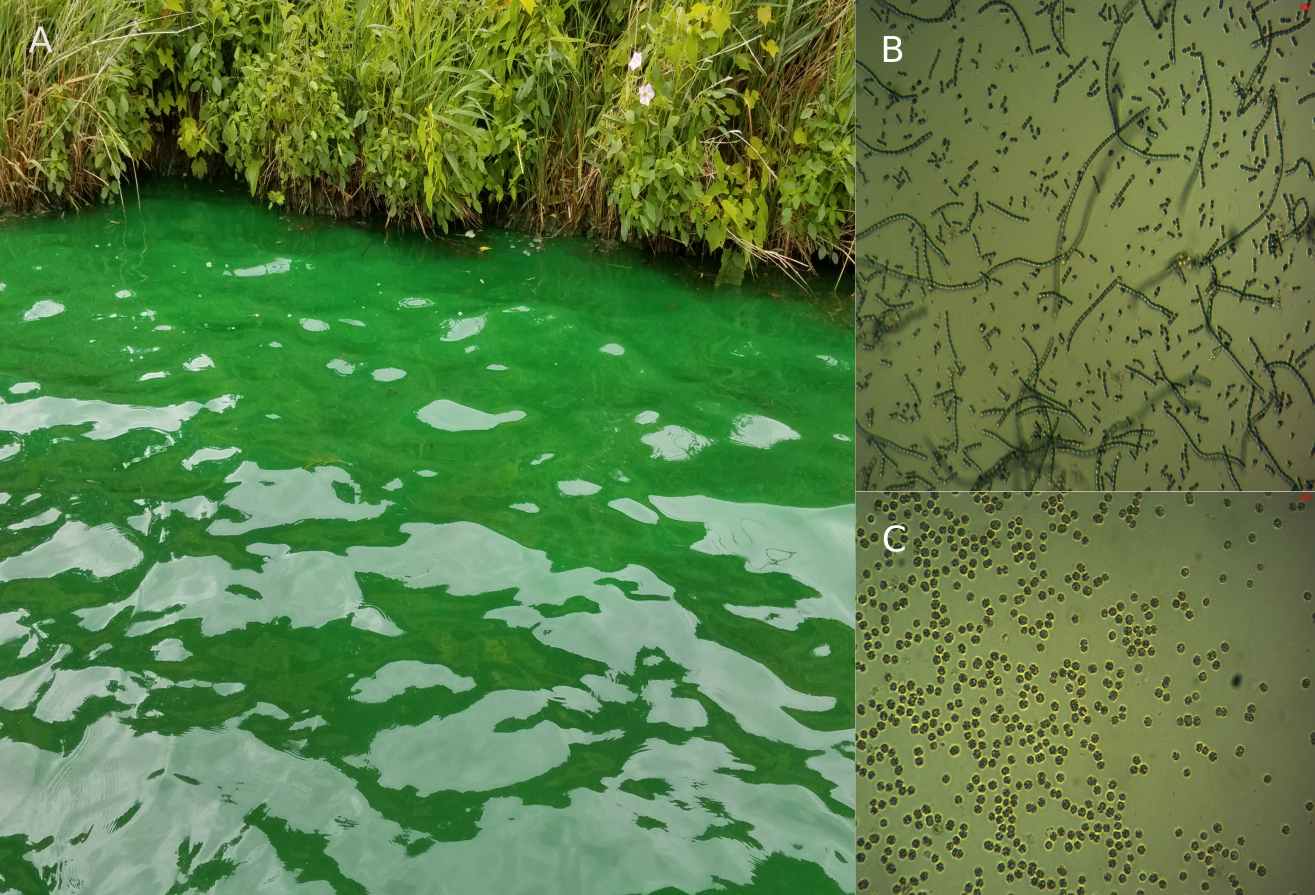
\includegraphics[width=\textwidth]{cyano.png}
	\caption{
		Examples of Harmful Algal Blooms. (A): A bloom in Manitou Lake. Picture taken by Fred Farcus. (B): Anabaena (C): Microcystis
	}
	\label{fig:cyano}
\end{figure}


\begin{figure}[!h]
   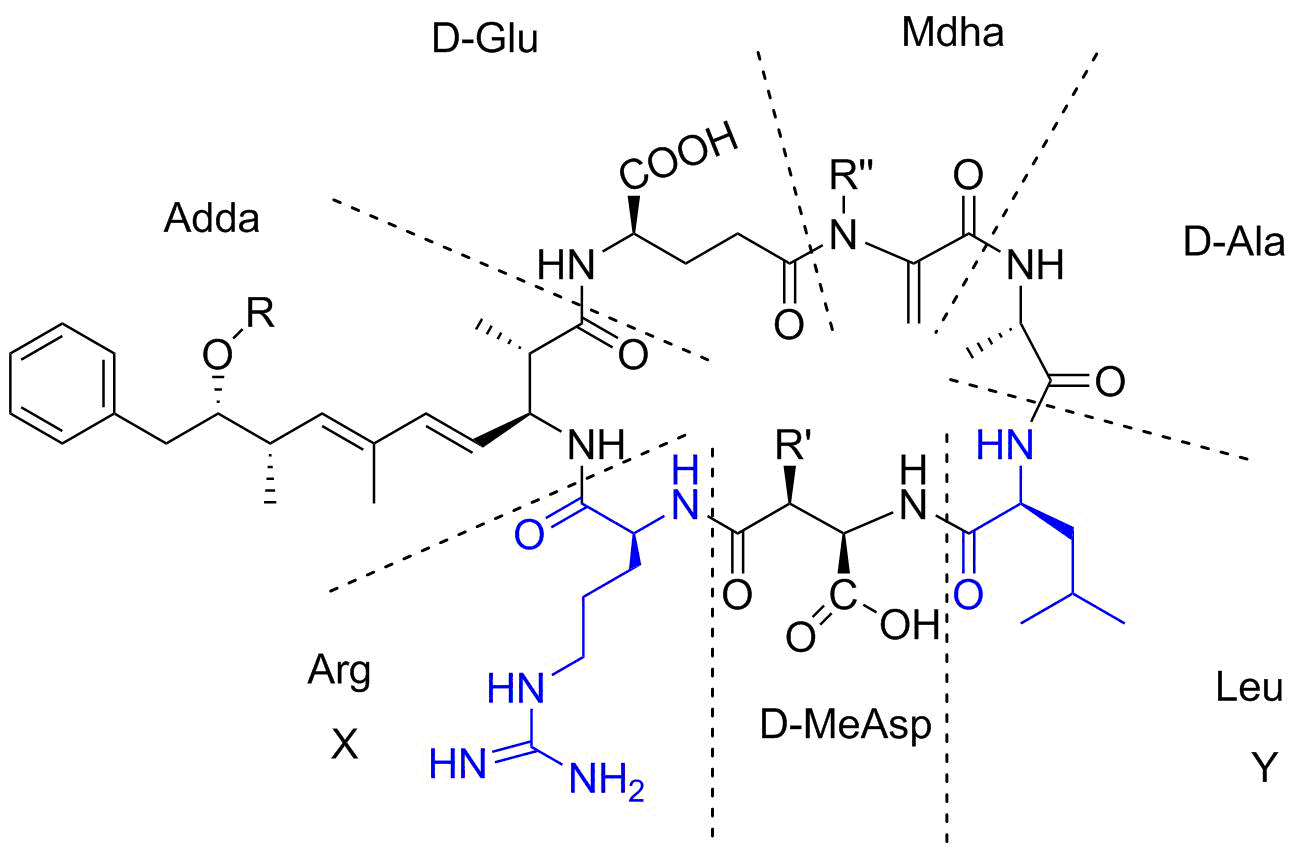
\includegraphics[width=\textwidth]{Microcystin-LR.png}
   \caption{Structure of MC-LR}
   \label{fig:structure1}
   \begin{flushleft}
   The most common structure of microcystin. The seven major moieties are separated by dashed lines. Position X and Y can be interchangeable with other variable amino acids. R and R'' can also be found demethylated in other congeners. 
     \end{flushleft}
 \end{figure}

 \clearpage

% Damages
Swimming or contact in any waterbody with \gls{hab} can pose a health risk as all \gls{hab} are irritants and some can have toxin producing species. Many of the species that are producing hepatotoxins and neurotoxins in high amounts can kill livestock, pets and wildlife \cite{anderson_harmful_2002}. The possible route of exposure  for humans can be from dermal contact, accidental ingestion, breathing in lake spray aerosols and failure of purification in drinking water plants \cite{may_aerosol_2018,codd_cyanobacterial_1999}. As stated, exposure through dermal contact can be an irritant. \gls{hab} can create lipopolysaccharide, an endotoxin, which create rashes after skin contact as it triggers a inflammatory response \cite{ moore_richard_cyanobacterial_1993}.

% Treatment
Ingestion is the most dangerous route of exposure for any cyanotoxins. Usually, complete immersion and prolonged exposure to affected waters increases the chance of ingestion of water with significant levels of cyanotoxins. Although the case is rare for humans, this is more dangerous to animals and pets \cite{koreiviene_cyanotoxin_2014}. Cyanotoxins can also be consumed in fish and wildlife that has drank enough amounts where it can bioaccumulate in their fatty tissues, eventually leading to ingestion by humans \cite{saoudi_management_2017}. Drinking water from an affected lake could  lead to acute toxicity or other symptoms \cite{monks_potent_2007}. Unfortunately, \gls{hab} can be found in storage reservoirs and source waters in regions that do not have sophisticated drinking water facilities in providing clean water. 

In addressing the removal of toxins, a water treatment facility needs to understand where most of the toxins resides.Cyanotoxins are mostly intracellular, except for the case of cylindrospermonspin \cite{rastogi_cyanotoxin-microcystins:_2014}.
With a health risk management plan, an analysis of water input (raw water) needs to identify the genera and the toxins levels intracellular and extracellular concentrations \cite{saoudi_management_2017}. The information of whether the toxin is intact within the cell or not can suggest different treatments. Intact cells should be removed as much as possible at the intake without cell lysis \cite{westrick_review_2010}. Different treatment can be used with ozone, chlorination, activated carbon and advance oxidation process \cite{koreiviene_cyanotoxin_2014, westrick_cyanotoxin_2018}. However ozone and chlorination carries risk of cell lysis and disinfection by-products. The destruction of \gls{mc} by ultraviolet radiation coupled with \ch{H2O2} is proven to be an effective treatment method \cite{he_efficient_2012}. The use of activated carbon or membrane filteration is effective but costly to implement as a routine \cite{koreiviene_cyanotoxin_2014}. Removal of toxins can be treated by oxidants such as \ch{KMnO4} which oxidizes the dissolved toxins and prevent the cells to lyse \cite{westrick_cyanotoxin_2018}. An effective health risk managment plan would implement a multipoint check system in the water treatment process and also be economically viable \cite{westrick_review_2010,saoudi_management_2017}.

\section{Environmental Drivers of Harmful Algal Blooms}
% Drivers
Cyanobacteria in it's natural environment is complex and often unexpected. The mechanism for what drives the proliferation is not fully understood as some studies have attempted to explain what factors are responsible of their explosive growth \cite{dittmann_cyanobacterial_2012, noauthor_human_2012}. As autotrophs, cyanobacteria rely on sunlight for their energy. \gls{hab} can rapidly grow under warm, sunny and nutrient-rich conditions \cite{rastogi_cyanotoxin-microcystins:_2014}. \gls{hab} are most likely to occur in the summer or warmer months where primary productivity is most likely to peak due to increase daylight, warmer temperature and low water flow in streams and rivers \cite{vannote_river_1980,chapra_climate_2017-2}.
% Some cyanos are nitrogen fixators, succession of nitrogen to microcystin..etc
Excess nutrients is long believed to significantly impact the growth of \gls{hab} \cite{anderson_harmful_2002,anderson_harmful_2002}. Aside from light, nutrients such as soluble phosphorus and nitrogen can be limiting factors in growth \cite{tilman_phytoplankton_1982}. However, the relationship is not as clear as some expect. Urbanization and agriculture can produce excess nutrient runoff, creating a rich environment in lakes and coastal environments which can thrive \gls{hab} growth, often regarded as cultural eutrophication\cite{smith_eutrophication_2009}.  Organic and inorganic forms of nutrients  usually are from non-point sources such as septic tanks, animal waste and agricultural runoff. Phosphorus is the main culprit in freshwater in causing \gls{hab} \cite{anderson_harmful_2002}. For the bloom in Lake Erie, some studies suggests the nutrient runnoff into the  Maumee river, which has and its watershed mostly comprised of agriculture \cite{michalak_record-setting_2013, chaffin_accuracy_2018}. Other studies in other areas worldwide, similar to Lake Erie, have shown nutrient enrich conditions usually from agricultural runoff or disturbance of ecological conditions that impacts nutrient cycle to cause blooms \cite{ahn_evaluation_2011, ahn_rainfall_2002, anderson_harmful_2002, jiang_statistical_2008}.

Ecological factors could be a major factor in some cases. Previous studies in inland Michigan lakes are finding \emph{Dreissena polymorpha} (zebra mussels) to have an impact on finding blooms \cite{vanderploeg_zebra_2001}. In a study done by Michigan State University \cite{raikow_dominance_2004} found zebra mussels can promote phytoplankton growth due to their effect on bloom ecology. Some studies suggests that of zebra mussels should be incorporated in building a predictive model as they have a significant impact on \gls{hab} with their presence \cite{lavrentyev_effects_1995, knoll_invasive_2008, raikow_dominance_2004}. In our survey, we will investigate whether zebra mussels have an influence on MC concentration or cyanobacteria population.

\section{Application of Technology}
% PREDICTIVE models
Statistical predictive models are increasingly being used to forecast \gls{hab}. Models coupled with weather data have been increasingly successful with wind direction, speed, temperature and precipitation being the best predictor of \gls{hab}. Along coastal environment,   \gls{noaa} uses real-time data from satellite to predict \gls{hab} on the Gulf of Mexico, Lake Erie, and other coastal environments based on satellite data and weather models \cite{kavanaugh_assessment_2013}. Remote sensing instruments such as buoys equipped with sensors have signifigantly improved, capable of collecting multiple water characteristics in real-time. In predicting \gls{hab}, fluorescence of chlorophyll-a levels can be measured continuously which can indicate growth of cyanobacteria. In addition, phycocyanin, an accessory pigment found in cyanobacteria is also an effective parameter to uniquely identify and measure the relative biomass \cite{ahn_rainfall_2002,li_semi-analytical_2012}. This data can provide more information in understanding what seems to drive their growth. Most importantly, the \gls{hab} forecast warnings can prevent exposure and improve communication with the public. They have provide comprehensive information continuously available for the public on their website \footnote{\url{https://tidesandcurrents.noaa.gov/hab_info.html}}. 

Inland lakes, satellite imagery is not ideal cloudy conditions. Forecasting for inland lakes does not work with satellite imagery as the extent of the lake's area will often limit the predictability. An effective predictive models should be based on features that are found to contributes to \gls{hab} with measured abiotic and biotic factors. Understanding the main drivers for cyanobacteria can help to predict HAB occurrences.

One of the challenges in assessing water quality of a lake is the frequency of sampling. \gls{hab} is sporadic and often can be missed if sampling regime is too sparse. Monitoring for \gls{hab} requires frequent sampling regime inorder to not to miss a  \gls{hab} events. Concentrations of cyanotoxins may fluctuate through time and sampling at a large interval may not capture the reality of the lake's condition. 

\gls{spatts} is a unique method of monitoring waterbodies in a more time-integrative approach. A porous bag or a sachet is filled with a resin inside a permeable bag.
SPATT is used in for monitoring other analyte of interest such as diarrhetic shellfish poisoning \cite{mackenzie_solid_2004}. %%%%%%%%%%%%NEED MORE CITATION$$$$$$$$
The SPATT bag  is submerged in a waterbody of interest for a period of time. During this period, free-floating compounds will adsorb onto the polymer beads.  SPATT can are then retrieved and analyzed for chemical analytes of interest. This technique can be useful if sampling frequency is financially limited.



 \section{Goals and Aims}
% TODO reread this and expand it
My goal is to explore what drives HAB development and build a predictive model based from our collected data.  With the collected observations, I investigated the best possible predictive model from our dataset. Eventually with the built model based on each lake's unique geological characteristics and be ranked by the likelihood of \gls{hab}.
Some studies build predictive models based using cyanobacterial cell count or mass, concentrations of chlorophyll-a and MC concentrations as a response variable as its most likely associated with \gls{hab} \cite{moore_richard_cyanobacterial_1993, ahn_evaluation_2011, jiang_statistical_2008, beaulieu_nutrients_2013, taranu_predicting_2017}.
%Cyanobacteria cell counts would be ideal to measure whether the lake is exhibiting a bloom.
The total MC concentration measured by \gls{lcmsms} was used as the main predictor variable of interest. The \emph{16s rRNA} gene copies measured by \gls{qpcr} was also observed as a response variables as well as this measures relatively amount cyanobacteria. In our survey on 29 inland lakes in Michigan, we seek to understand what drives \gls{hab} and build a predictive model on \gls{mc}. In addition, we also analyzed for cylindrospermopsin and anatoxin in our surveyed lakes. Before the survey, I hypothesized if the lake's watershed is more urbanized areas, I would expect higher MC concentrations. Developed land can increase nutrient runoff which can increase algal blooms. Previous studies have shown developed areas as having a major influence on the occurrence of \gls{hab} because of more possible sources like applied fertilizer or leaky septic tanks \cite{beaver_land_2014, anderson_harmful_2002}. Lakes with higher developed areas may also have a possible influence nutrient mobility, which in turn drive MC production. I expect this relationship to also be similar with total cyanobacteria measured by \gls{qpcr}, chloraphyl, \emph{mcyE}. % Must put in that I analyzed for chloraphyll, phyco, and mcyE.  

With the extent of the study, I would expect to find some key features that can reveal a definite pattern which can describe what drives \gls{hab}. Prior to the study, I hypothesized lakes with dominant urbanization would see an increase in \gls{mc} concentrations. In addition, I also would expect the presence of Zebra mussels to have a positive influence as well. My research objectives:

\begin{enumerate}
 \item Harmful algal blooms are influenced by  developed/urban land, which can be used to predict MC concentrations
 \item Lakes with the presence of zebra mussel will have a higher concentration of MC than lakes with none found.
 \item Nutrient concentrations can be explained by land use characteristics
 \item Identify important features that influence \gls{hab}.

\end{enumerate}

\chapter{SURVEY DESIGN AND METHODS}

\section{Survey Study of Michigan Inland Lakes} 
As a grantee of \gls{mdeq}, our main objective is to develop a predictive model. We address the challenge by assessing land use information and collected cyanotoxin data and investigate statistical relationship that potentially drives \gls{hab}. For the summer of 2017, a total of 29 inland lakes were sampled. Prior to sampling, permission of riparian owner was obtained for lakes which did not have public access. Sample surveying began in the month of June 2017 until October 2017. Each month, every lake one was sampled once. Sampling locations were chosen from known list of lakes reported with \gls{hab} given by Aaron Parker from \gls{mdeq} and existing collaborative partners with different lake associations. In addition, we also chose lakes that are reasonably close to I-75 expressway for the ease of transportation. See figure \ref{fig:overview} for a map of our lakes sites and for more detail, see table \ref{tab:Surveyed Lakes}.

Cyanotoxins were analyzed primarily by \gls{lcmsms}. For \gls{mc}, 12 different congeners along with nodularin were identified and quantified by \gls{lcmsms}. Total \gls{mc} analyzed by \gls{lcmsms} is the sum of the 12 congeners and nodularin measured in the sample. In parallel, \gls{elisa} was used to quantify total \gls{mc} and nodularins.  we compared the results of total \gls{mc} from both \gls{lcmsms} and \gls{elisa} and assessed the agreement between the two. Cylindrospermopsin and Anatoxin-a were also analyzed with \gls{lcmsms}. In addition, we also used \gls{qpcr} which detects and quantifies \emph{16s rRNA}, \emph{mcyE/nadF}, \emph{sxtA}, and \emph{cyrA} gene. The \emph{16s rRNA} gene is a common gene in \gls{qpcr} to uniquely identify bacterial phylogeny and taxonomy \cite{janda_16s_2007}.  The \emph{mcyE/nadF}, \emph{sxtA} and \emph{cyrA} are gene clusters responsible of synthesizing \gls{mc}, nodularin, saxitoxin-a and cylindrospermonsin. A commercial kit from Phytoxigene Inc. \footnote{Diagnostic Technology, 7 Narabang Way, Belrose 2085. Australia.} contained the primers and probes neccessary for \gls{qpcr}.  

In our survey we analyzed different water parameters that could lead us to understand key drivers of \gls{hab}. Upon arrival at each lake pH, conductance, dissolved oxygen and lake water temprature. A nephelometer was used to measure turbidity as well. A portable fluorometer was used to measure chloraphyll-a and phycocyanin emmission. Dissolved nitrate+nitrite, orthophosphate, ammonia were analyzed colorimetrically on the collected water samples. In addition, total phosphorus and total nitrogen was also analyzed with collected water samples. Land use for each lake's watershed was calculated using \gls{gis} software. Data was compiled for statistical analysis.

\begin{figure}[!h]
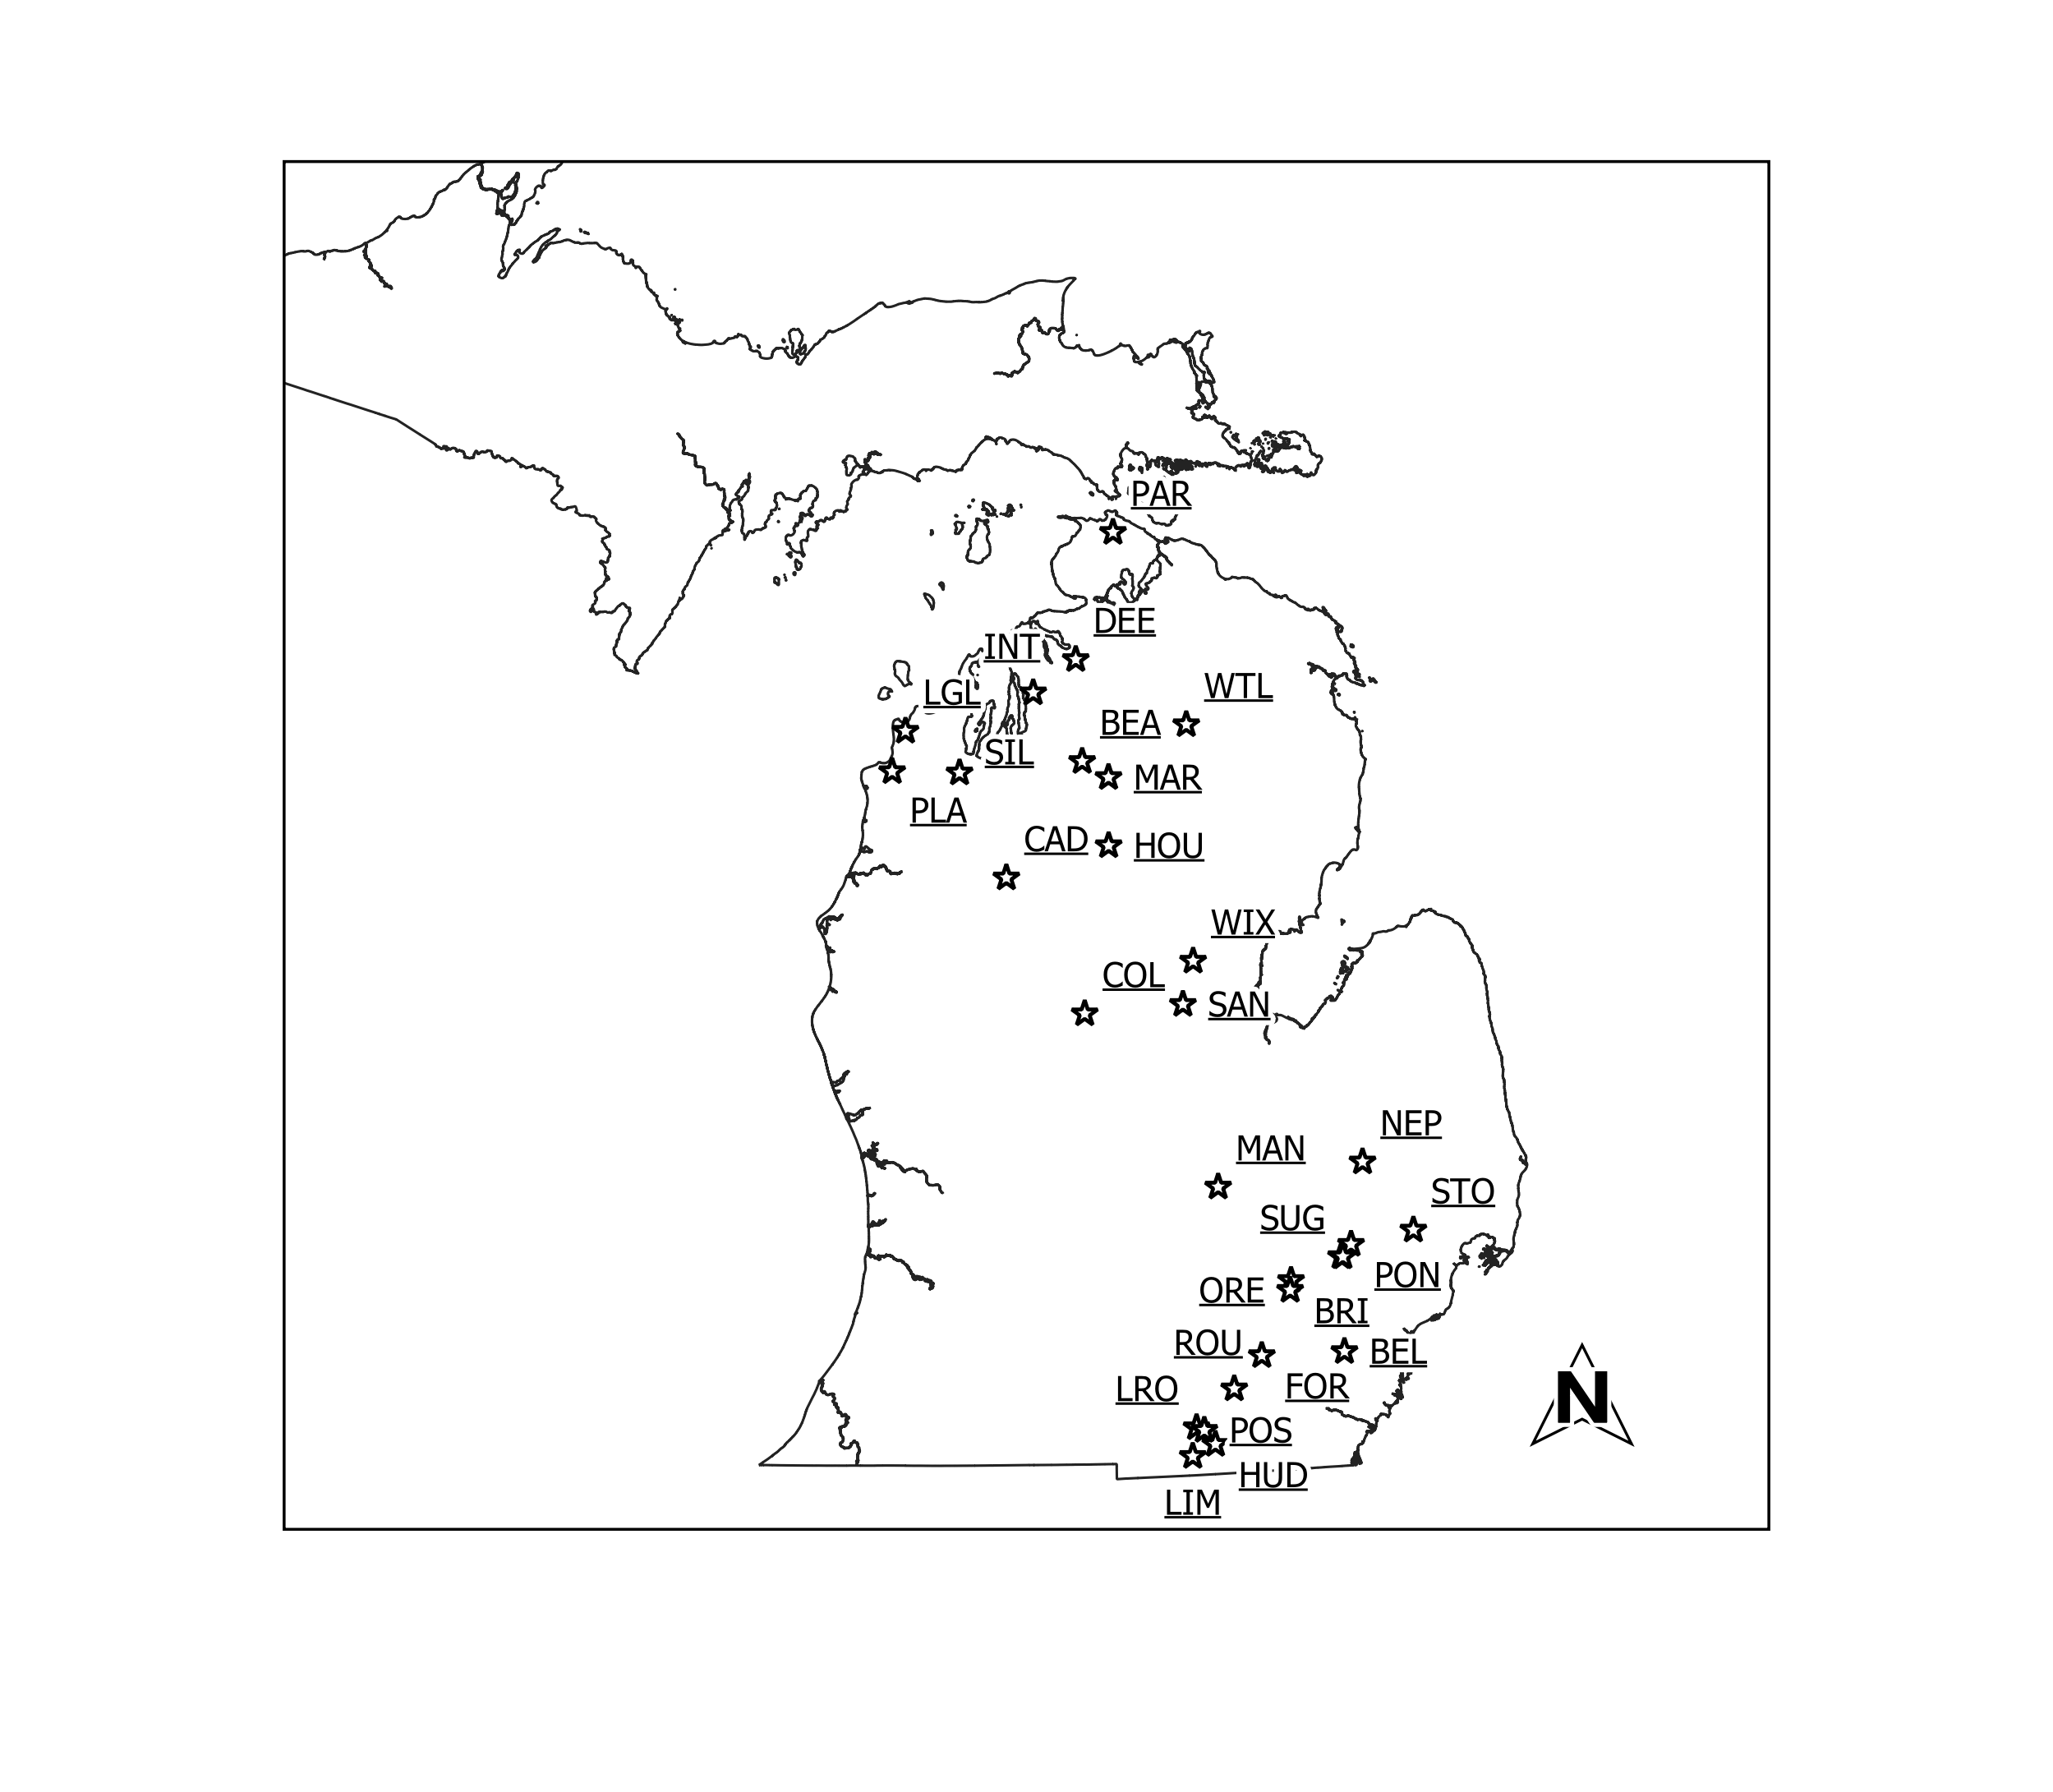
\includegraphics[width=\textwidth]{figures/Overview}
\caption{Map of Sampled Lake Sites in Michigan}
\label{fig:overview}
\end{figure}

\clearpage
\subsection{Water Grab Sampling} \label{sampling}

Water samples were collected by wading in toward the center of the lake until water height reached waist height. All water grab samples were taken roughly one foot below water surface. Each water collecting vessel was rinsed 3 times with the lake water before obtaining final sample. A total of 4 team of field surveyors sampled each with designated lakes. At each lake, a hand-held multi-meter was used to measure pH, conductivity ($\mu$S/cm), dissolved oxygen (mg/L) and temperature ($^\circ$C). Phycocyanin and chlorophyll fluorescence were also measured using an portable fluorometer by Amiscience with the optical excitation of 470 nm and 590 nm and the emission is read at 685 nm, which is measured in \gls{rfu}. Each fluorometer for each surveyor was calibrated against rhodamine WT\footnote{Sodium chloride 4-[3,6-bis(diethylamino)-9-xantheniumyl]isophthalate (2:1:1)} dye as a secondary calibration standard, which ensured the calibration is relative to other fluorometer and to prevent drift. A portable meter from Hach was used to measure turbidity in \gls{ntu}. Formazin standards were used to calibrate the turbidity meter.

In July 2017, a constructed sampler float was installed at each lake. The sampler was constructed by the Dr. Raffel's team, which consisted of 3 plexi-glass plates and placed at each sampling location for the purpose of collecting zebra mussels (see figure \ref{fig:samplerr}). The stack of three square plexiglass sheets were about 15cm,20cm, and 25cm in diameter which gives them a total surface area of 0.23 m$^2$ per sampler. In addition, also installed a slotted PVC pipe which contains a \gls{spatts}, a beta test of a new method of monitoring toxins. This method will be disscussed in chapter \ref{ch:spattss}. A majority of samplers were installed on the riparian owner's dock, or as a float. HOBO Pendant\texttrademark temperature and light logger were installed on floats at each lake site. In October, we collected the samplers and scraped all mussels into a glass mason jar for analysis of biomass.

Water sampling kits were prepared by storing pre-labeled water vessels in zip-lock bags for each lake to prevent cross-contamination between different lake water samples during sampling transport and storage. Each sampling kit contained 60mL \gls{petg} vials for MC analysis, 100mL sterile IDEXX bottles for QPCR analysis, 50mL polypropylene centrifuge vials and 250 mL \gls{hpde} Nalgene bottles for nutrient analysis. Each kit also provided alkaline Lugol's iodine solution for preserving cyanobacteria samples for identification and 3M \ch{H2SO4} for acid preservation of nutrient samples. The 3M \ch{H2SO4} is in a separate zip-lock bag with roughly 20g of \ch{NaCO3} wrapped in paper towel to neutralize the sulfuric acid incase of a spill or a leak. Lugol's iodine solution was prepared by dissolving 100g of \ch{KI}, 100g of \ch{I2} and 100g of sodium acetate dissolved in 1 liter of water. See figure \ref{fig:samplekit} for an example of a sampling kit.

\begin{figure}[!h]
\centering
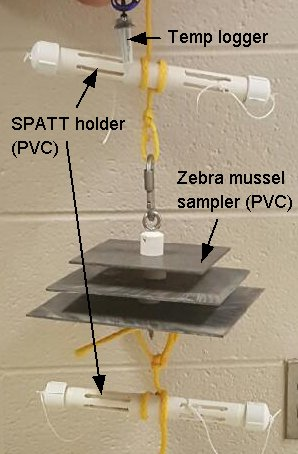
\includegraphics[width=\textwidth, height=18cm]{figures/samplers}
\caption{Picture of the constructed sampler installed at each lake. HOBO Pendant is attached with a secure carabiner. SPATT PVC holders and Zebra mussel sampler is shown }
\label{fig:samplerr}
\end{figure}

\begin{figure}[!h]
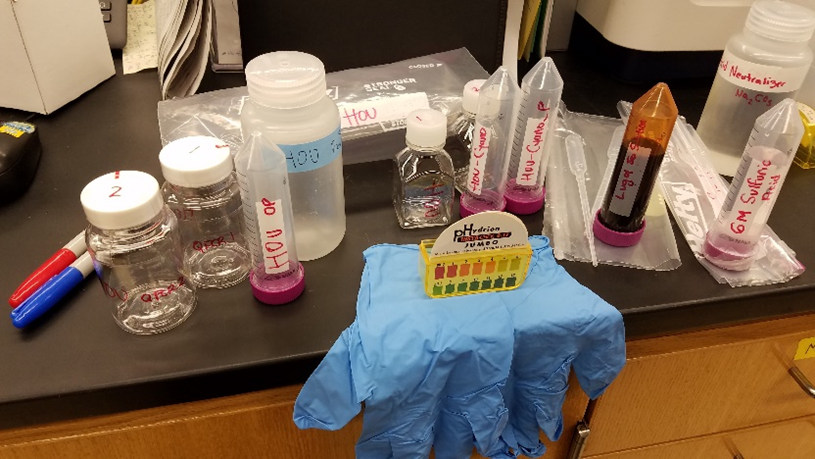
\includegraphics[width=\textwidth]{figures/samplekit}
\caption{An example of sampling kit and the contents}
\label{fig:samplekit}
\end{figure}

\clearpage
\newpage

\subsection{Solid Phase Adsorption Toxin Tracking}

One of the challenges in assessing water quality of a lake is the frequency of sampling. \gls{hab} is sporadic and often can be missed if sampling regime is too sparse. Monitoring for \gls{hab} requires more frequent visits to sample inorder to not to miss a  \gls{hab} events. Concentrations may fluctuate through time and sampling at a large interval may not capture the reality of the lake's condition. 

Solid Phase Adsorption Toxin Tracking (SPATT) is new unique method of monitoring waterbodies in a more time-integrative approach. SPATT is used as a bag or a sachet is filled with a porous resin inside a permeable bag.
SPATT is used in for monitoring other analyte of interest such as diarrhetic shellfish poisoning \cite{mackenzie_solid_2004}. %%%%%%%%%%%%NEED MORE CITATION$$$$$$$$
The SPATT bag  is submerged in a waterbody of interest for a period of time. During this period, free-floating compounds will adsorb onto the polymer beads.  SPATT can are then retrieved and analyzed for chemical analytes of interest. This technique can be useful if sampling frequency is financially limited.

In addition in our survey, we assessed the efficacy of this new technique. 


The SPATT bag will be make with Nitex\footnote{Purchased from Dynamic Aqua-Supply Ltd.  \url{http://www.dynamicaqua.com/nitex.html}} and filled with HP-20\footnote{Purchased from Sigma Aldrich: CAS Number 9052-95-3}, a non-polar resin (styrene-divinylbenzene copolymer),
To construct the SPATT bags, a 1 meter x 5 centimeter strip of Nitex mesh were cut with sharp blade. The Nitex strip was sewn by folding half length-wise (or \emph{hot dog} style). With tape holding the fold, the end of the strip was sewn 0.5cm from the edge. Stitching design was tight to ensure no leakage of polymer beads.

9-10cm of sewn Nitex strips were cut and zip-tied about 0.5cm at one end. 3.00-3.01 grams of HP-20 resin was filled using a funnel. The other end is zip-tied once the Nitex bag is full. SPATT bags are activated by soaking in 100\% methanol for 24 hours under $4^\circ$C. Next the SPATTs were rinsed with Milli-Q water and then soaked for 24 hours in Milli-Q water under $4^\circ$C before deploying the SPATT bag in our target sample lakes.

At each lake site, two SPATT bags were loaded into a slotted PVC pipe. At each lake, a float was installed as described in section \ref{sampling}. SPATT are left for about a month at each lake. When SPATT are retrieved, they are carefully removed and rinsed with Milli-Q water and stored in a 15mL centrifuge vial with a plastic spacer on the bottom. SPATT are stored at $4^\circ$C during transport back to the lab. The SPATT are centrifuged at 8000rpm. The spacer allows liquid to pool on the bottom when centrifuged. When centrifuged, the SPATT bags are cut open and the resin is poured into a 50mL centrifuge tube. Milli-Q water is used to rinse the SPATT bags to effectively transfer all the resin. About 30mL of Milli-Q water is used. The solution is allowed to rest so the resin settles to the bottom. Using a pipet, the water is carefully decanted until the total volume is 5mL.  A solution of 80\% methanol with 10$\mu$M ammonium formate is added to the tube until the total volume is 45mL. The solution is gently mixed and then allowed to settle for 30 minutes. A 3.5mL aliqout of the supernatant is transferred to glass vials and analyzed by \gls{lcmsms} by the Westerick group. Similiar to our analysis of the grab sample, the SPATT were analyzed for all 12 congeners of \gls{mc} and nodularin (see section \ref{sc:lcms}). The final reported value is calculated to give the amount of \gls{mc} per gram of resin per day. It is calculated by this equation:

\begin {center} 
$ng of MC/g of resin per day = (mg of MC)$
\end{center}

\section{Analytical Methods}
\subsection{Liquid Chromatography Mass Spectrometry} \label{sc:lcms}

The collected water samples were collected and stored in 60mL \gls{petg} vials. Within 3 days from sampling, the water samples were freeze-thawed for 3 cycles for cell lysis. Water samples are thawed slowly in a heated water bath at 37$^\circ$C, then frozen at -20$^\circ$C. Once finally thawed, an AcroPrep 96-well plate with glass fiber was used to filter the water samples. Once filtered, 3.500 ml aliquot of each sample above was transferred to glass vials suitable for the Thermo Scientific EQuan MAX (online sample concentrator). The samples were transported to Wayne State University and analyzed for 12 MC congeners, nodularin, anatoxin-a and cylindrospermopsin.  The Westrick group at the WSU Lumigen Instrument Center has developed a high-throughput \gls{lcmsms} analysis for \gls{mc} in surface and drinking water analyses.
The analysis done by the Westrick group's LC-MS/MS platform includes a Thermo Scientific EQuan MAX (online sample concentrator) and ThermoFisher’s UltiMate 3000 \gls{uhplc} system and a \gls{tsq} Quantiva.
Their method is similar to EPA method 544 with the addition of 5 more congener analytes \cite{shoemaker_method_2015}. Figure \ref{fig:spectra} shows a standard chromatogram of all 12 \gls{mc}, nodularin, and the ethylated internal standard (\ch{[C_2D_5]} MC-LR) eluting between 2.2 and 5.2 minutes allowing for the total analyses time to be less than 12 minutes.  The \gls{mdl} is 0.030  $\mu$g/L  for all cyantoxin analysis. 

\begin{figure}[!h]
\centering
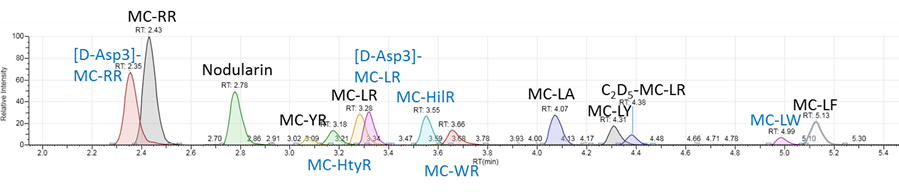
\includegraphics{LCMS_CONGENERS}
\caption{Liquid chromotography-mass spectrometry chromatogram of the MC congeners. Chromatogram provided by Westrick Group}
\label{fig:spectra}
\end{figure}

\clearpage

\subsection{Enzyme-Linked Immunosorbant Assay}

A commercial Microcystin/Nodularins ADDA ELISA kit was used from Abraxis to analyze total microcystin\footnote{https://www.abraxiskits.com/products/algal-toxins/}. The analysis uses a polyclonal antibody which specifically binds to the ADDA moiety found in MC. However it does not distinguish between different congeners and the given results are in terms of MC-LR equivalance. The analysis followed the reccommended guidelines provided by the EPA \cite{usepa_method_2016}. In preperation of loading the plate,  100$\mu$L of standards, controls, blanks and samples are aliquoted into a seperate sterile 96-well plate. To minimize assay drift caused by slow plate loading, a multi-channel pipettor was used to load the the standards, controls, blanks and samples to the final 96-well plate. The assay procedures were carried out and read by Synergy H1 microplate reader from Biotek.

\subsection{Quantitative Polymerase Chain Reaction}

Phytoxigene\texttrademark  CyanoDTec cyanobacteria and toxin test kit was preformed with Applied Biosystem StepOnePlus\texttrademark \gls{qpcr}. The kit provides two separate assay mixes. Total cyanobacteria assay will quantify the 16srRNA gene copies found in the water sample. Both the total cyanobacteria and toxin gene assay  were analyzed in parallel for each month of grab samples. The primer/probe sequence is unknown.  The PCR reaction mix contained 5 $\mu$L of template/sample extracts and 20 $\mu$L of rehydrated mastermix.  Each sample were run in singlicate due to limited resources. Positive standards for target genes  were run on each PCR analysis. Phytoxigene\texttrademark  CyanoNAS nucleic standards were used to generate standard curves for quantification of gene copies. The CyanoNAS was removed from -20$^\circ$C and allowed to thaw prior to analysis.  Standards were run in duplicates.

Samples for QPCR were filtered either on site with portable Santino pump, or brought back to the lab for filtration within 8 hours from sampling.
At each lake, 100mL or more of water sample was collected in a sterile IDEXX vessel then filtered through a 0.4$\mu$m pore size polycarbonate membrane  and stored at -20$^\circ$C until QPCR. Once filtered, they are immediately transferred into BioGX vials. BioGX vials are stored at -80$^\circ$C until analysis. BioGx vials contains 500 uL of lysis buffer, lysis beads and filtrate. For cell lysis, vials were vigorously shaken by bead beater on the highest setting for 2 minutes. After bead beaten, sample vials were centrifuged for 1 min. After centrifuge, 50 $\mu$L of the supernatant was transferred to a microcentrifuge tube and centrifuged for 5 min, then roughly 25 $\mu$L of the final supernatant to another set of microcentrifuge tubes for PCR template.  Sample extracts are stored at 4$^\circ$C and analyzed within 4 hours.

From following the recommended guide by Phytoxigene, the PCR heat cycles were programmed with initial denaturing step at 95$^\circ$C for 2 min, then a repeating of 95$^\circ$C for 15 seconds and 60$^\circ$C for 30 seconds reaching a total of 40 cycles. The appropriate gene target filters were manually set to match the emission spectra of each probe.  For each PCR run, a standard curve was generated  from within the StepOnePlus software. CT threshold and baseline were manually assigned for each run by visually assessing each target run. The calculated gene copies are done automatically by the StepOnePlus software, expressed in gene copies/$\mu$L of lysate. The final reportable value is calculated by this equation:

\begin{center}
  $Genecopies/mL = (Genecopies/\mu L \: of \: lysate) \times (\frac{500\mu L \: of \: lysate}{\text{mL of Sample Volume}})$
\end{center}

\subsection{Nutrients}

Two 125-mL \gls{hpde} Nalgene bottles were used to collect acid-preserved water samples with 2 mL of 3M \ch{H2SO4}, resulting to pH \textless 2. A 50-mL centrifuge tube is used to collect water samples without acid preservation for orthophosphate. One of the two Nalgene bottles is allocated for ammonia-N and nitrate+nitrite-N by our lab at Oakland University, and the other is for total phosphorus and total nitrogen run by Ben Southwell and his team at Lake Superior State University.  Samples were kept  at 4 $^\circ$C during transport and stored at -20$^\circ$C. Upon receiving samples from field samplers samples are thawed if frozen and cool at 4$^\circ$C. All lake water samples were homogenized by inverting 8 times and aliquoted into 15-mL centrifuge vials and centrifuged at 3000rpm for 45 seconds. The supernatant was collected into a clean 3-mL vial to be prepared for the AQ1 auto sampler. All samples were analyzed within the appropriate time frame from time of sampling collection.

Nutrient concentrations are quantified by colorimetric analysis with  AQ1 from SEAL Analytical\footnote{SEAL Analytical Inc.
6501 West Donges Bay Road Mequon, Wisconsin 53092}, a discrete colorimetric analyzer.  Ammonia-N (\ch{NH3}) is quantified by a reaction with dichloroisocyanurate and dissolve ammonia to create chloramines which  forms a blue-green color with salicylate which is measured at 660 nm \cite{usepa_method_1993-2}. The range of application is between 0.02-1.0 mg N/L with a mininum detection limit of 0.006 mg N/L for quantifying ammonia.  Nitrate+nitrite-N (\ch{NO3^{-}} $+$ \ch{NO2^{-}}) is analyzed with an open tube copperized cadmium coil which the pH buffered sample water will have nitrate reduced to nitrite. The reduced water sample is then reacts with sulfanilamide with the presence of $N$-(1-napthyl)-ethylenediamine dihydrochloride to form a reddish color measured at 520 nm \cite{usepa_method_1993}. The range of application for analyzing nitrate+nitrite is between 0.25-15 mg N/L with a detection limit of 0.04 mg N/L.  Orthophosphate-P (\ch{PO4^{-3}}) is analyzed with acidic molybdate solution with antimony potassium tartrate to form a complex with dissolved orthophosphate. The complex is reduced with ascorbic acid to create a blue color measured at 880 nm \cite{usepa_method_1993-3}. The range for orthosphosphate is between 0.003-0.3 mg P/L with 0.008 mg P/L as the detection limit. Total Kjeldahl nitrogen-N (organic nitrogen) is analyzed by sample digestion with copper(II) catalyst at 380$^\circ$C. Nitrogen containing compounds such as amino acids and peptides are converted to ammonia which is then reacted with hypochorite to create chloramine, which is then reacted with salicylate at a pH of 12.6 with the presence of nitroferricyanide to form a green-blue color measured at 670 nm \cite{usepa_method_1993-1}. The range for total Kjeldahl nitrogen is between 0.2 to 4.0 mg N/L with 0.07 mg N/L as the detection limit. Total phosphorus (polyphosphates and some organic phosphorus)  is analyzed by acid-persulfate digestion which water sample with ammonium persulfate and sulfuric acid is autoclaved at 121$^\circ$C for 30 minutes which organic phosphorus is converted to orthophosphate. After digestion, orthophosphate is reacted with acidic molybdate which is reduced by ascorbic acid to create a blue color measured at 880 nm \cite{usepa_method_1993-3}. The range for total phosphorus is between 0.01-1.0 mg P/L with 0.02 mg P/L as the detection limit. 



\subsection{Geographic Information System Analysis}

Watershed delineation and calculation of land use were done using \gls{qgis} \cite{qgis_development_team_qgis_2009}.
Elevation data was downloaded in bulk by an FTP client as mosaic raster files for the state of Michigan downloaded from USGS \footnote{\url{https://earthexplorer.usgs.gov/}}.
Elevation data  prepared by using $r.fill.dir$ function from \gls{grass} which fills sinks or depressions \cite{grass_development_team_geographic_2017}. A flow accumulation raster map is generated from this command. The value of each cell designates the amount of flow based on drainage characteristics the elevation data. Visually viewing the histogram of the distribution of flow accumulation values, selecting the highest values displays will display the most probable areas the flow of water will be. The pour point is where the lake's outlet, where the water is most likely to leave. This provided visual aid in selecting the pour point of each lake. A new shapefile was created and selected each lake's pour with the visual aid of stream flow lines. Using the $r.distance$ function from GRASS, it snapped each pour point to the proper place to help the delineation step. Each lake's watershed was delineated using $r.drain$ to create a elevation model map derived from the flow accumulation raster file. The drainage raster file is then used as an input for function $r.water.outlet$ along with the coordinates of fixed pour point location, which gives the shape of each lake's watershed extent.

Land use data was downloaded from the 2006 National Land Cover Database \cite{homer_development_2004}. The land use data were classified at Anderson level-II, which has 20 different classification of land distinguishing different biomes and regions.  To simplify the land use data, the raster is reclassified into 8 Anderson level-I categories using $r.recode$ tool from GRASS. The 8 reclassified Anderson level-I classes with band ID are water (11, 12), developed (21,22,23,24), barren, (31,32,33), shrubs (41,42,43), forest(52), agriculture (71), herbaceous (81,82) and wetlands (90,95). The land use raster file was transformed into a vectorized shapefile. The shapefile was merged by union (or dissolved) by each lake's watershed, which resulted area of each land use class within each lake's watershed. This data was exported as a .csv file and prepared for statistical analysis.

Precipitation data were retrieved from the \gls{ghcn} database from \gls{noaa} \cite{menne_global_2012}. Daily precipitation data was downloaded from NOAA's FTP server \footnote{\url{ftp://ftp.ncdc.noaa.gov/pub/data/ghcn/daily/}}.  The geolocation of each rain gauge station were imported into QGIS and mapped. The distribution of the rain gauges were not uniformally distributed. Thiessen/Voronoi polygons for each station were generated and overlayed on each watershed. The area of each thiessen/voronoi polygon's intersection with the corresponding catchment is divided by the area of the lake's watershed to give a weighted value. The mean areal precipitation for each lake's watershed is calculated by taking each station's measurements and multiplying by the weighted value, then averaged together.  Ambient air temperature for each watershed is simply averaged together with their intersection of the lake's watershed. Precipitation data with each sampled lake is joined by lakes watershed. Averaged 3, 5, 7, and 30 days lagged precipitation and ambient air temperature were calculated for our analysis.

\subsection{Statistical Analysis}

Each analytical measurement was compiled and organized by each sampling event. We have data sampled from Lake Superior, Lake St. Clair and Lake Erie, however with my discussions with Dr. Szlag and Dr. Raffel, we decided to exclude them in our analysis.  Their unique geology and lake morphology does not fit our focus on inland lakes.
Data manipulation and analysis was done in Program R, a statistical computing language \cite{r_core_team_r:_2018}. The ``dplyr'' package was primarily used for data cleaning, compiling and preparation to have our dataset ready for statistical analysis \cite{wickham_dplyr:_2017}. We also used other packages with program R to for additional tools to rearrange our data matrix \cite{robinson_broom:_2018}, display our graphs\cite{wickham_ggplot2:_2009,schloerke_ggally:_2017, garnier_viridis:_2018, wei_r_2017} and create statistical summary tables \cite{leifeld_texreg:_2013,  wickham_tidyverse:_2017, zhu_kableextra:_2018, hlavac_stargazer:_2018, robinson_broom:_2018} for exploratory analysis.

The requirements for building our model using linear regression assumes the distribution of explanatory and response variables to follow a normal distribution \cite{bates_fitting_2015}. The compiled dataset contained in total of 115 observations from the 29 inland lakes.
From our collected dataset, we assessed each variable's distribution and $log10$-transformed to fit a normal distribution. In order to solve the problem of data values that are zero, we added the corresponding minimum detection limit first, then applied a log transformation. See table \ref{tab:variables} for details of which variable was transformed and the shorten variable name.

For selecting the best predictor variables, a best subset linear regression analysis was used to find good predictors that can potentially explain our response variables using the ``leaps'' package from R \cite{miller_leaps:_2017}.  Measurements from each lake is a factor that may contribute as a random effect. This can be an issue where measurements from each lake is pseudo-replicated \cite{eisenhart_assumptions_1947}. Best subset and correlation matrix analysis is done on an averaged dataset based on each lake which works around this issue.
With the best variables from the regression subset, backward step-wise regression will be preformed to further refine the best fit model. Variables will be backwardly selected by F-test using simple linear regression \cite{kenward_method_1987}. Finnaly, a linear mixed effect analysis is used to verify our best models as it allows to account the variance of each sample site without taking the average of each lake site. The predictor variables are set as fixed effects and lake site as random effects with varying intercepts. A visual inspection of the residual plots is done to check if the models deviate from homoscedasticity.  The linear mixed effect models were built on the full dataset as this accounts for the variance of each of our lake site\cite{crawley_r_2007}. The library package ``lme4'' is used for our linear mixed modeling \cite{bates_fitting_2015}. Each non-nested models are rank by the lowest \gls{bic} being our best model.





% !TEX root = main.tex
\subsection{General Trends}
% from xiao explain the peaks and variability, how they avoided overfitting, and maybe k-fold validation...maybe...
% from chaffin "accuracy of data bouy" 
% Temporal trends, peaks, which sites had the highest, variablility of each site? Trends in other variables, patterns allign? 
% Beggining of spring, lake is mixed, summer its stable, fall its mixed.
In our sampled lakes for the summer season of 2017, $log10$(MC) concentration and \emph{16s rRNA} were slighly different between each monthly sample (see figure \ref{fig:time3}). We found the MC concentrations to be the highest in the month of August with an average of 1.13 $\mu$g/L compared to 0.182, 0.357 and 0.326 $\mu$g/L for the months of July, September and October. The pattern for the concentration of \emph{16s rRNA} followed similarly, but peaking in September with an average of 6.72x$10^5$ cp/L compared to 2.37x$10^4$, 5.30x$10^5$ and 4.01x$10^5$ cp/L for July, August and October. Water temperature when measured both at the time of sampling and the HOBO loggers we observe a steady decline with each month, however, we did not observe a noticable fluctuation with light intensity (see figure \ref{fig:hobo}). With our sampling regime, we did not sample in the spring or early summer months and did not sample frequently to observe a clear temporal trend. 

% Climate and Temperature

\begin{figure}[!h]
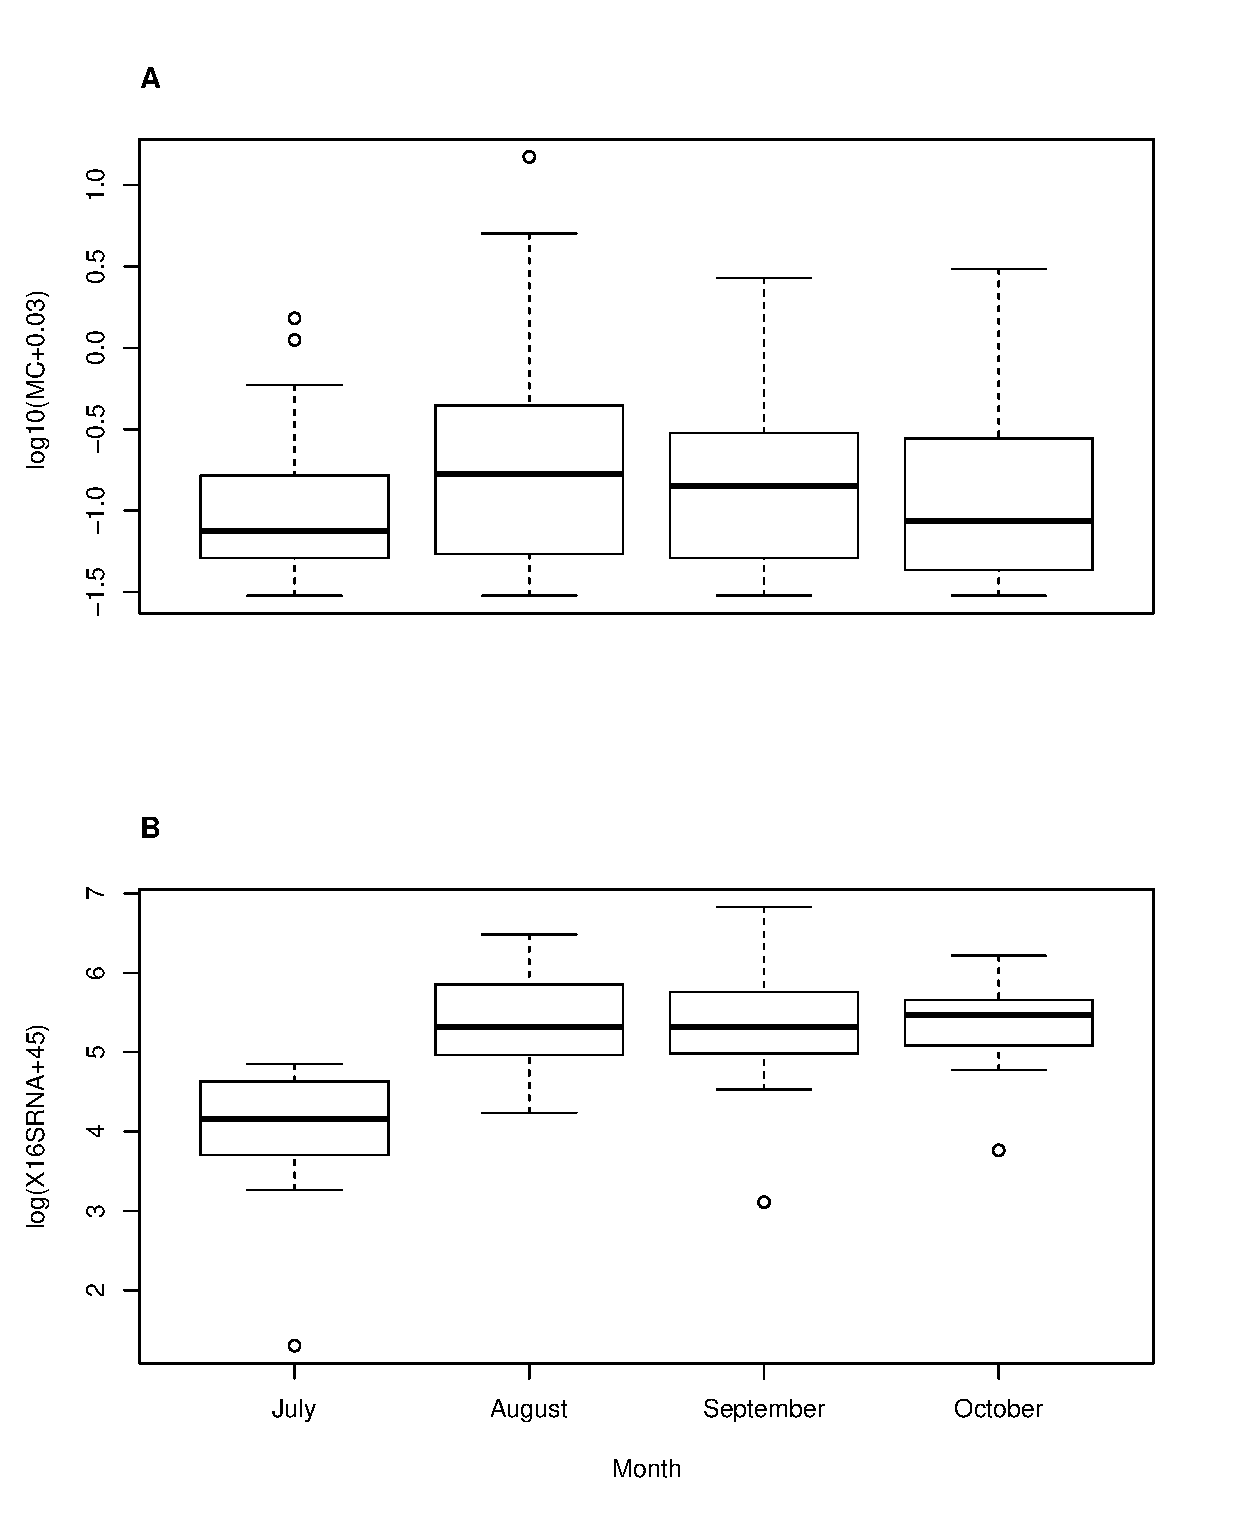
\includegraphics[width=\textwidth]{figures/time4}
\caption{
(A): Boxplot summary of the average total MC for each month. 
(B): Boxplot summary of average \emph{16s rRNA} genecopies for each month.
}
\label{fig:time3}
\end{figure}

\begin{figure}
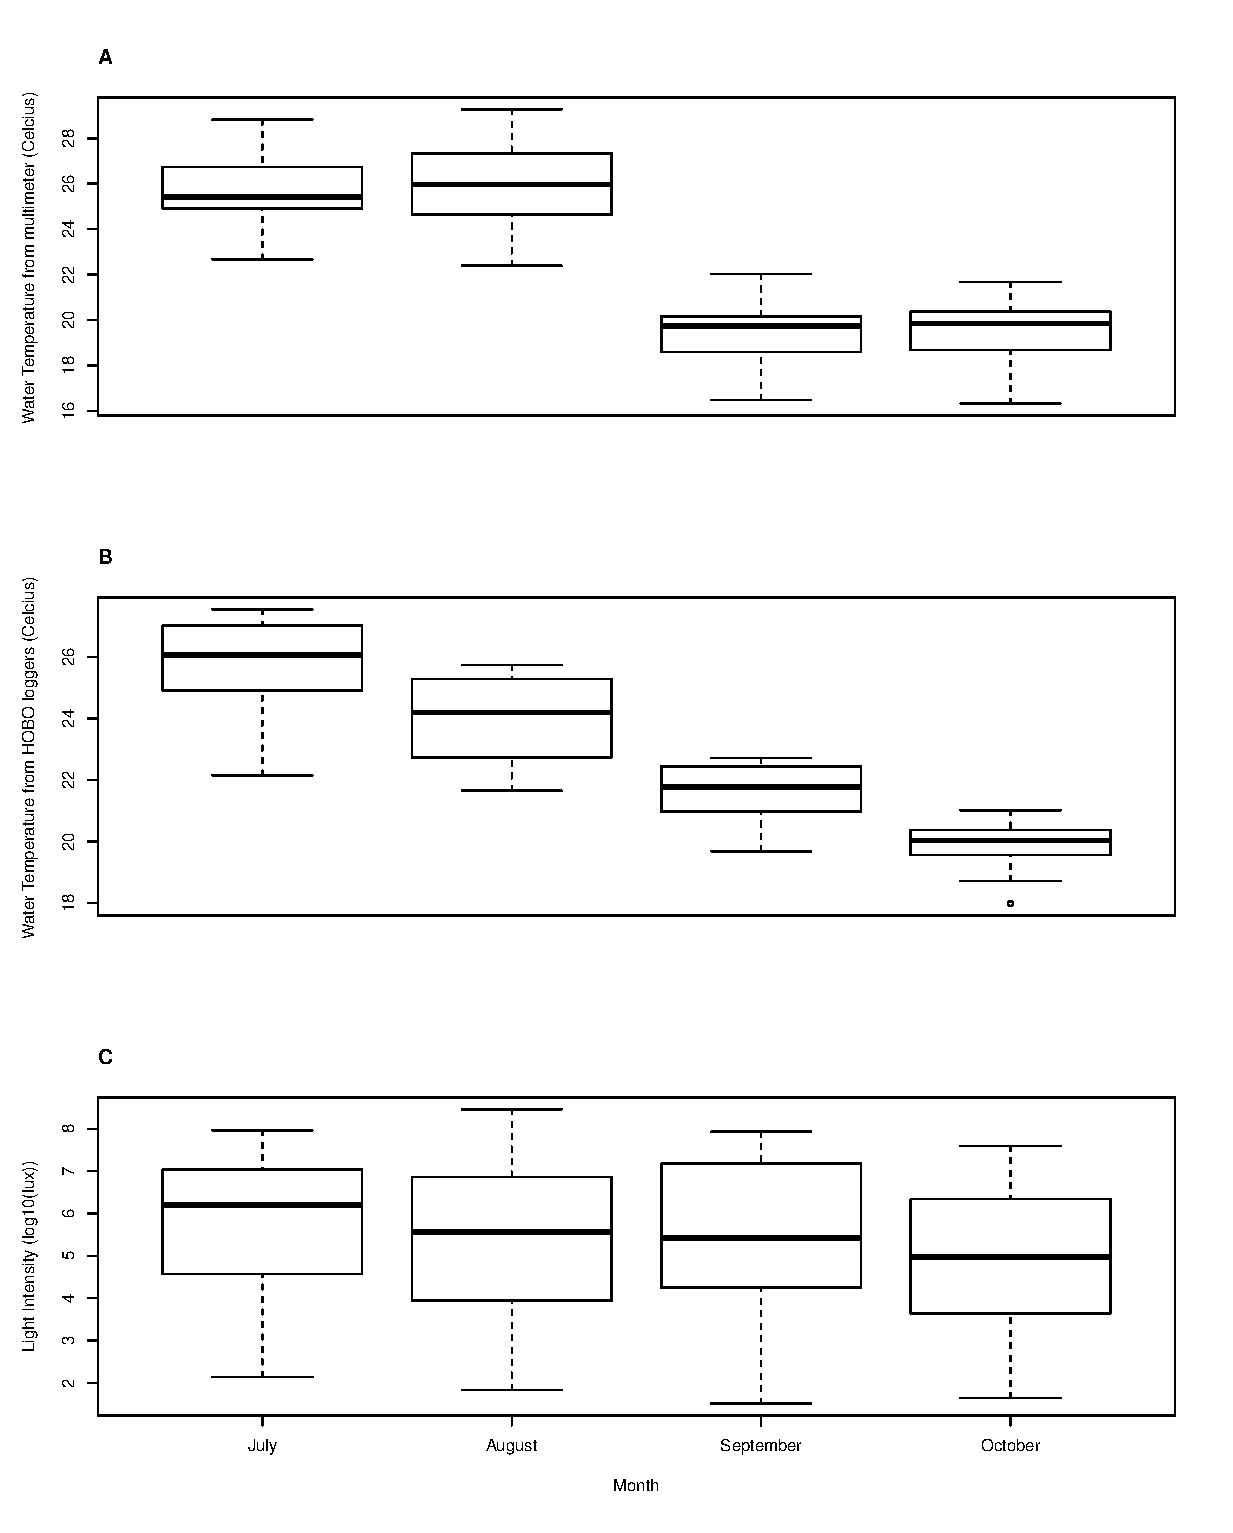
\includegraphics[width=\textwidth]{figures/hobo}
\caption{
(A): Boxplot summary of the average lake temperature measured at the time of sampling with hand-held multimeter 
(B): Boxplot summary of average lake temprature from HOBO loggers. 
(C): Boxplot summary of light intensity also measured by HOBO loggers.
} 
\label{fig:hobo}
\end{figure}

Of all the sampled lakes, we did not detect any cylindrospermonsin in our surveyed lakes. Moreover,  QPCR analysis did detect genes responsible for producing cylindrospermonsin (\emph{cyrA}) and saxitoxin (\emph{sxtA}). We detected varying amounts of \emph{mcyE} gene copies in each lake.  From the \gls{lcmsms} we found one instance of anatoxin-a detected at Brighton lake in August 2017 which was sampled during an visible bloom (2.80 $\mu$g/L of Anantoxin-a).

In our analysis of MC, MC-RR, MC-LR and MC-LA were the most detected congeners throughout the summer.  MC-RR was found with the highest concentrations 8.55 $\mu$g/L at Brighton Lake in August (see figure \ref{fig:congenerbar}).  Majority of our samples were below the EPA guidance level. From our sampled lake sites, Belleville, Brighton, Ford, Hudson, and Wixom Lake had instances of MC concentrations that exceeded the EPA guidance level of 4 $\mu$g/L both from \gls{lcmsms} and ELISA analysis (see figure \ref{fig:microcystin}).

\begin{figure}[!h]
 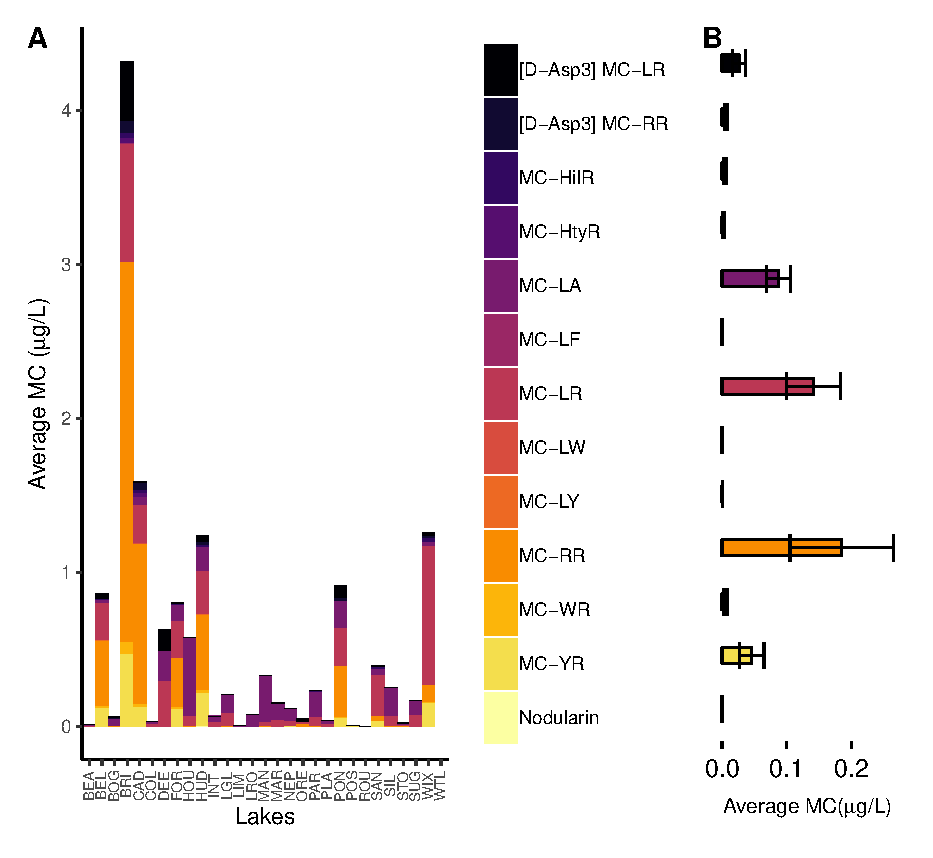
\includegraphics[width=\textwidth]{figures/congenerbar}
 \caption{
 (A): Average MC found at each lake in all four months. The height of each bar represents the total average of MC. The proportion of each congener is represented by color in each bar  
(B): Average MC congener with the included error bars represents one standard deviation of the mean}
 \label{fig:congenerbar}
\end{figure}

%EPA Graph
\begin{figure}[!h]
 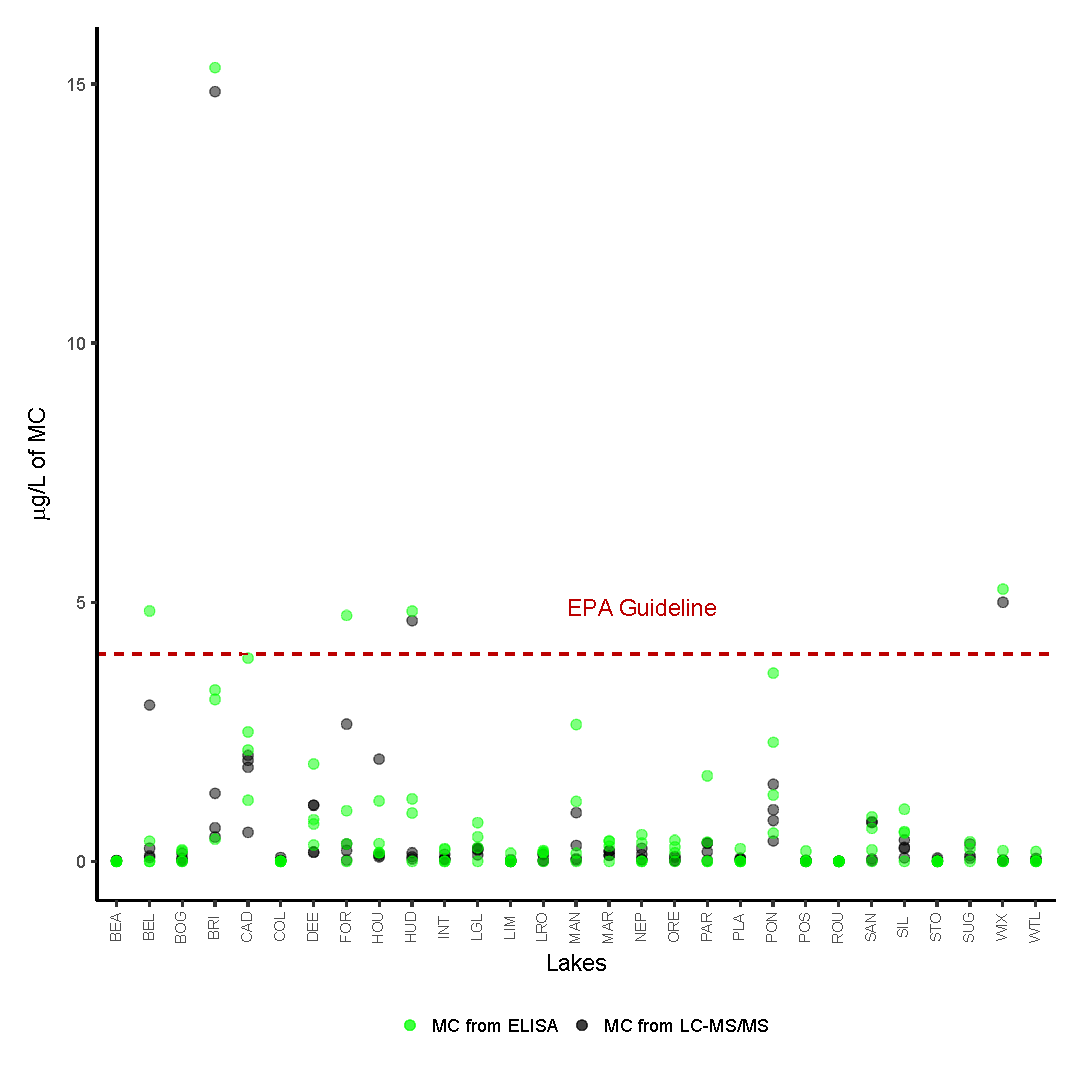
\includegraphics[width=\textwidth]{figures/Microcystin}
 \caption{Total MC with all results from ELISA and LC-MS/MS plotted by each lake}
 \label{fig:microcystin}
\end{figure}

\clearpage
\subsection[Comparison of Enzyme-linked Immunosorbent Assay and Liquid Chromatography/Mass-spectometry in Tandum]{\texorpdfstring{Mass spec}In tand}

\gls{lcmsms} and ELISA are compared there are discprenancies between the two, analysis from ELISA tends to be report higher values than \gls{lcmsms}. The difference is more apparent in the month of September and October, where the difference can be quite large (see figure \ref{fig:month}). The ELISA generally presents a higher result than \gls{lcmsms}. This is in part due to the detection limit and reportable limits being much higher for the ELISA, 0.15 and 0.1 $\mu$g/L. However, our analysis in the month of August had good agreement between \gls{lcmsms} and ELISA.  

\begin{sidewaysfigure}[!h] 
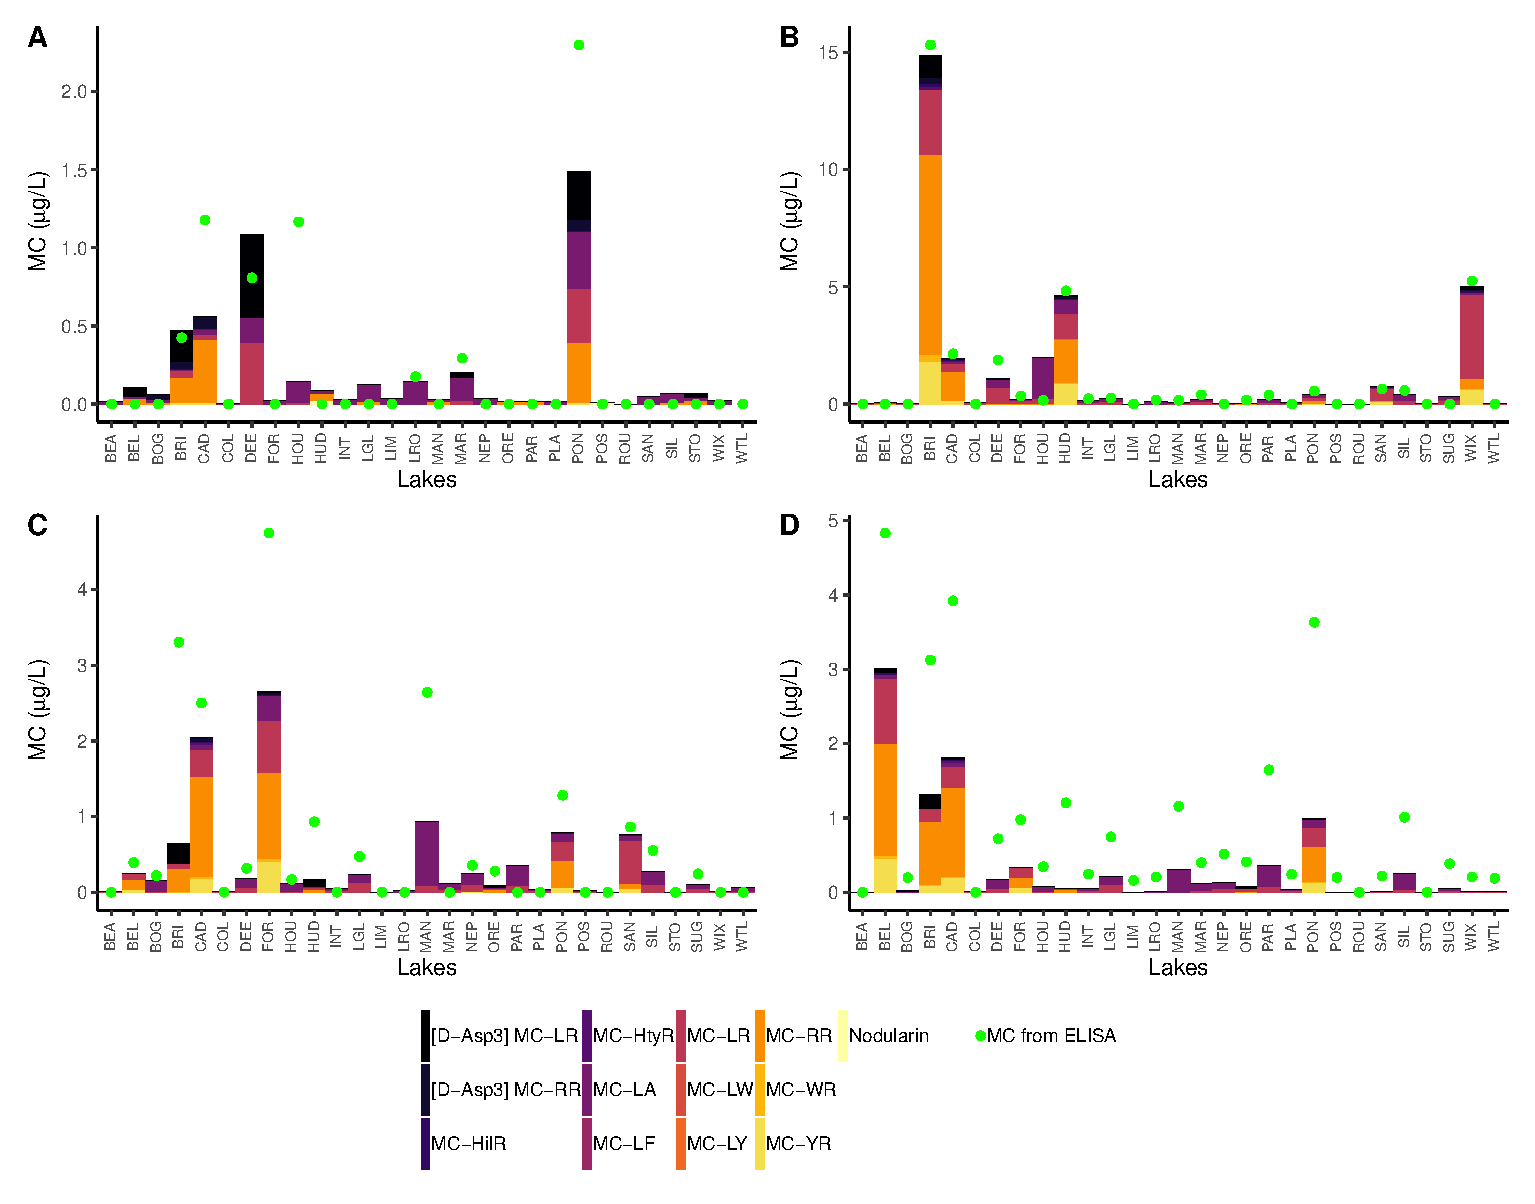
\includegraphics[width=\textwidth]{figures/month}
\caption{
Barplots of MC and their congeners from LC-MS/MS and ELISA  for each lake for the month of 
(A): July, 
(B): August,
(C): September, and
(D): October 
}
	\label{fig:month} 
\end{sidewaysfigure}


%\begin{figure}
%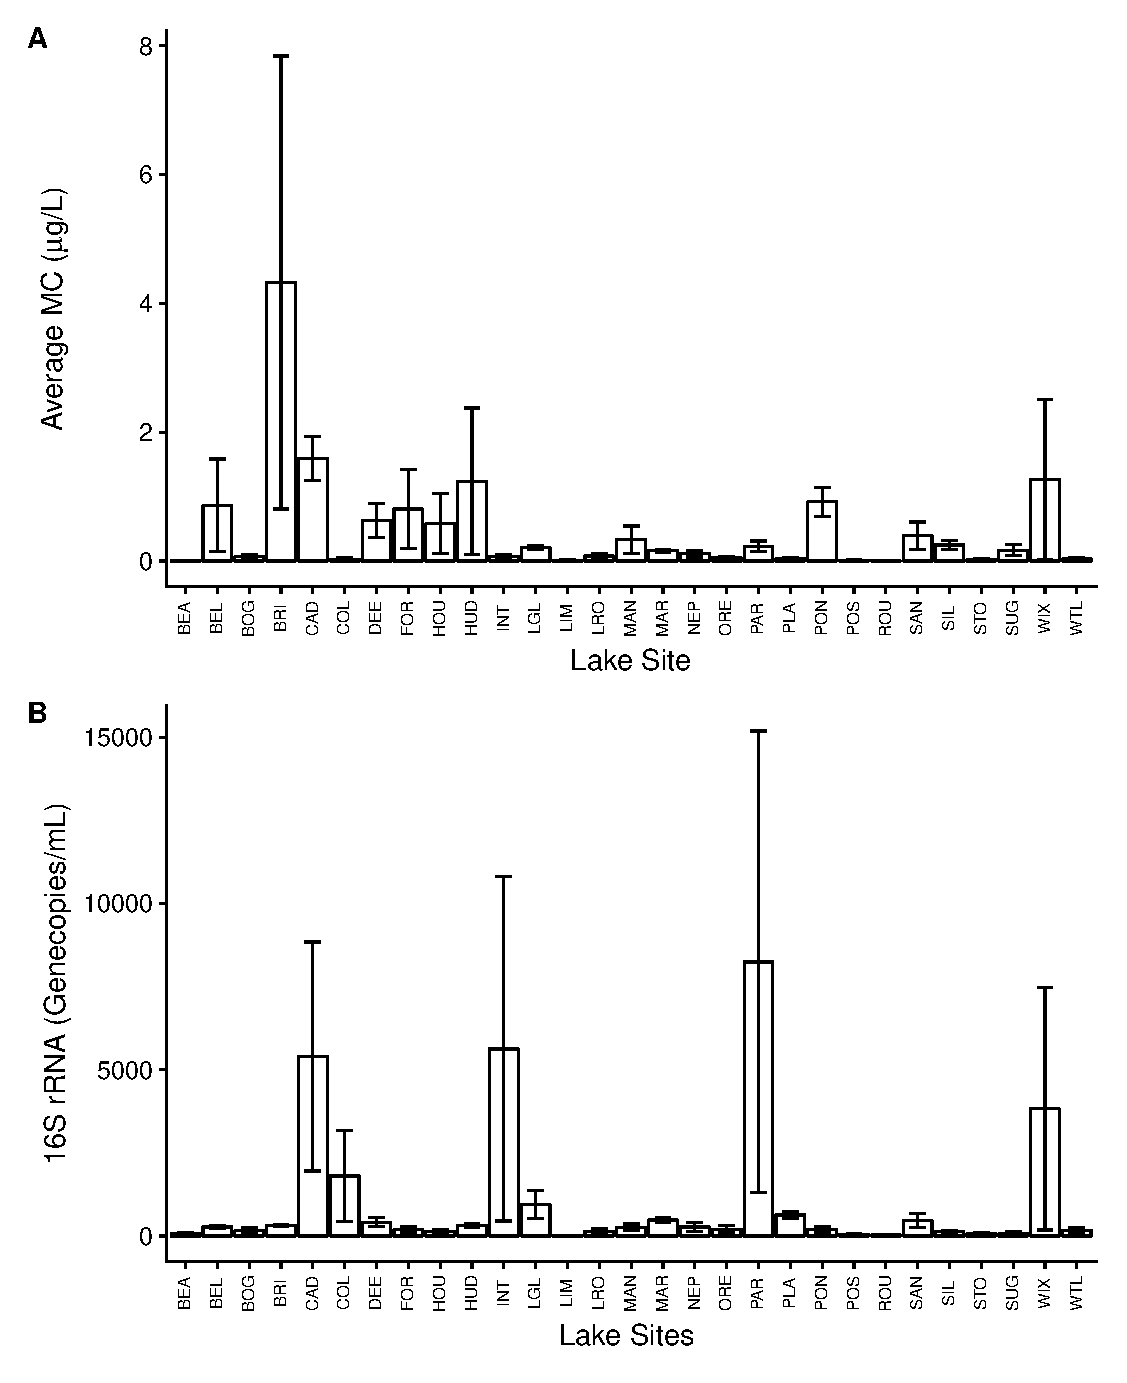
\includegraphics[width=\textwidth]{figures/responsecombine}
%\caption{Average total MC of each lake measured by LC-MS/MS (A). Average \emph{16S rRNA} Genecopies/mL of sample by each lake. (B). Error bars represent one standard deviation of the mean. }
%\label{fig:resbar}
%\end{figure}


% Should I include nutrients?
% Sonde readings (pH, Turbidity, chloro, Conductance)?
\clearpage





\subsection{\emph{A Priori} Hypothesis Test}

In my hypothesis, I expected developed land-use percentage to have a positive influence on MC concentrations. Much of the southern lakes were vastly dominated by developed land such as Belleville, Ore, Brighton, Ford and Bogie Lake. 
Developed land-use percentage plotted had a slight positive effect with $log10$(MC) concentration , however the relationship was not significant  ($\beta=0.59$, $F_{{1,27}}=1.75$ , $p=0.20$)(see figure \ref{fig:developed}) . There were no significant relationship with developed land-use percentage in predicting $log10$(\emph{16s rRNA}) gene copies ($\beta=0.48$, $F_{{1,25}}=1.75$ , $p=0.27$). However, developed land-use had a positive significant relationship with log10(nitrate+nitrite) ($\beta=0.75$, $F_{{1,27}}=1.08$, $p=0.018$)

Forest land-use percentage had a significant negative relationship with $log10$(\emph{16s rRNA}) gene copies ($\beta=-1.42$, $F_{{1,25}}=7.08$, $p=0.013$)(see figure \ref{fig:forest}). Albiet, forest land use did not have a significant effect on $log10$(MC) concentrations ($\beta=-0.34$, $F_{{1,26}}=0.32$, $p=0.57$).

With the surveyed lakes, 17 out of 29 had Zebra mussels found in the month of October. The average MC concentrations with  of Zebra mussles present was 0.568 $\mu$g/L, and absent with 0.305 $\mu$g/L. Using a two sample Student's t-test, we fail to reject the null where difference of the mean is greater than 0 ($t=1.14$, $df=107$, $p=0.13$). We also did not find any significant relationship with the mussel counts and mass with predicting MC concentration.

\begin{figure}
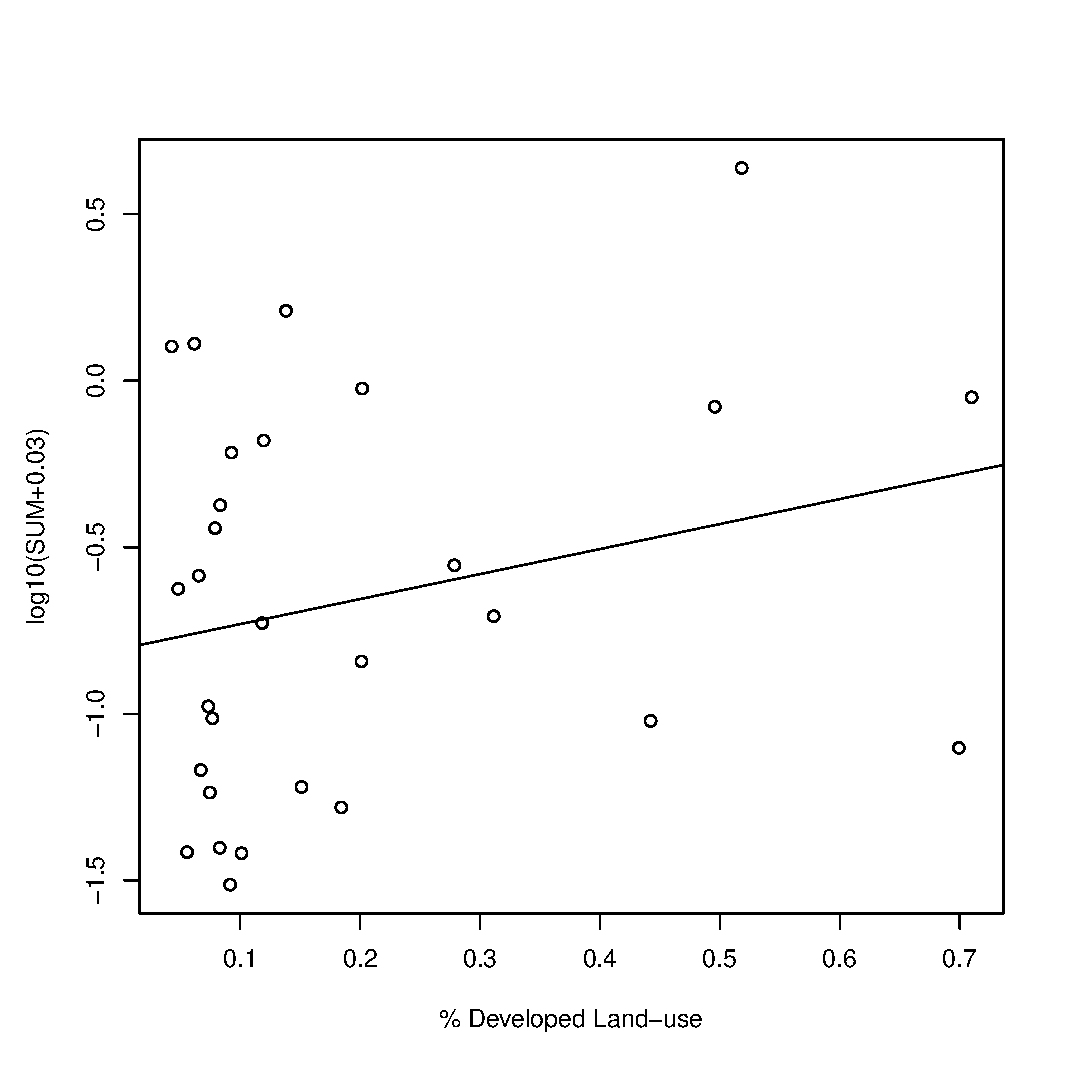
\includegraphics[width=\textwidth]{figures/developed}
\caption{A slight positive relationship between $log10(MC)$ and developed land use. ($\beta=-0.59$, $F_{{1,27}}=1.75$, $p=0.20$)}
\label{fig:developed}
\end{figure}

\begin{figure}
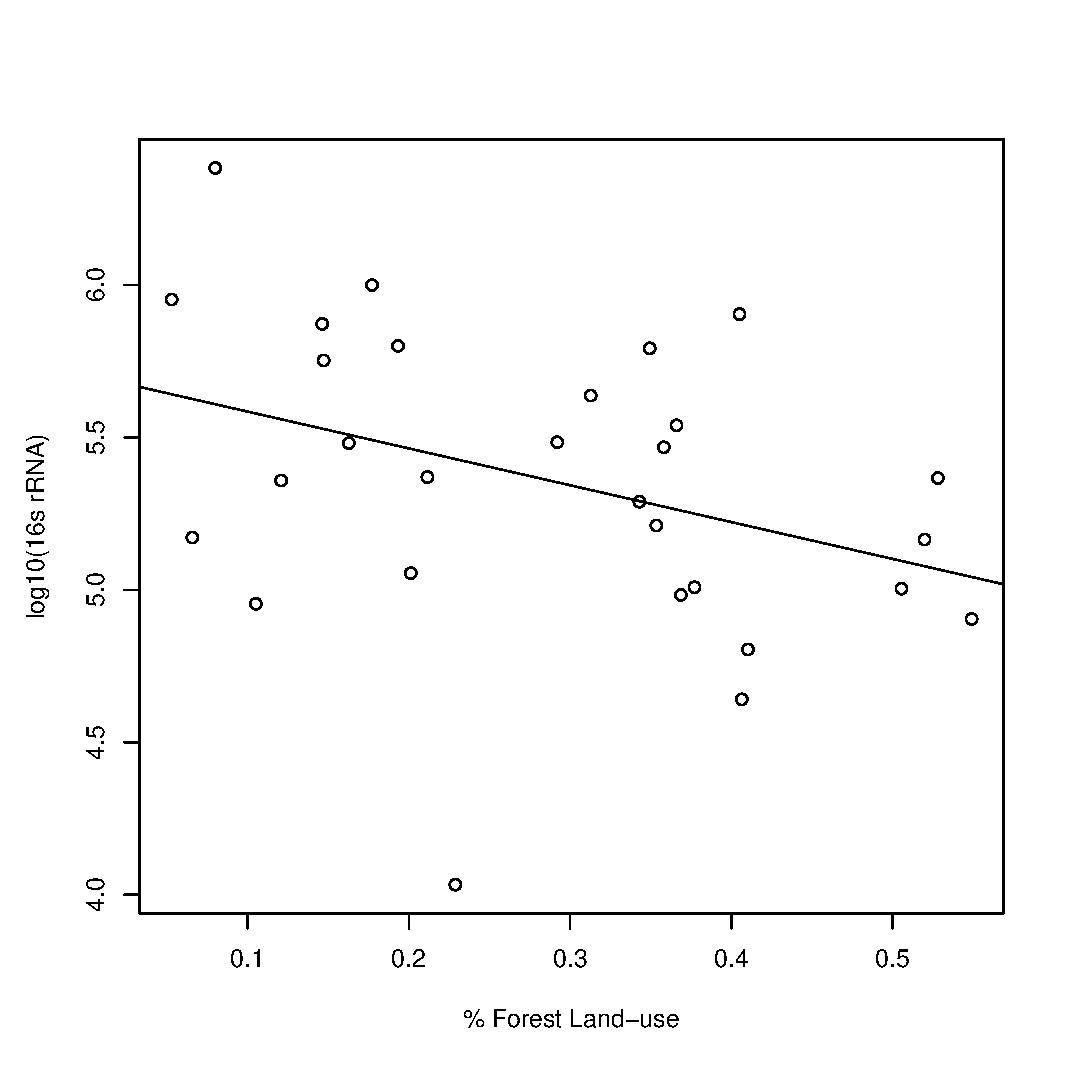
\includegraphics[width=\textwidth]{figures/forest}
\caption{A negative relationship between $log10(MC)$ and forest land use. ($\beta=-1.42$, $F_{{1,25}}=7.08$, $p=0.013$)}
\label{fig:forest}
\end{figure}

\clearpage

\subsection{Exploratory Analysis}

With our model selection, a correlation matrix analysis was done to observe any possible collinear relationships between our predictor variables. The correlation matrix analysis showing only significant relationships and arranged by the anglular order of eigenvectors and identified few correlated variables  (see \ref{matrix}, and see \ref{fig:matrixfull} for the full correlation values). In our correlation matrix analysis, we observed a few relationships that may be meaningful. We found turbidity positively correlated with orthophosphate, total phosphorus, total Kejldahl nitrogen, water temperature, phycocyaninin and chloraphyll. Chlorophyll is positively correlated with \emph{mcye}, phycocyanin, \emph{16S rRNA}, total Kejldahl nitrogen and orthophosphate. Conductance was found to have negative relationship with precipitation.
Developed land-use is positively correlated with nitrate+nitrite, total nitrogen and conductance.
Watershed area was positive correlated with Zebra mussel mass.
Agriculture had a positive relationship with nitrate+nitrite,
Forest land-use had negative correlation with total Kejldahl nitrogen, total nitrogen, conductivity, ammonia, nitrate+nitrite and total nitrogen to total phosphorus ratio.
Precipitation had negative correlation with total nitrogen, orthophosphate and conductivity.

\begin{sidewaysfigure}[!hp]

  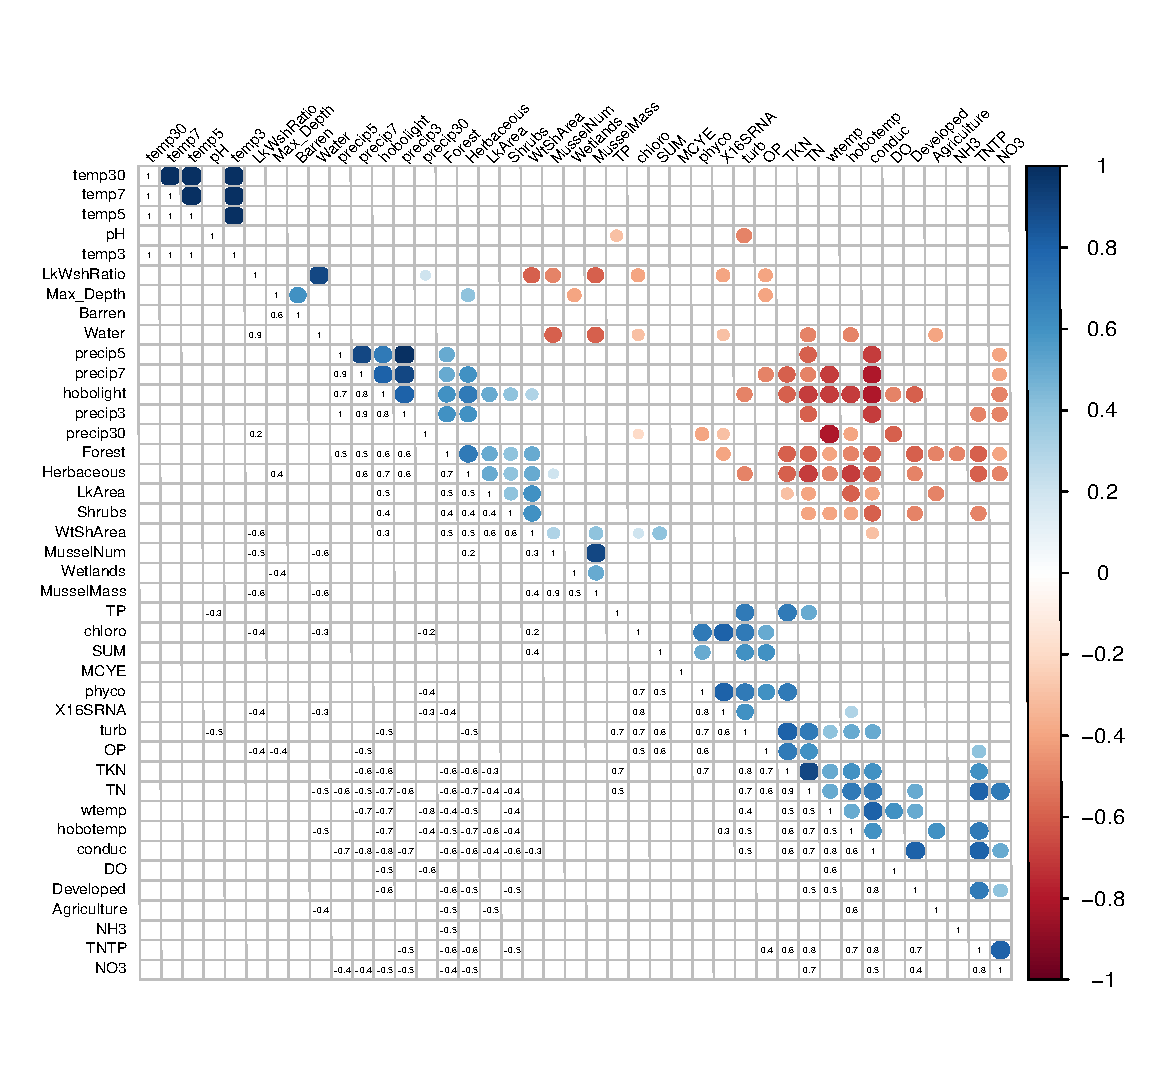
\includegraphics[width=0.7\textwidth]{matrix}
  \vspace*{-10mm}
  \caption{
  Correlation matrix with calculated Pearson coefficient in the lower triangle, and a graphical representation of coefficient value in the upper triangle. Each pair was tested for association between paired variables with Pearson's product moment correlation with relationships not shown if $\alpha>0.05$. Data matrix was arranged by the angular order of the eigenvectors.}
  \label{matrix}
\end{sidewaysfigure}

\clearpage

\subsection{Feature Selection}

From our best subset analysis with the largest subset size of 3 (nvmax=3),  orthophosphate, \emph{mcyE}, turbidity, max depth,  lake area to watershed ratio, barren land-use and precipitation 3 days prior to sampling were frequently chosen  predictor variables for MC concentration (see figure \ref{subset}).


%Proper way to assess collinearity by linear regression? A caused by B and B caused by A?
From our data, $log10$(Orthophosphate) was shown to be positively correlated with $log10$(turbidity) from our exploratory analysis, with a simple linear regression analysis, the relationship is slightly significant ($\beta=0.57$, $F_{{1,26}}=3.13$, $p=0.08$). The regression did have outliers, with the two data points removed the relationship is significant ($\beta=0.17$, $F_{{1,25}}$, $p=0.01$) (see \ref{fig:plot1}). We avoid including either $log10$(orthophosphate) or $log10$(turbidity) in our models together.
%All other variables did not have any significant correlations with eachother.
%From backward stepwise regression, eliminated  contained 3 variables, orthophosphate, max depth and turbidity.
With $log10$(\emph{mcyE}) as a single predictor in a linear mixed model shown to have a significant relationship with $log10$(MC), however we are missing data from July ($N=91$) which does not allow us to use the full dataset ($\beta=0.15$, $F_{{1,72}}$, $p=0.002$).

We found $log10$(turbidity) as the best single predictor. The relationship was significant with predicting $log9$(MC) concentration in a linear mixed-effect model ($\beta=0.55$, $F_{{1,27}}=5.90$, $p=0.02$) (see \ref{fig:plot2}). However, with $log10$(orthophosphate) as a single predictor the relationship is almost significant ($\beta=0.35$, $F_{{1,26}}=3.13$, $p=0.07$) (see \ref{fig:plot2}).  The best model for predicting MC is turbidity as the sole predictor. Adding additional predictors did not significantly improve the model.

For predicting the $log10$(\emph{16s rRNA}) gene copies, chloraphyll, agriculture land-use and average temperature 3 and 30 days prior to sampling and precipitation 5 days before sampling were investigated for building our model (see figure \ref{subset2}). Precipitation and temperature data did not have significant relationship and was eliminated from the model. Agriculture percent land-use found to be the best predictor for \emph{16s rRNA} ($\beta=0.70$, $F_{{1,26}}=5.10$, $p=0.03$)(figure \ref{fig:agriculture})


\begin{figure}[!ht]
  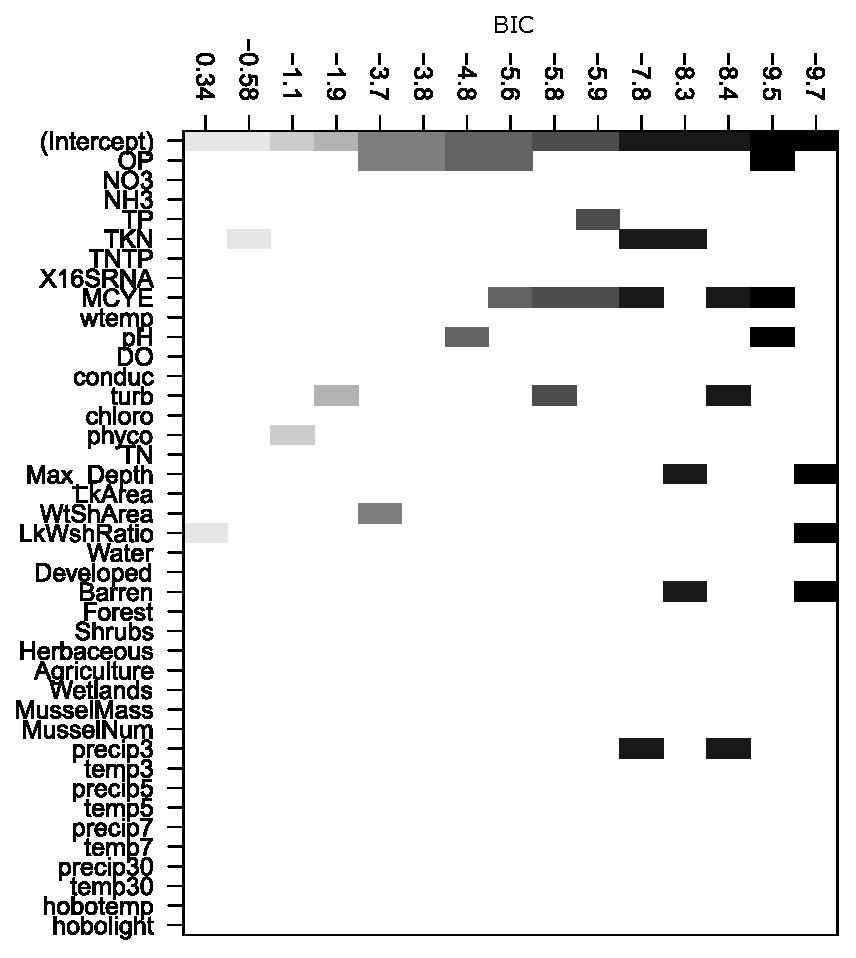
\includegraphics[angle=90,height=8cm, width=\textwidth]{Subset}
  \caption{Subset regression analysis with MC Sum from LC-MS/MS as response variable. Each row is a model. Variable is included in the model it is represented as a black rectangle. The BIC is plotted on the y axis where the lowest value is higher up on the axis.}
  \label{subset}
\end{figure}

\begin{figure}
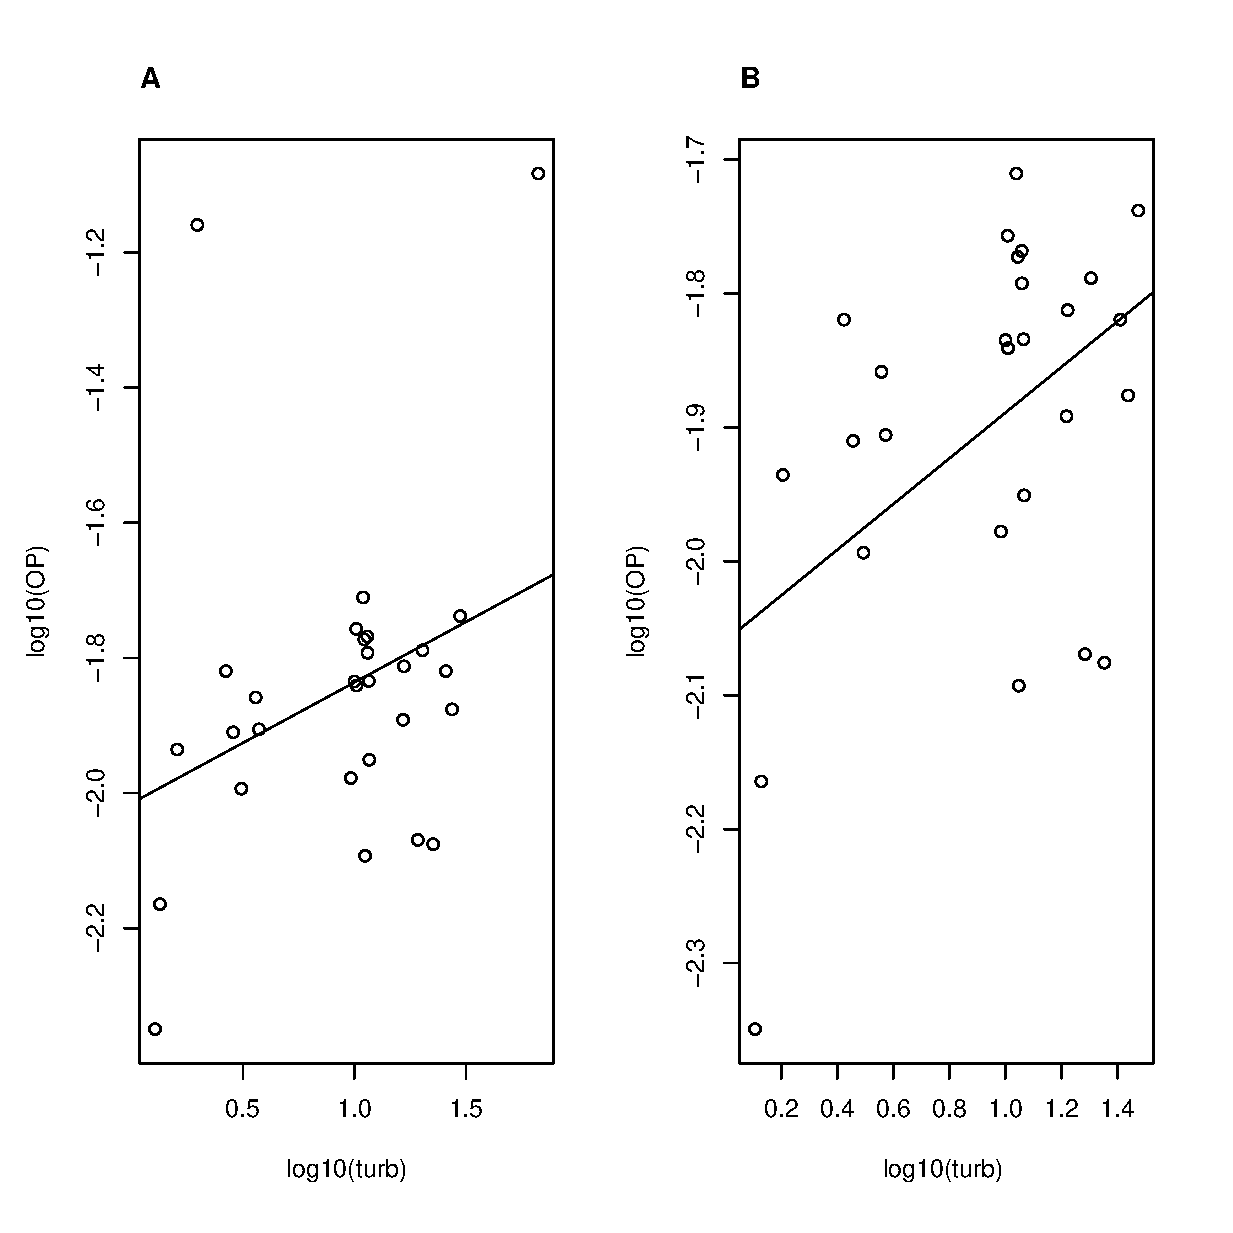
\includegraphics[width=\textwidth, height=11cm]{figures/plot1}
\caption{
(A): Positive relationship with average $log10$(OP) with average $log10(turb)$ ($\beta=0.57$, $F_{{1,26}}=3.13$, $p=0.08$).
(B): With two outliers removed, the relationship between $log10(OP)$ and $log10(turb)$ was signifigant  ($\beta=0.17$, $F_{{1,25}}$, $p=0.01$).
}
\label{fig:plot1}
\end{figure}

\begin{figure}
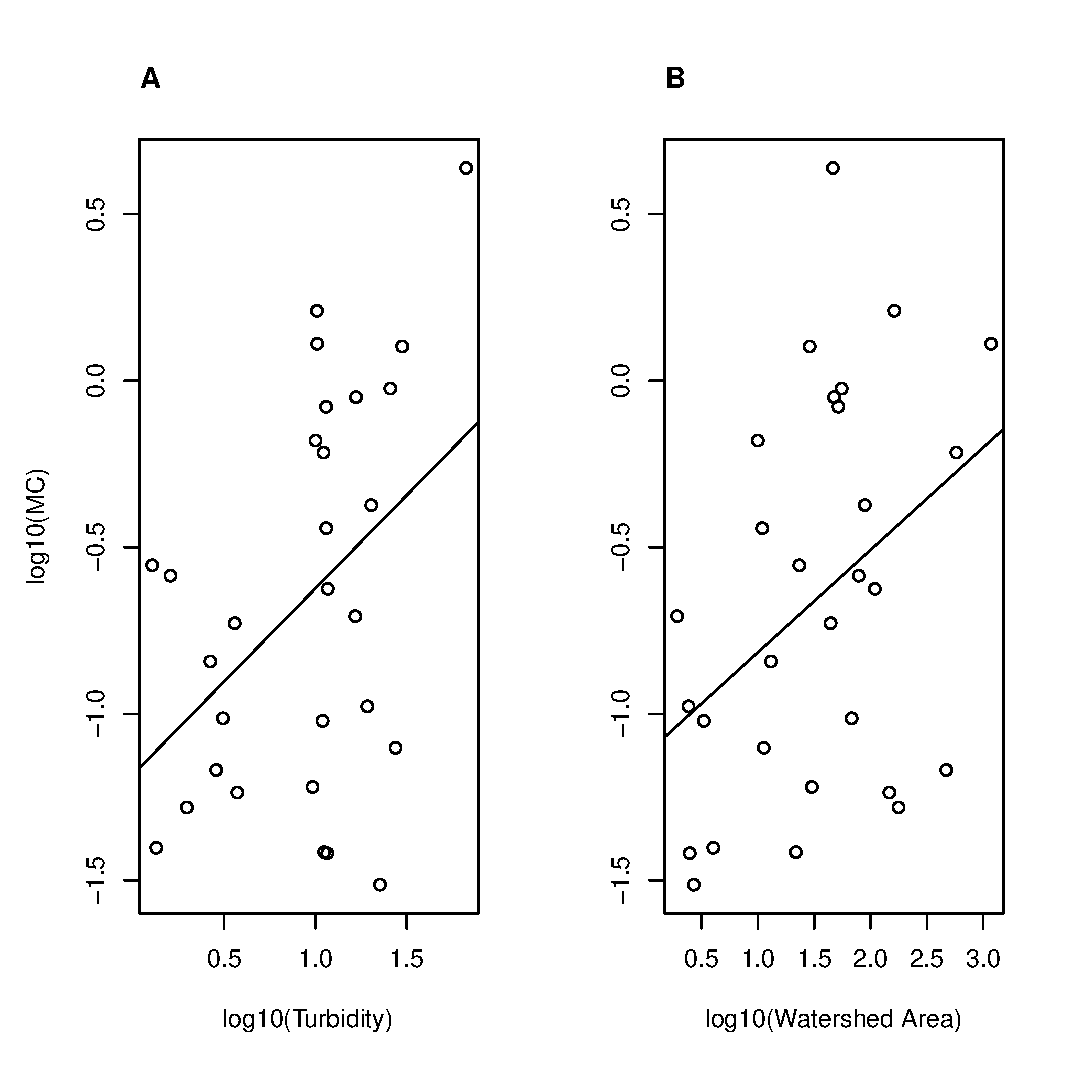
\includegraphics[width=\textwidth, height=11cm]{figures/plot2}
\caption{
(A): Positive relationship between average $log10$(MC) with average $log10(turb)$ ($\beta=0.55$, $F_{{1,27}}=5.90$, $p=0.02$)
(B): Positive relationship between average $log10(MC)$ and average  $log10$(OP) ($\beta=0.35$, $F_{{1,26}}=3.13$, $p=0.07$). 
Turbidity is our best predictor variable for MC. Orthophosphate is nearly significant predictor}
\label{fig:plot2}
\end{figure}

\begin{figure}[!ht]
  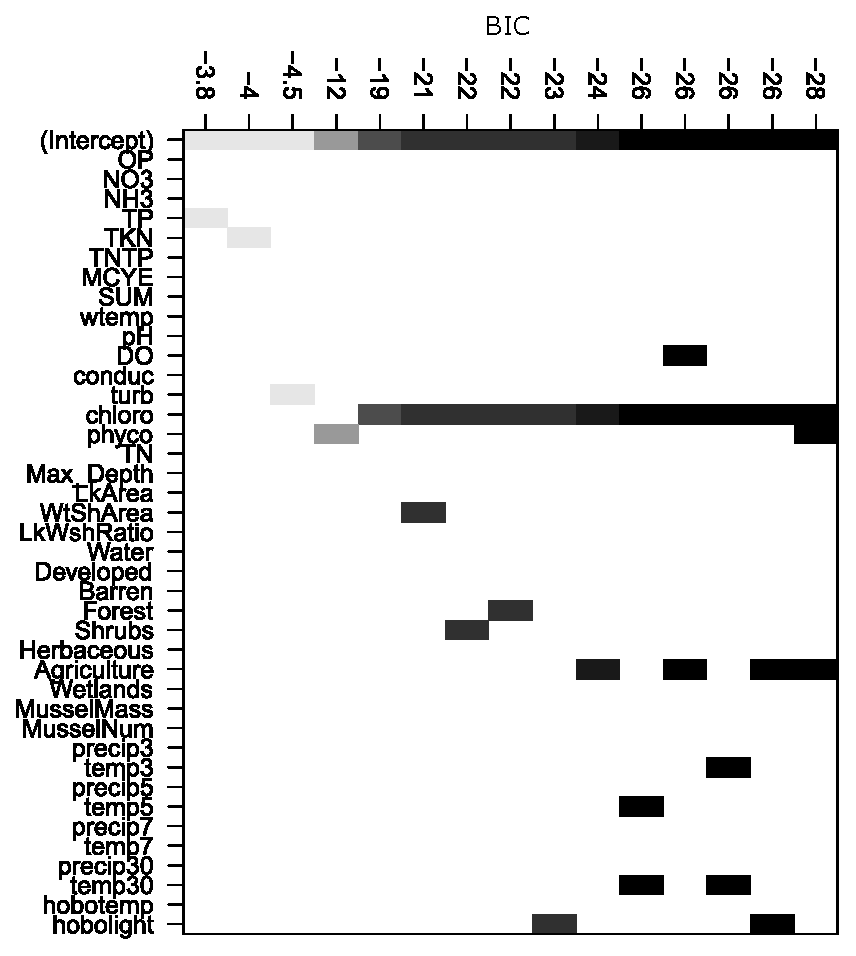
\includegraphics[angle=90,height=8cm, width=\textwidth]{Subset1}
  \caption{Best Subset: \emph{16s rRNA} Gene copies as response variable}
  \label{subset2}
\end{figure}

\begin{figure}[!ht]
  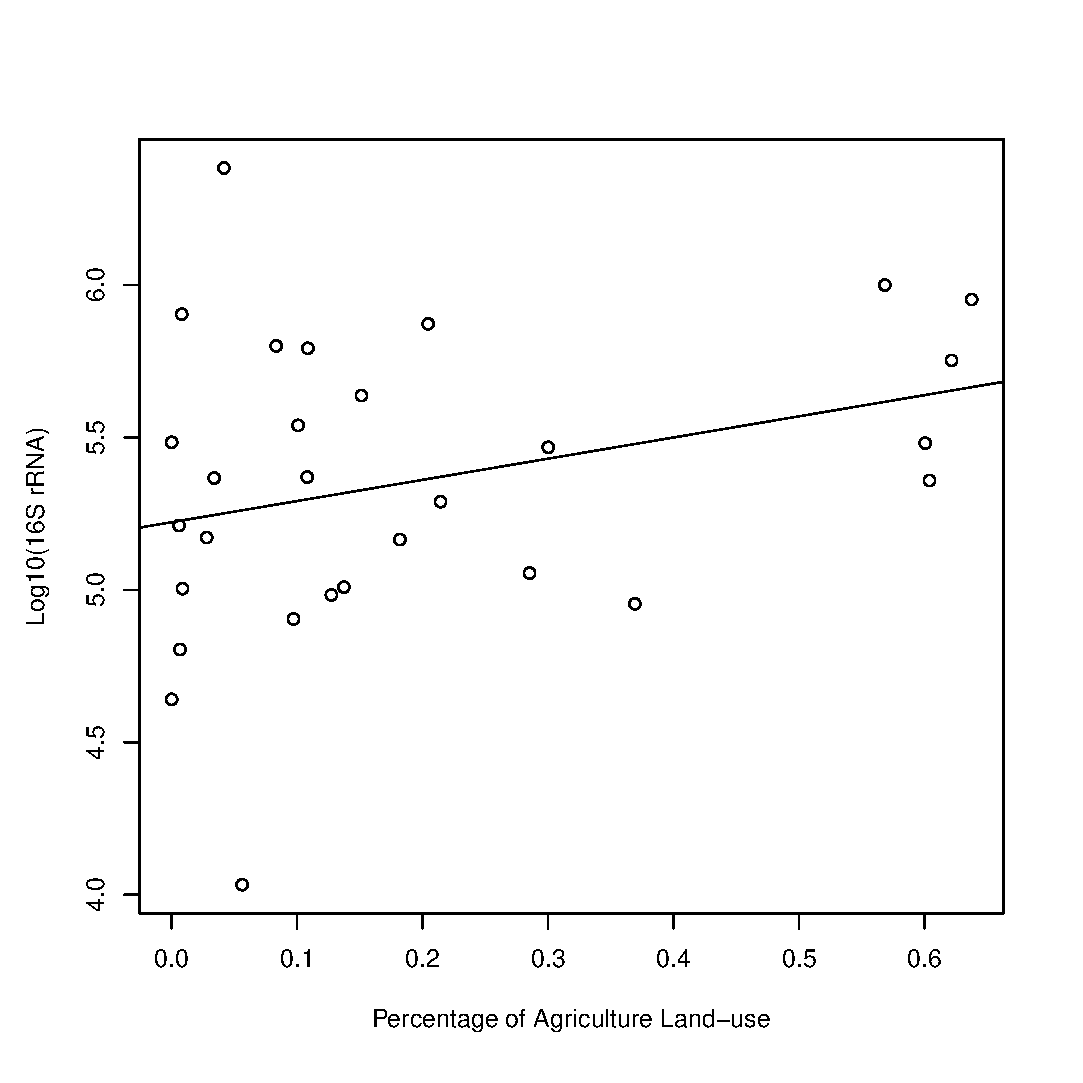
\includegraphics[width=\textwidth]{figures/Agriculture}
  \caption{Positive relationship between percent agriculture land-use and $log10$(\emph{16s rRNA}) ($\beta=0.70$, $F_{{1,26}}=5.10$, $p=0.03$)}
  \label{fig:agriculture}
\end{figure}
\clearpage

\section{SPATT}

Out of all 12 congeners, MC-LA, MC-LR, and MC-RR were the most frequently detected congener (see \ref{tab:spattcongener}). Microcystin concentrations from SPATT was mostly detected in lake Paradise, Intermediate Lake, Lake Cadillac and Wixom Lake. Comparing the average results from SPATT to the grab sample, we identified a major difference (see \ref{fig:spattbox}). When average concentration of MC from SPATT and grab sample is ordered by latitude, we found the relative mangitude of microcystin is higher found in the upper latitude of Michigan compared to regular grab sample. In our grab sample, Brighton, Pontiac, Wixom Lake and Lake Cadillac had high average MC with notable \gls{hab}.

\begin{figure}[!hp]
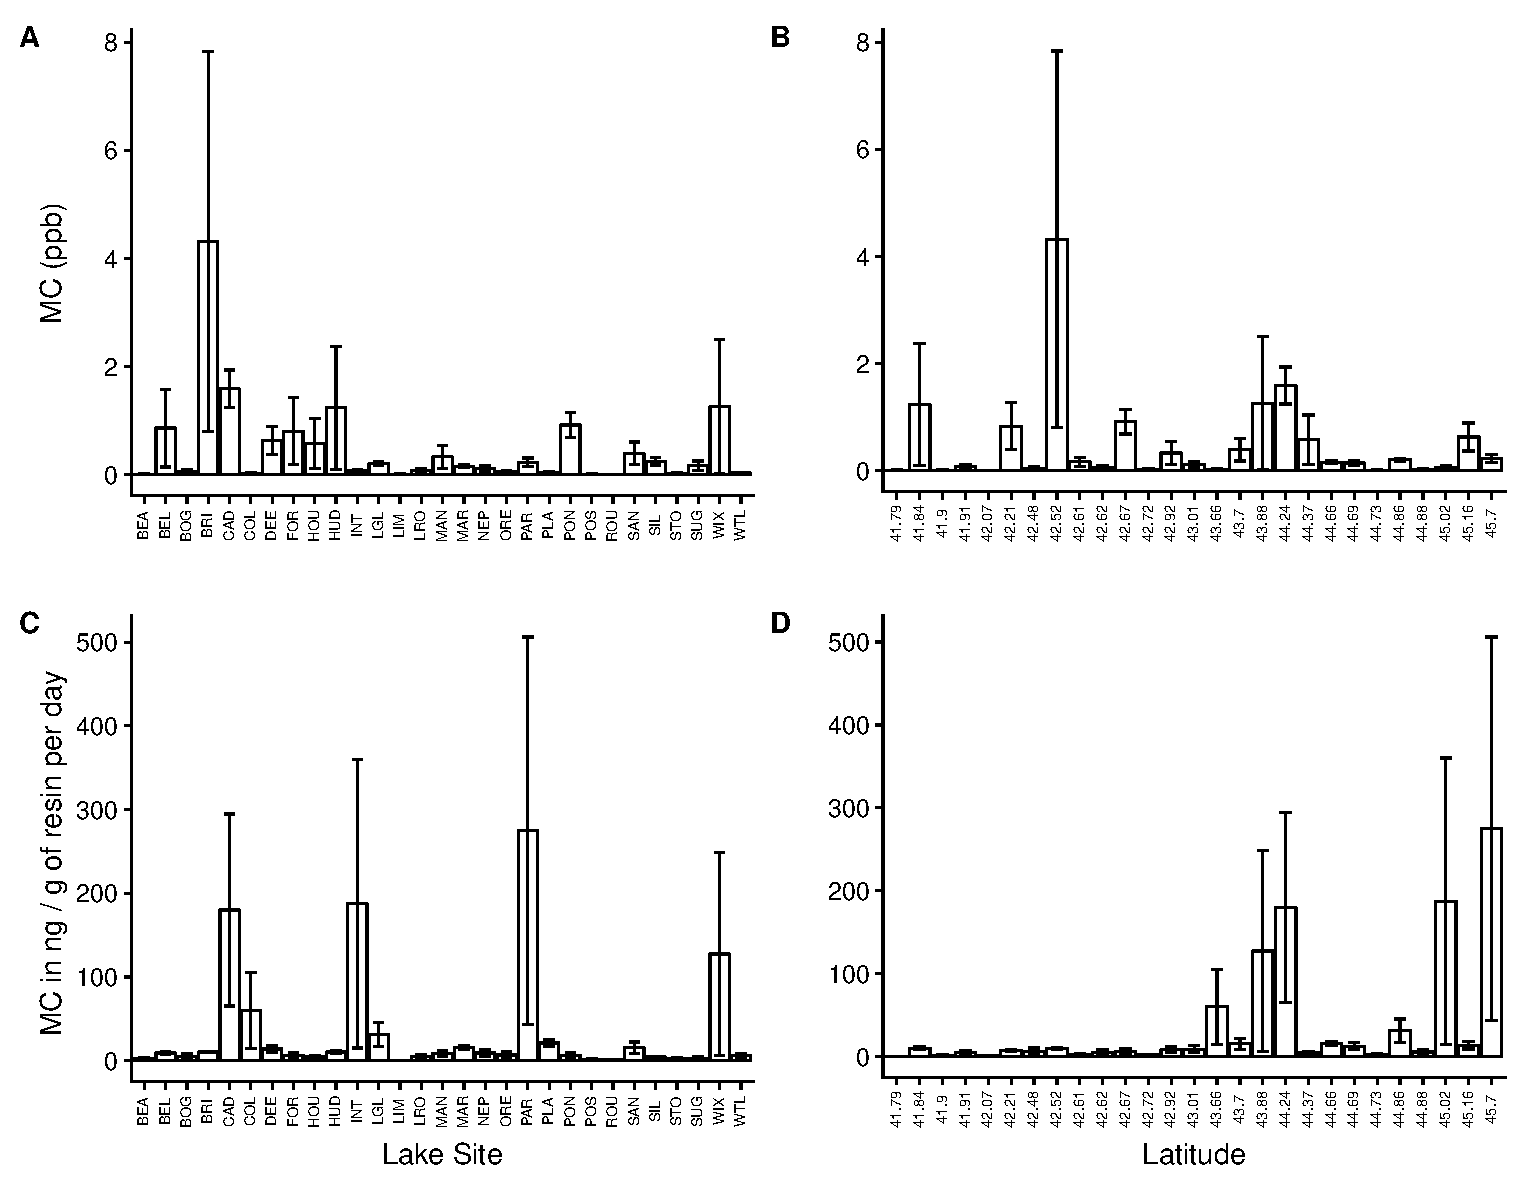
\includegraphics[width=\textwidth]{figures/spatttboxplotlake}
\caption{
Microcystin measured from SPATTS compared to grab sample: and Grab Samples. Average concentration of MC are plotted as bar graphs. Microcystin concentrations analyzed from grab sample are shown in figure (A) arranged by each lake and (B) arranged by latitude. Microcystin concentrations analyzed from SPATT samples are shown in figure (C) arranged by each lake and figure (D) arranged by latitude
}
\label{fig:spattbox}
\end{figure}

\begin{figure}[!ht]
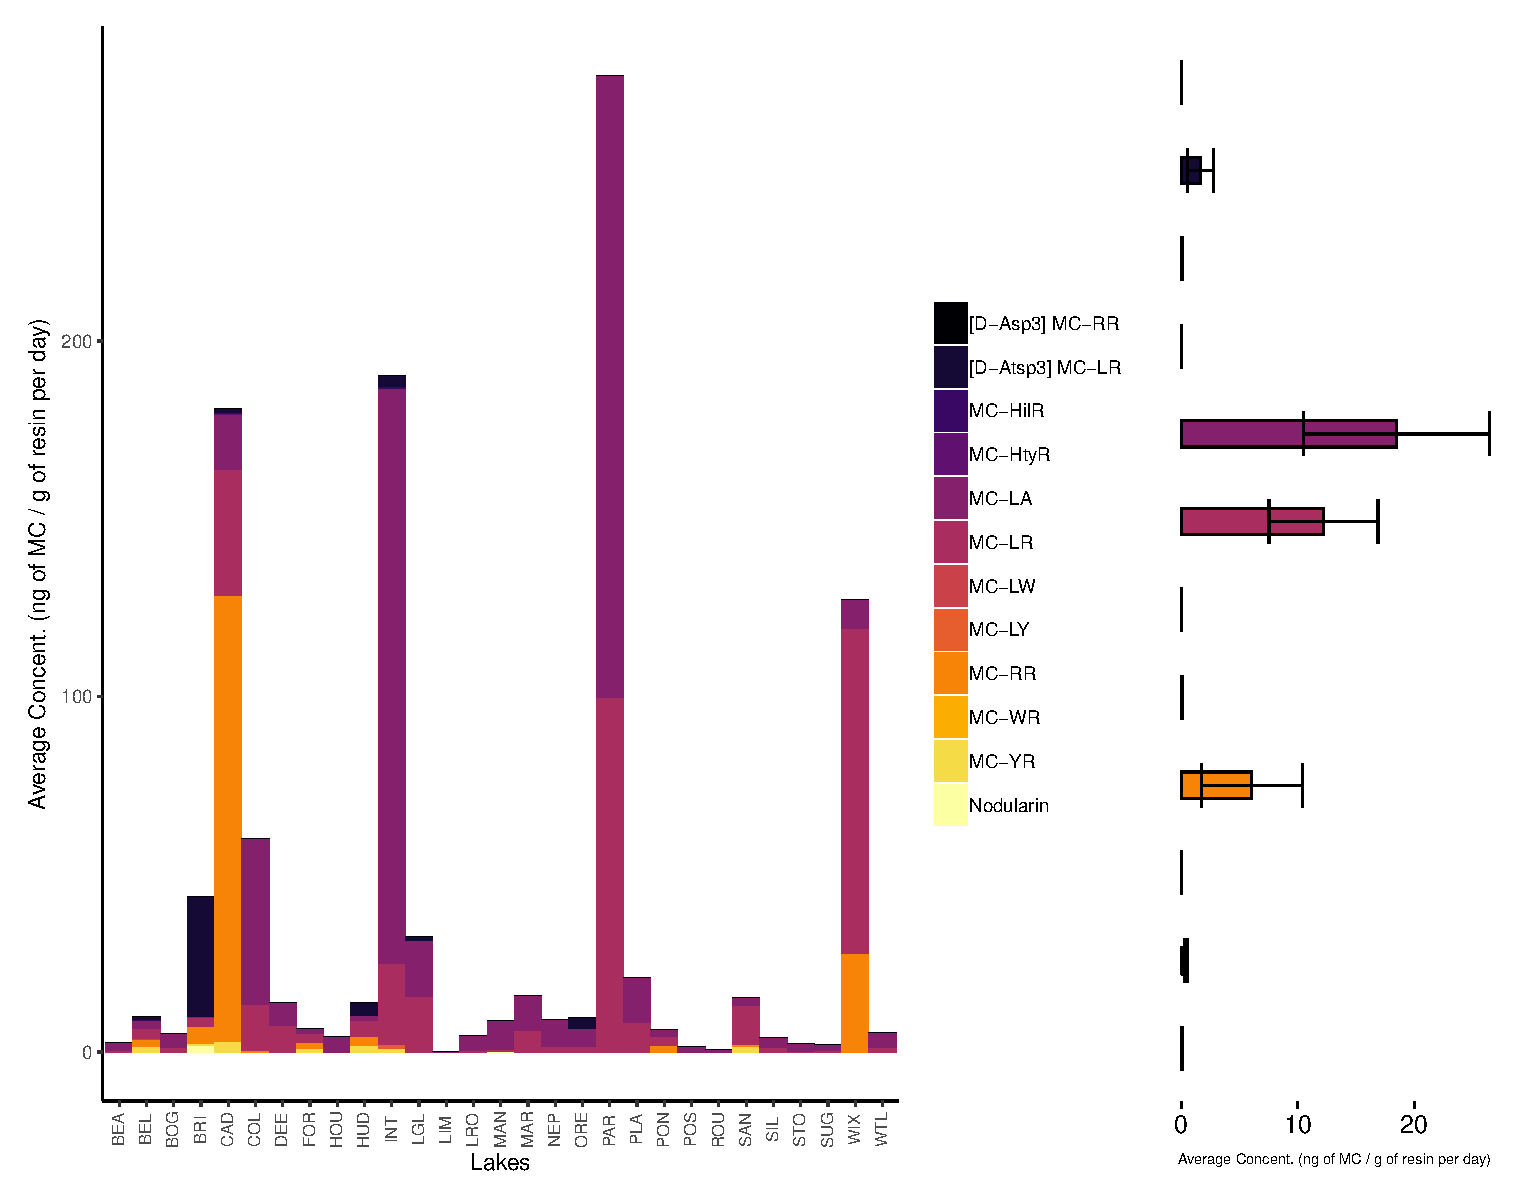
\includegraphics[width=\textwidth]{figures/barspatts}
\caption{Average MC congeners at each lake. Error bars represent one standard deviation of the mean}
\label{fig:barspatts}
\end{figure}

\begin{table}[!ht]
\centering
  \caption{Microcystin Congener from SPATT}
  \label{tab:spattcongener}
\begin{tabular}{@{\extracolsep{5pt}}lccccc}
\\[-1.8ex]\hline
\hline \\[-1.8ex]
Statistic & \multicolumn{1}{c}{N} & \multicolumn{1}{c}{Mean} & \multicolumn{1}{c}{St. Dev.} & \multicolumn{1}{c}{Min} & \multicolumn{1}{c}{Max} \\
\hline \\[-1.8ex]
{[D-Asp3]}MC-RR & 91 & ND & ND & ND & ND \\
MC-RR & 91 & 164 & 1,116 & ND & 10,380 \\
Nodularin & 91 & 2 & 17 & ND & 160 \\
MC-YR & 91 & 10 & 30 & ND & 145 \\
MC-HtyR & 91 & 0 & 2 & ND & 18 \\
MC-LR & 91 & 353 & 1,211 & ND & 8,146 \\
{[D-Asp3]}MC-LR & 91 & 2 & 10 & ND & 92 \\
MC-HilR & 91 & 1 & 6 & ND & 53 \\
MC-WR & 91 & 0 & 1 & ND & 7 \\
MC-LA & 91 & 534 & 2,063 & ND & 13,977 \\
MC-LY & 91 & 1 & 11 & ND & 101 \\
MC-LW & 91 & 0 & 0 & ND & 0 \\
MC-LF & 91 & 0 & 2 & ND & 18 \\
Total MC & 91 & 1,066 & 3,273 & ND & 22,124 \\
\hline \\[-1.8ex]
\multicolumn{6}{r}{Values are expressed as (ng of MC / gram of resin)} \\
\multicolumn{6}{r}{ND=No Detects} \\
\end{tabular}
\end{table}


\clearpage
\newpage


\subsection{Discussions}

Comparing the results between MC concentrations and \emph{16s rRNA}, we can see a difference in figure \ref{fig:resbar}.
Lake turnover, winter stable, spring mix, summer stable, fall mix. 
Microcystin concentration tells a different story compared to \emph{16s rRNA}. This curve is to be expected due to warmer temperature as our data does follow this pattern (see figure \ref{fig:hobo}).

In our first hypothesis, I wanted test if disturbance from developed land is associated with \gls{hab} and if it has an affect on nutrient concentration.  From our data, we did not find a significant relationship between developed land use and MC concentrations or \emph{16s rRNA}. However, we did find developed land use having some effect with nitrate+nitrite.

Forest has negative correlation with NUTRIENTS

Disturbances of flora contributes to lower nutrient retention and hydrological impacts that can cause more blooms \cite{anderson_harmful_2002, codd_cyanobacterial_2000, fraterrigo_influence_2008}.
\gls{mc} could increase as developed is more prevalent in the lake's watershed.


Bioavailability of phosphorus is pH dependent, where most is available between when in alkaline conditions greater \cite{lucas_relationships_1961}.
Mostly all of our sampled lakes were mostly alkaline conditions averaging around 8.53$\pm$0.37 pH ranging from 7.44 to 9.94.

Wixom lake is very unique, it has the largest watershed amongst all our surveyed lake and has visually one of the largest extent


%Dissolved oxygen averaged around 12.98$\pm$20.8 mg/L of \ch{O2}.

% FORMS OF NUTRIENTS TODO revise this, expand it
In controlled lab experiments, nutrients such as inorganic nitrogen or phosphorus are found to be limiting growth factors. In a  when \emph{Microcystis aereginosa} grown in the laboratory \cite{xiao_colony_2018, yema_role_2016}.

% revise this and put more work into this TODO
Cyanobacteria are versatile as they can acquire nutrients under extreme conditions. They can utilize a process called quorom sensing which they coordinate with each other by using a signaling hormone acylated homoserine lactones \cite{van_mooy_quorum_2012}. They also can create a network of cells which work together as a unit, often as seen as a layer of green goo floating on top of water.  There are very robust organisms, as some can change their buoyancy by modulating the intracellular gas vesicles gives them a competitive advantage over other species for seeking light \cite{feng_how_2018}.\emph{Microcystis} can form a complex colony made by a mucilage structure which can be bouyant due to high concentration of dissolved oxygen \cite{xiao_colony_2018}. % TODO expand how co2 gets pumped into gas vesicles
Most of the cyanotoxin are intracellular, however with increase turbulence from wind and precipitation can release more toxins due to cell lysis either from cell apoptosis or from mechanical abruption which release \cite{rohrlack_fate_2007}. % TODO cyanophages, viruses 



%A study in South Korea found 3-week lagged water temperature,dissolved oxygen and pH with to correlate with each other in their models \cite{ahn_evaluation_2011}.

%Growing cyanobacteria measurements taken at the same time . Their is an assumption being made.

%Total nitrogen was found to explain the variance of MC concentrations \cite{taranu_predicting_2017}.

%Man-made lakes are found to be twice as higher concentrations in cylindrospermonsin \cite{loftin_cyanotoxins_2016}.


%Low-nutrient lakes can still exhibit blooms.
 %This can complicate our model as this is not accounted for.

%QPCR results as a response variable comes with complication as this does not distinguish alive or dead cyanobacteria.




%Water sampling for nutrient is difficult. Time series data, nutrient dynamic. Continuous measurements  water data would be best, but for a large survey its almost impractical. Other organisms compete with these common nutrients. Aquatic macrophytes largely acquire dissolved phosphorus. Time between sampling the lake at the peak of the bloom and the flush of nutrient inputs can be lagged, and most likely different depending on each lakes morphology. Biological properties are not necessarily linear. One thing to consider here is the sampling frequency. We sampled once a month for four months, which gives four sampling results for each lake. This may not explain everything about each lake.

% How pH and DO has an influence on nutrient availability


The results from SPATT seemed to suggest the lakes we found to have low microcystin from our grab sample missed other \gls{hab}. When lakes were ordered by latitude, it also suggest lakes found in the upper latitude of Michigan may had higher frequency of \gls{hab}.

We suggest there is another factor that explains the higher magnitude of microcystin. We started to observe biofilm to accumulate on the SPATT bags. The biofilm was more notable in lakes that had significant blooms such as Brighton, Pontiac, and Wixom Lake. Initially we did not expect this would effect the capacity of the SPATT, but this data may suggest this. In our next year of survey we will test the hypothesis if the biofilm has a negative effect of microcystin adsorption. We may need to dispatch the SPATT bags more often to prevent biofilm to encase and clog the Nitex mesh bag.




% !TEX root = main.tex
\chapter{CONCLUSION}

From our analyses, we found ELISA and \gls{lcmsms} to have good agreement except in the month of October where ELISA generally reported high values. We believe this could be due to the cross reactivity with non MCs, particularly degradation products common in the fall. We also observed some discrepancies with the SPATT compared to our grab samples. This could have been due to where some lakes had substantial biofilm encasing the SPATT bags, in particular to lakes with \gls{hab}, preventing the adsorbtion of MC. In our next year of survey we will test the hypothesis if the biofilm has a negative effect of MC adsorption.

It is difficult to realistically model \gls{hab} as it involves with dynamic relationships between abiotic and biotic factors, cyanobacteria growth and cyanotoxin production. We identified orthophosphate to be associated with \gls{mc}, but not neccessarily with cyanobacteria(in terms of gene copies). We also found turbidity which can be a surrogate parameter of other factors to be also a good corrlate. However, turbidity can be caused from cyanobacterial cells. In general there are no best models in an ideal sense, but statistical modeling can help identify meaningful relationships. Point sampling does not encapsulate all the complex relationship and does not explain subtle changes. Confounding variables such as unaccounted disturbances not measured from our survey is not accounted. Even with the use of SPATT, there are still some challenges to overcome. Predicting \gls{mc} alone may not be the most ideal approach, but still worthwhile to investigate nonetheless. Other previous studies built predictive models based using cyanobacterial cell counts, biomass and species composition as a response variable as its most likely associated with \gls{hab} \cite{moore_richard_cyanobacterial_1993, ahn_evaluation_2011, jiang_statistical_2008, beaulieu_nutrients_2013, taranu_predicting_2017}. As of writing this thesis, we are still working on identifying and the cyanobacteria. 

In our future work, the use of \gls{qpcr} to measure mRNA or tRNA for gene expression may provide more indepth of what environmental parameters could influence the production of cyanotoxins. The use of \gls{qpcr} has shown to be effective in predicting \gls{hab} \cite{wilson_genetic_2005}. However there is some valid criticism against the use of \gls{qpcr}. First, the quantified concentrations of genes are not distinguishable between live or dead cells. There are also limitations of relating gene copies to cell counts or concentrations of cyanotoxins \cite{pacheco_is_2016}. Nevertheless, the use of \gls{qpcr} can be still helpful but should be used in parallel to \gls{lcmsms} and cell counts.

Its important to understand why \gls{hab} is occurring and is worth to investigate further. Using a predictive model is a vital utility for protecting the public from \gls{hab}. Addressing public health is a balance of scientific knowledge, risk assessment of the situation and maximizing available tools at our disposal. 








% The \StartGrizzAppendices command switches the formatting for the
% remainder of the document -- Leave this alone
\StartGrizzAppendices

% Include each separate appendix source file here

\addtocontents{toc}{\vspace{\baselineskip}APPENDICES}
\setcounter{table}{0}
\renewcommand{\thetable}{\Alph{chapter}\arabic{table}}
\GrizzAppendix{Tables and Figures} \label{ch:extra}

\begin{table}[]
	\caption{QPCR Standard Curve Quality Parameters}
	\label{tab:qpcr}
\begin{tabular}{llllll}
Date     & Target   & Slope  & Intercept & $R^2$ & \% Efficiency \\
20170812 & 16s rRNA & -3.182 & 36.225    & 0.925 & 106.199        \\
20170713 & 16s rRNA & -3.382 & 38.225    & 0.916 & 92.877         \\
20170918 & 16s rRNA & -3.835 & 39.687    & 0.999 & 82.284         \\
20171011 & 16s rRNA & -3.961 & 39.121    & 0.963 & 78.841         \\
20170714 & cyraA    & -4.34  & 41.35     & 0.931 & 69.788         \\
20170812 & cyraA    & -4.126 & 41.001    & 0.93  & 74.734         \\
20170918 & cyraA    & -3.116 & 37.538    & 0.978 & 109.35         \\
20171011 & cyraA    & -3.219 & 36.793    & 0.951 & 104.5          \\
20170714 & mcyE     & -3.279 & 36.131    & 0.999 & 101.832        \\
20170812 & mcyE     & -3.486 & 38.108    & 0.977 & 93.573         \\
20170918 & mcyE     & -3.541 & 37.72     & 0.944 & 91.608         \\
20171011 & mcyE     & -3.398 & 36.844    & 0.974 & 96.94          \\
20170714 & sxtA     & -4.591 & 42.602    & 0.92  & 65.13          \\
20170812 & sxtA     & -3.262 & 37.913    & 0.965 & 102.568        \\
20170918 & sxtA     & -3.236 & 37.905    & 0.966 & 103.715        \\
20171011 & sxtA     & -3.205 & 37.757    & 0.958 & 105.118       
\end{tabular}
\end{table}

\newpage

\begin{table}[]
	\caption{AQ1 Standard Curve Quality Parameters}
	\label{tab:aq1}
\begin{tabular}{llllll}
Date     & $R^2$  & Slope & Intercept & Carryover & Analysis        \\
20170707 & 0.9993 & 2.61  & 0.00      & 0.20      & Orthophosphate  \\
20170711 & 0.9996 & 1.63  & -0.29     & -0.90     & Ammonia         \\
20170711 & 1      & 15.99 & -0.51     & 0.30      & Nitrate+nitrite \\
20170711 & 1      & 16.49 & -0.51     & 0.10      & Nitrate+nitrite \\
20170807 & 0.9993 & 2.43  & 0.00      & 0.20      & Orthophosphate  \\
20170808 & 0.9993 & 47.36 & -0.90     & 0.80      & Nitrate+nitrite \\
20170808 & 1      & 16.57 & -0.47     & 0.40      & Nitrate+nitrite \\
20170809 & 0.9998 & 1.70  & -0.20     & -1.80     & Ammonia         \\
20170814 & 0.9998 & 2.35  & 0.00      & 0.60      & Nitrate+nitrite \\
20170814 & 0.999  & 18.50 & -0.43     & 0.20      & Nitrate+nitrite \\
20170817 & 0.9995 & 1.59  & -0.33     & 0.30      & Ammonia         \\
20170909 & 0.9996 & 2.94  & -0.01     & -0.20     & Orthophosphate  \\
20170912 & 0.9996 & 1.67  & -0.09     & 0.70      & Ammonia         \\
20170913 & 0.9997 & 17.72 & -0.53     & -0.90     & Nitrate+nitrite \\
20170913 & 0.9996 & 1.67  & -0.09     & 0.70      & Ammonia        
\end{tabular}
\end{table}


\begin{figure}
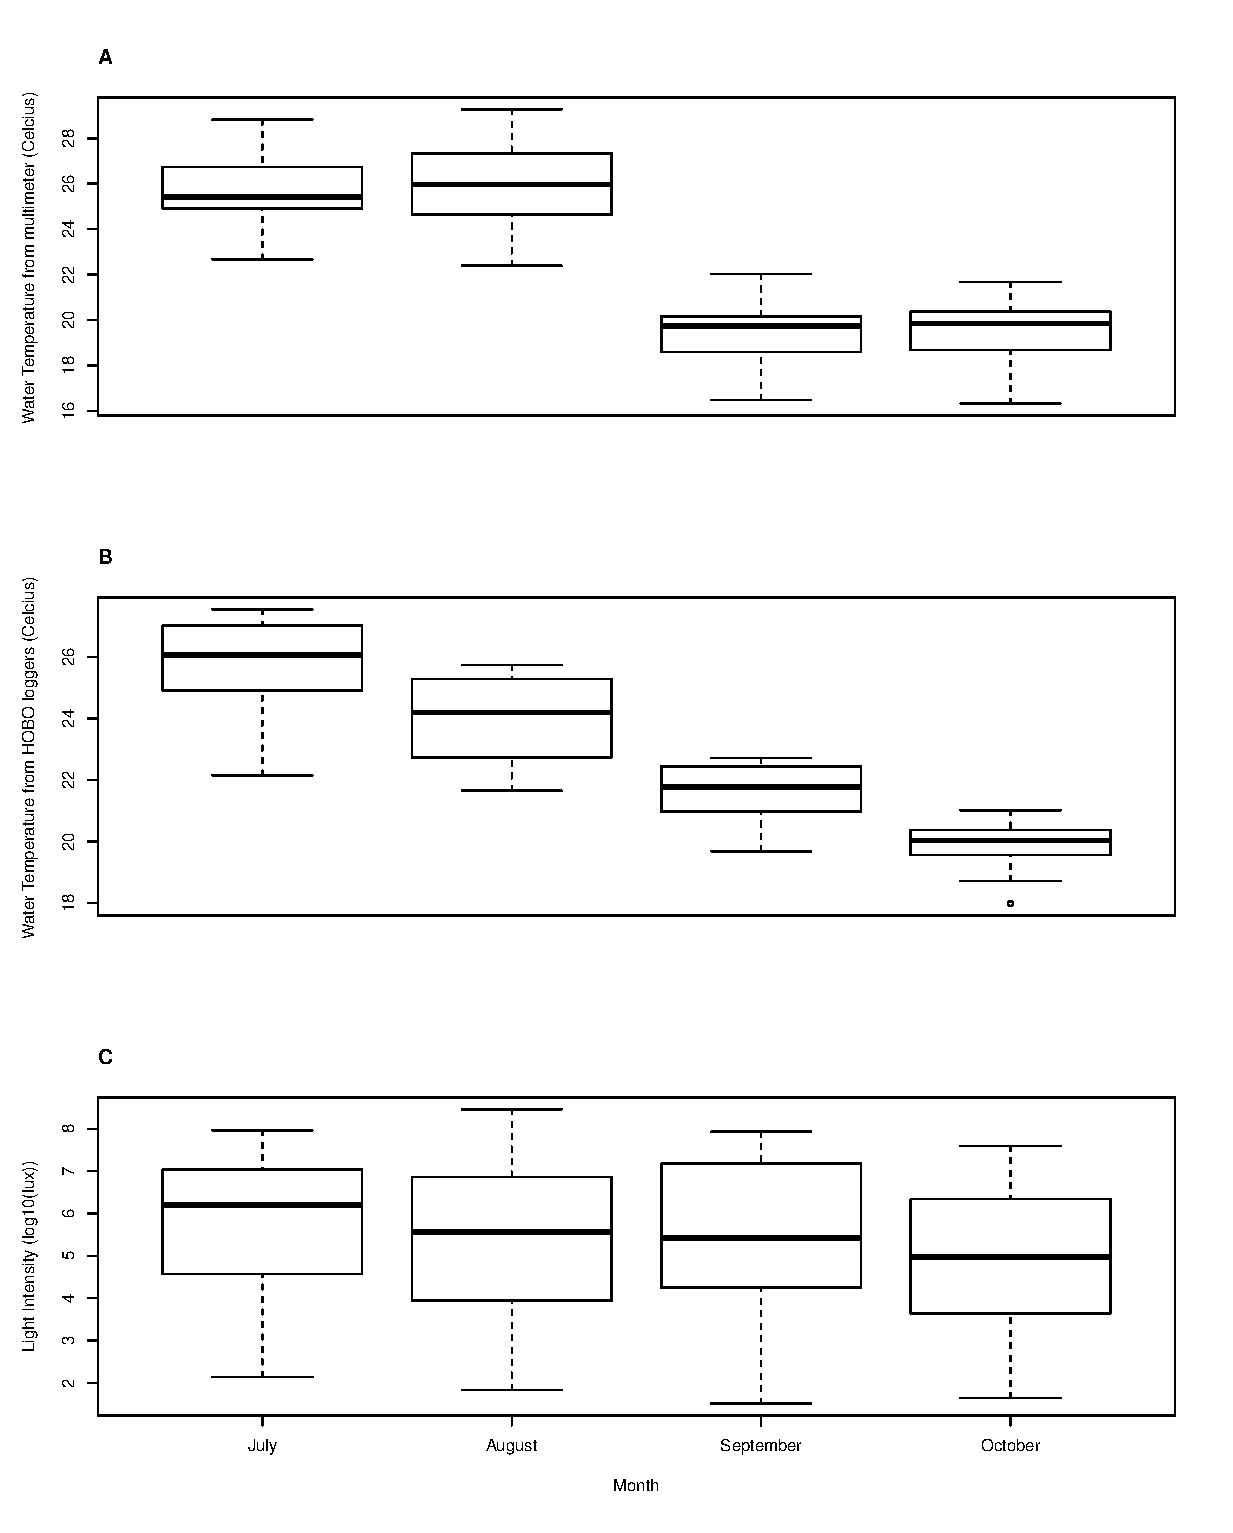
\includegraphics[width=\textwidth]{figures/hobo}
\caption{
(A): Boxplot summary of the average lake temperature measured at the time of sampling with hand-held multimeter 
(B): Boxplot summary of average lake temprature from HOBO loggers. 
(C): Boxplot summary of light intensity also measured by HOBO loggers.
} 
\label{fig:hobo}
\end{figure}


\begin{figure}[!h]
 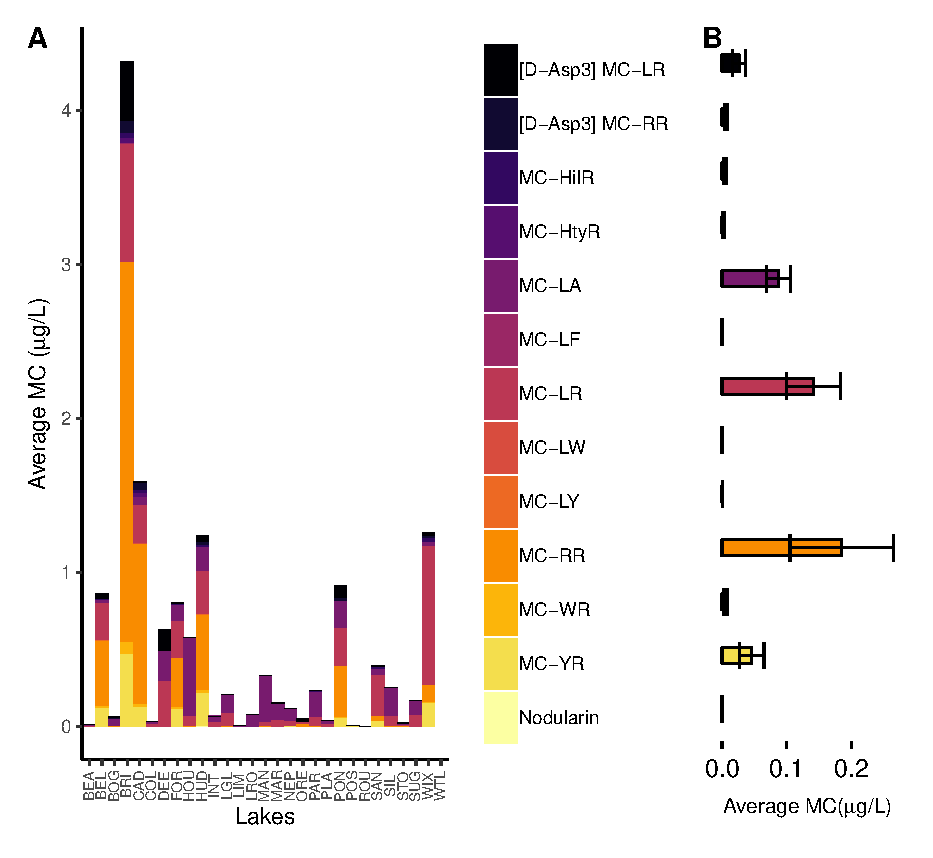
\includegraphics[width=\textwidth]{figures/congenerbar}
 \caption{
 (A): Average MC found at each lake in all four months. The height of each bar represents the total average of MC. The proportion of each congener is represented by color in each bar  
(B): Average MC congener with the included error bars represents one standard deviation of the mean}
 \label{fig:congenerbar}
\end{figure}



\begin{figure}[!ht]
\vspace*{-15mm}
\scalebox{1.0}{
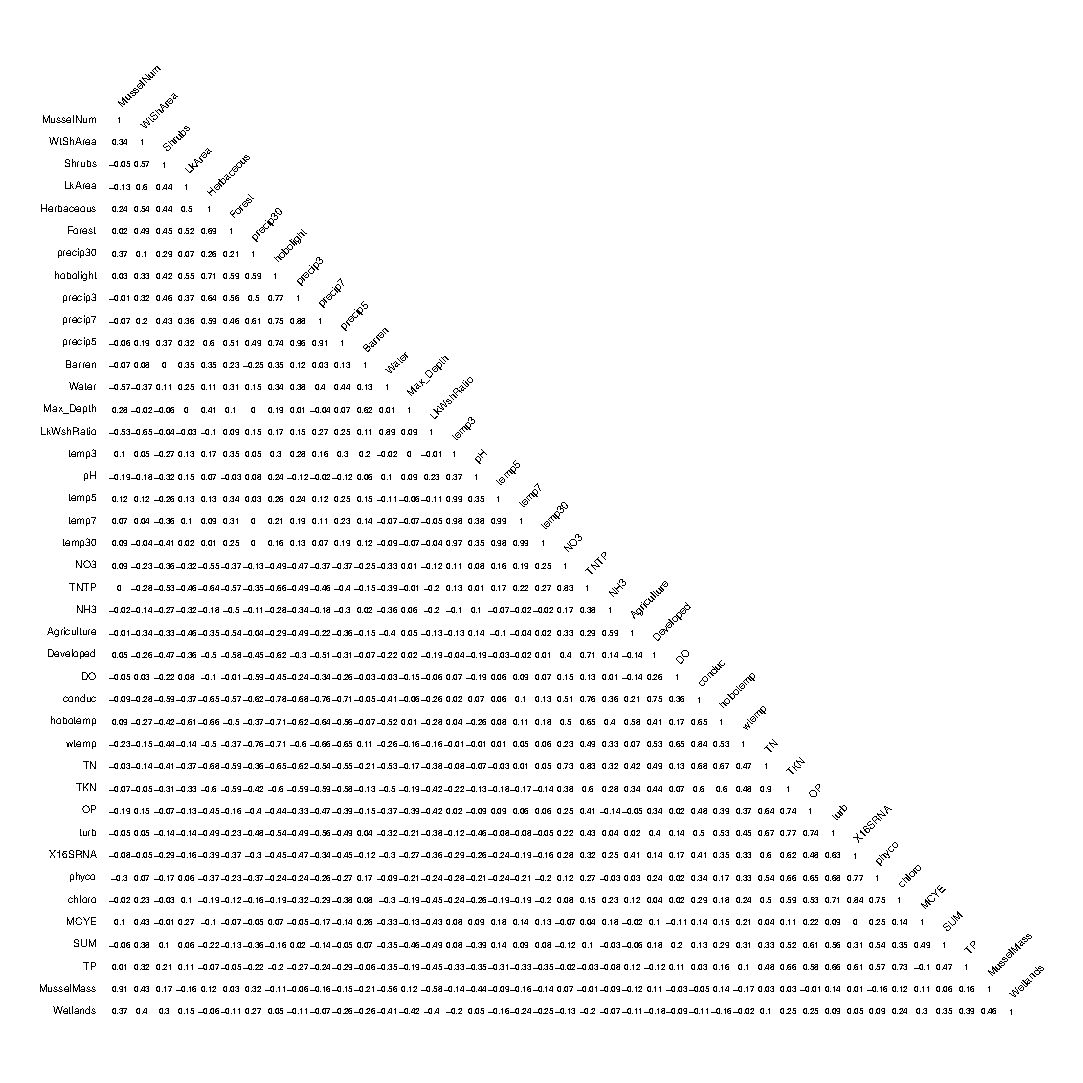
\includegraphics[width=1.1\textwidth,height=1.1\textheight]{figures/matrixfull}}
\vspace*{-15mm}
\caption{Correlation matrix displaying Pearson's coefficient on the full data.}
\label{fig:matrixfull}
\end{figure}


\begin{figure}[!hp]
\centering
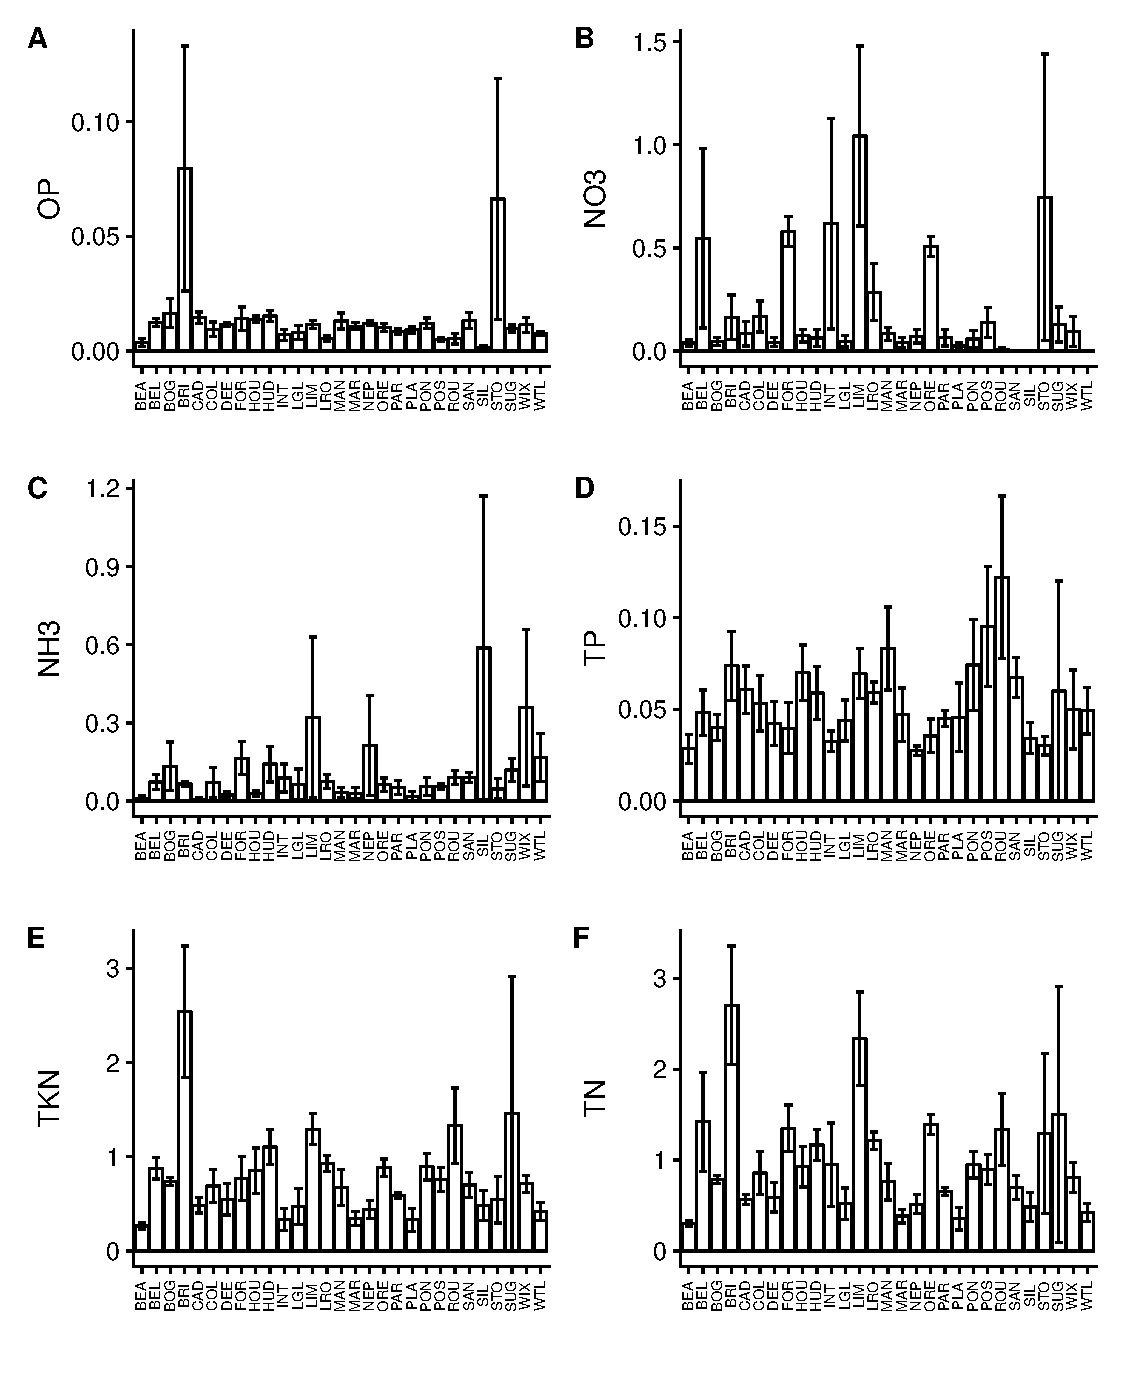
\includegraphics[width=\textwidth]{figures/nutboxplotlake}
\caption{Average nutrient concentrations for each lake for all of summer 2017. Figure (A): Orthophosphate (mg-P/L). Figure (B): Nitrate+nitrite (mg-N/L). Figure (C): Ammonia (mg-N/L). Figure (D): Total phosphorus (mg-P/L). Figure (E): Total Kjeldahl nitrogen (mg-N/L). Error bars represents one standard deviation of the mean. }
\label{fig:nutrients}
\end{figure}


\begin{figure}[!hp]
\centering
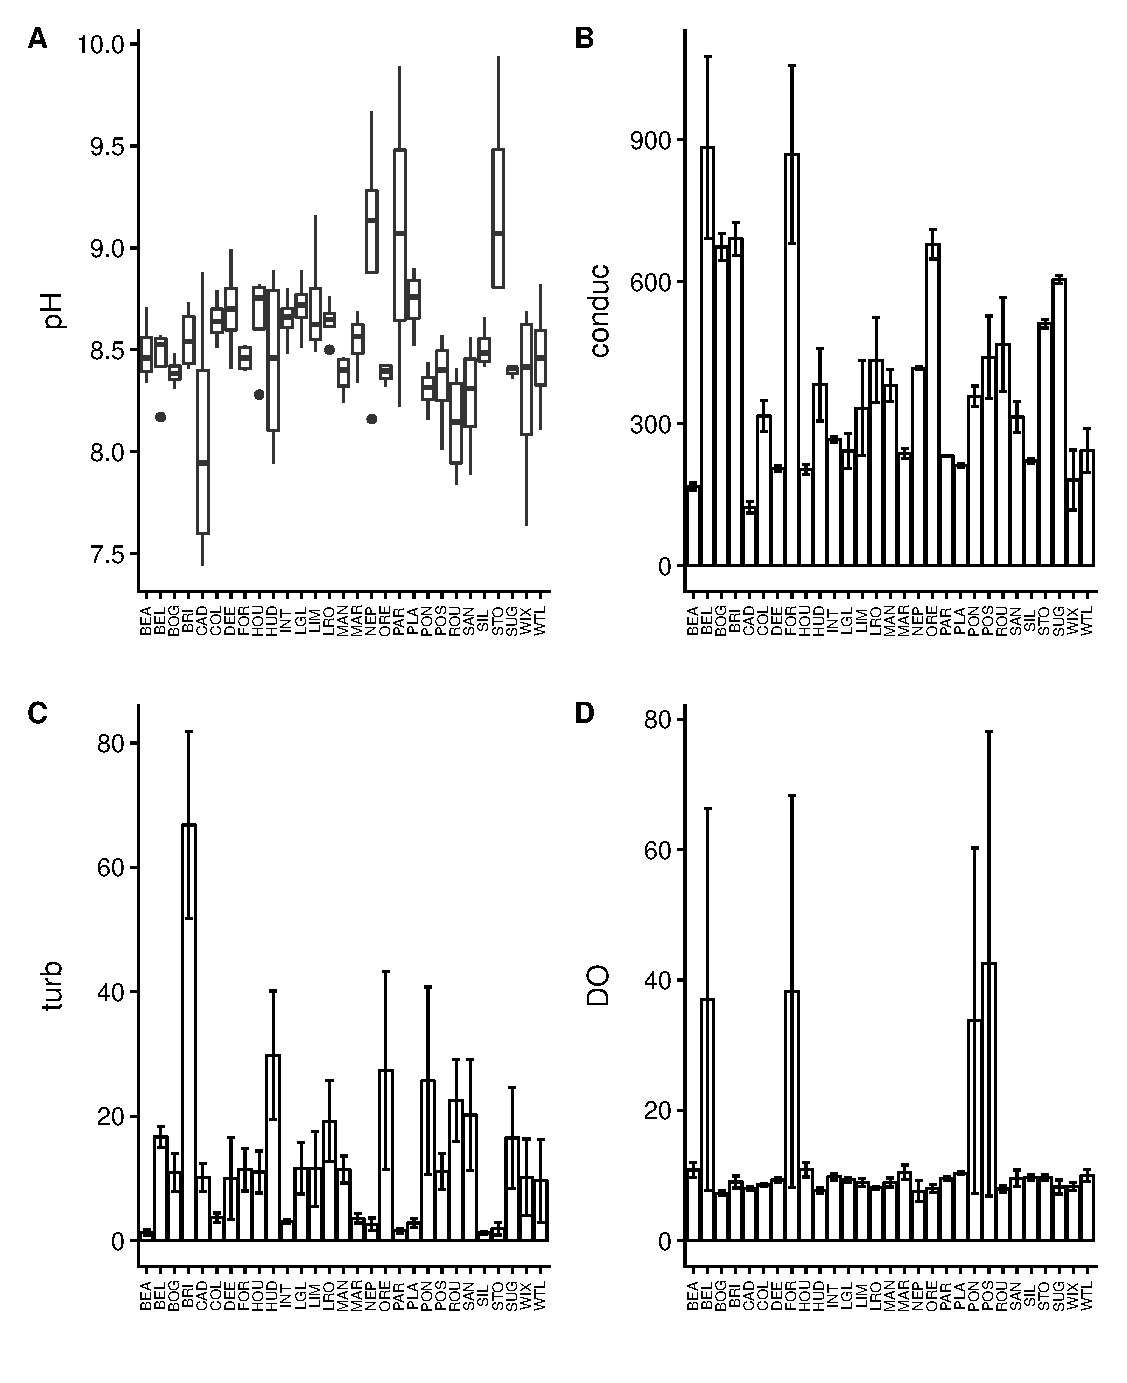
\includegraphics[width=\textwidth]{figures/watboxplotlake.eps}
\caption{Summary of measured water chemical parameters. Figure (A): A box and whisker plot of pH. Figure (B): Bar plots of average conductance. Figure (C): Average turbidity. Figure(D): Average dissolved oxygen. }
  \end{figure}

%
\section*{SPATTs}
Solid Phase Adsorption Toxin Tracking (SPATTs) is new unique method of monitoring waterbodies. A Nitex mesh bag containing HP-20 resin (styrene-divinylbenzene copolymer) is submerged in waterbody of interest for a period of time. During this period, free-floating compounds will adsorb onto the polymer beads. SPATTs can are then retrieved and analyzed for chemical analytes of interest. This technique can be useful if sampling frequency is financially limited..





\section*{Methods}

A 1 meter x 5 centimeter strip of Nitex mesh were precisionaly cut. The Nitex strip was sewn by folding half lenth-wise (or \emph{hot dog} style). With tape holding the fold, the end of the strip was sewn 0.5cm from the edge. Stiching design was tight to ensure no leakage of polymer beads.

9-10cm of sewn Nitex strips were cut and zip-tied about 0.5cm at one end. 3.00-3.01 grams of HP-20 resin was filled using a funnel. The other end is zip-tied once the Nitex bag is full. SPATT bags are activated by soaking in 100\% methanol for 24 hours under $4^\circ$C. Next the SPATTs were rinsed with Milli-Q water and then soaked for 24 hours in Milli-Q water under $4^\circ$C before deploying the SPATTs bag in our target sample lakes.

At each lake site, two SPATT bags were loaded into a slotted PVC pipe. At each lake, a float was installed as described in section \ref{sampling}. SPATTs are left for about a month at each lake. When SPATTs are retrieved, they are carefully removed and rinsed with Milli-Q water and stored in a 15mL centrifuge vial with a plastic spacer on the bottom. SPATTs are stored at $4^\circ$ during transport back to the lab. The SPATTs are centrifuged at 8000rpm. The spacer allows liquid to pool on the bottom when centrifuged. When centrifuged, the SPATT bags are cut open and the resin is poured into a 50mL centrifuge tube. Milli-Q water is used to rinse the SPATT bags to effectivly transfer all the resin. About 30mL of Milli-Q water is used. The solution is allowed to rest so the resin settles to the bottom. Using a pipet, the water is carefully decanted until the total volume is 5mL.  A solution of 80\% methanol with 10$\mu$M ammonium formate is added to the tube until the total volume is 50mL. The solution is gently mixed and then allowed to settle for 30 minutes.

\section*{Results}

Out of all 12 congeners, MC-LA, MC-LR, and MC-RR were the most frequently detected congener.

\begin{table}[!ht]
\centering
  \caption*{Microcystin Congener from SPATTs}
  \label{}
\begin{tabular}{@{\extracolsep{5pt}}lccccc}
\\[-1.8ex]\hline
\hline \\[-1.8ex]
Statistic & \multicolumn{1}{c}{N} & \multicolumn{1}{c}{Mean} & \multicolumn{1}{c}{St. Dev.} & \multicolumn{1}{c}{Min} & \multicolumn{1}{c}{Max} \\
\hline \\[-1.8ex]
{[D-Asp3]}MC-RR & 91 & ND & ND & ND & ND \\
MC-RR & 91 & 164 & 1,116 & ND & 10,380 \\
Nodularin & 91 & 2 & 17 & ND & 160 \\
MC-YR & 91 & 10 & 30 & ND & 145 \\
MC-HtyR & 91 & 0 & 2 & ND & 18 \\
MC-LR & 91 & 353 & 1,211 & ND & 8,146 \\
{[D-Asp3]}MC-LR & 91 & 2 & 10 & ND & 92 \\
MC-HilR & 91 & 1 & 6 & ND & 53 \\
MC-WR & 91 & 0 & 1 & ND & 7 \\
MC-LA & 91 & 534 & 2,063 & ND & 13,977 \\
MC-LY & 91 & 1 & 11 & ND & 101 \\
MC-LW & 91 & 0 & 0 & ND & 0 \\
MC-LF & 91 & 0 & 2 & ND & 18 \\
Total MC & 91 & 1,066 & 3,273 & ND & 22,124 \\
\hline \\[-1.8ex]
\multicolumn{6}{r}{Values are expressed as (ng of MC / gram of resin)} \\
\end{tabular}
\end{table}

\begin{figure}[!ht]
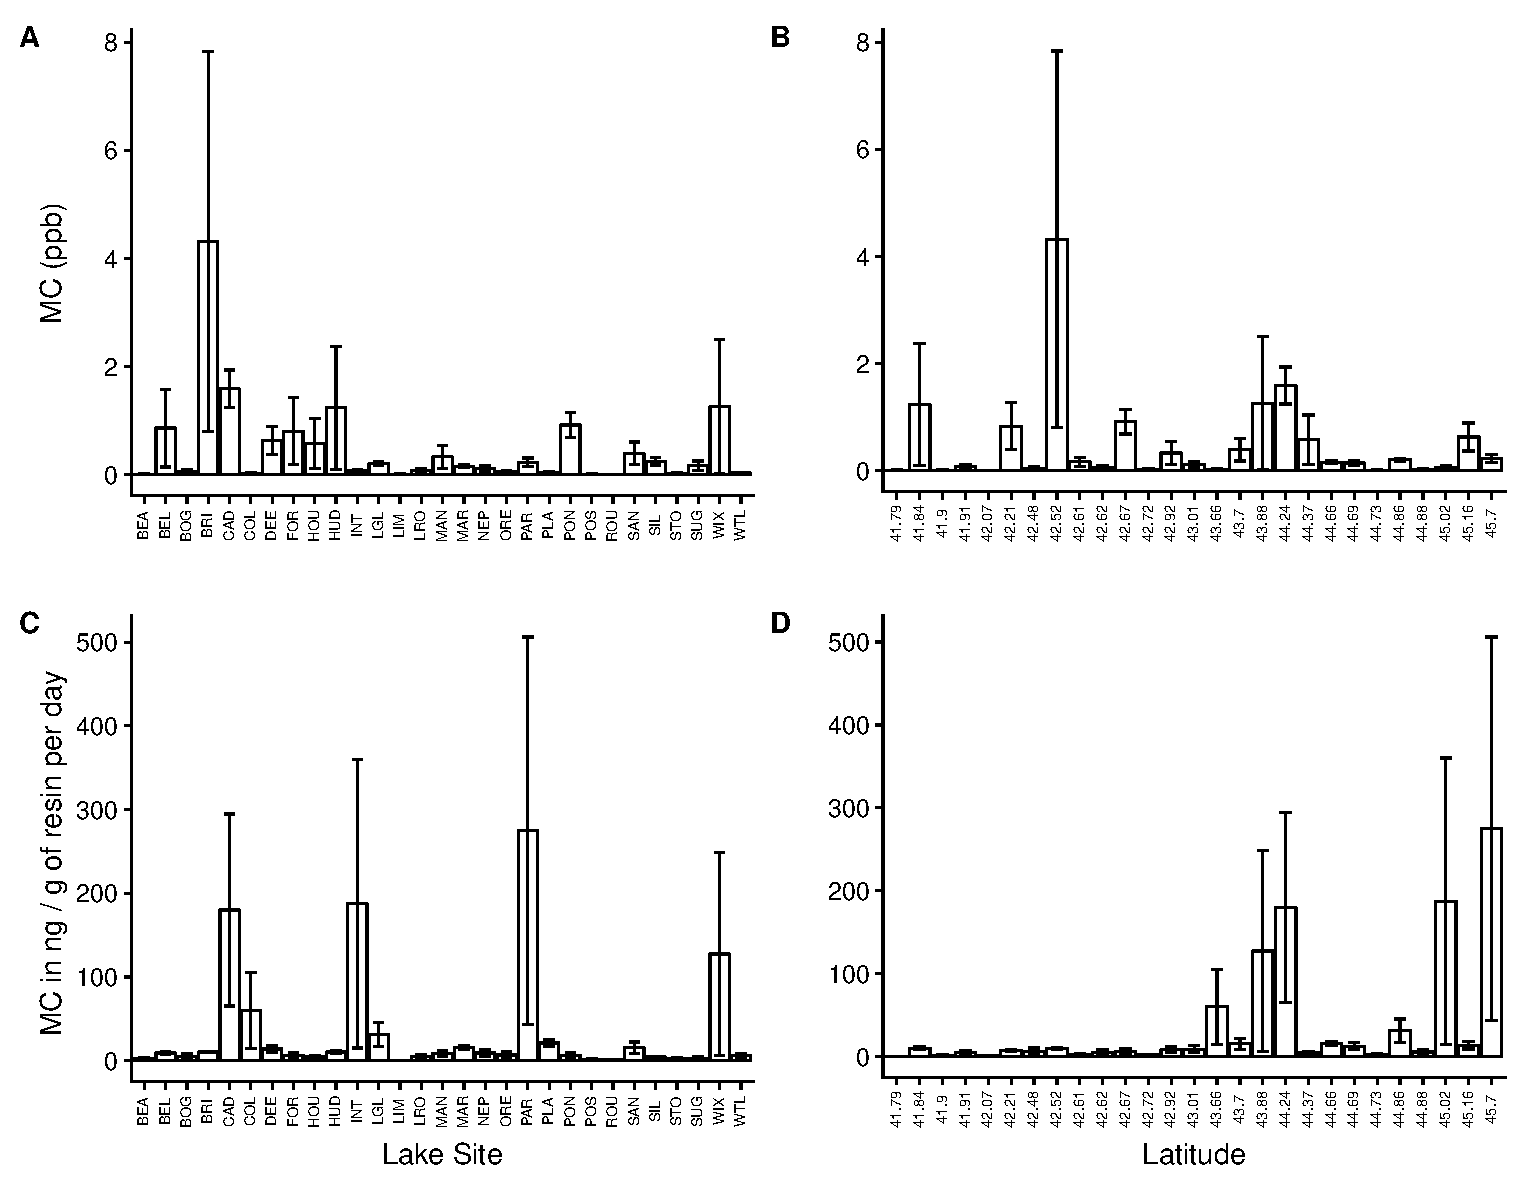
\includegraphics[width=\textwidth]{figures/spatttboxplotlake}
\label{spattbox}
\caption*{Comparitive Results of Microcystin Measured from SPATTS and Grab Samples}
A) B) C) D)
\end{figure}


\clearpage
\newpage

%\GrizzAppendix{Lake Atlas}


\begin{figure}[t]
\centerline{%
  \resizebox{\textwidth}{!}{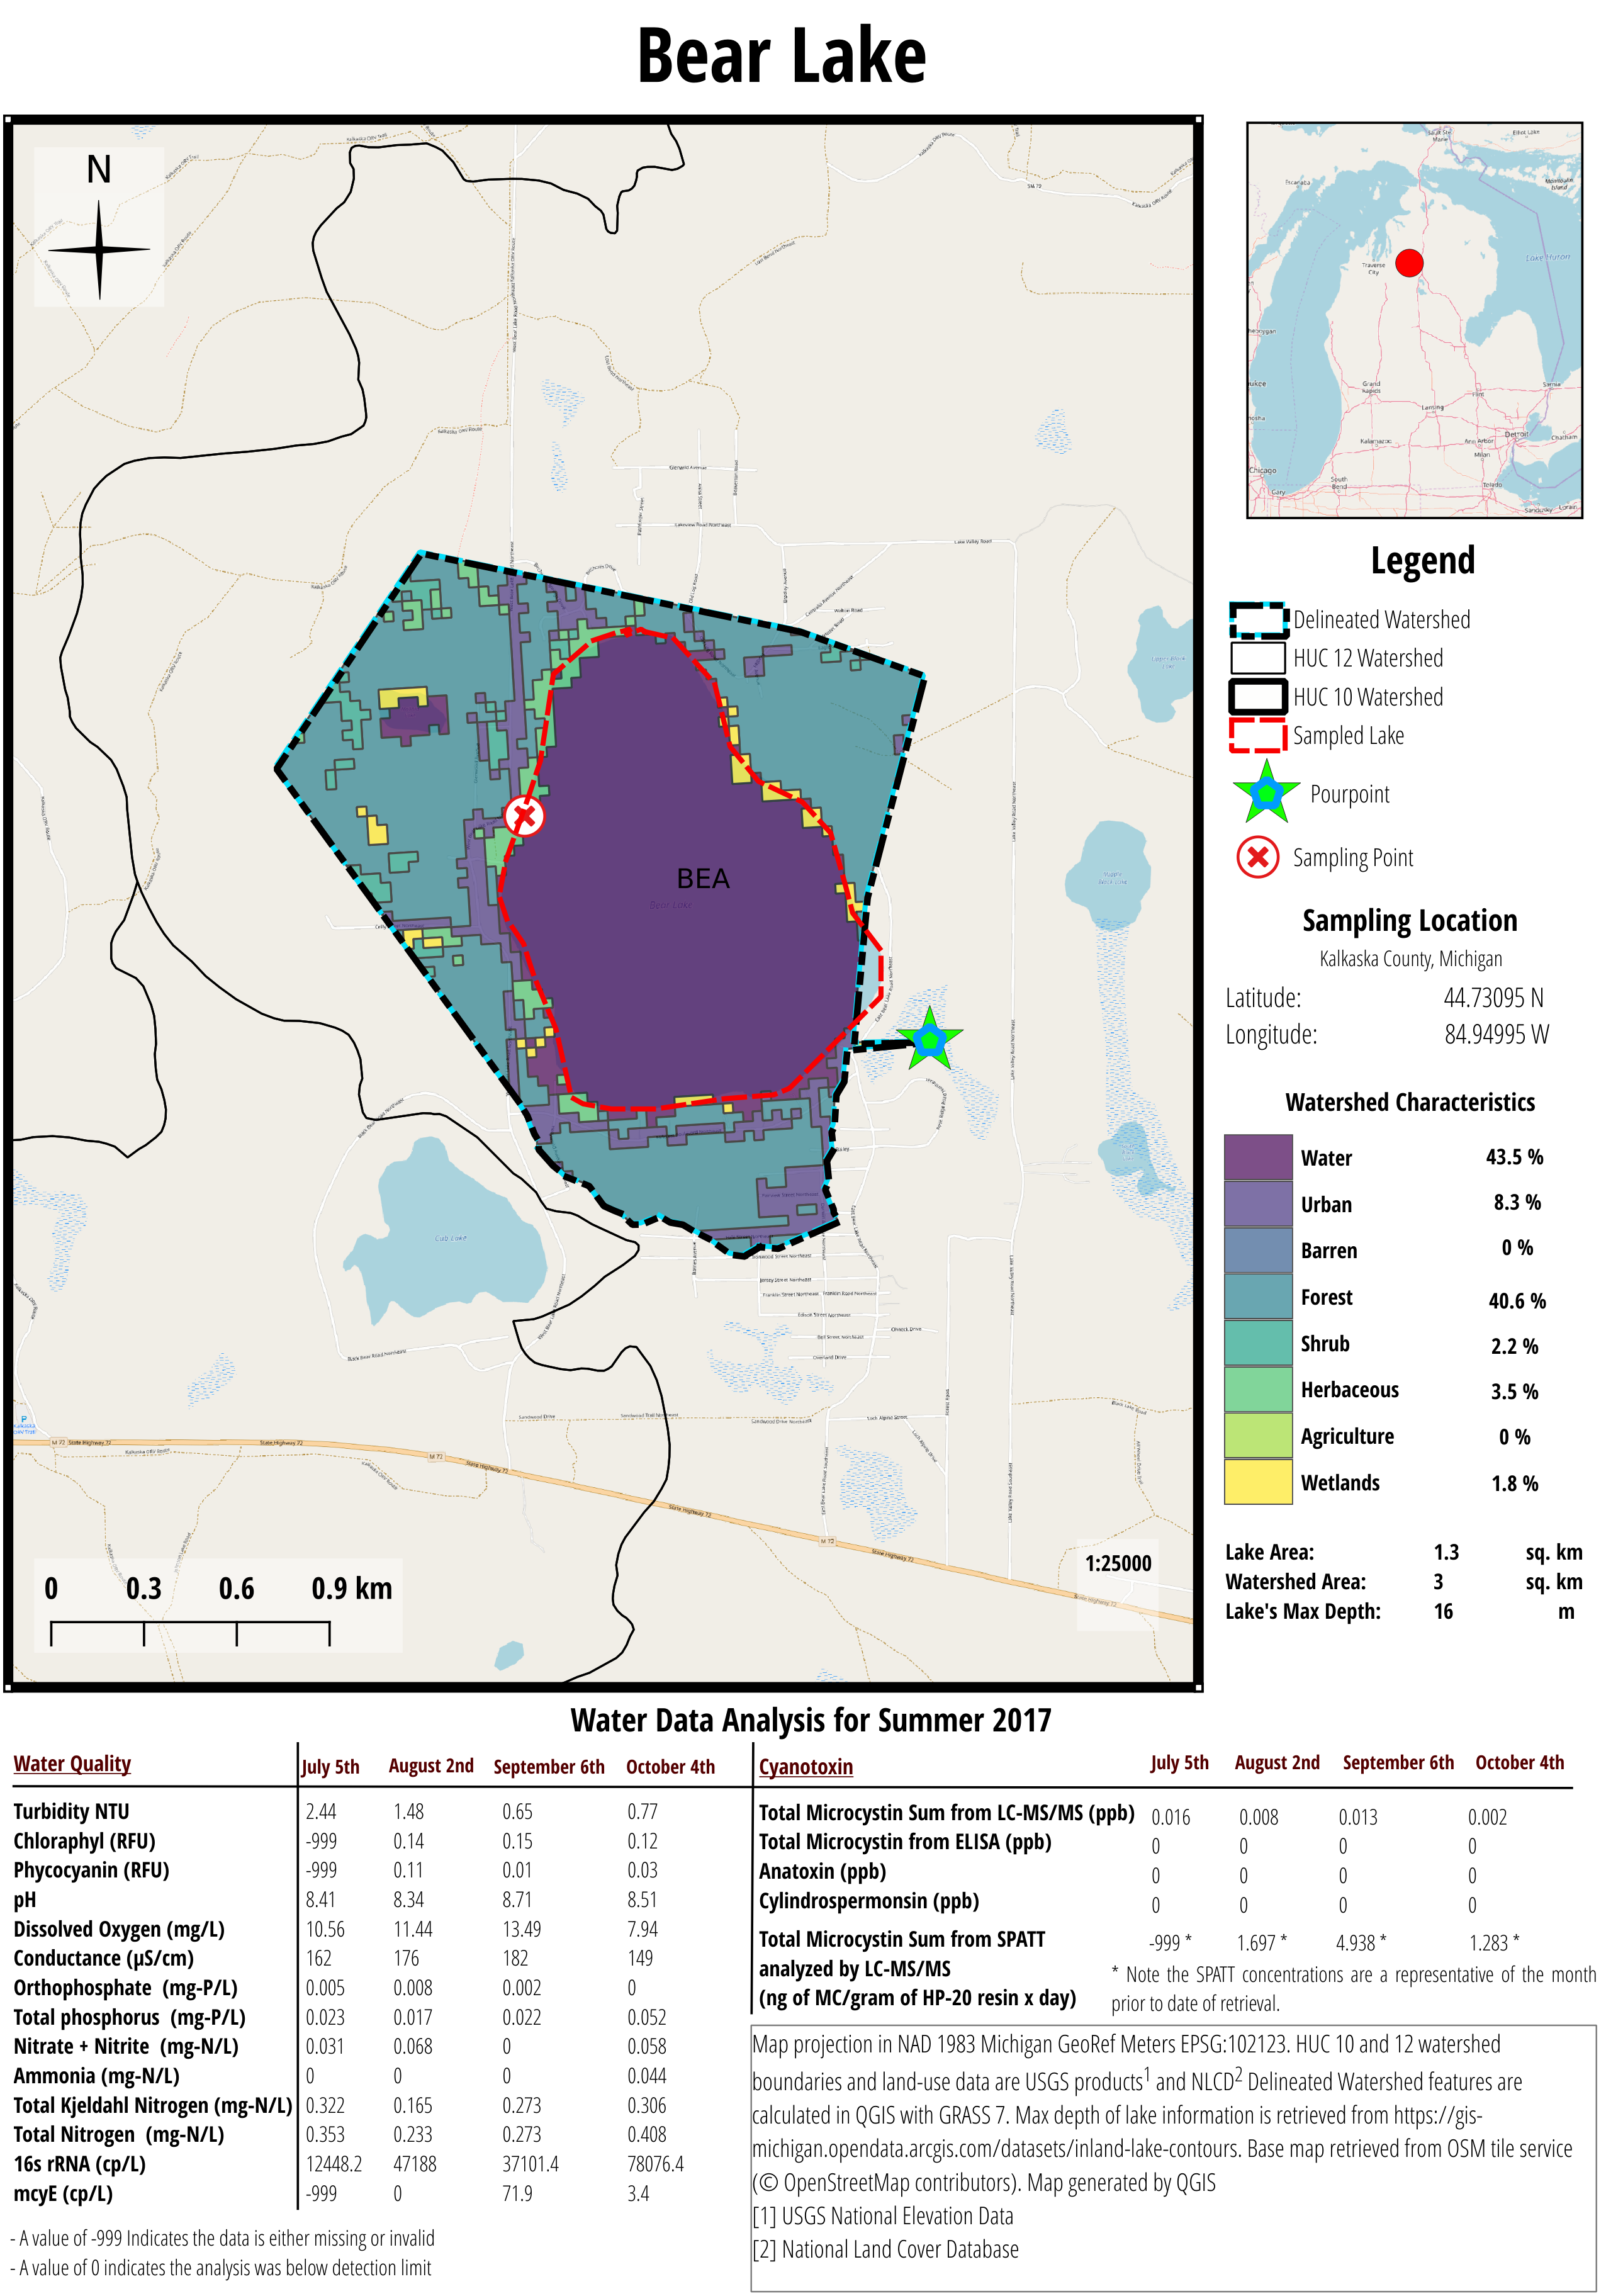
\includegraphics{figures/atlas/output_1}}
  }
\caption{GIS Map of Bear Lake}
\end{figure}

\begin{figure}[t]
\centerline{%
  \resizebox{\textwidth}{!}{\includegraphics{figures/atlas/output_2}}
  }
\caption{GIS Map of Belleville Lake}
\end{figure}

\begin{figure}[t]
\centerline{%
  \resizebox{\textwidth}{!}{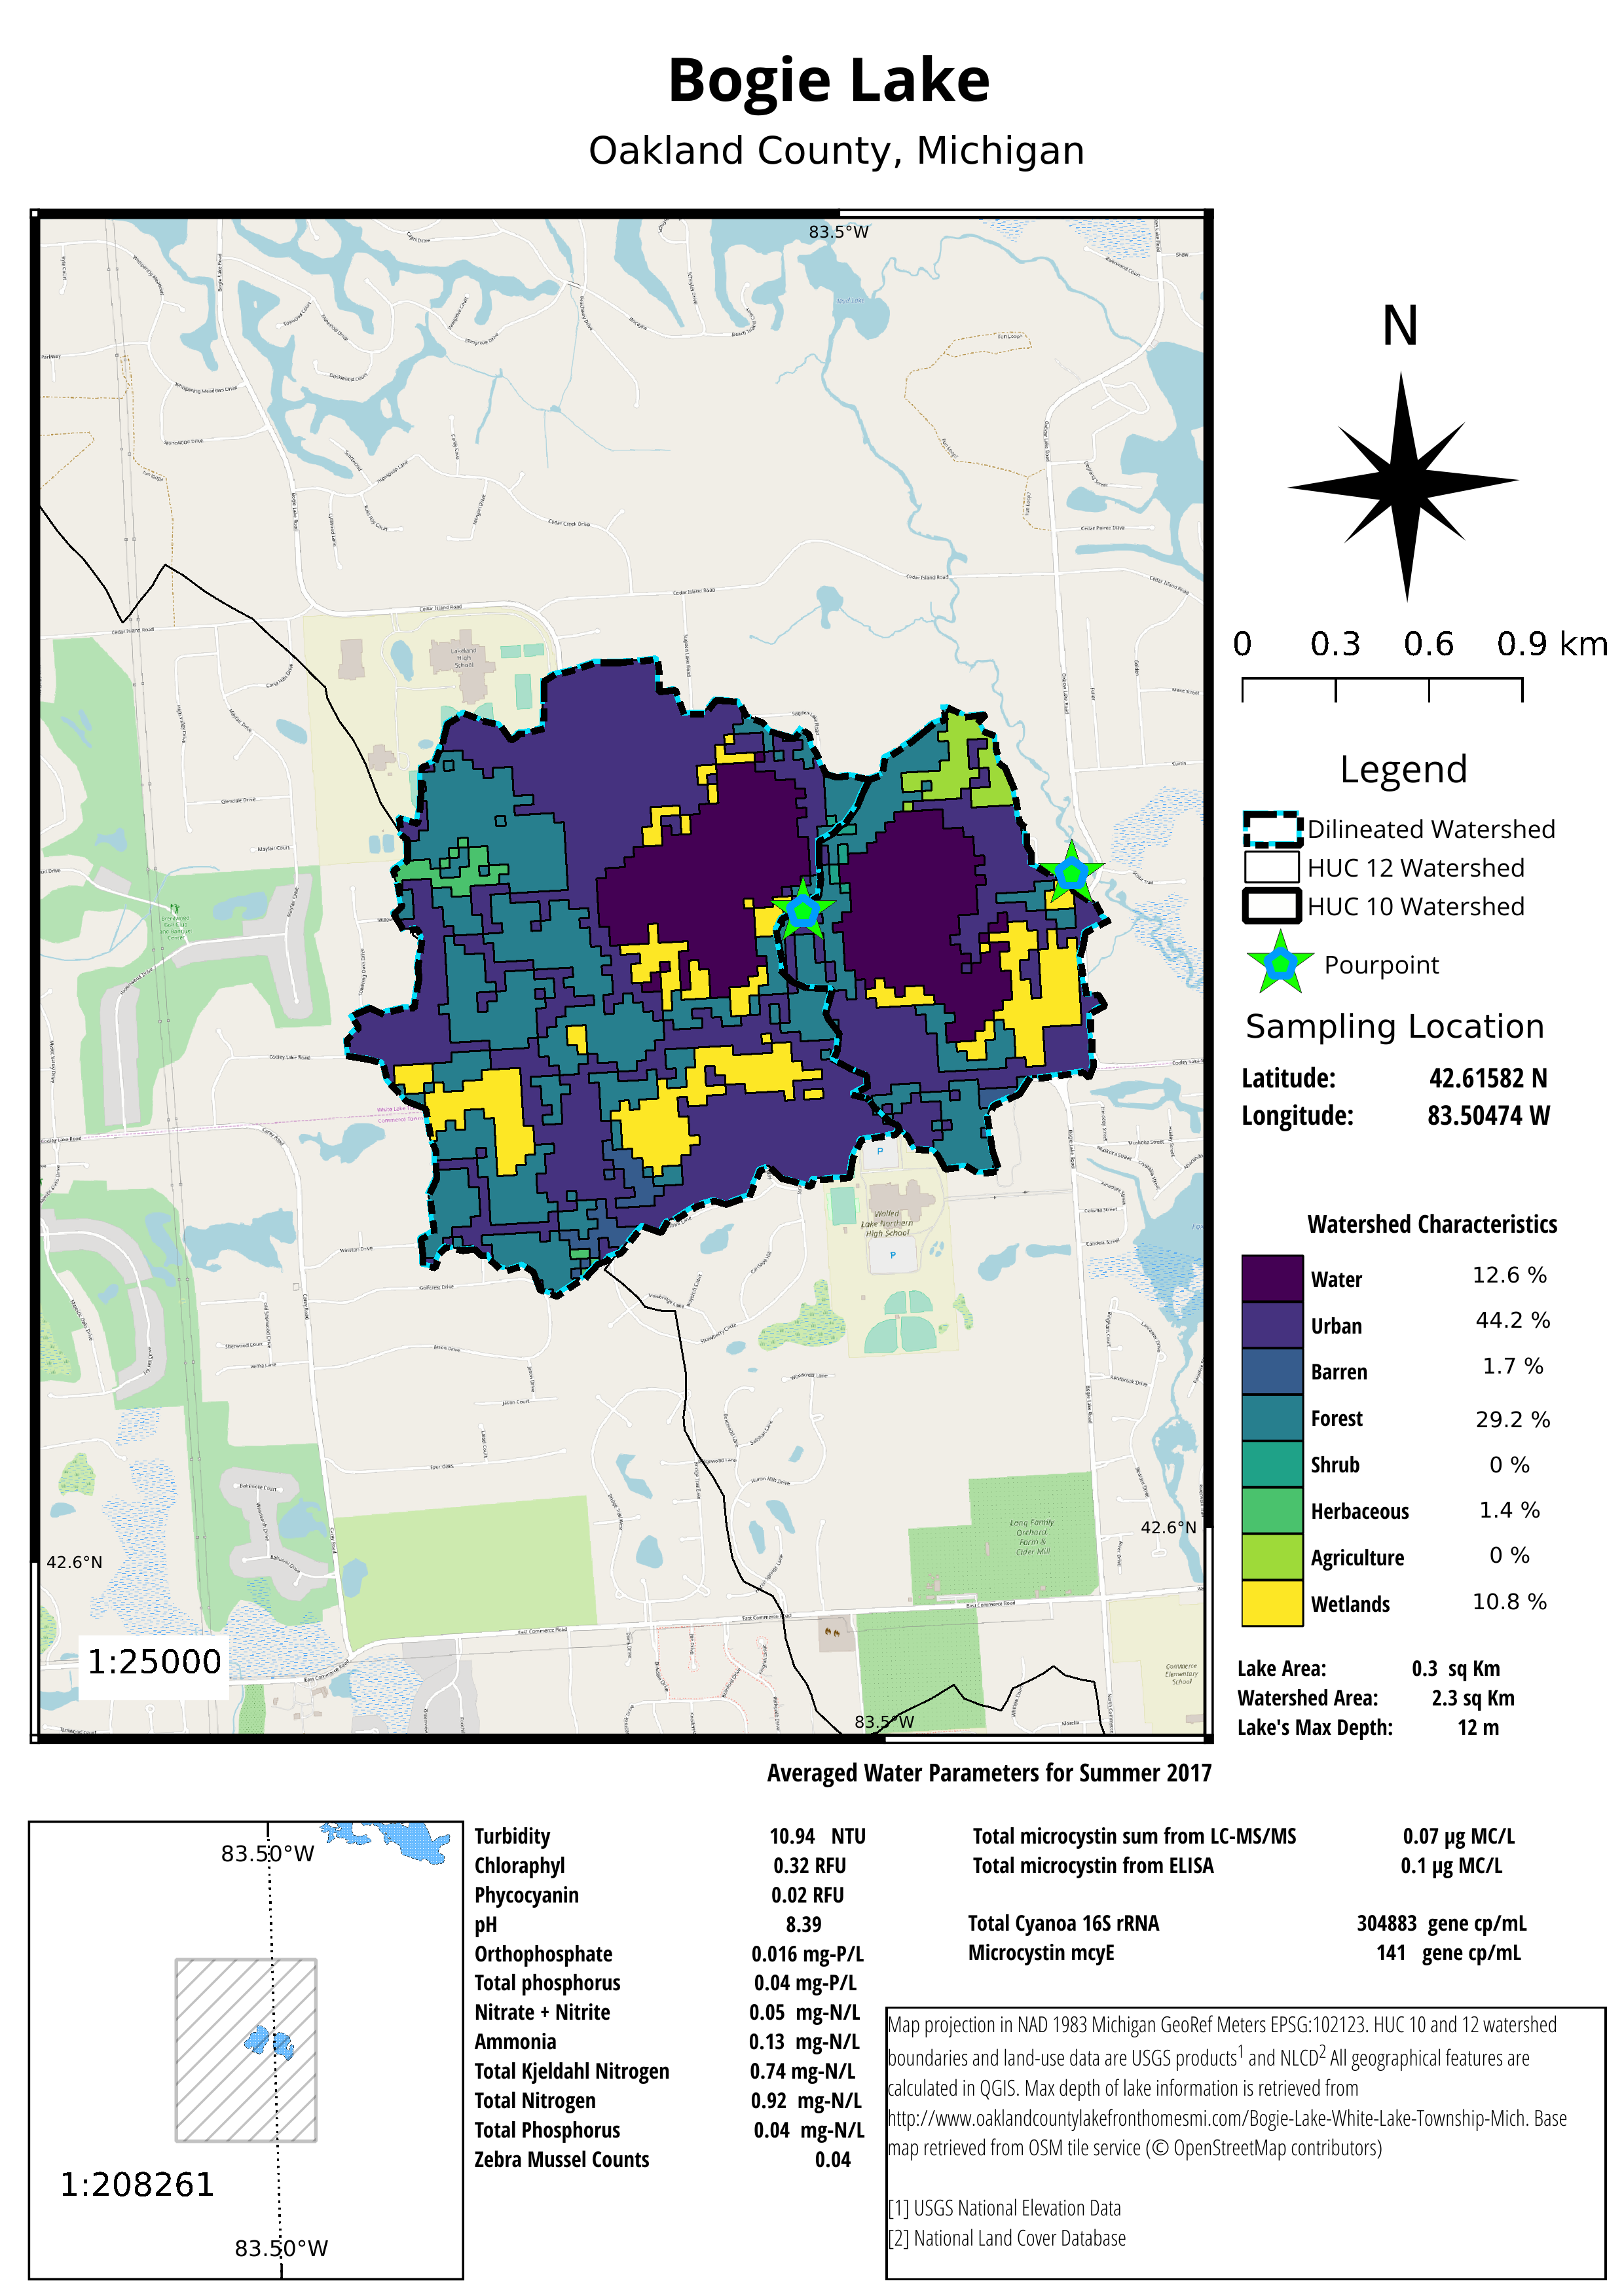
\includegraphics{figures/atlas/output_3}}
  }
\caption{GIS Map of Bogie Lake}
\end{figure}

\begin{figure}[t]
\centerline{%
  \resizebox{\textwidth}{!}{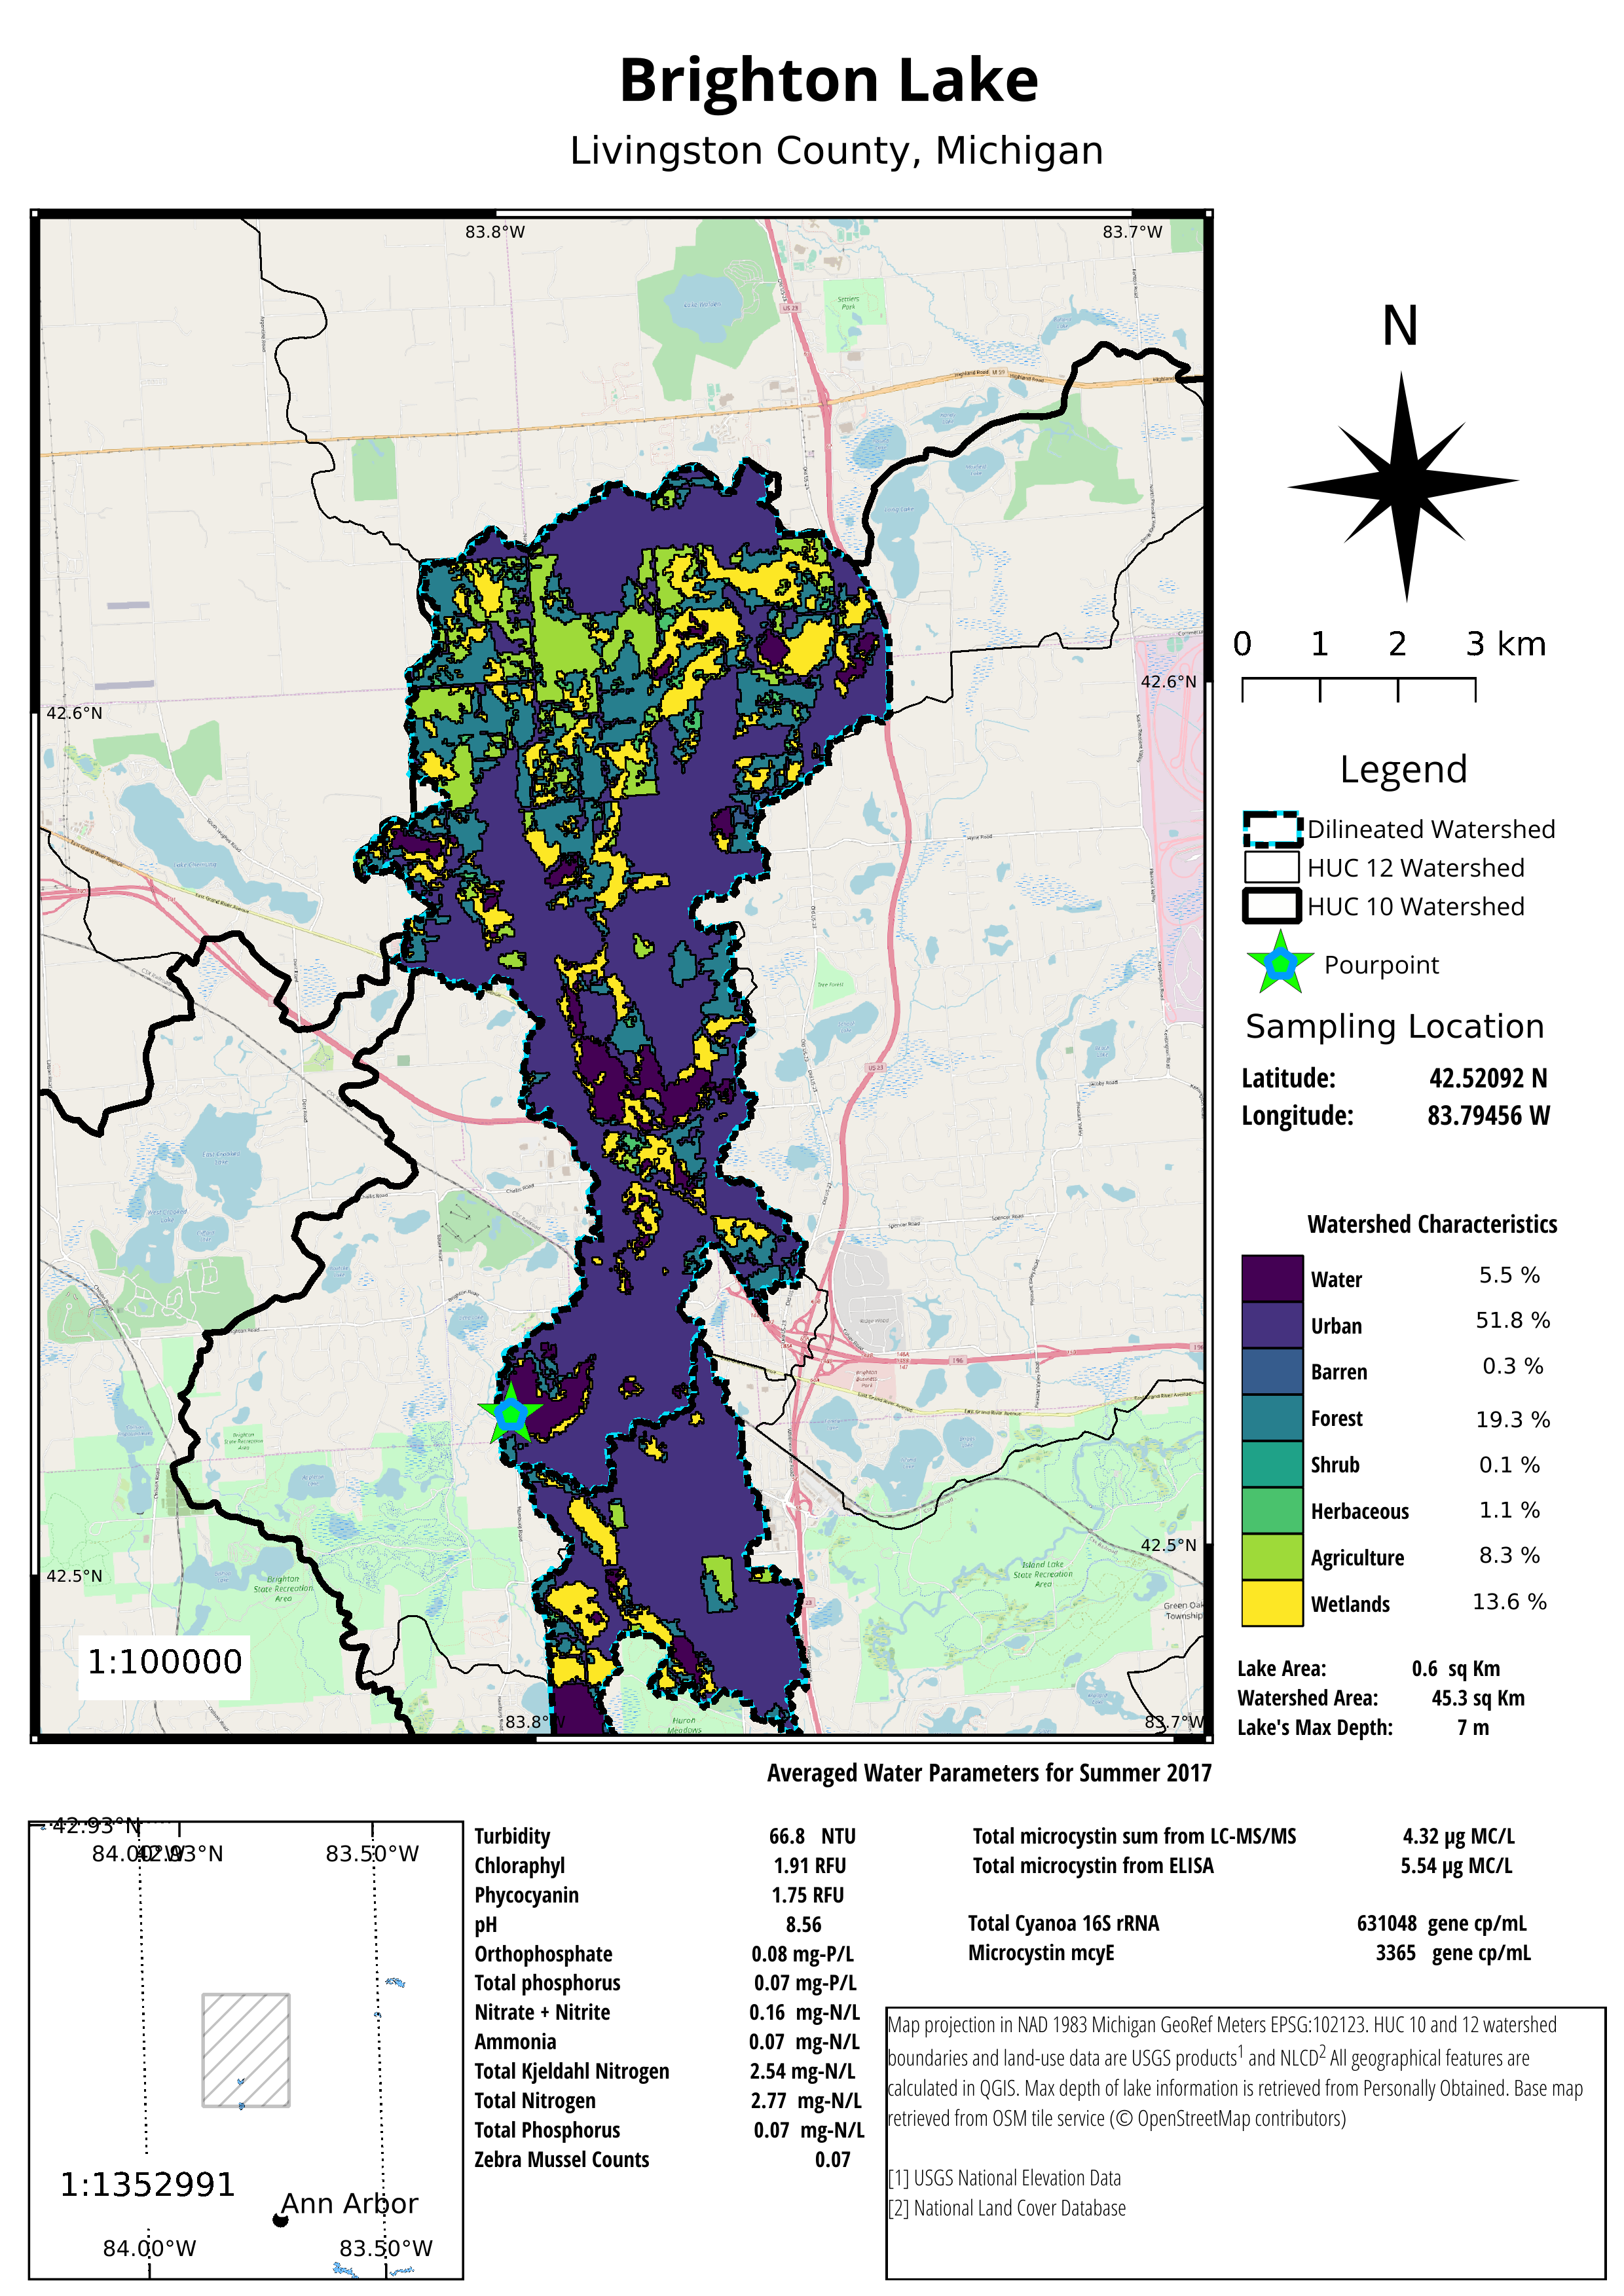
\includegraphics{figures/atlas/output_4}}
  }
\caption{GIS Map of Brighton Lake}
\end{figure}

\begin{figure}[t]
\centerline{%
  \resizebox{\textwidth}{!}{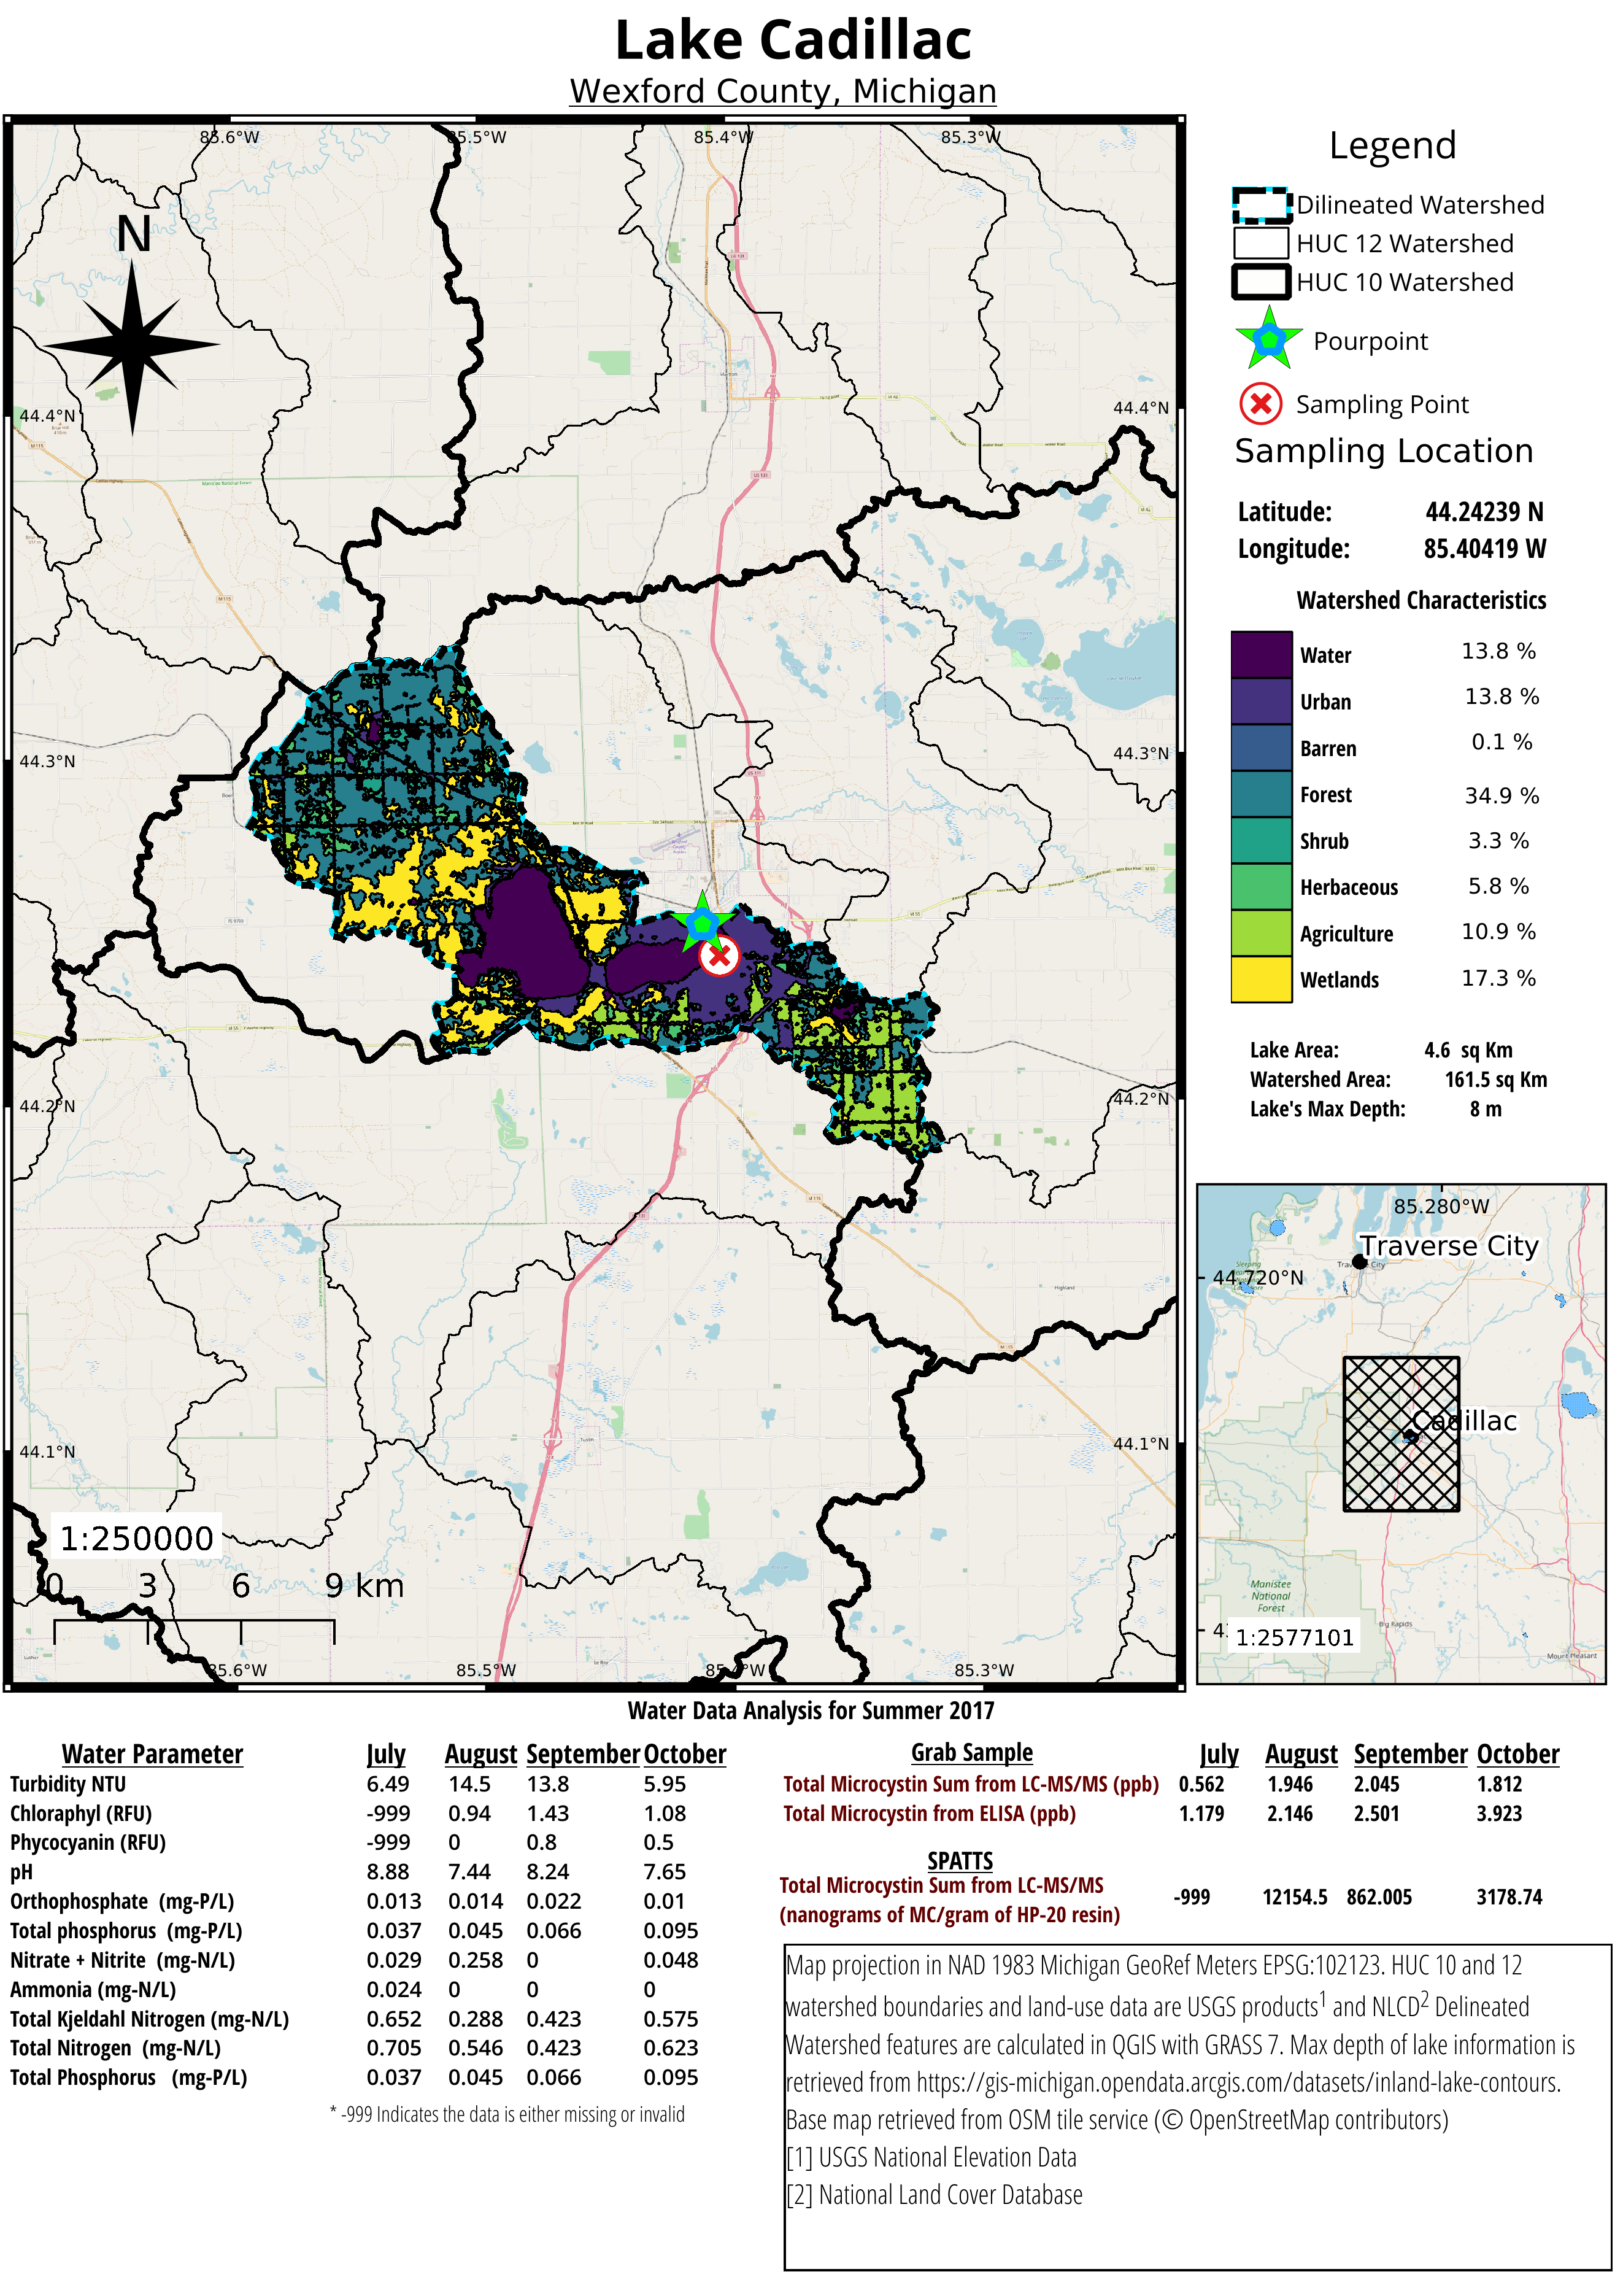
\includegraphics{figures/atlas/output_5}}
  }
\caption{GIS Map of Lake Cadillac}
\end{figure}

\begin{figure}[t]
\centerline{%
  \resizebox{\textwidth}{!}{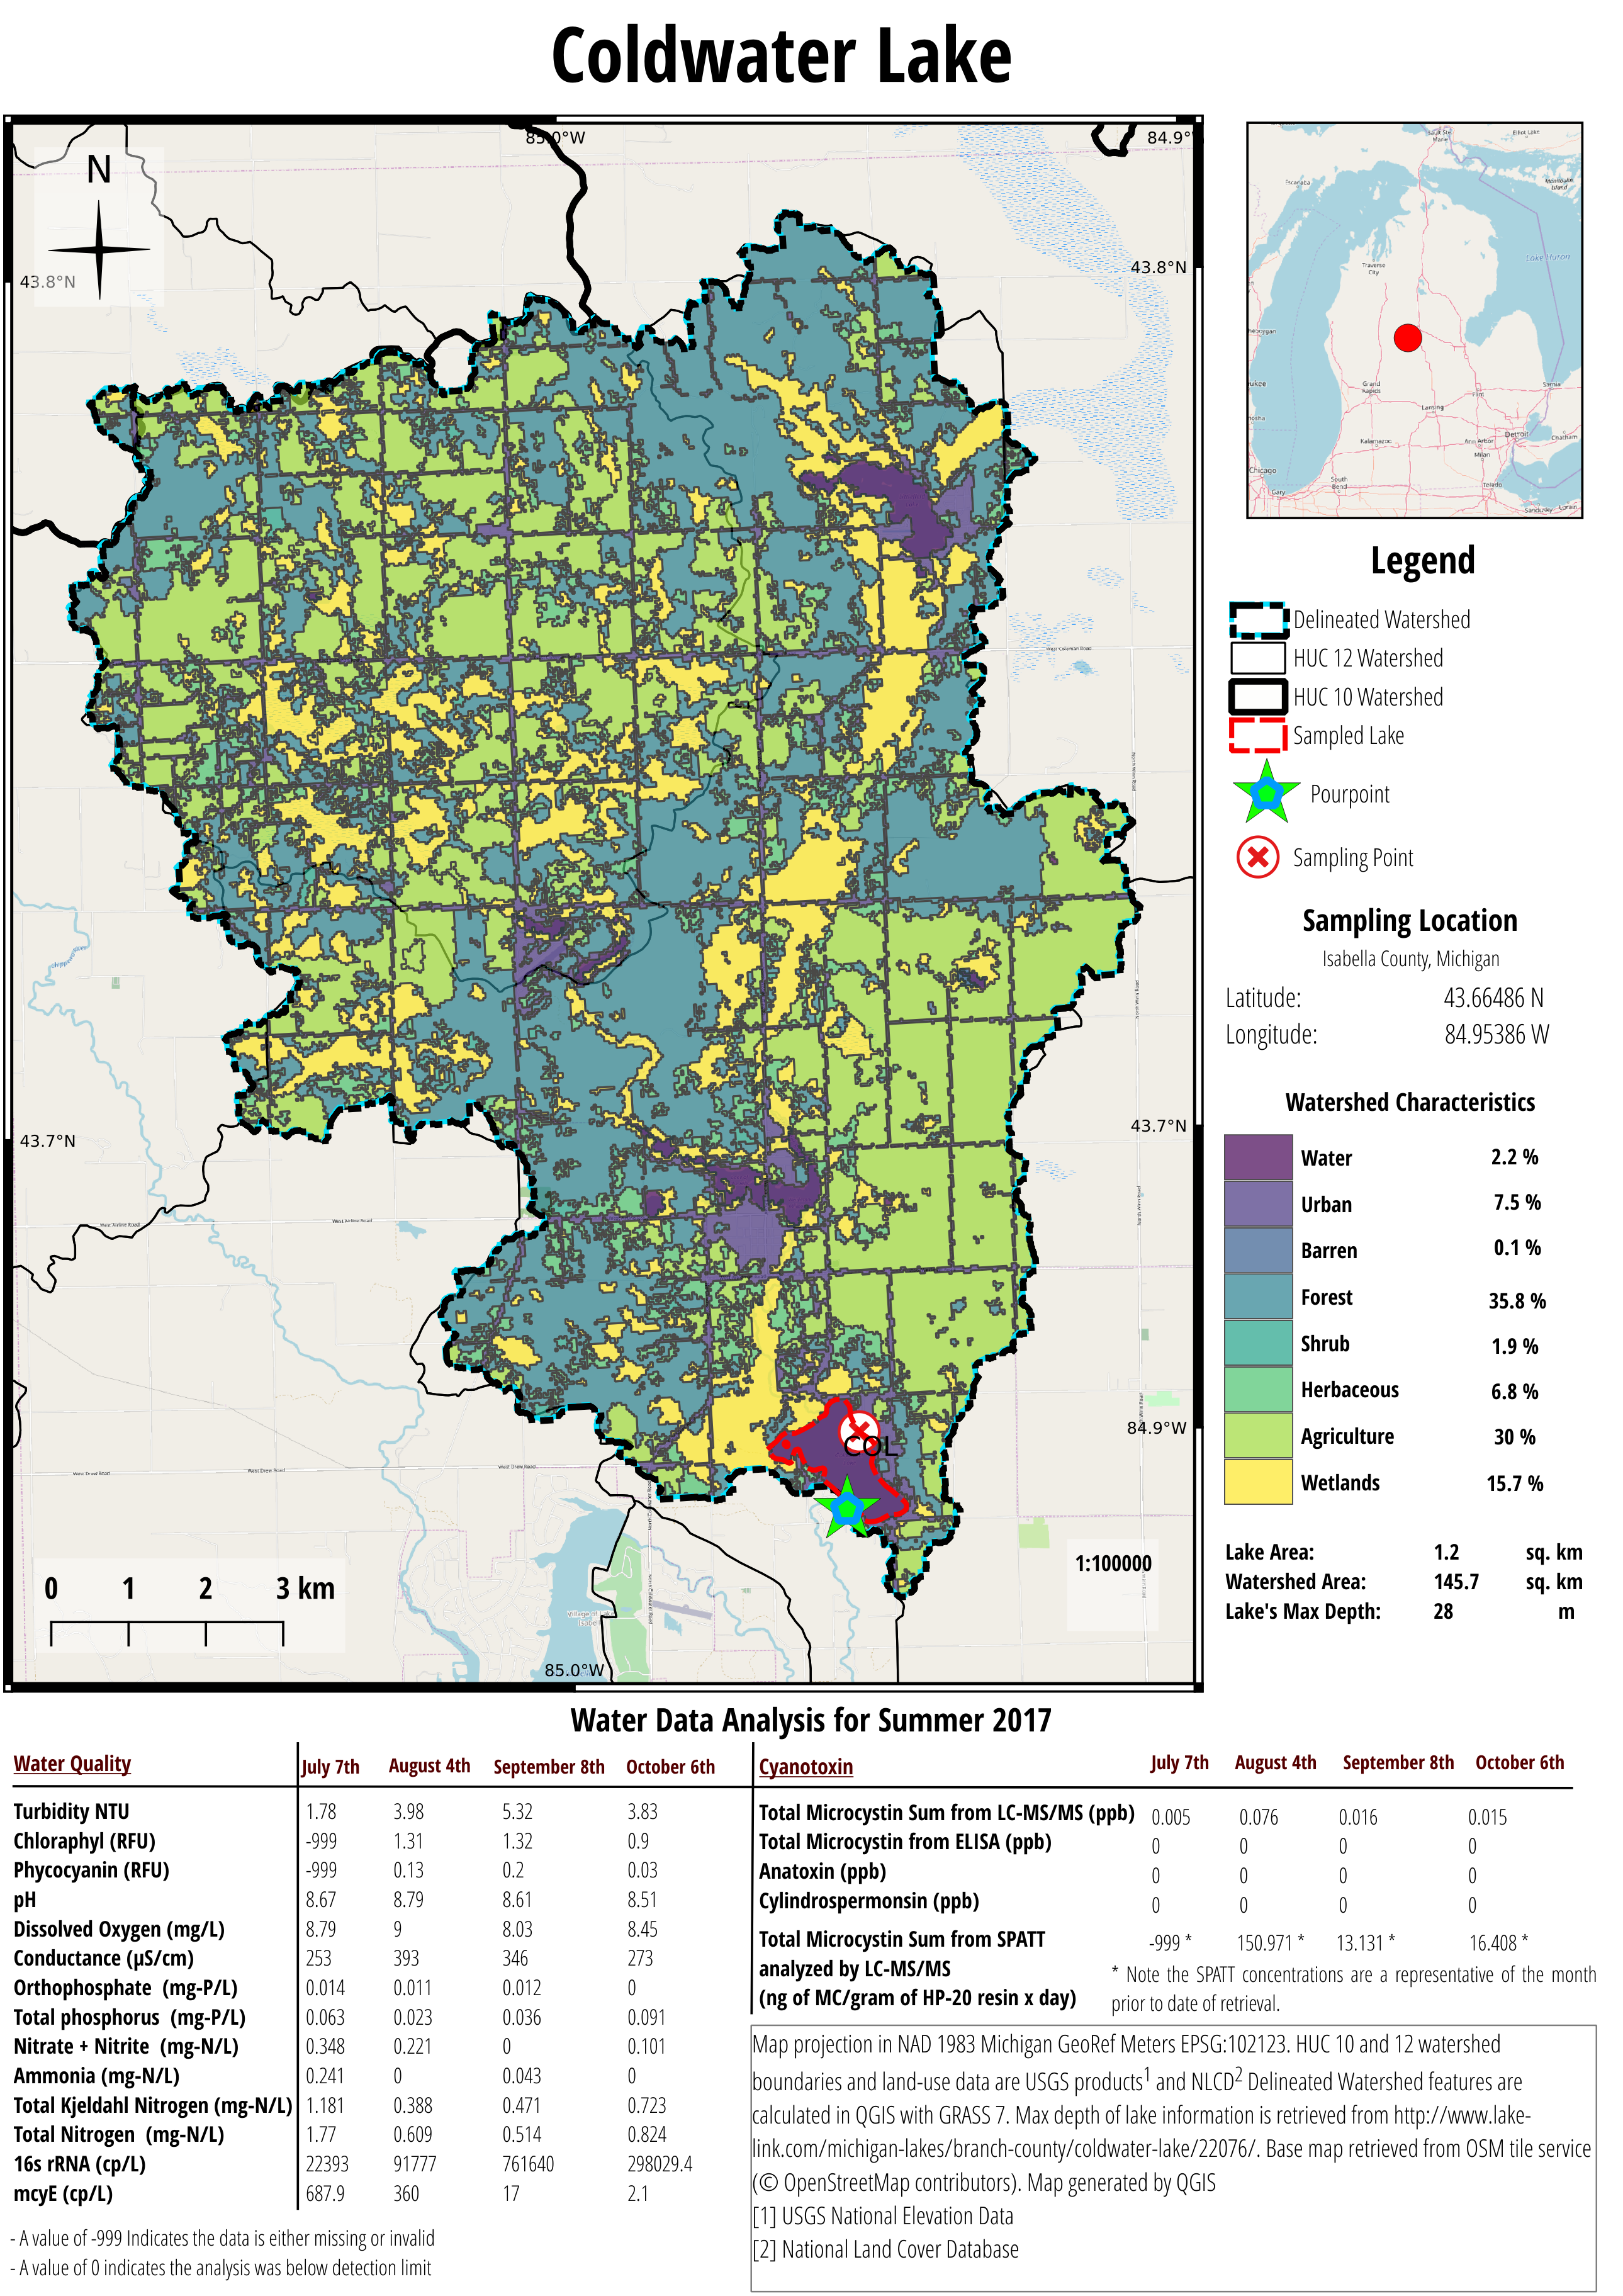
\includegraphics{figures/atlas/output_6}}
  }
\caption{GIS Map of Coldwater Lake}
\end{figure}

\begin{figure}[t]
\centerline{%
  \resizebox{\textwidth}{!}{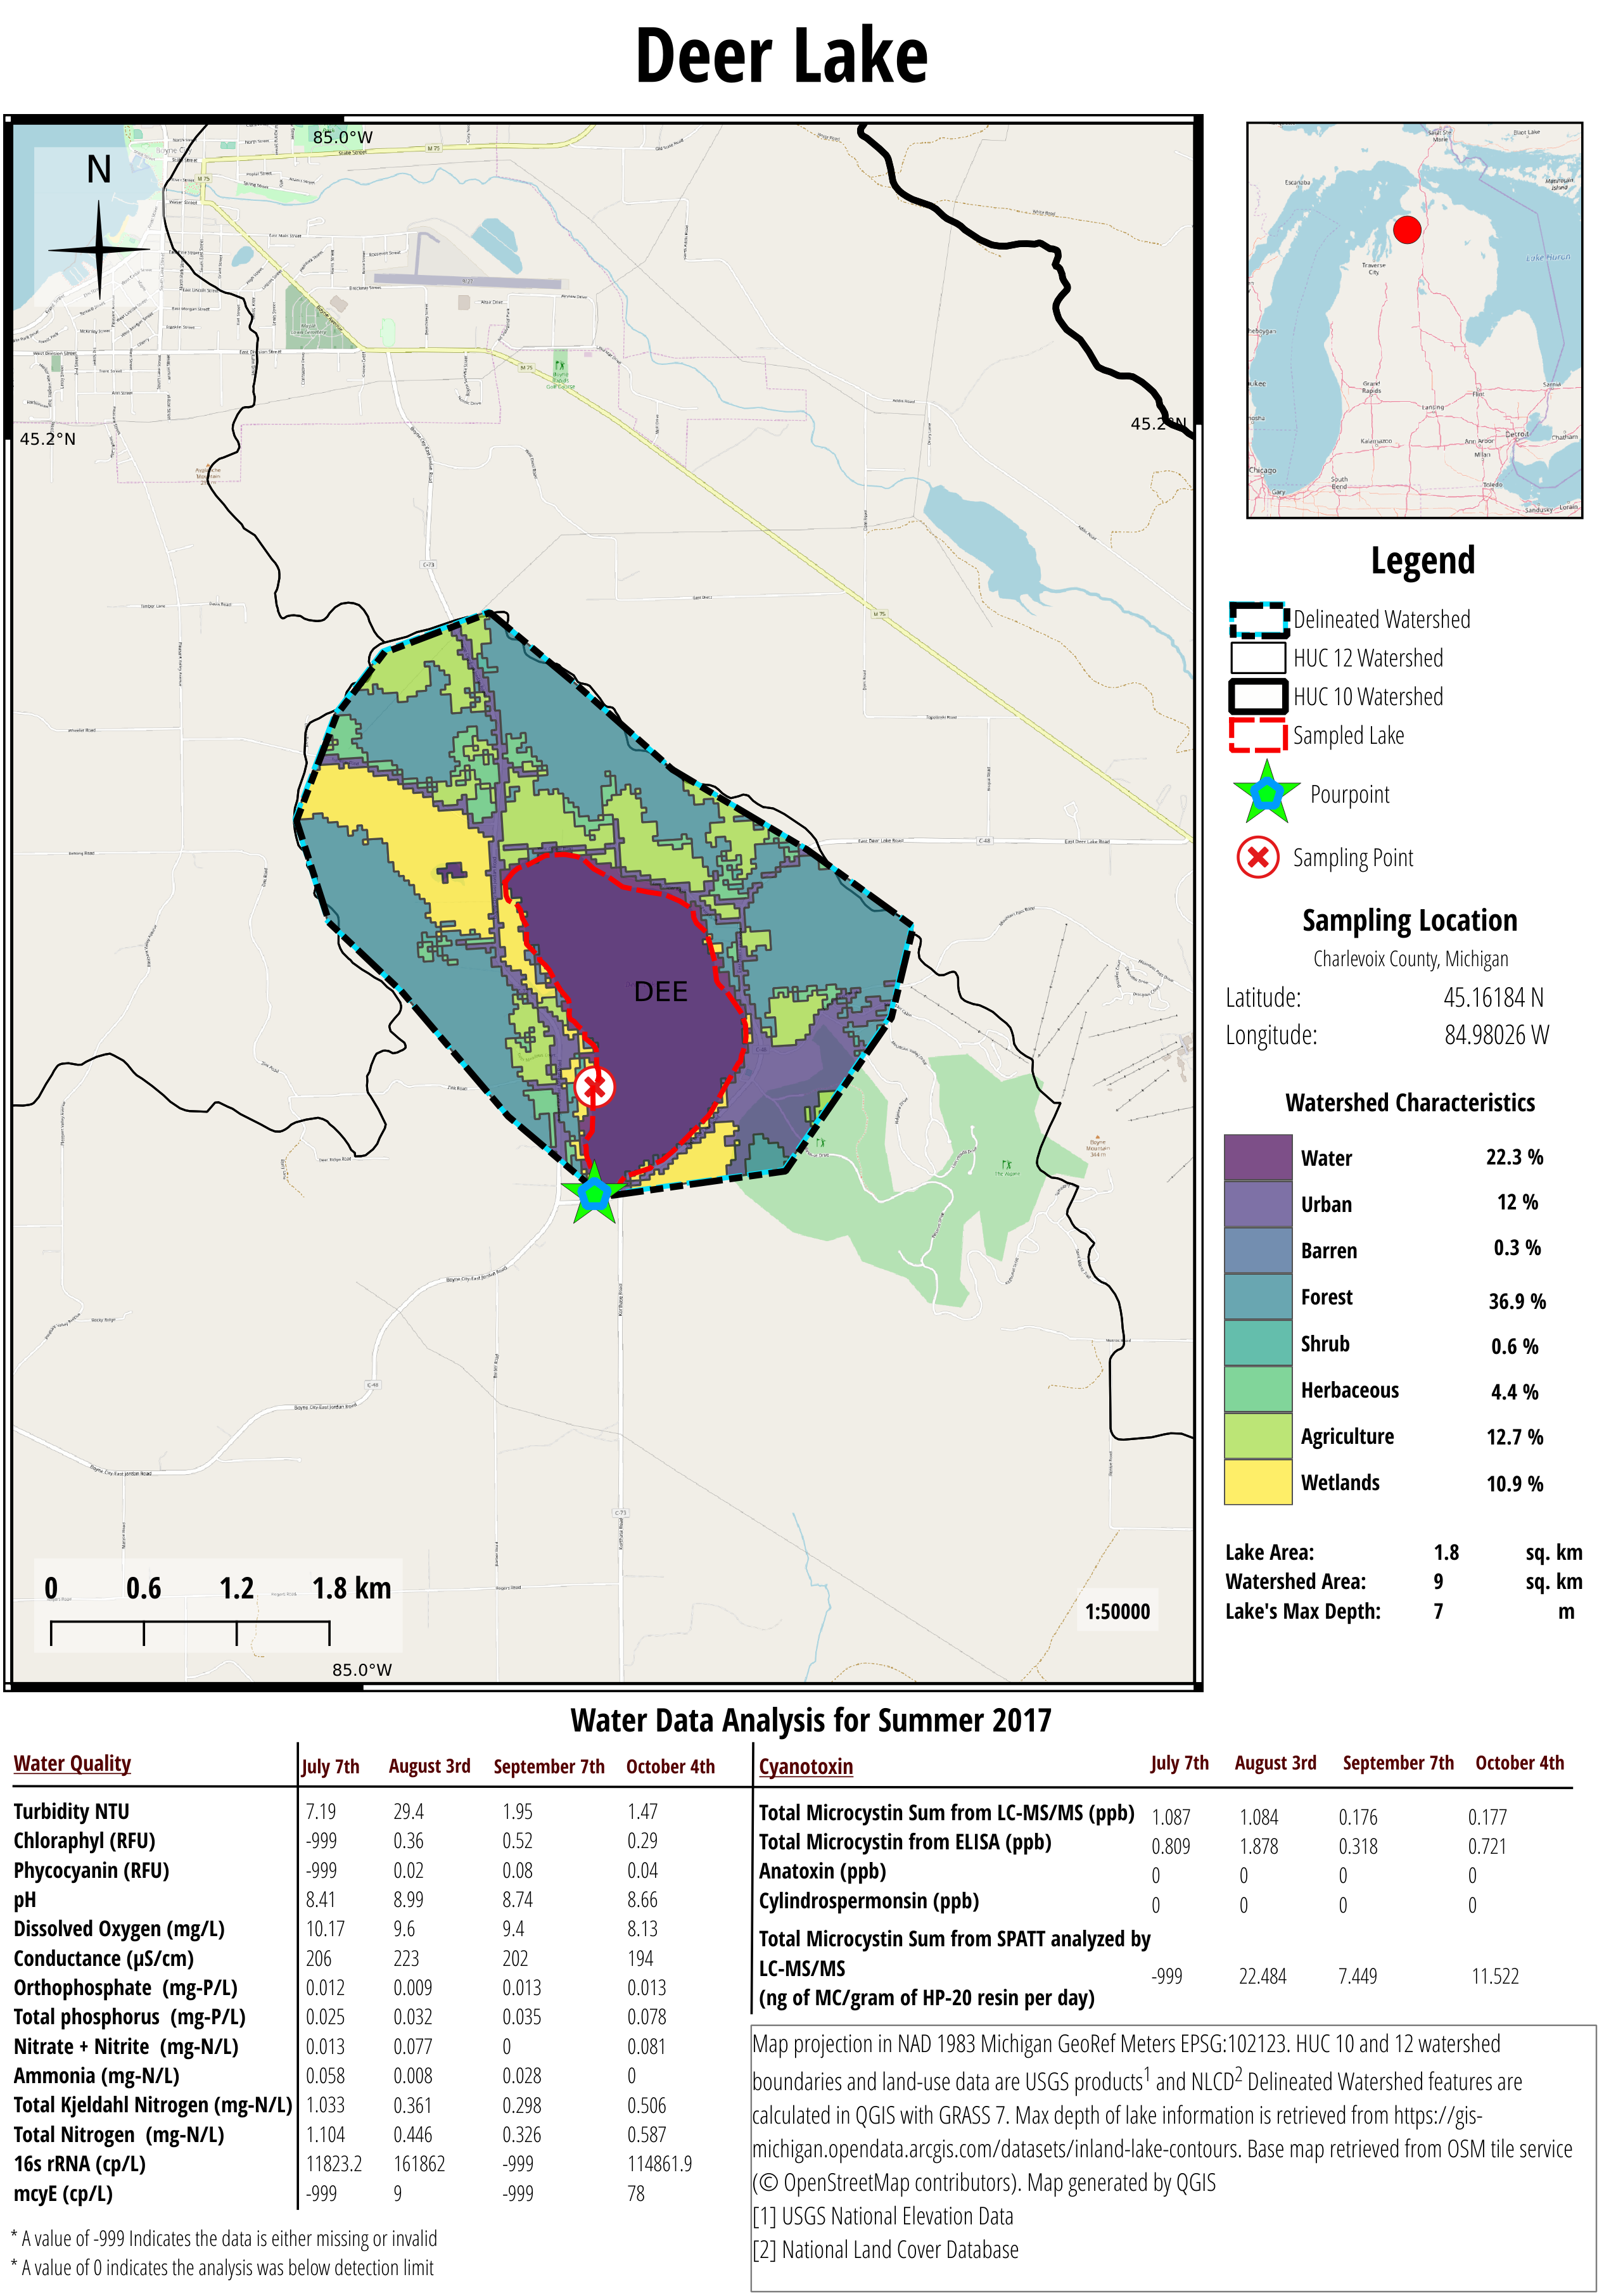
\includegraphics{figures/atlas/output_7}}
  }
\caption{GIS Map of Deer Lake}
\end{figure}

\begin{figure}[t]
\centerline{%
  \resizebox{\textwidth}{!}{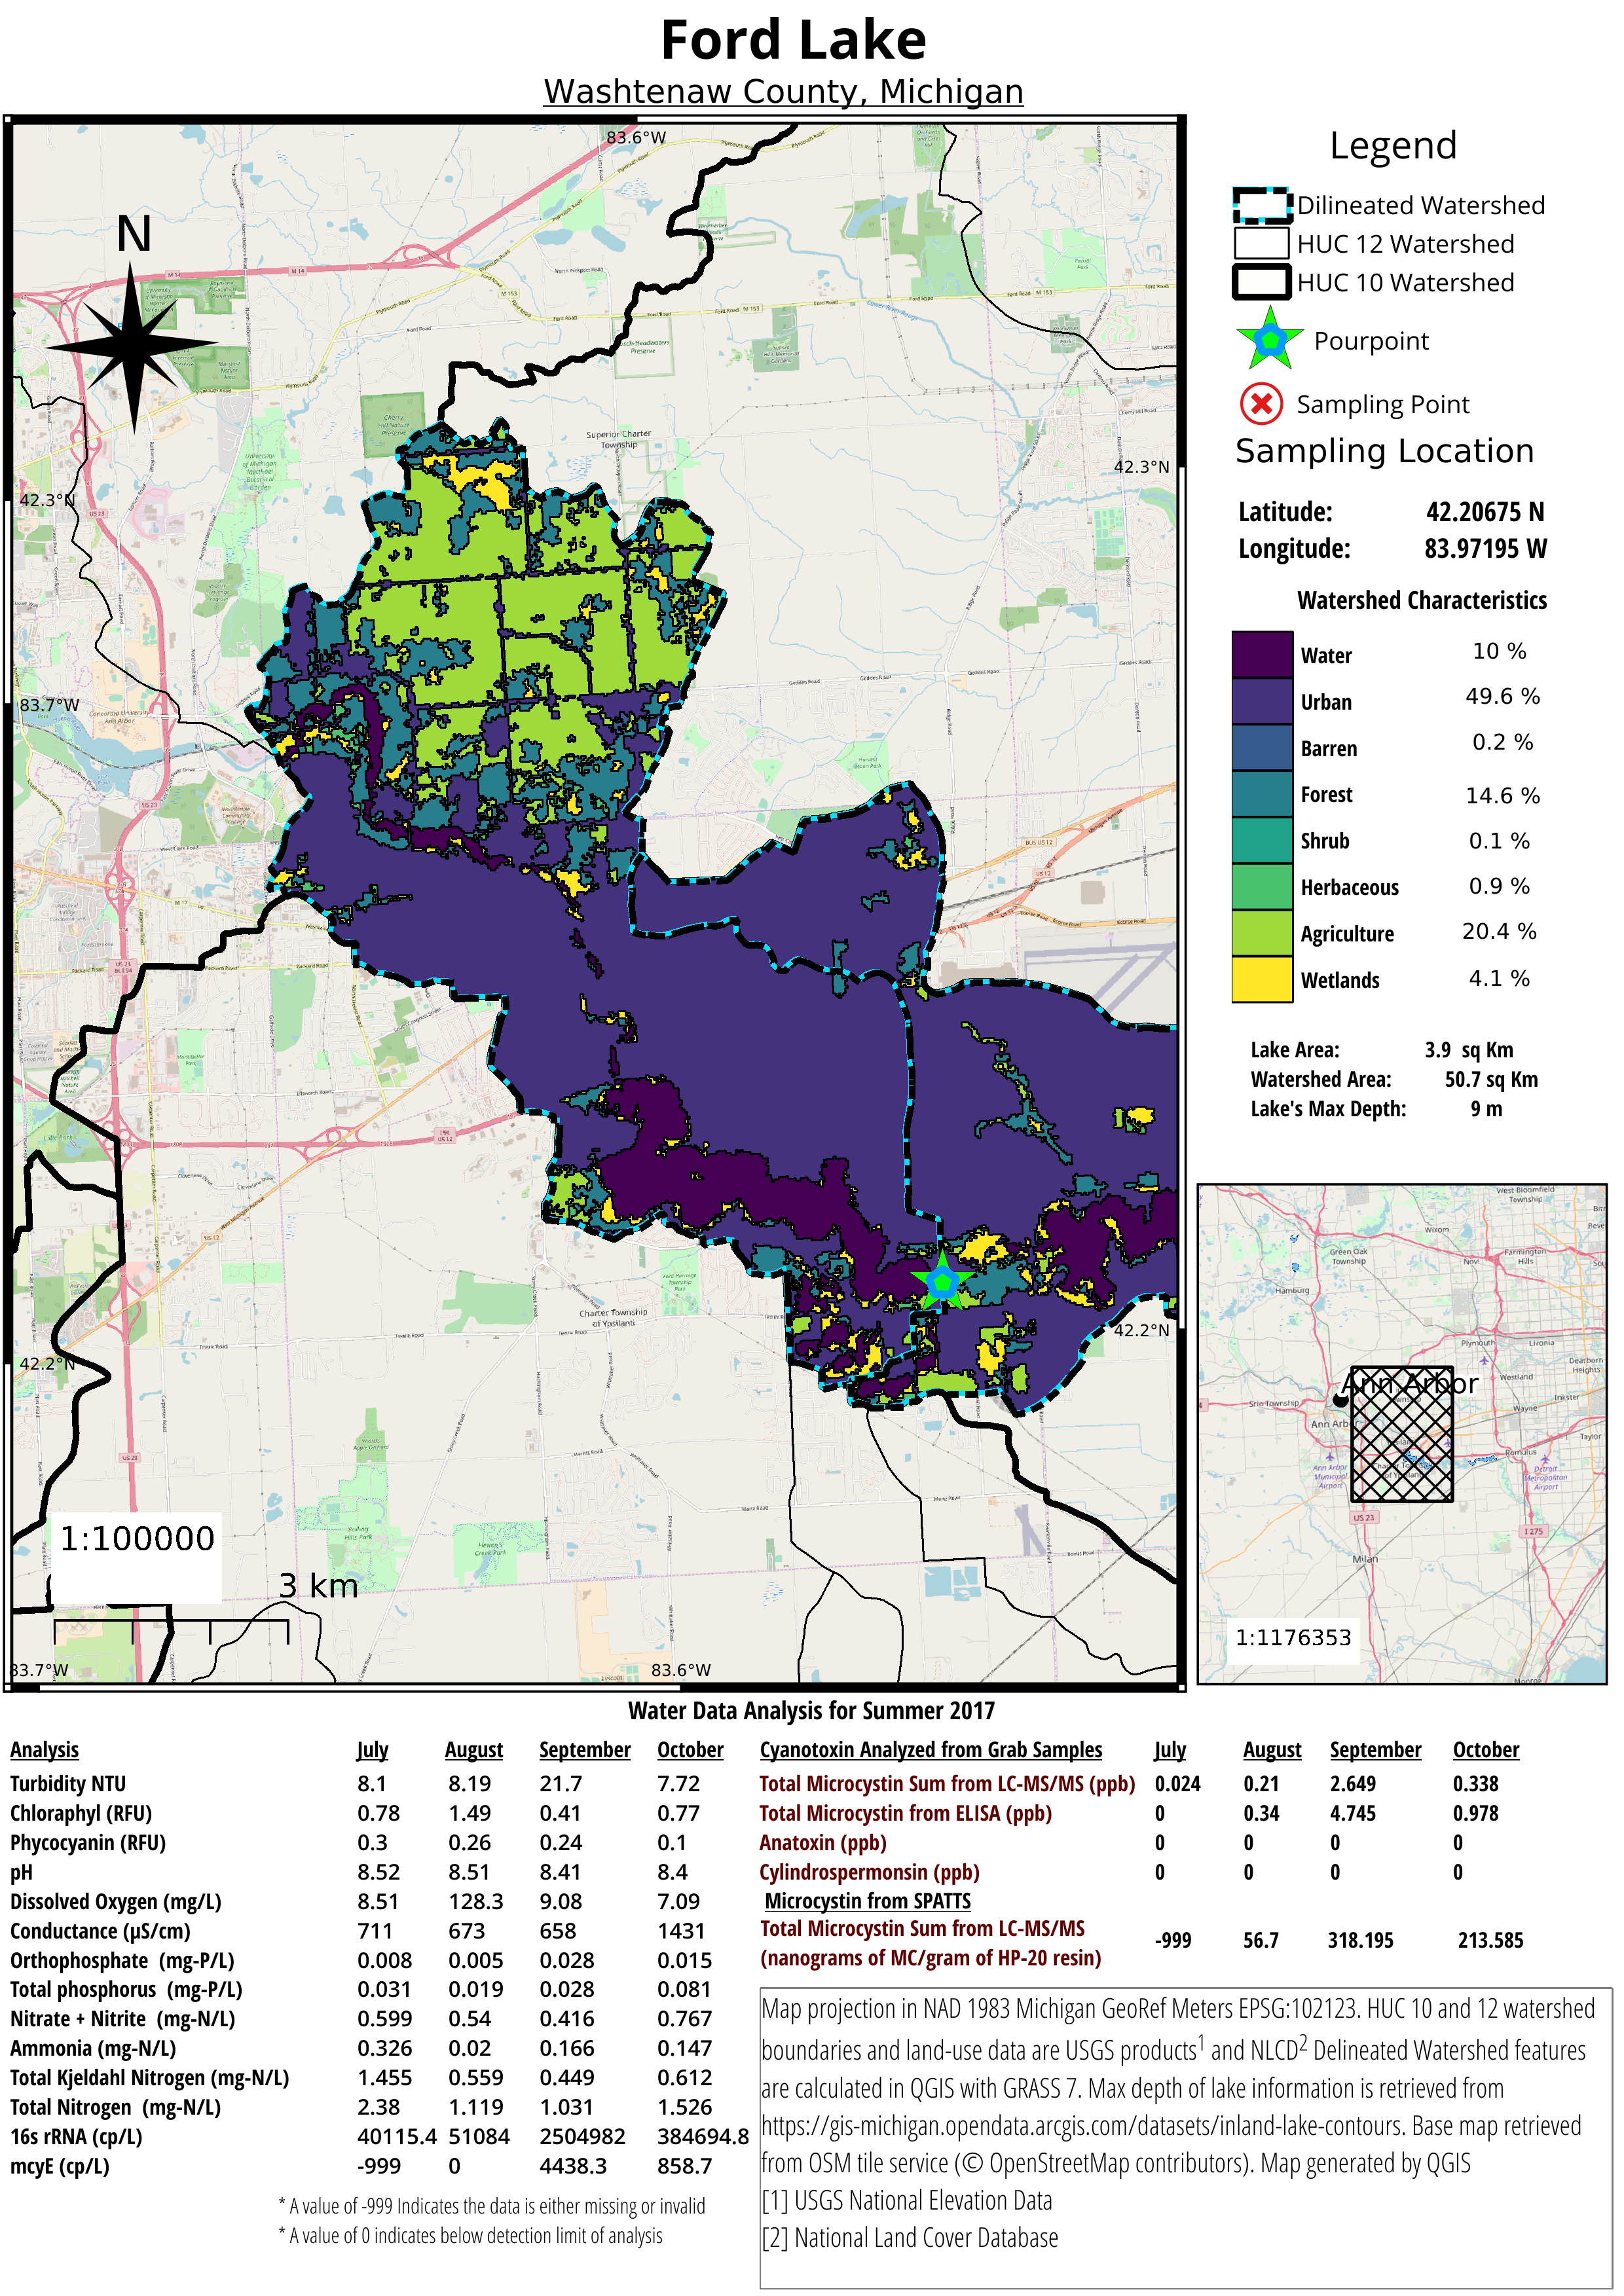
\includegraphics{figures/atlas/output_8}}
  }
\caption{GIS Map of Ford Lake}
\end{figure}

\begin{figure}[t]
\centerline{%
  \resizebox{\textwidth}{!}{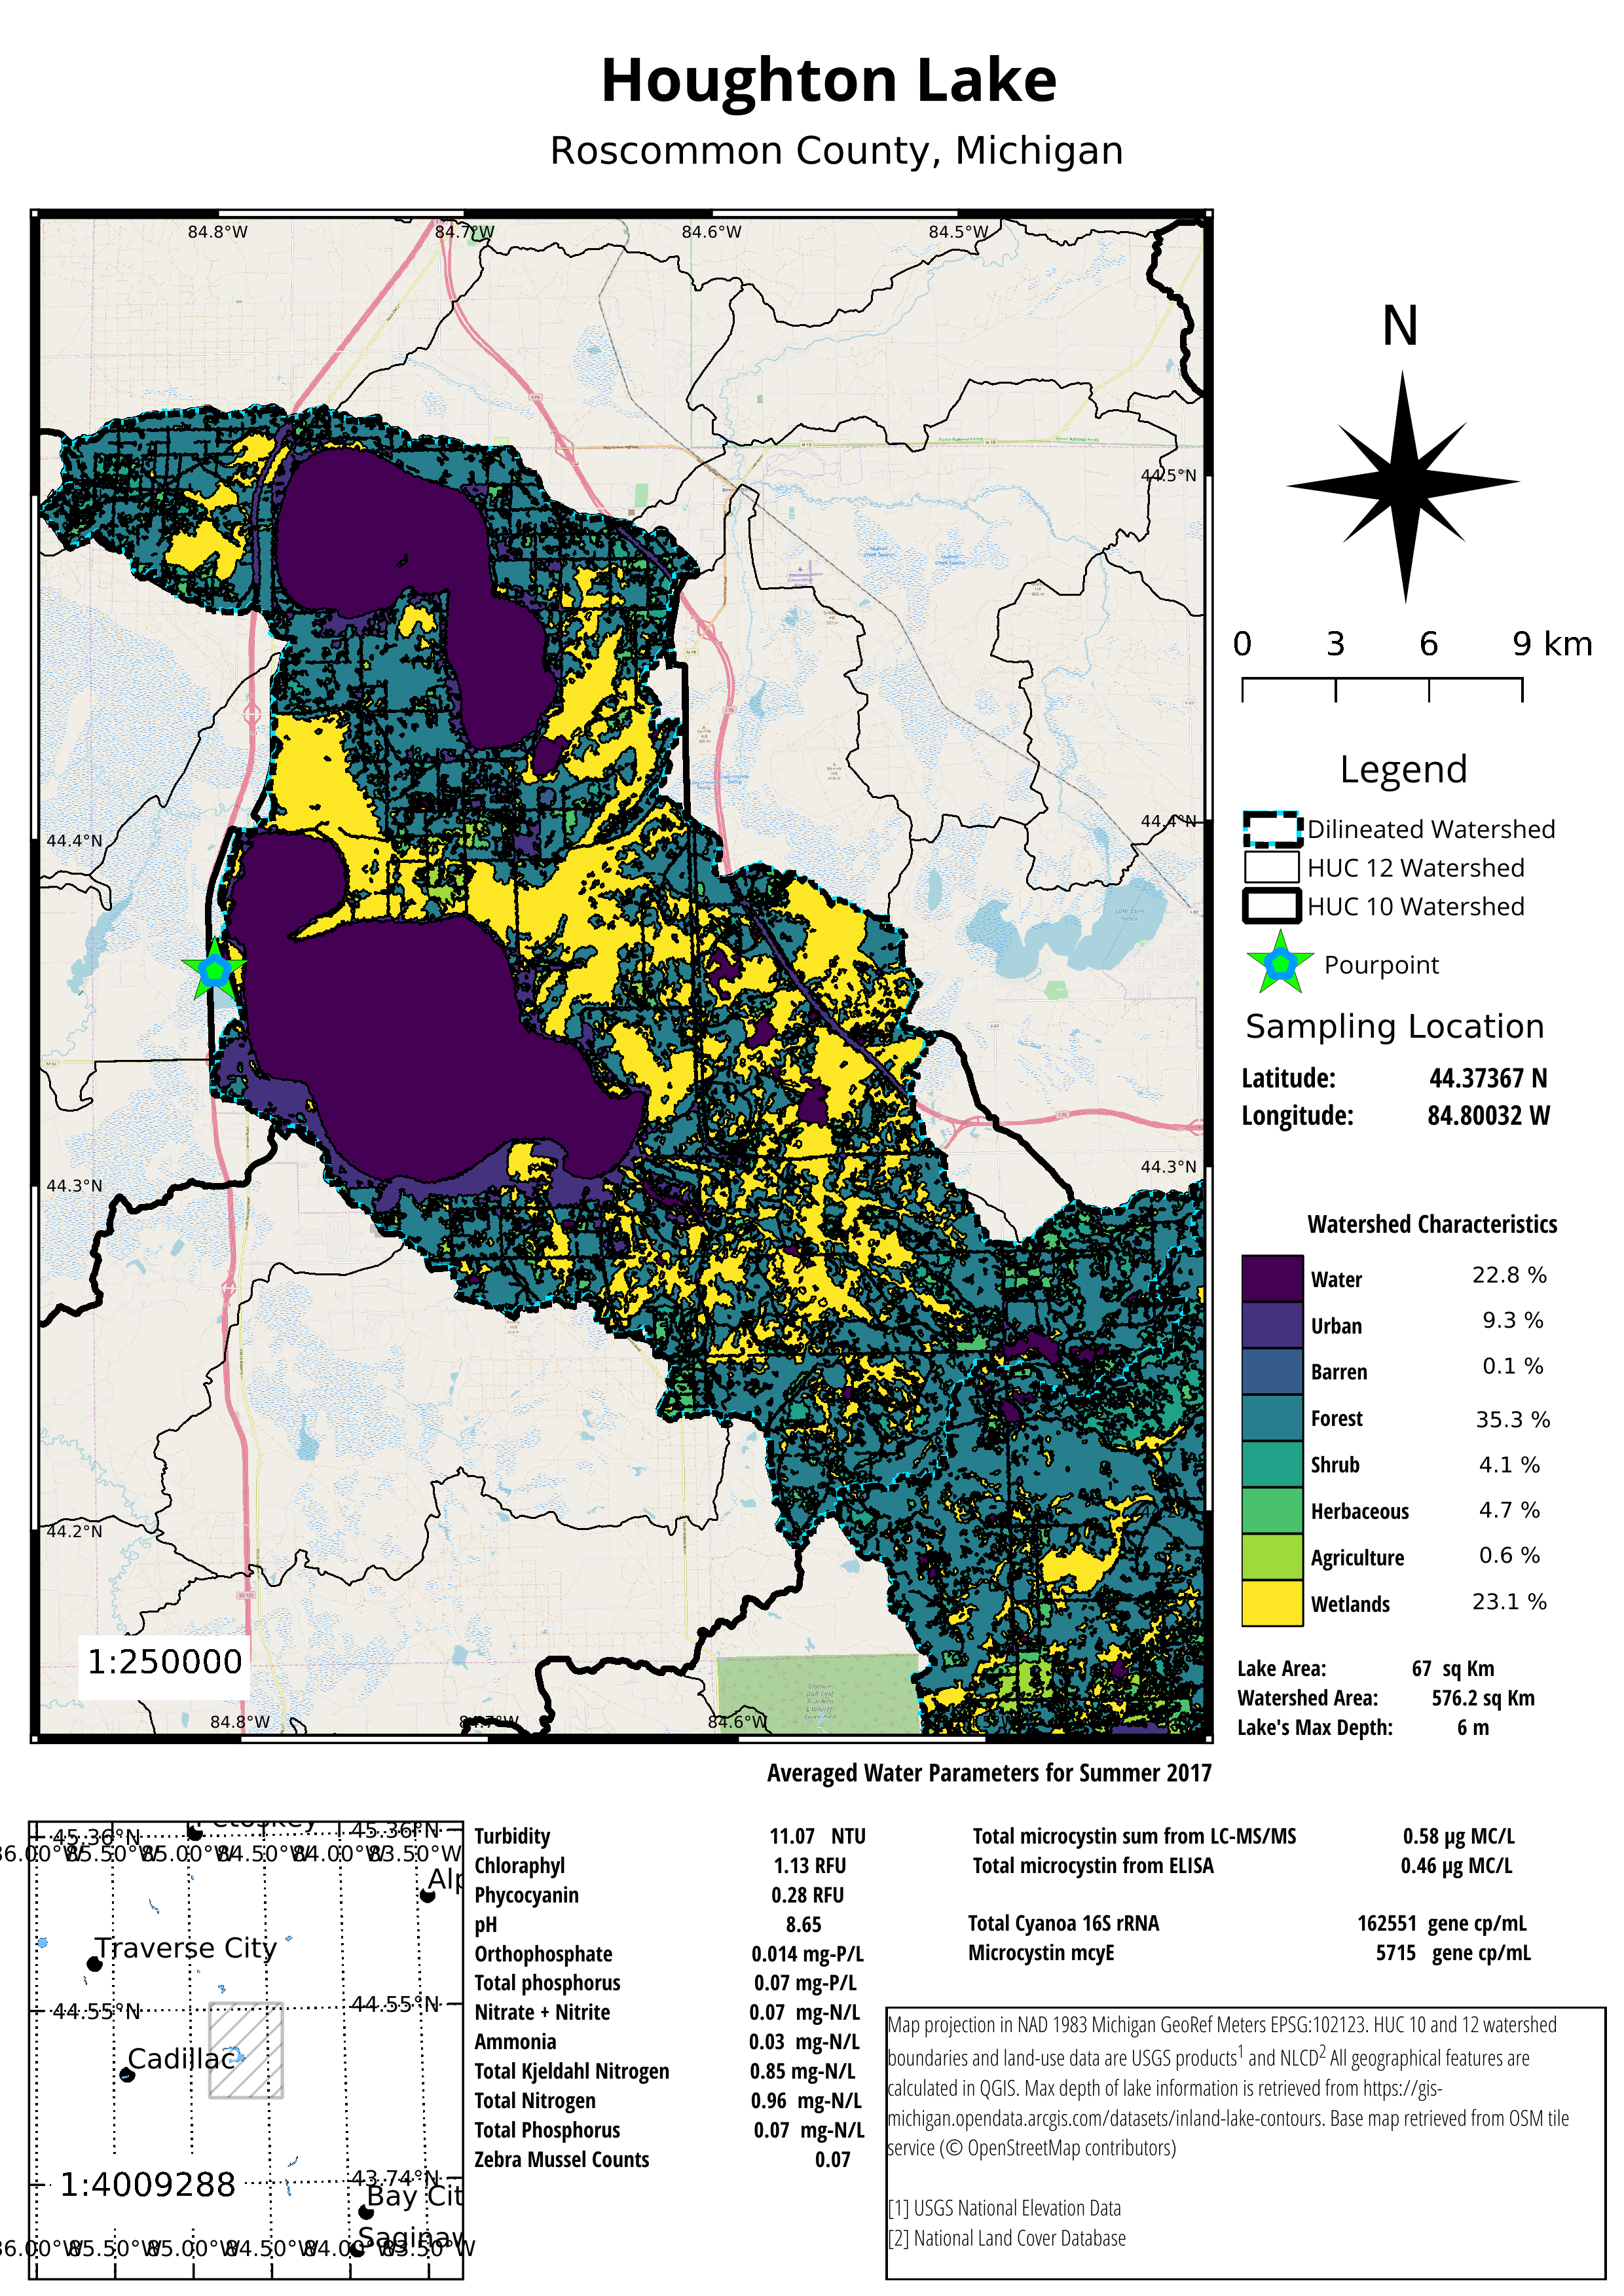
\includegraphics{figures/atlas/output_9}}
  }
\caption{GIS Map of Houghton Lake}
\end{figure}

\begin{figure}[t]
\centerline{%
  \resizebox{\textwidth}{!}{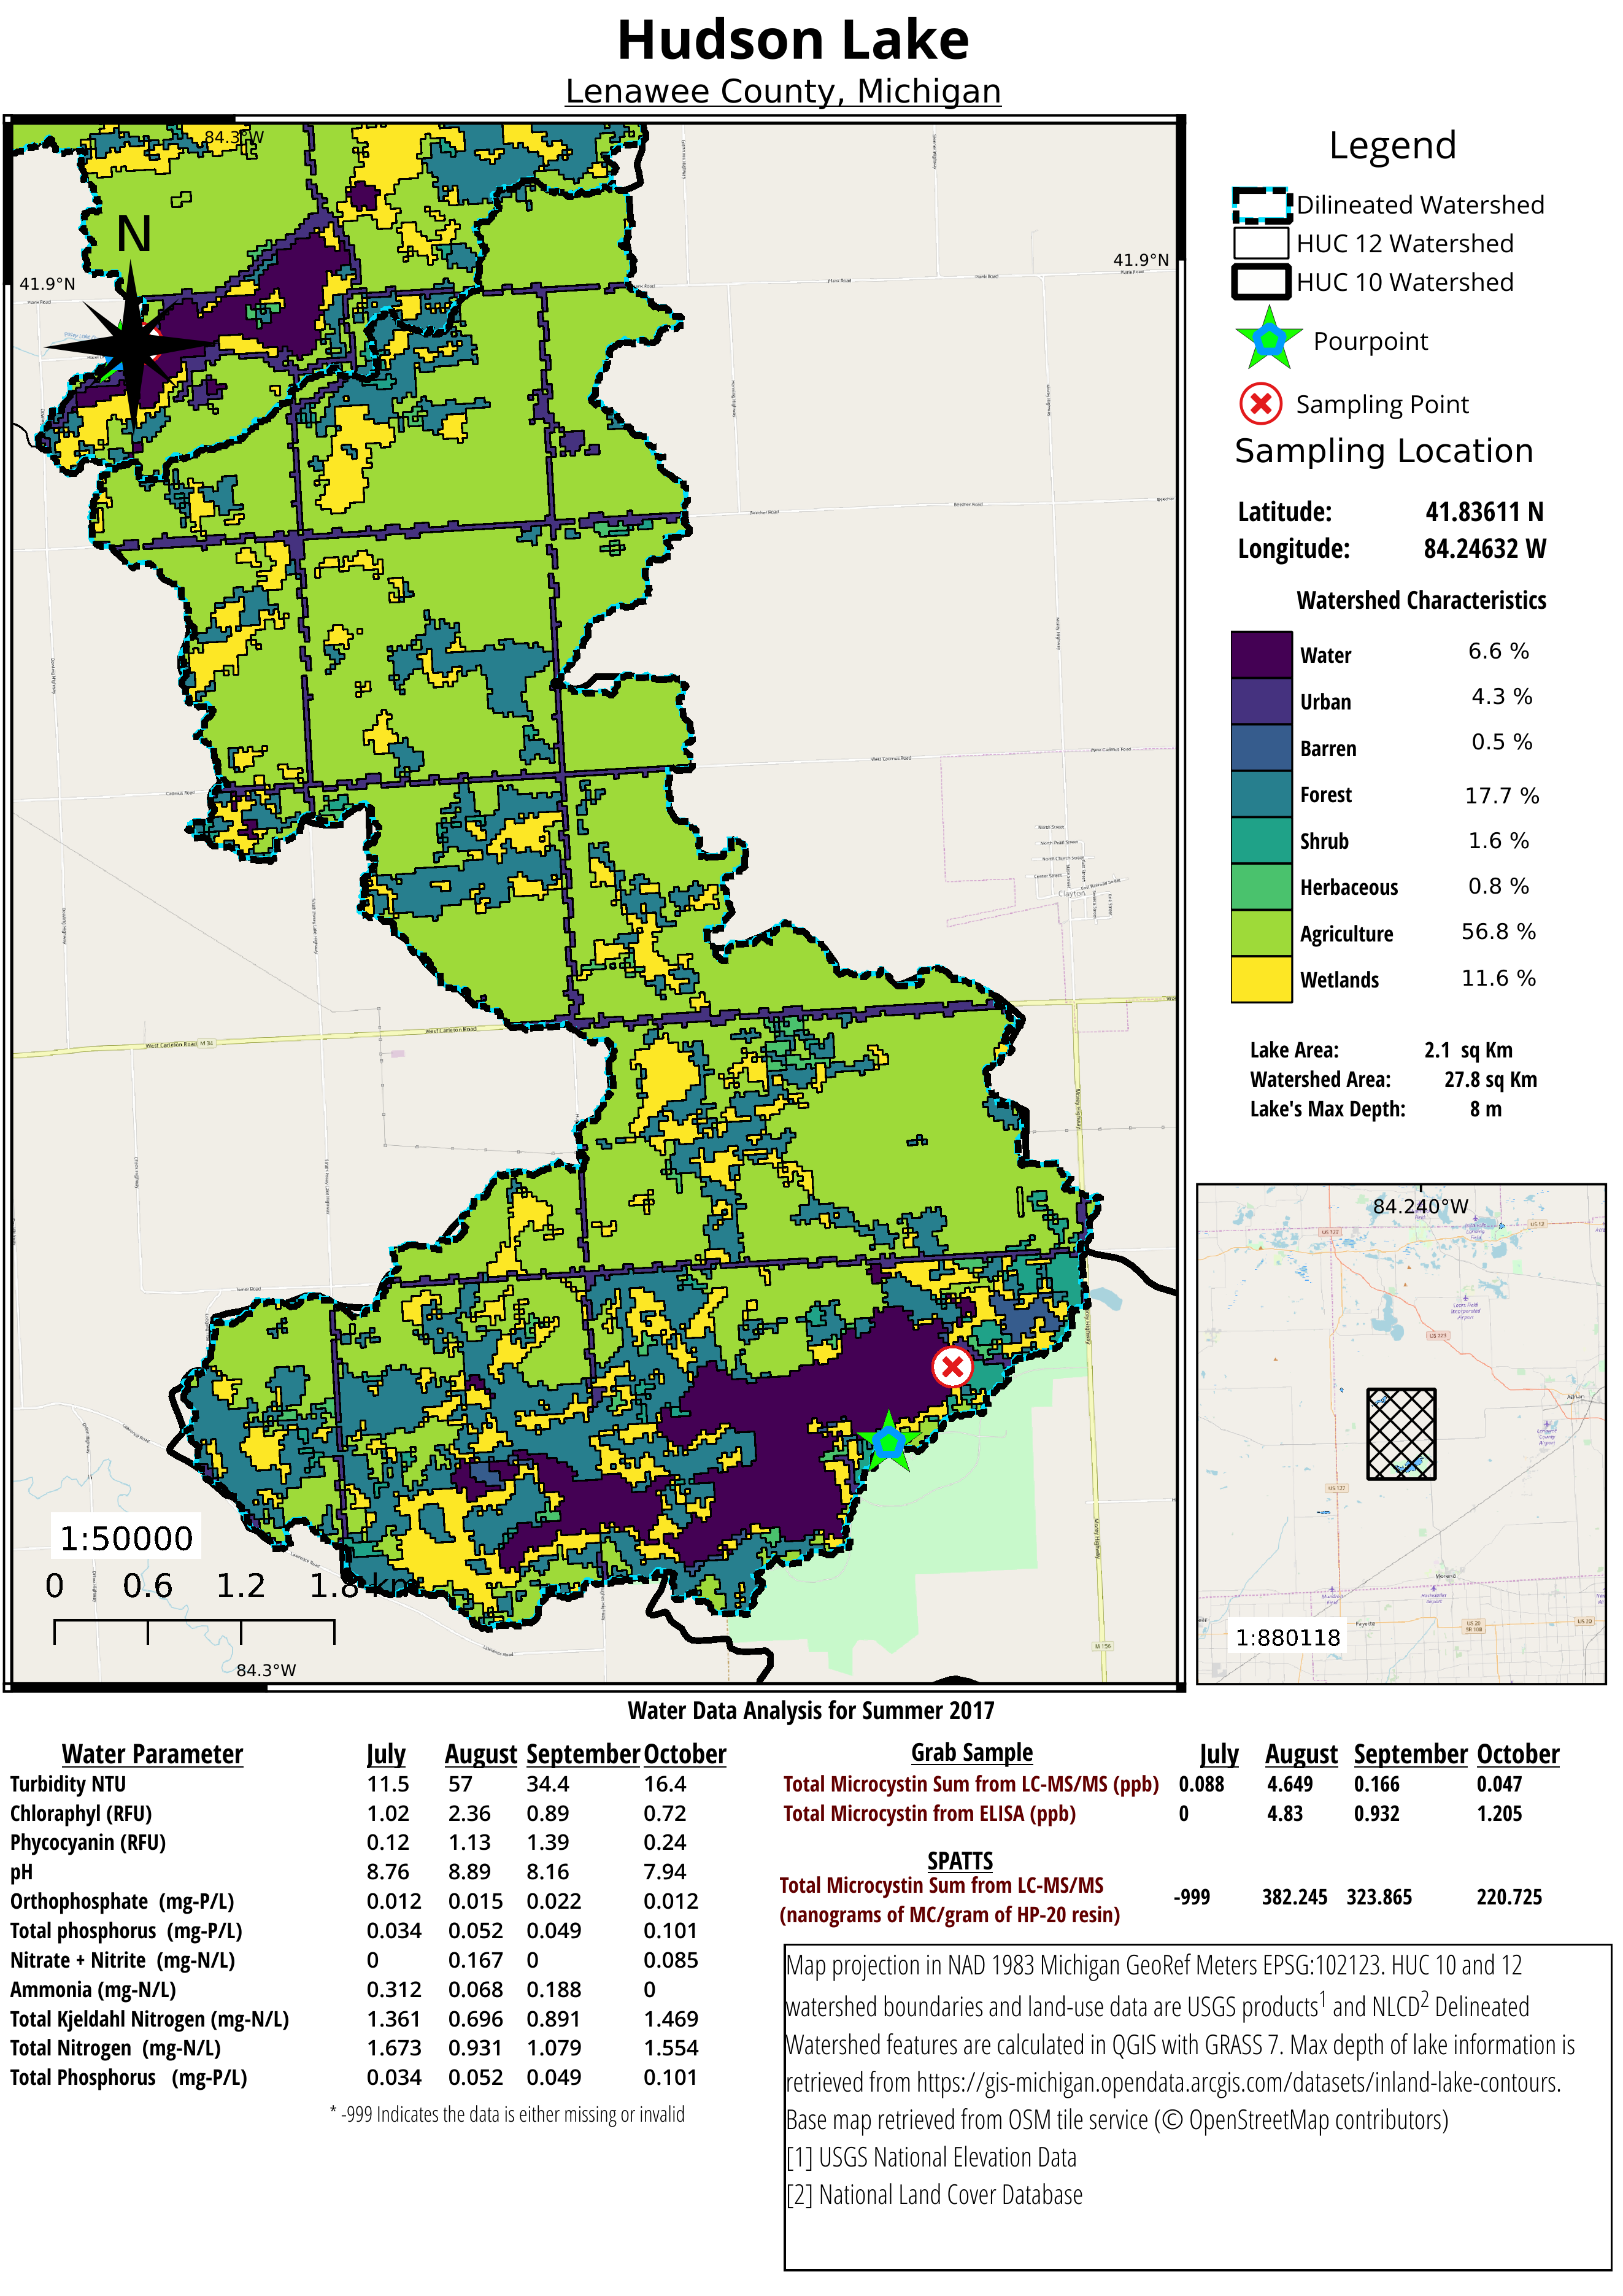
\includegraphics{figures/atlas/output_10}}
  }
\caption{GIS Map of Hudson Lake}
\end{figure}

\begin{figure}[t]
\centerline{%
  \resizebox{\textwidth}{!}{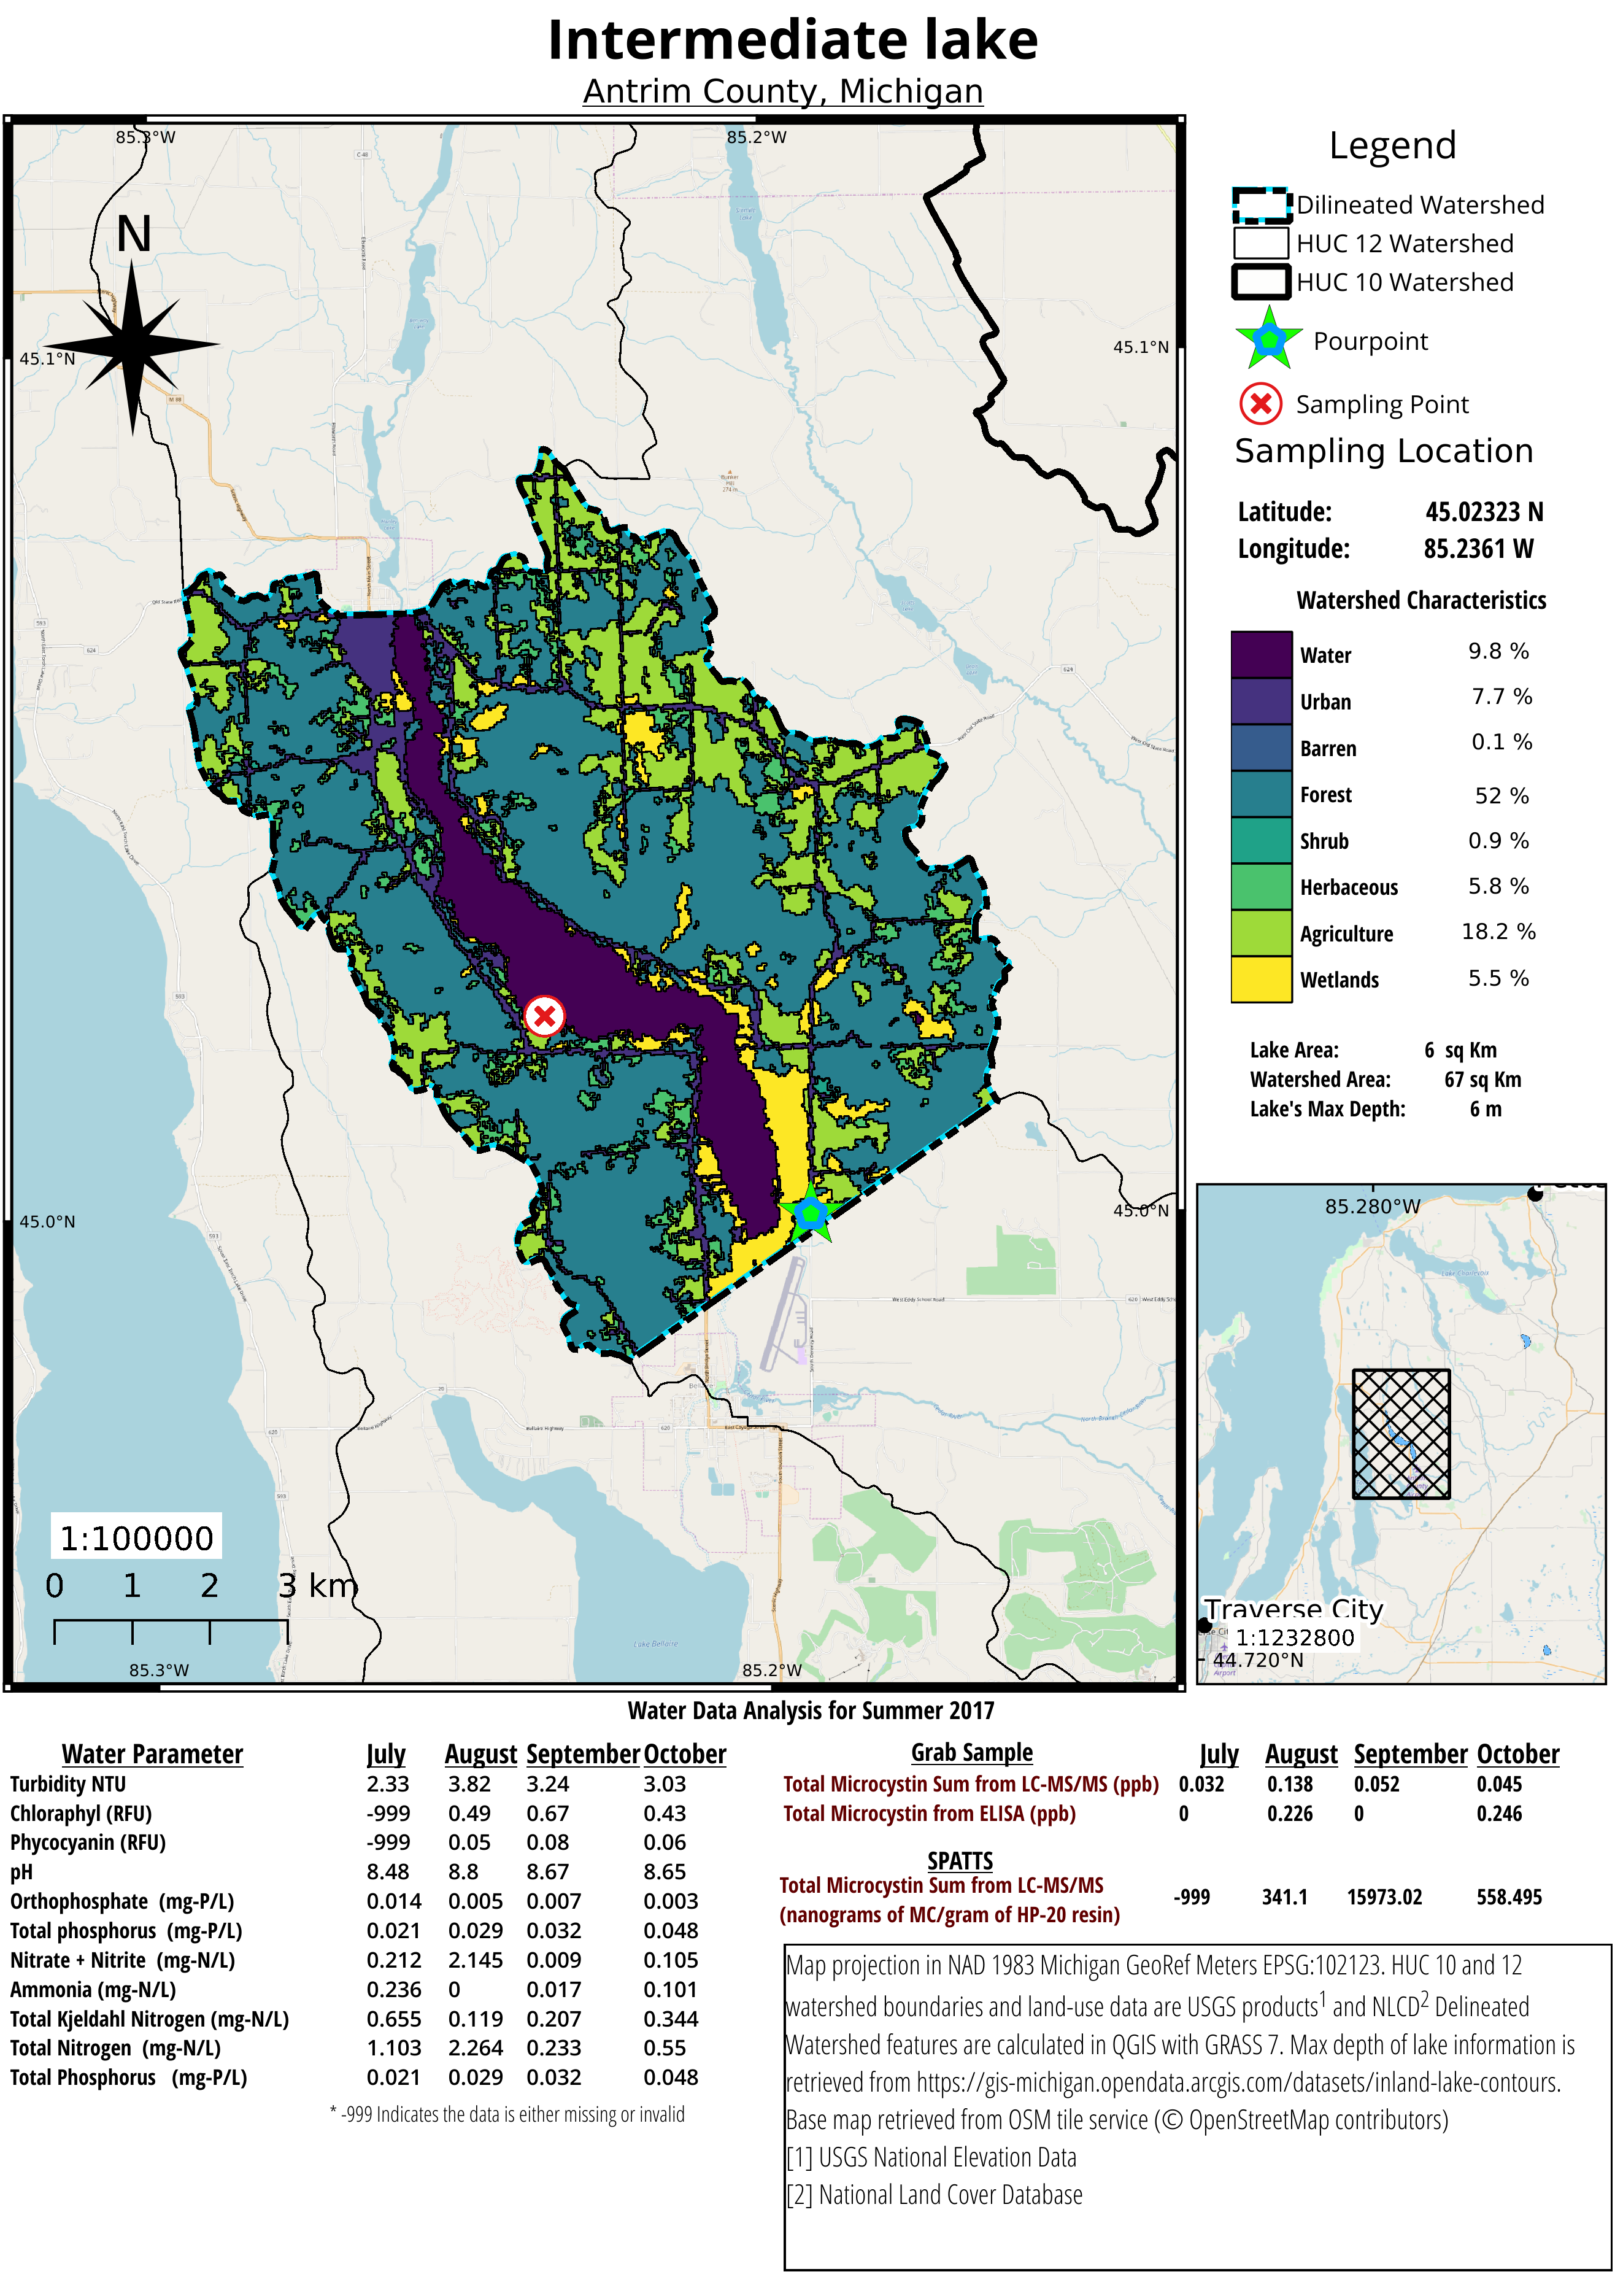
\includegraphics{figures/atlas/output_11}}
  }
\caption{GIS Map of Intermediate Lake}
\end{figure}

\begin{figure}[t]
\centerline{%
  \resizebox{\textwidth}{!}{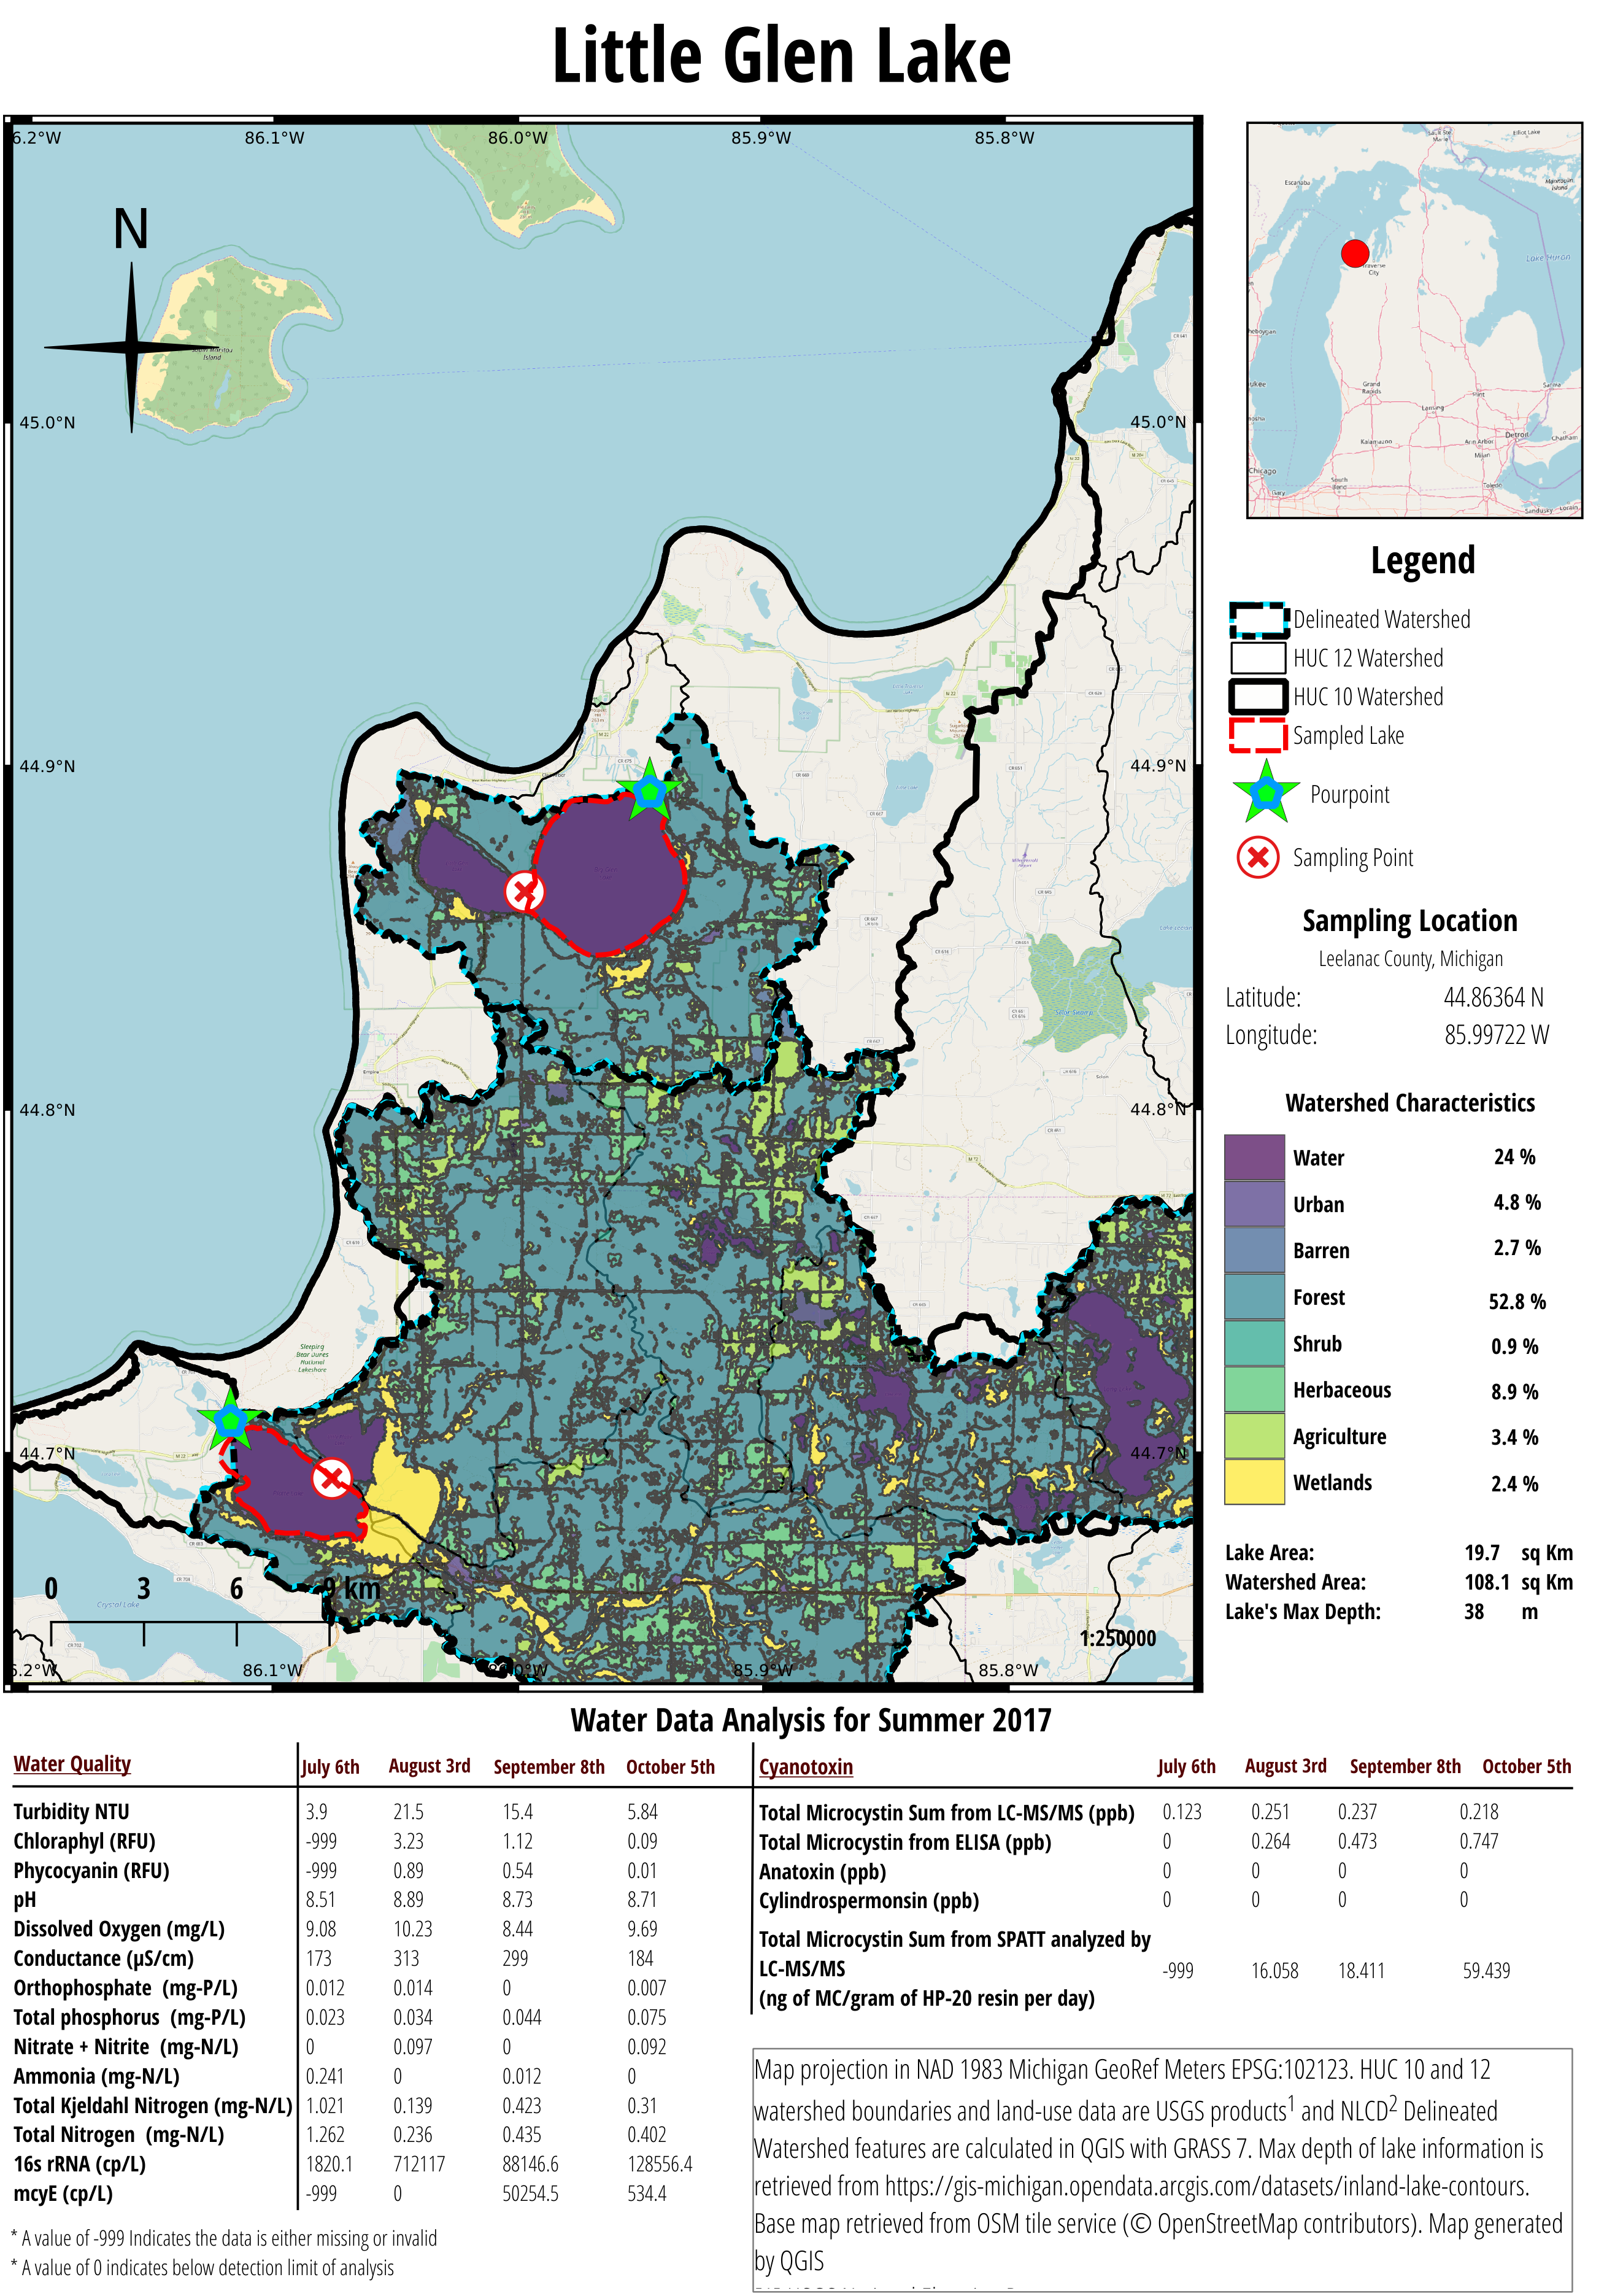
\includegraphics{figures/atlas/output_12}}
  }
\caption{GIS Map of Little Glen Lake}
\end{figure}

\begin{figure}[t]
\centerline{%
  \resizebox{\textwidth}{!}{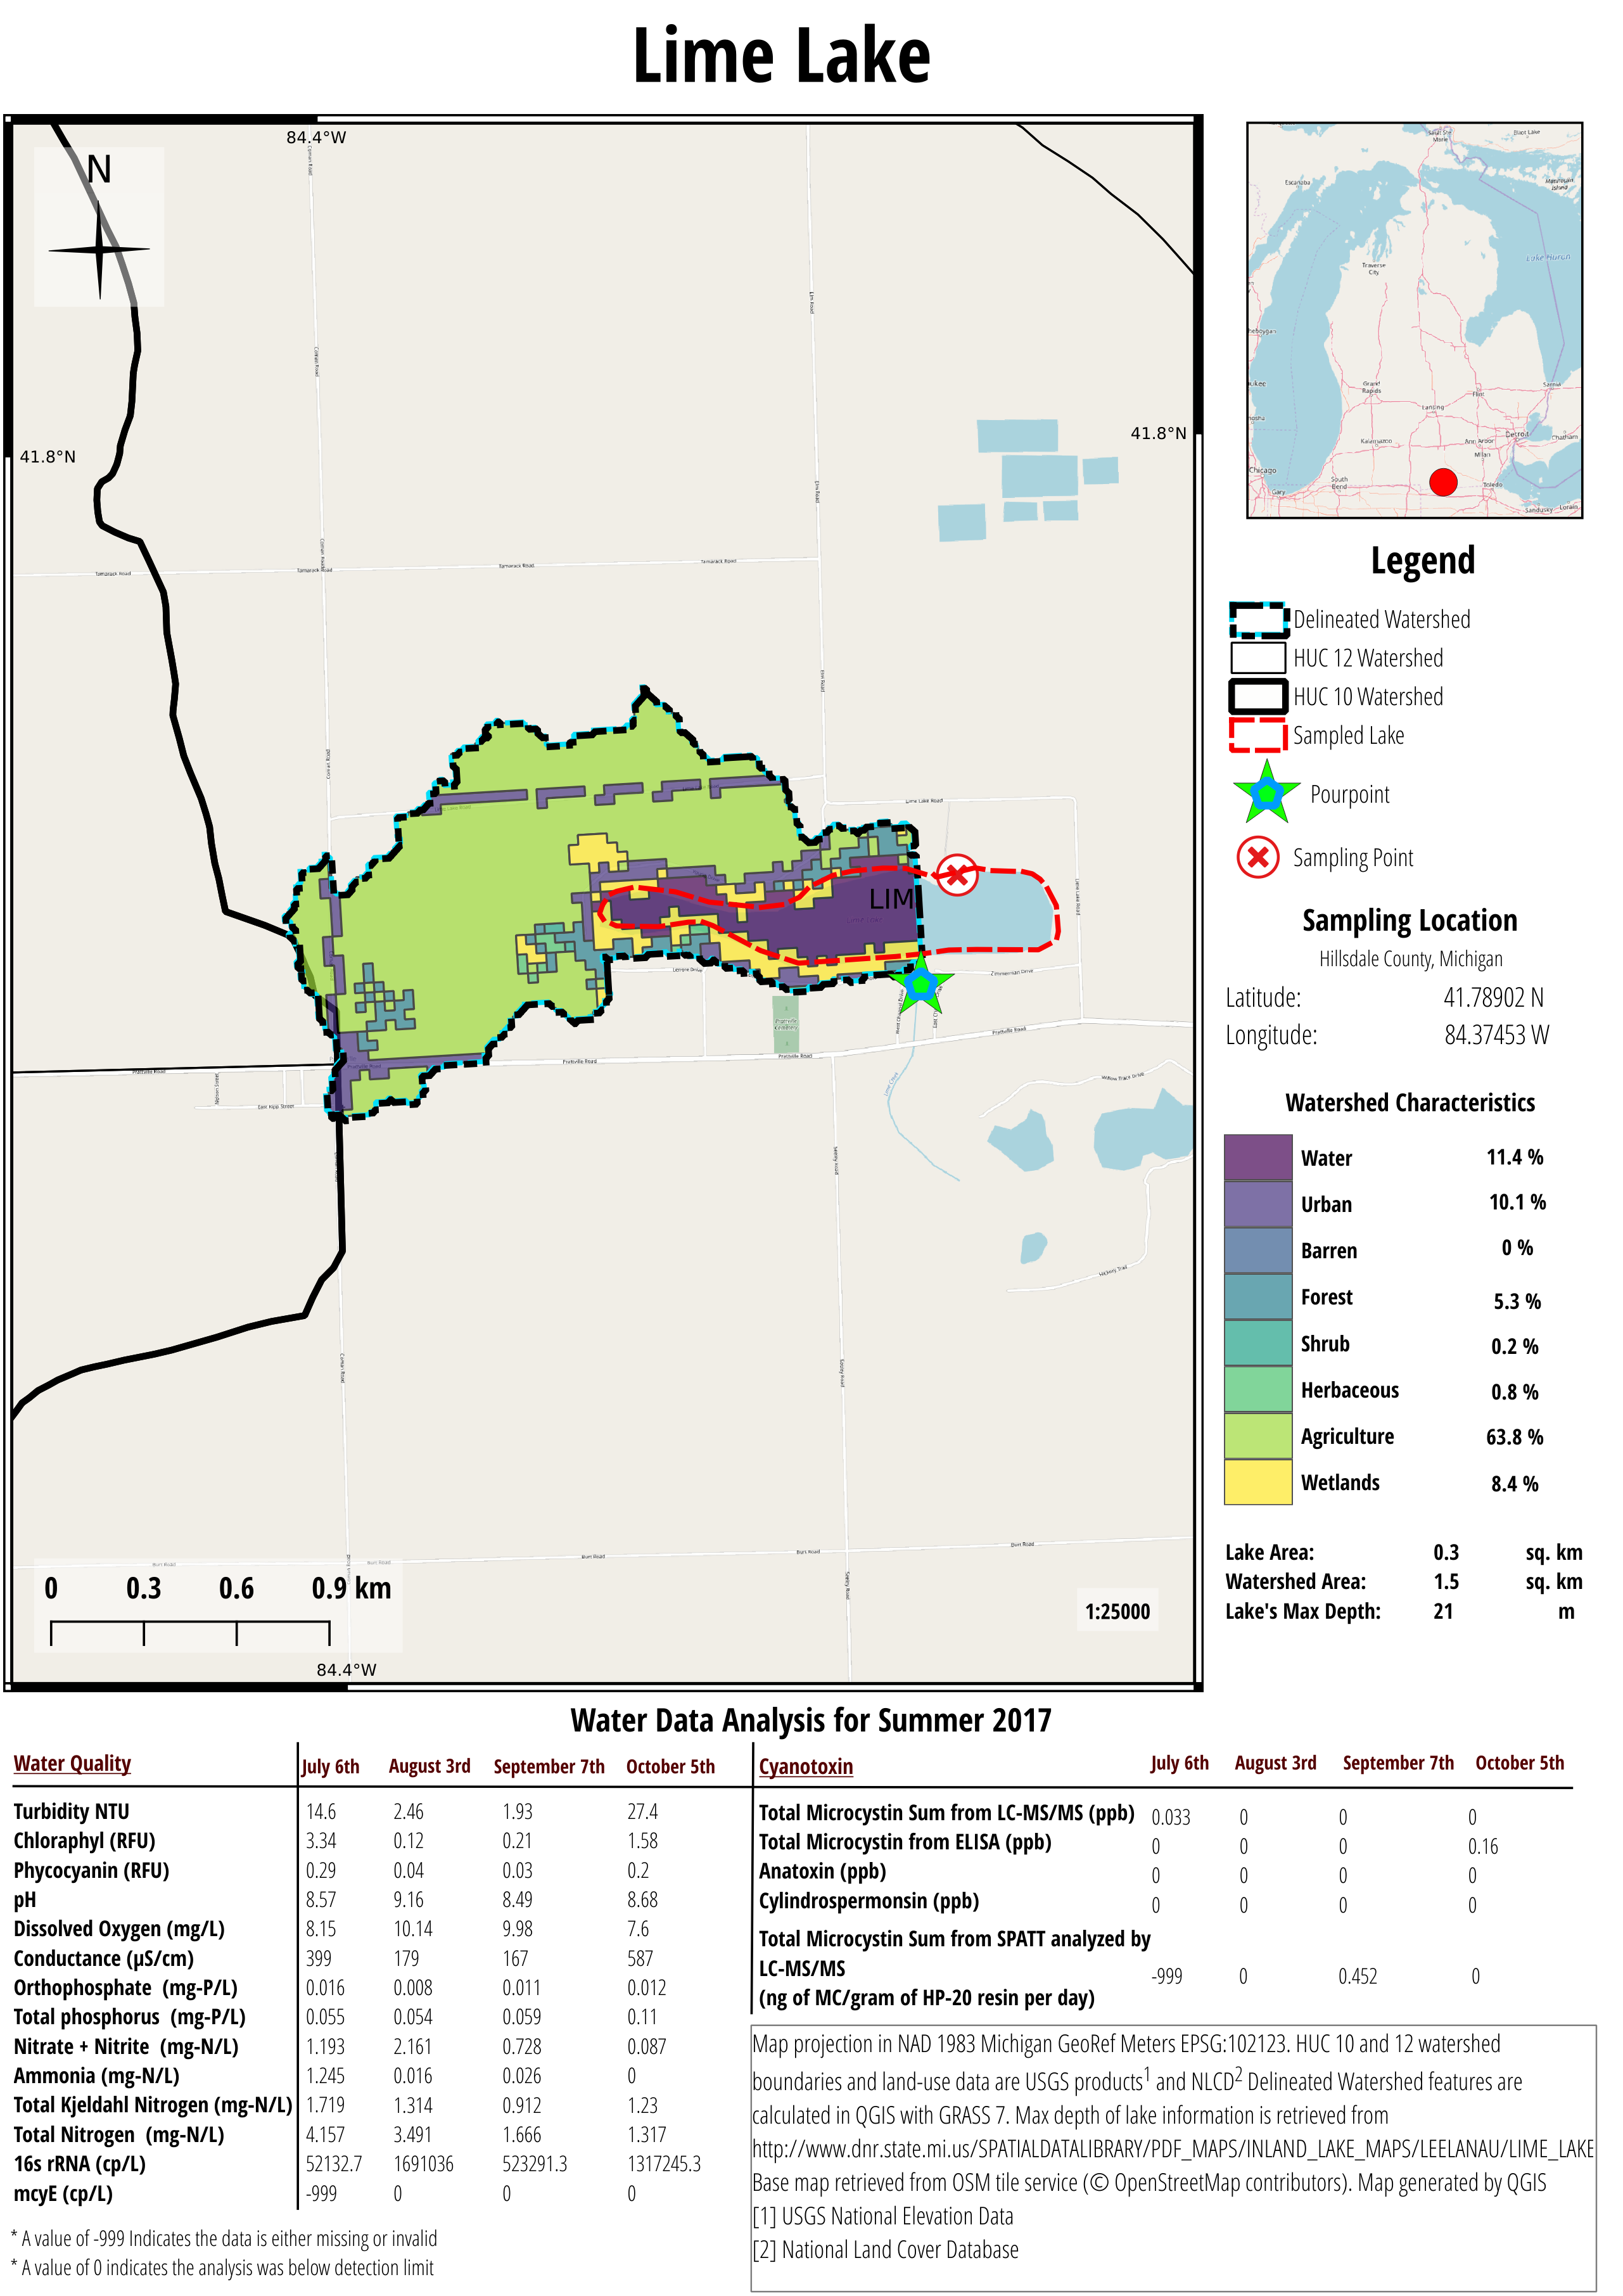
\includegraphics{figures/atlas/output_13}}
  }
\caption{GIS Map of Lime Lake}
\end{figure}

\begin{figure}[t]
\centerline{%
  \resizebox{\textwidth}{!}{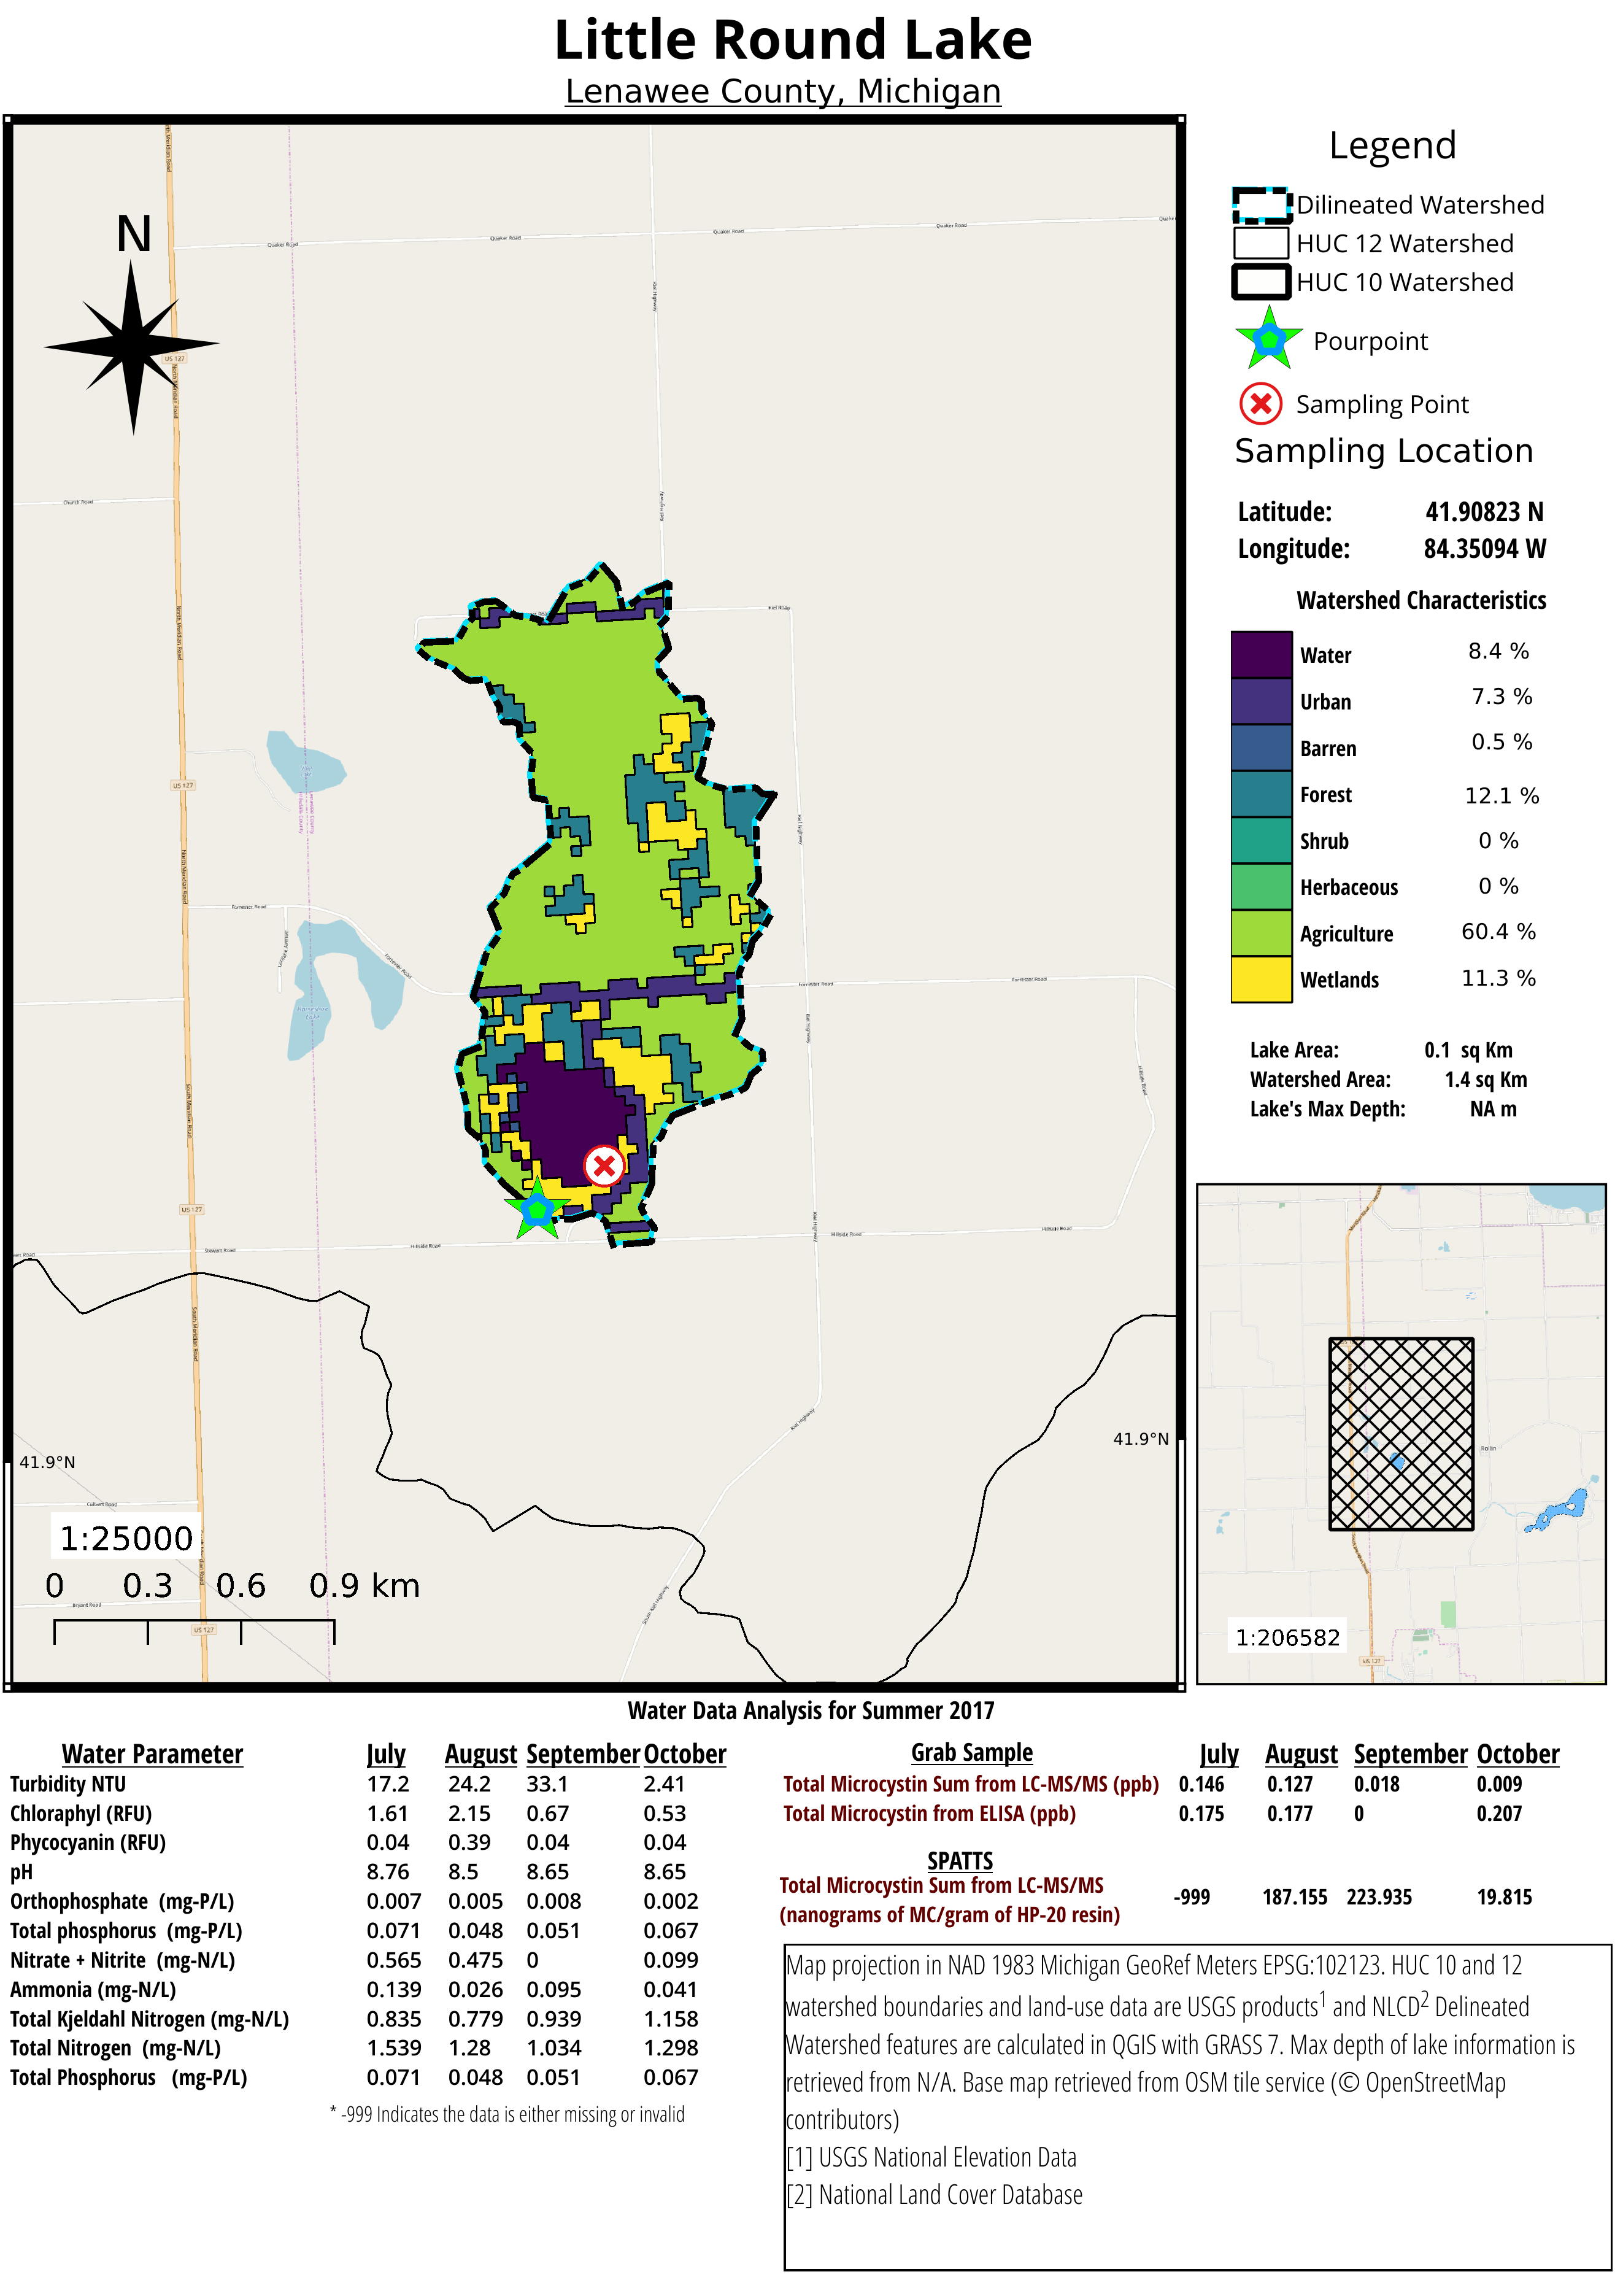
\includegraphics{figures/atlas/output_14}}
  }
\caption{GIS Map of Little Round Lake}
\end{figure}

\begin{figure}[t]
\centerline{%
  \resizebox{\textwidth}{!}{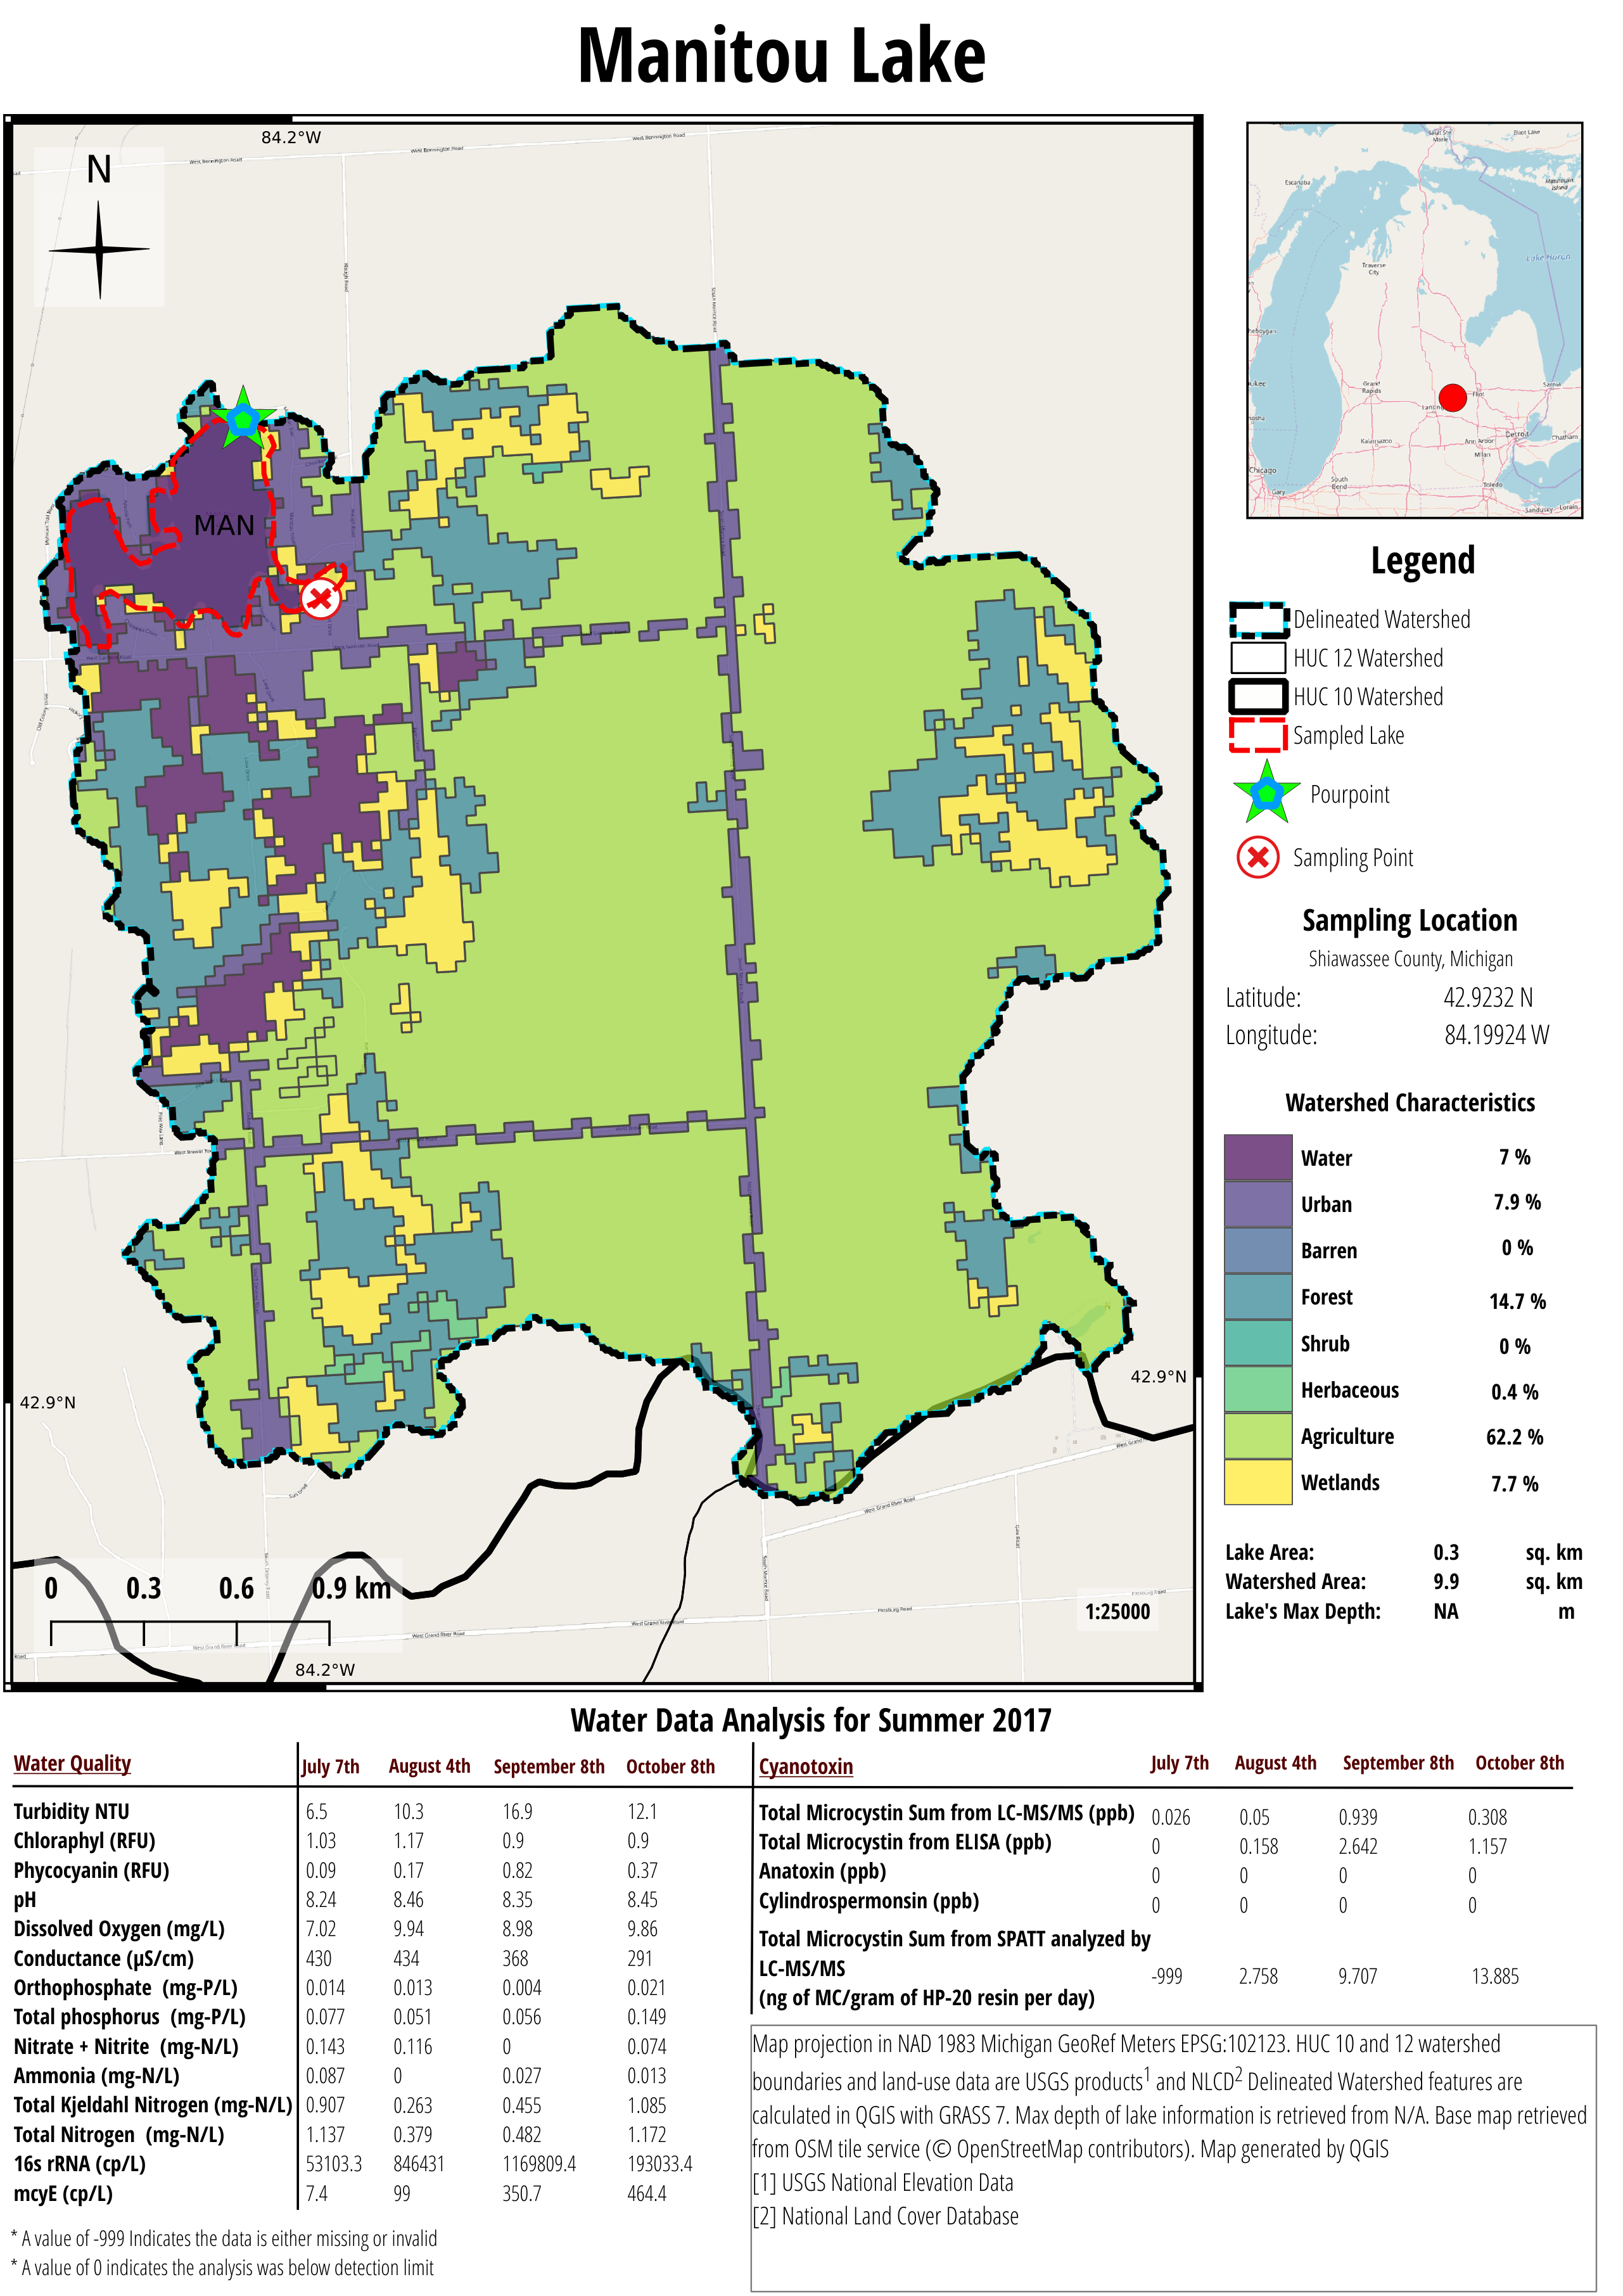
\includegraphics{figures/atlas/output_15}}
  }
\caption{GIS Map of Manitou Lake}
\end{figure}

\begin{figure}[t]
\centerline{%
  \resizebox{\textwidth}{!}{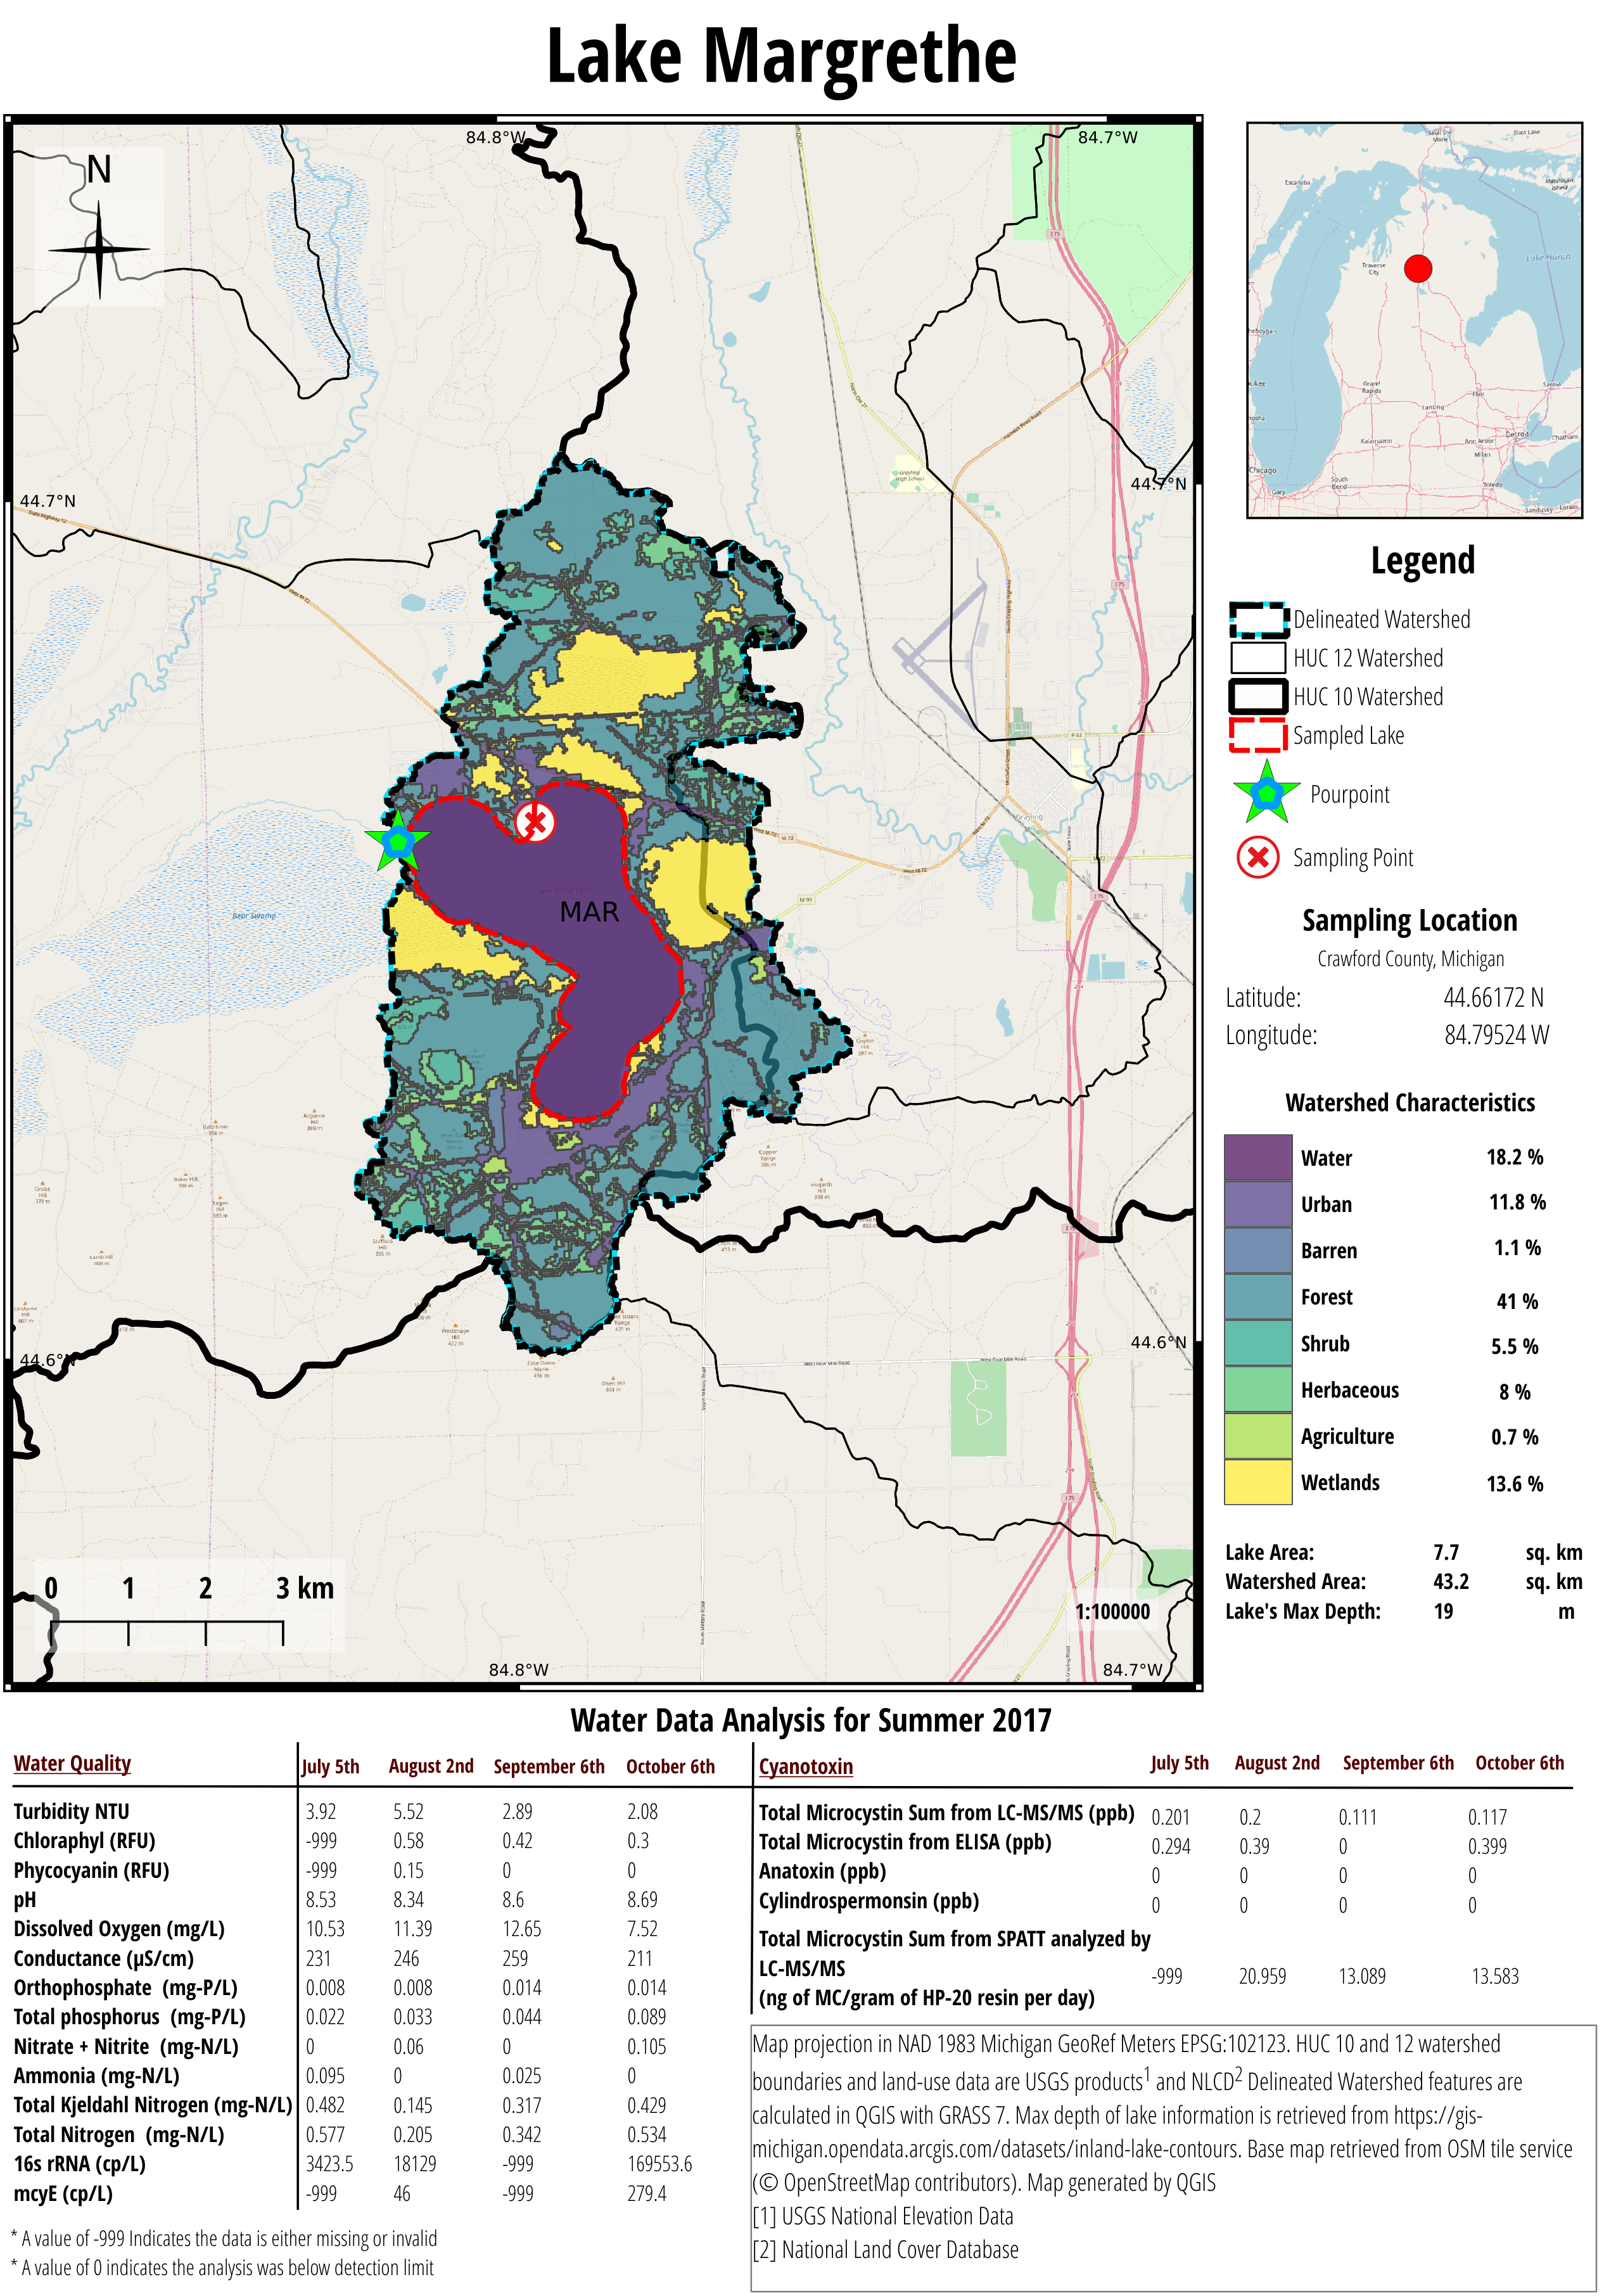
\includegraphics{figures/atlas/output_16}}
  }
\caption{GIS Map of Lake Margrethe}
\end{figure}

\begin{figure}[t]
\centerline{%
  \resizebox{\textwidth}{!}{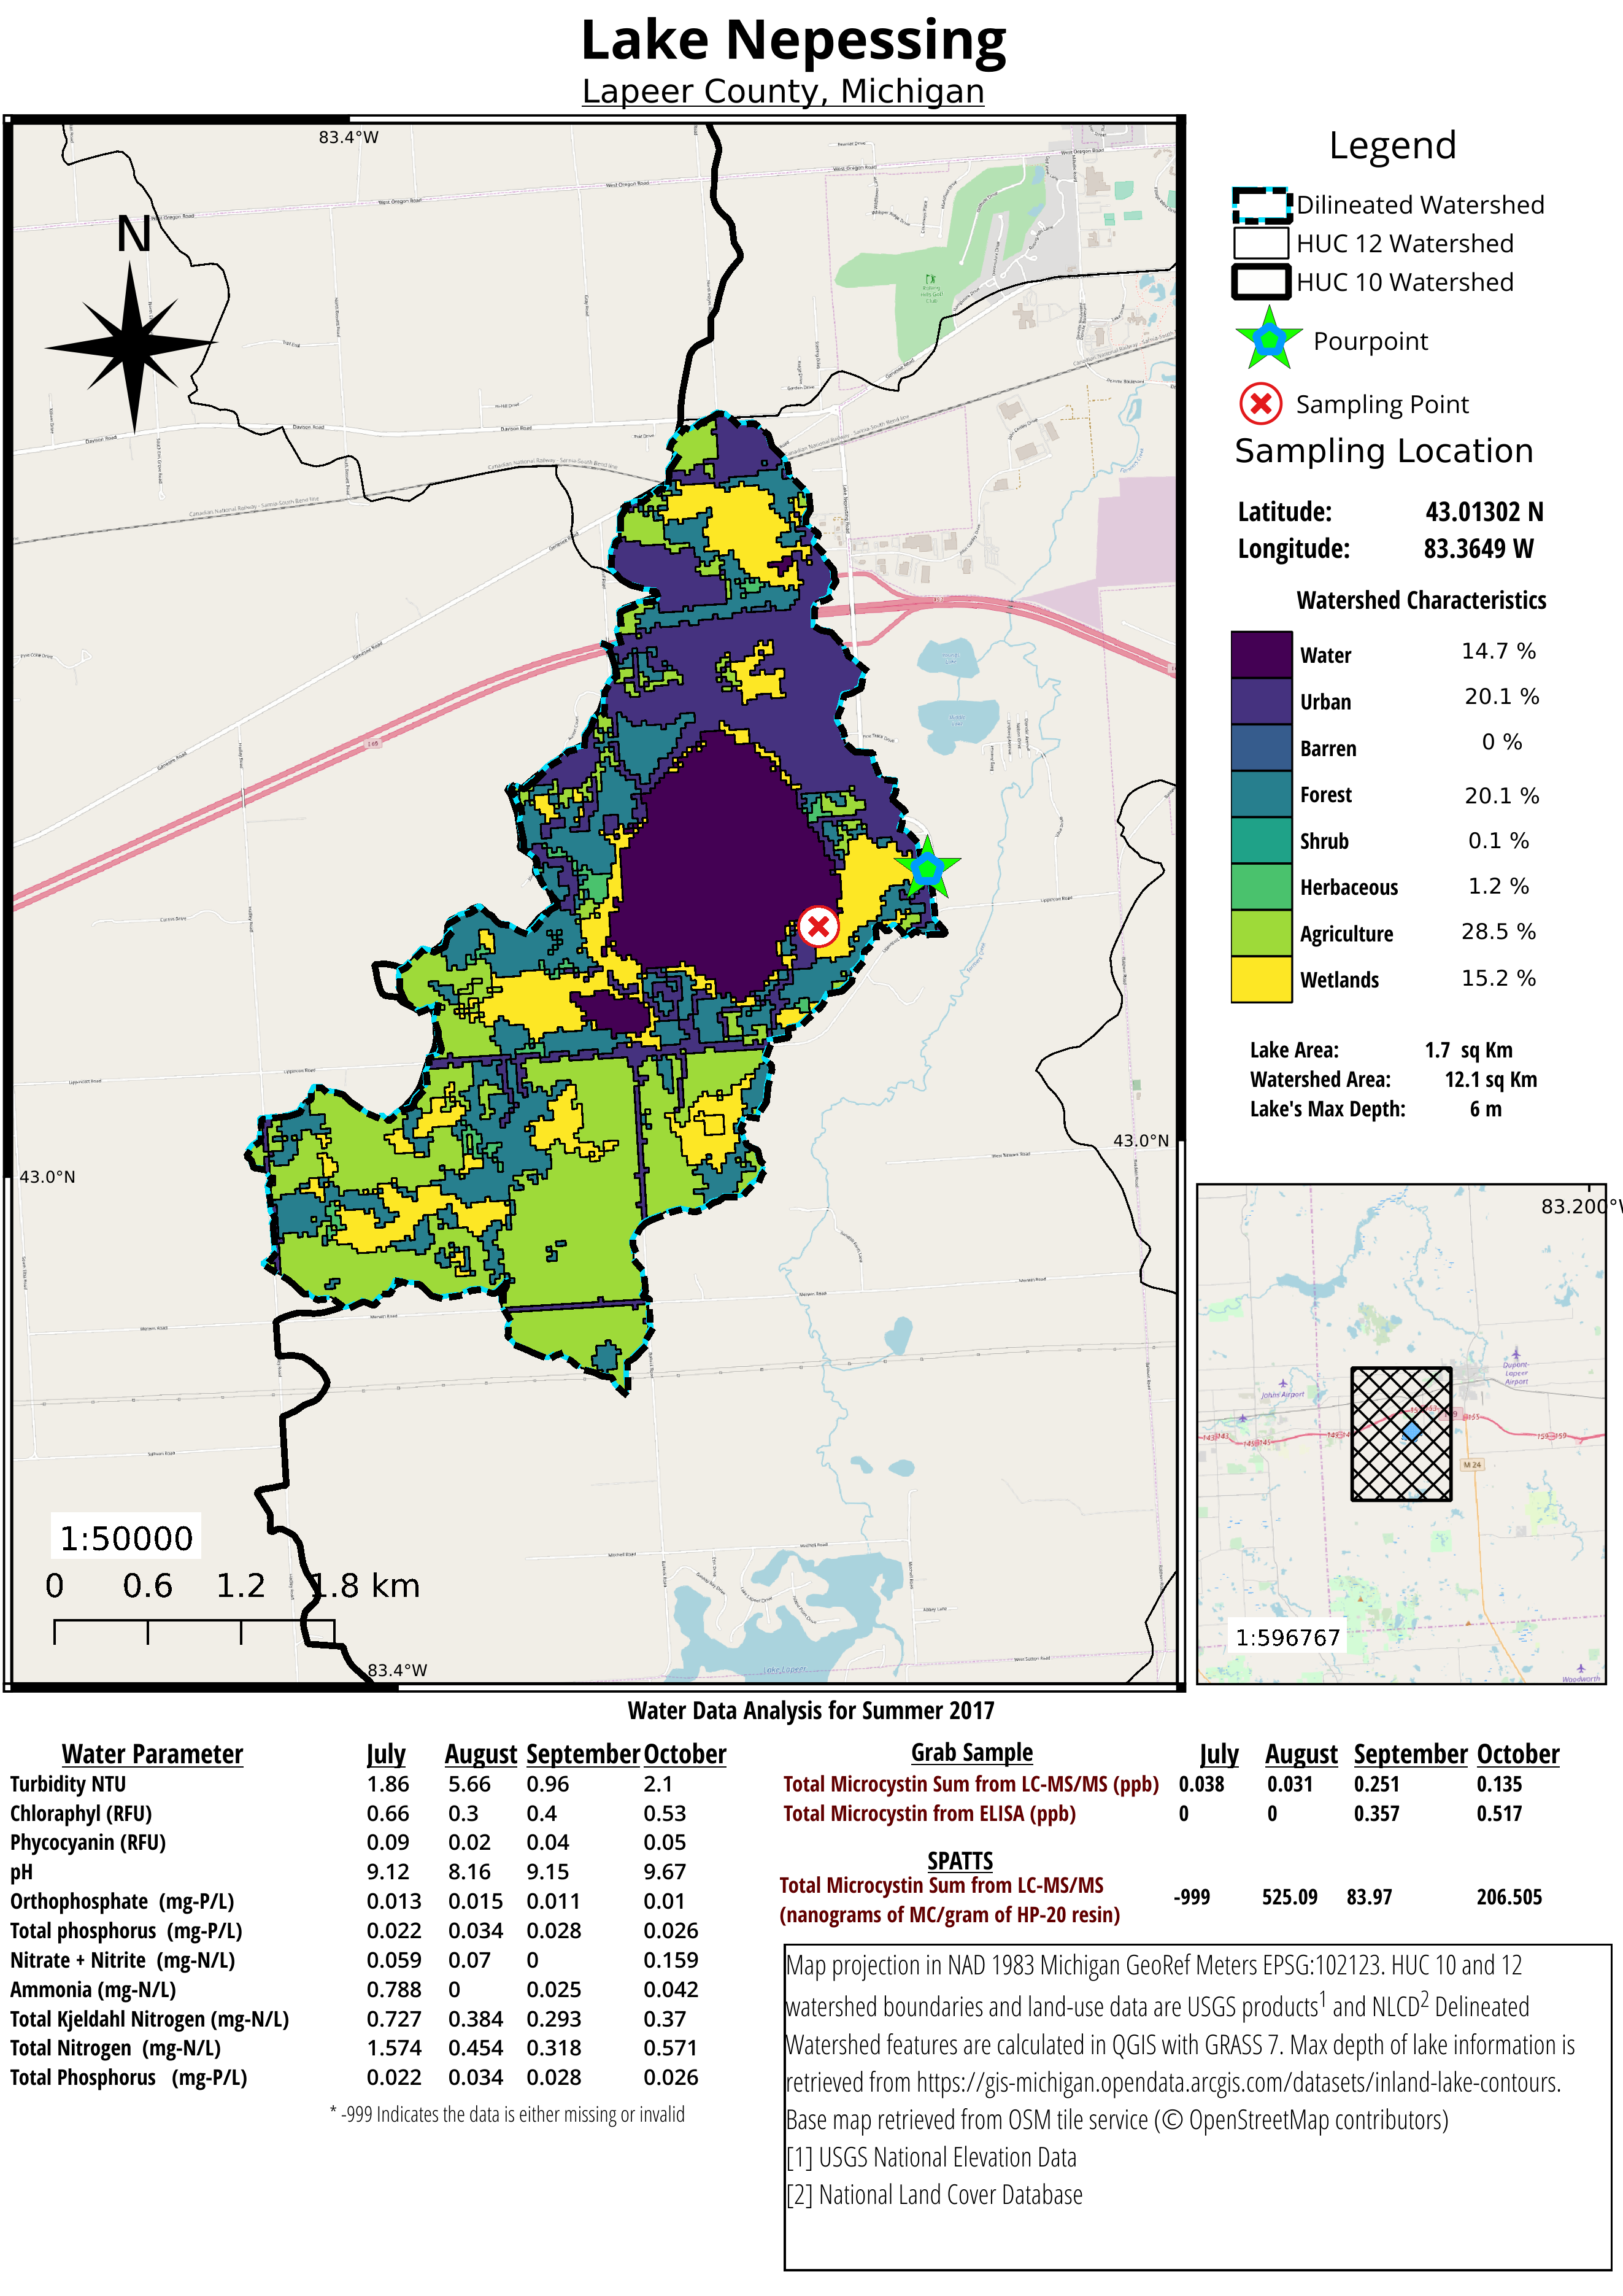
\includegraphics{figures/atlas/output_17}}
  }
\caption{GIS Map of Lake Nepessing}
\end{figure}

\begin{figure}[t]
\centerline{%
  \resizebox{\textwidth}{!}{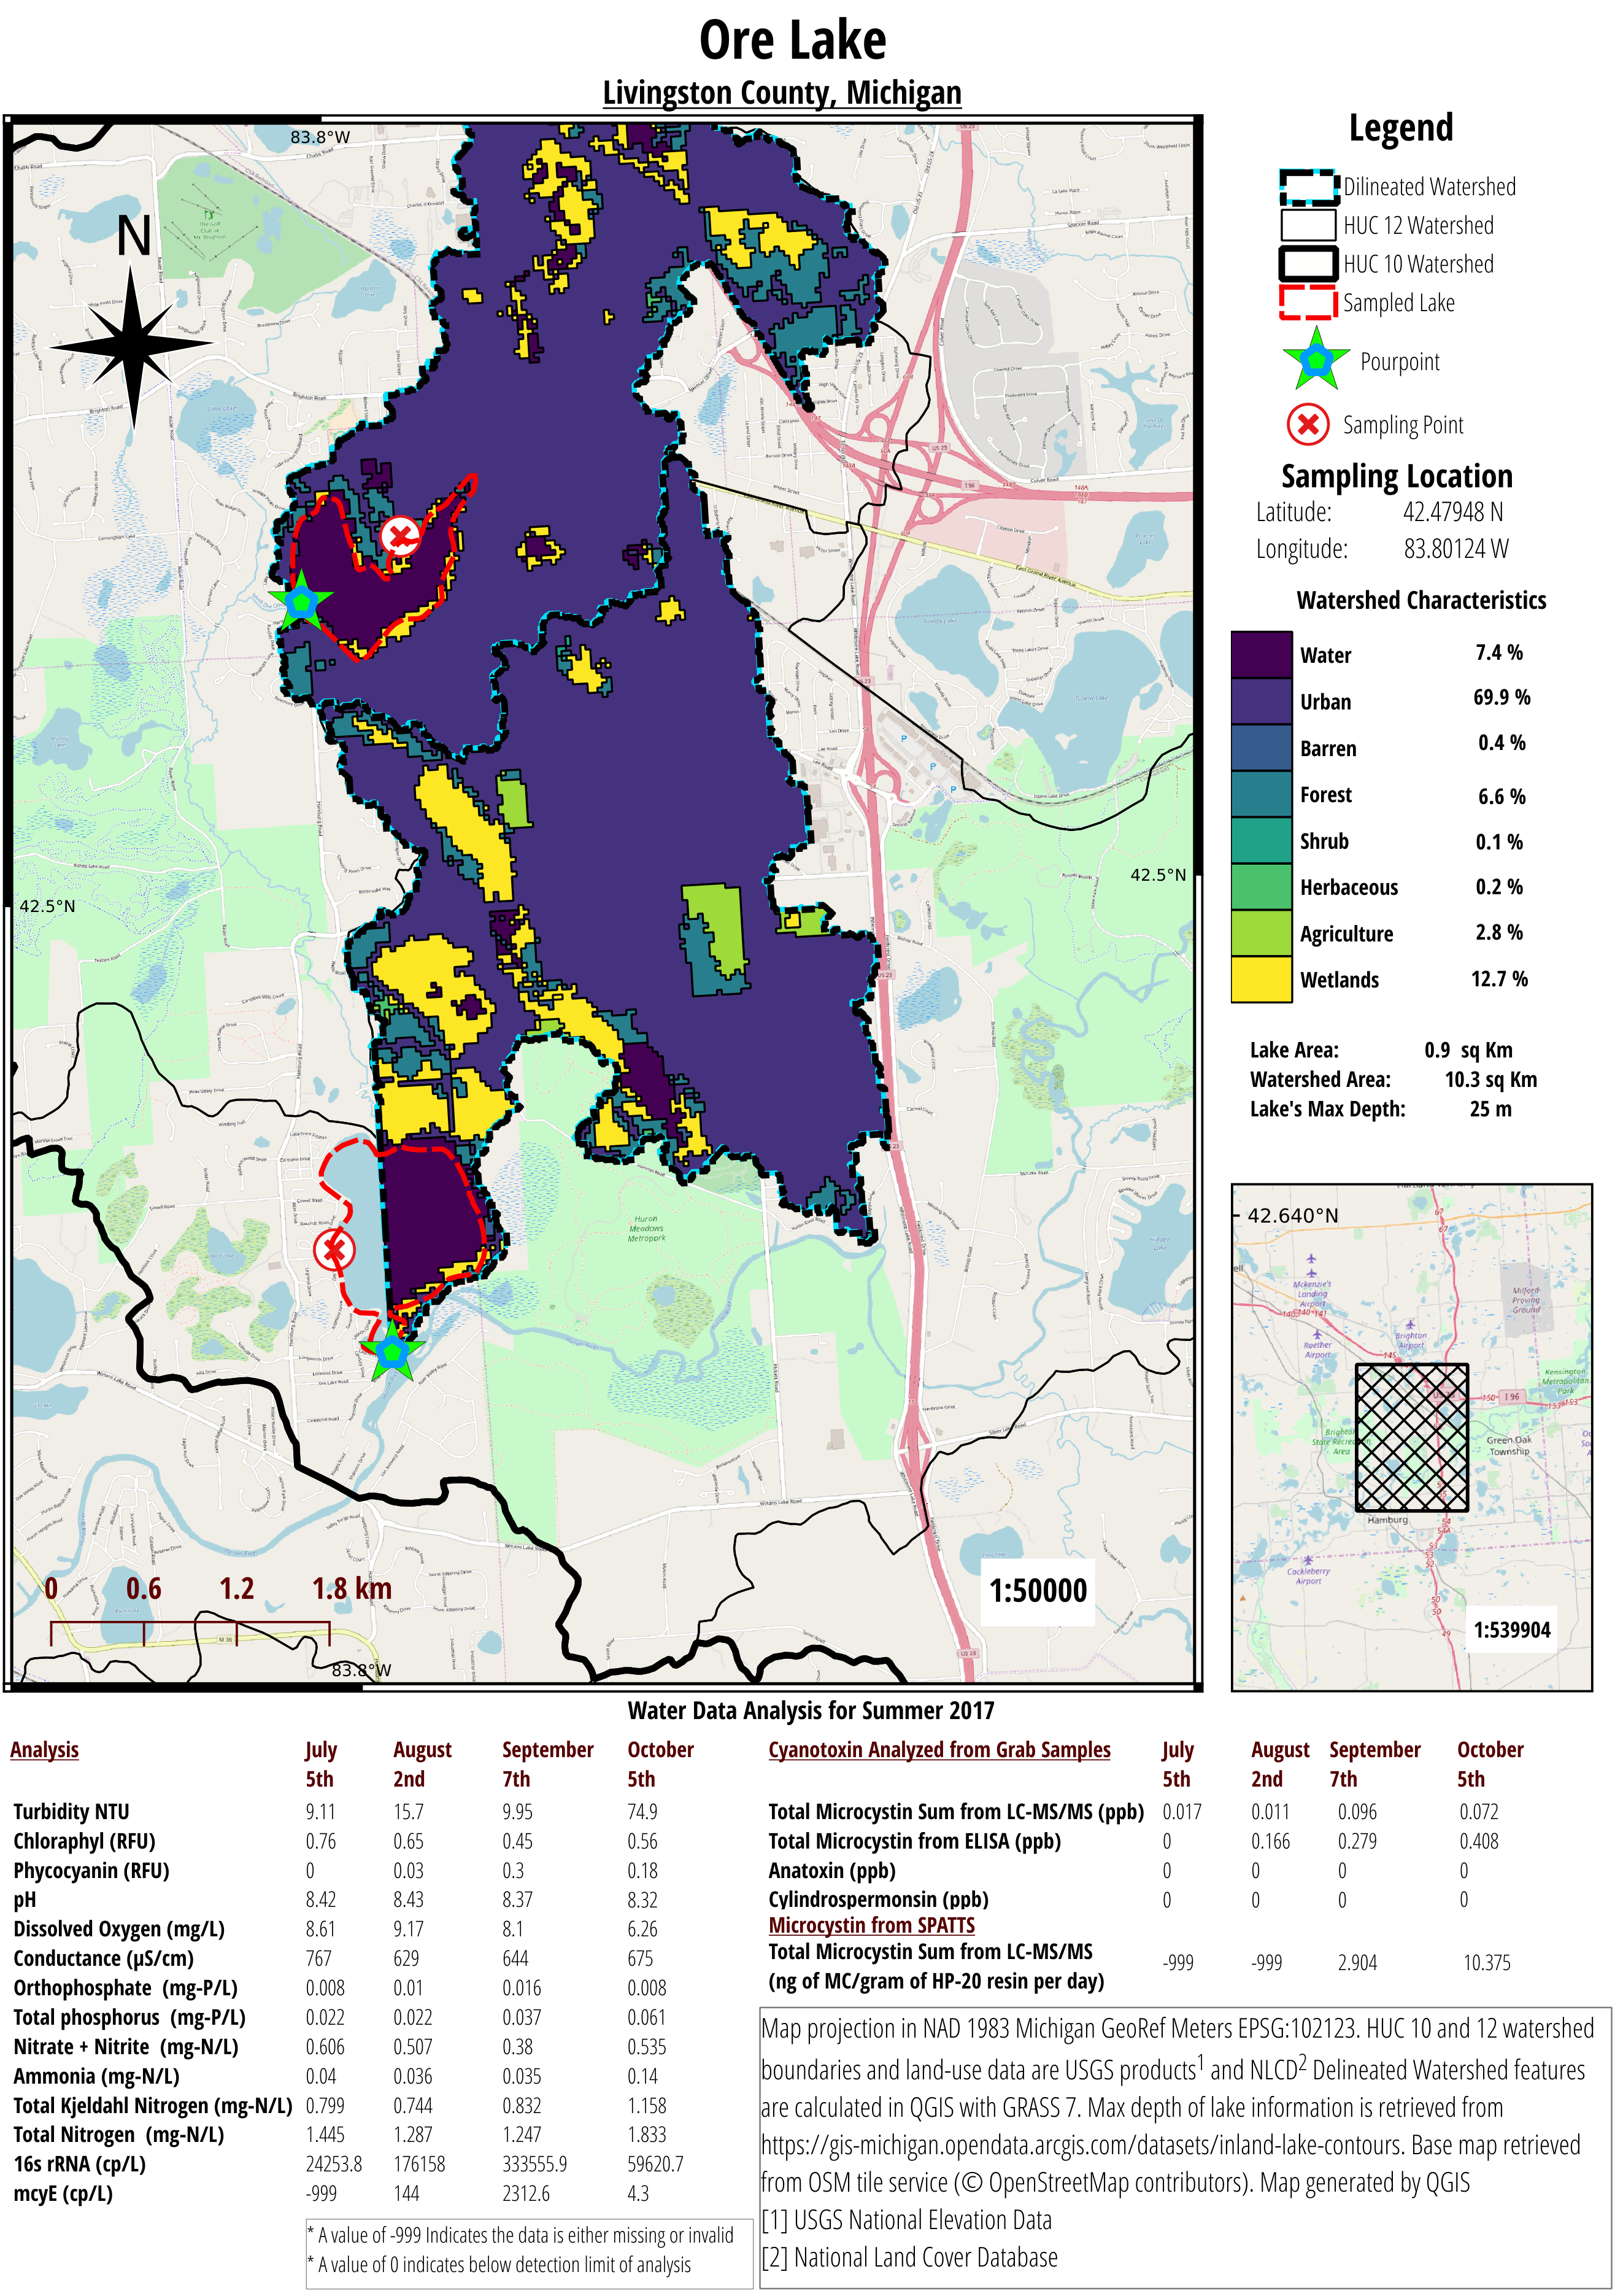
\includegraphics{figures/atlas/output_18}}
  }
\caption{GIS Map of Ore Lake}
\end{figure}

\begin{figure}[t]
\centerline{%
  \resizebox{\textwidth}{!}{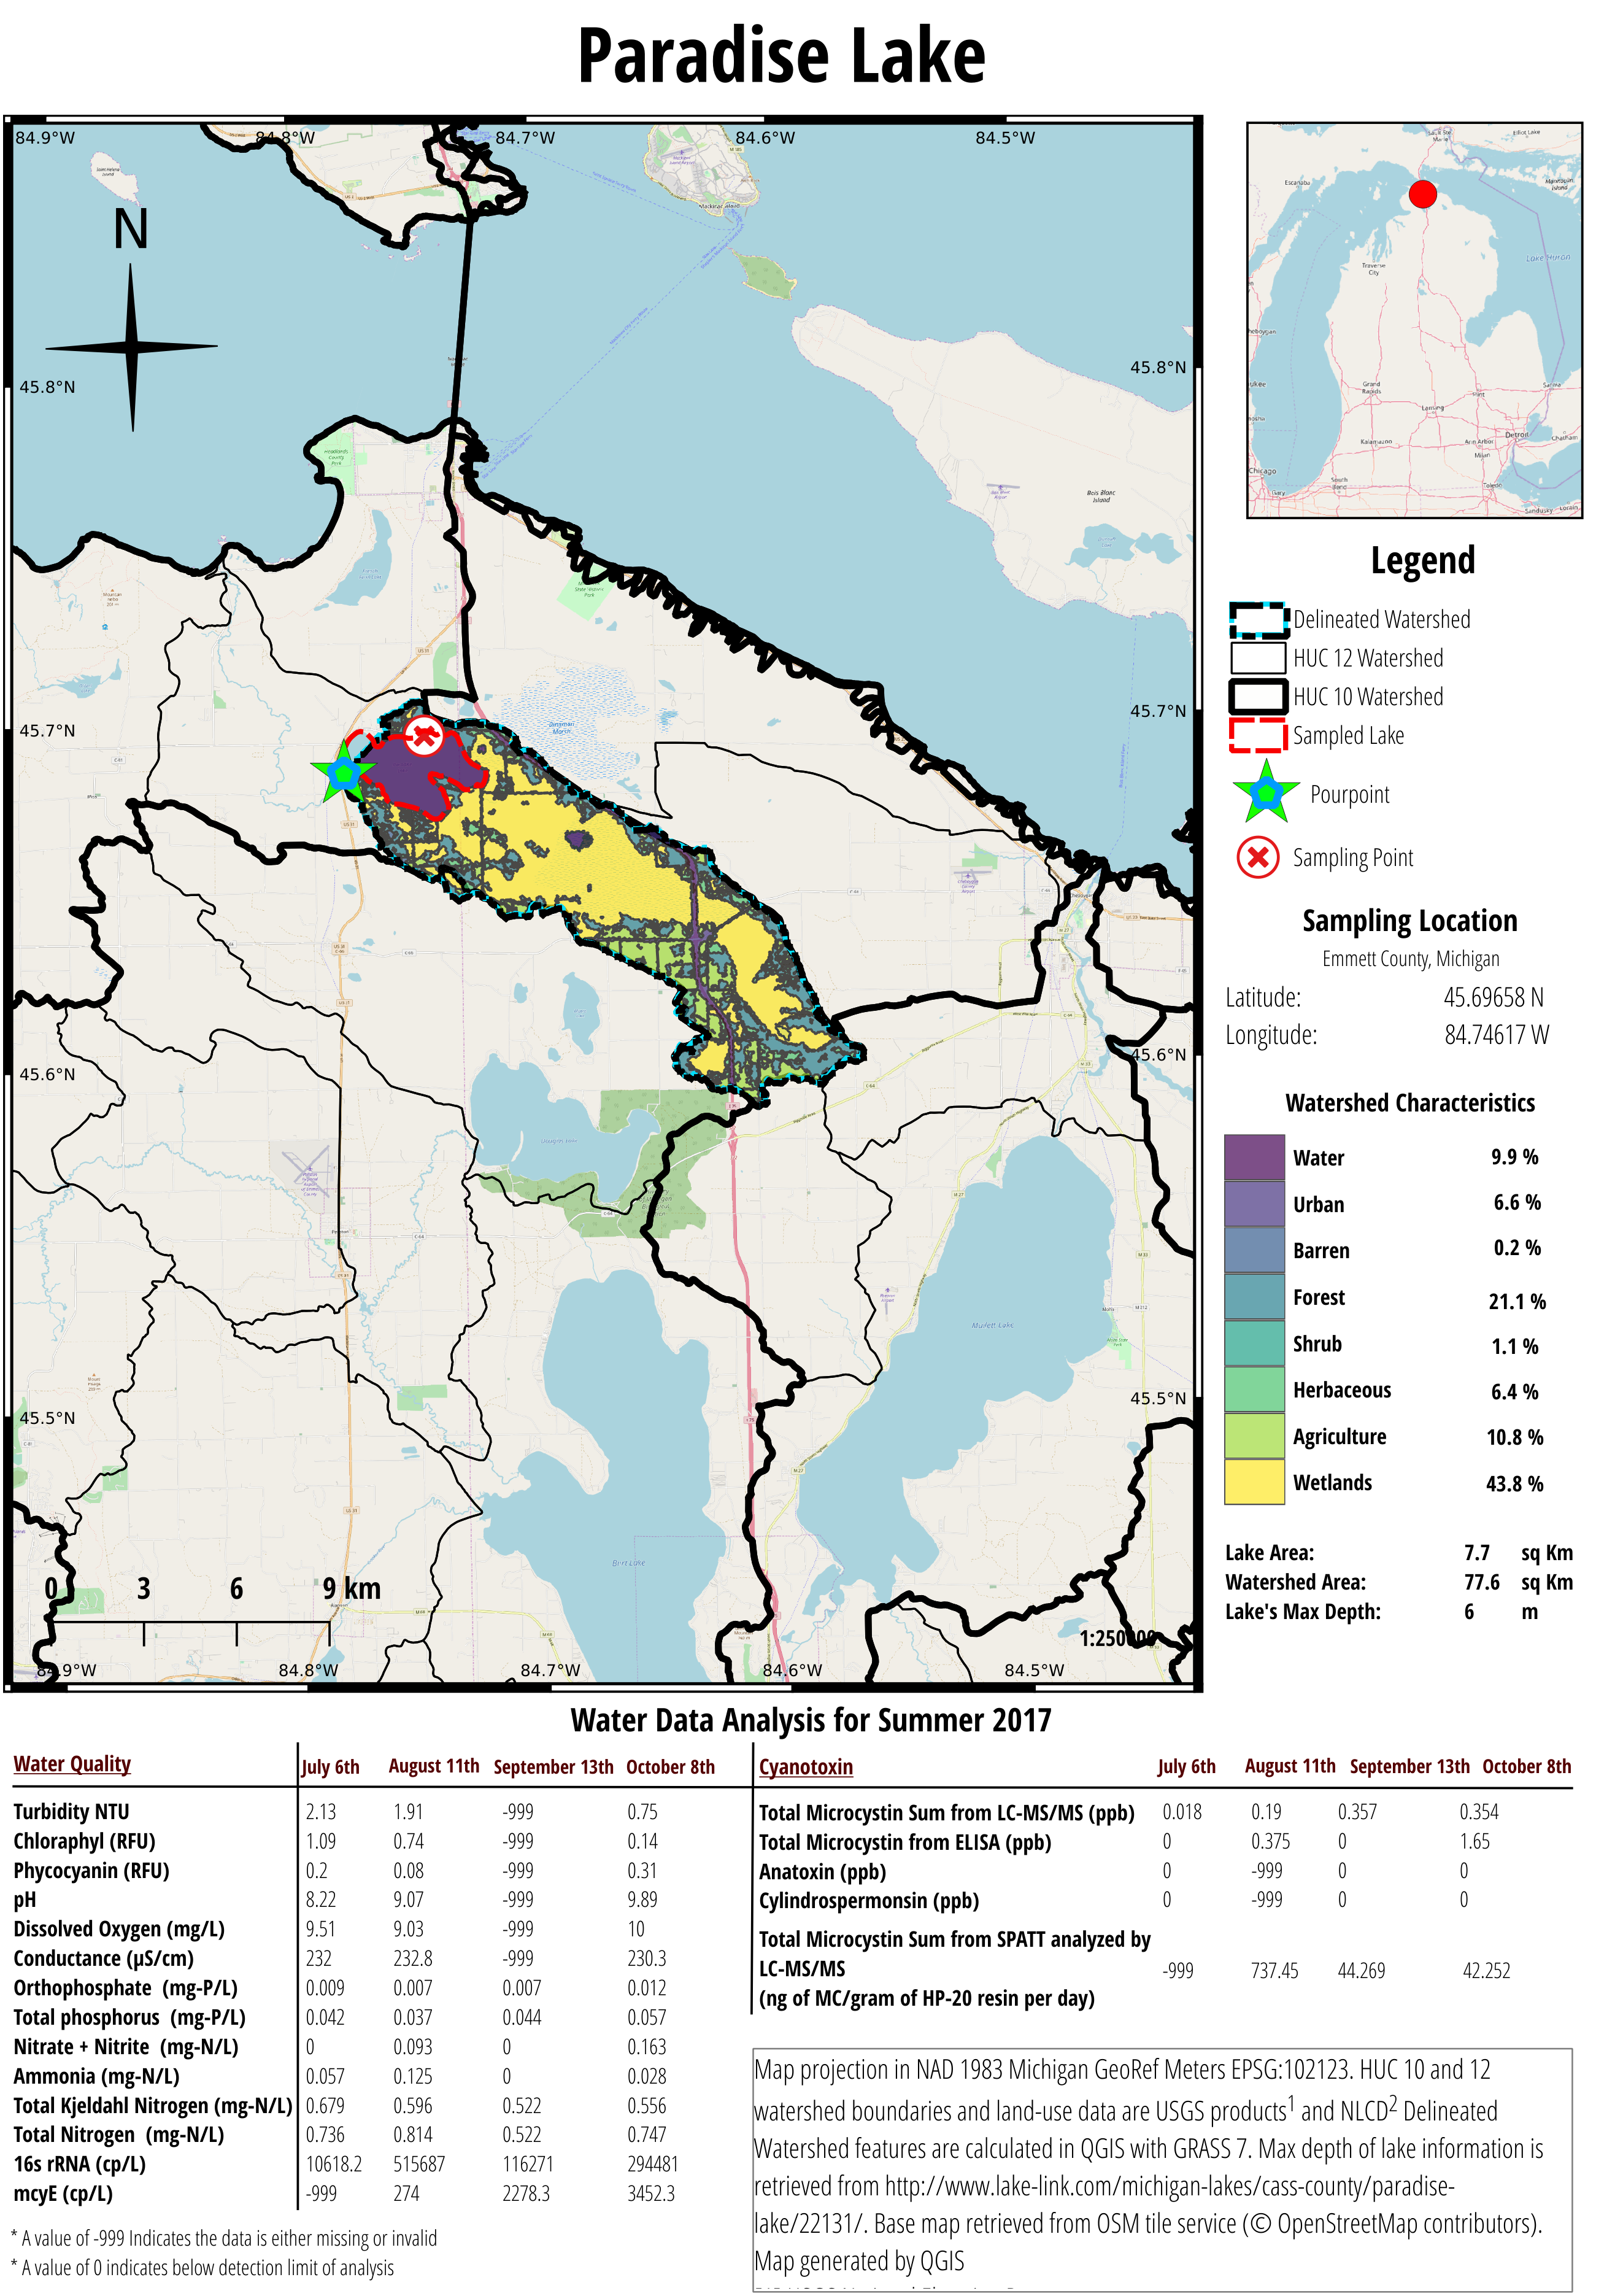
\includegraphics{figures/atlas/output_19}}
  }
\caption{GIS Map of Paradise Lake}
\end{figure}

\begin{figure}[t]
\centerline{%
  \resizebox{\textwidth}{!}{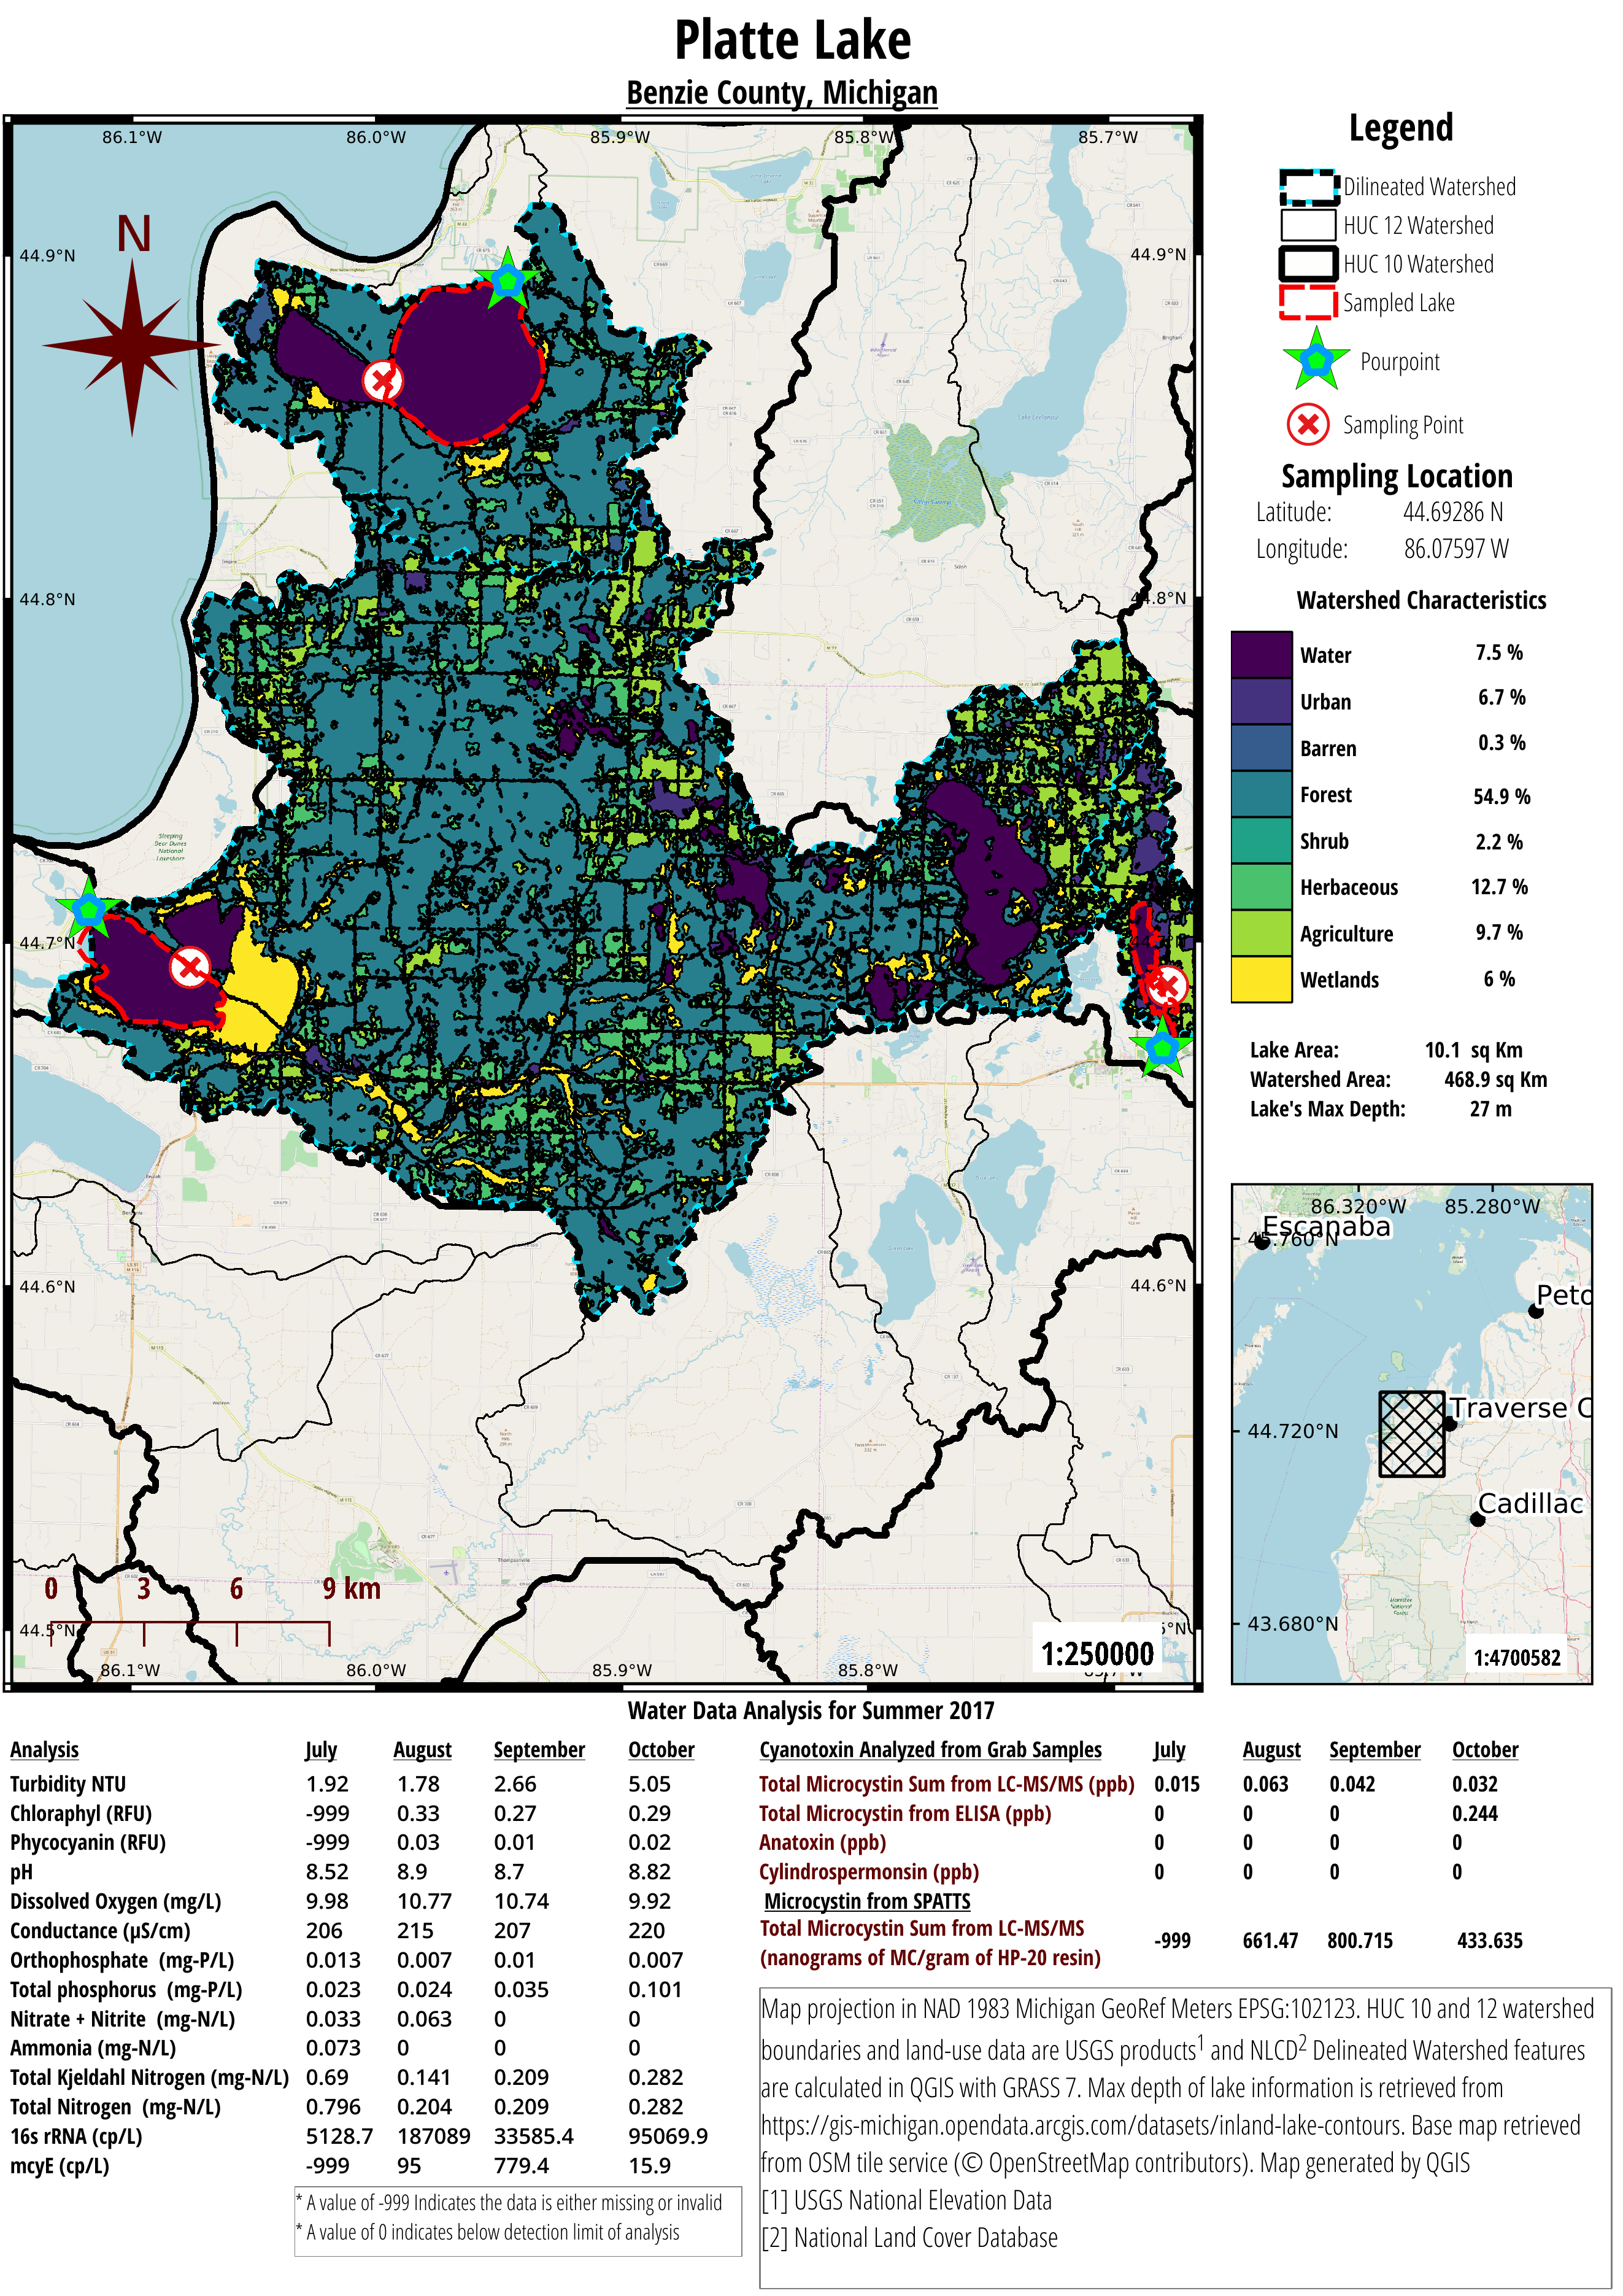
\includegraphics{figures/atlas/output_20}}
  }
\caption{GIS Map of Platte Lake}
\end{figure}

\begin{figure}[t]
\centerline{%
  \resizebox{\textwidth}{!}{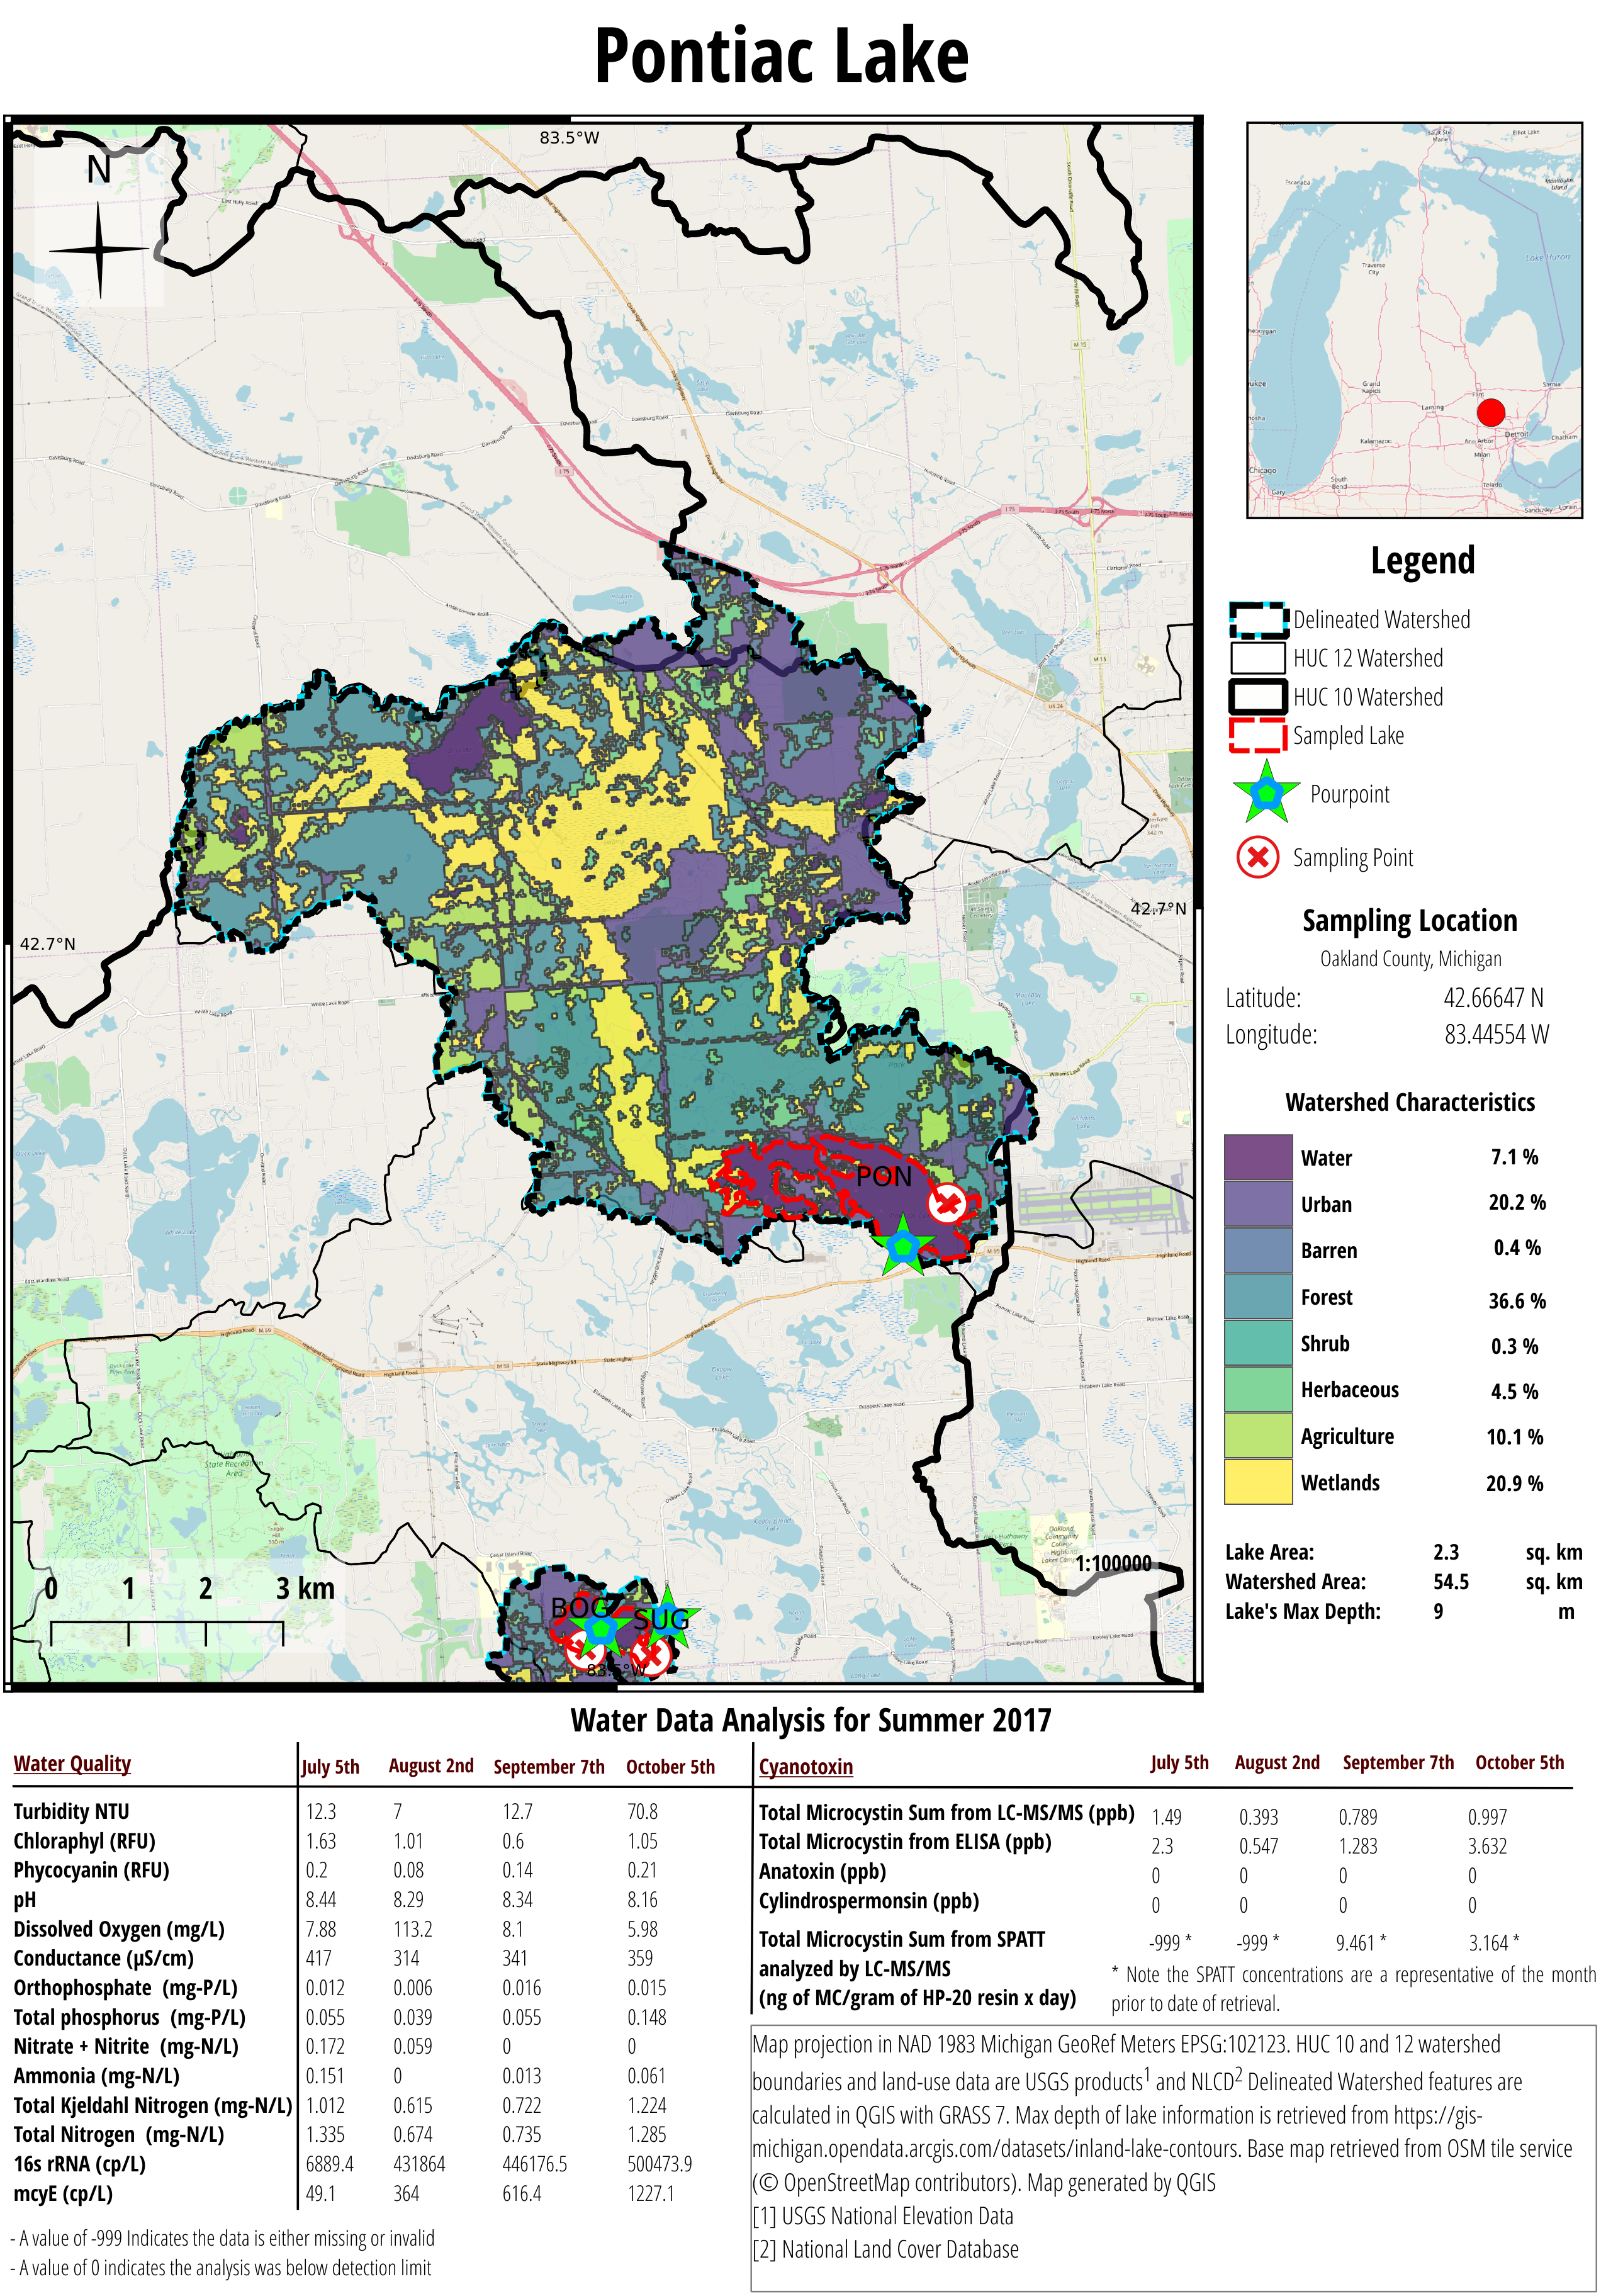
\includegraphics{figures/atlas/output_21}}
  }
\caption{GIS Map of Pontiac Lake}
\end{figure}

\begin{figure}[t]
\centerline{%
  \resizebox{\textwidth}{!}{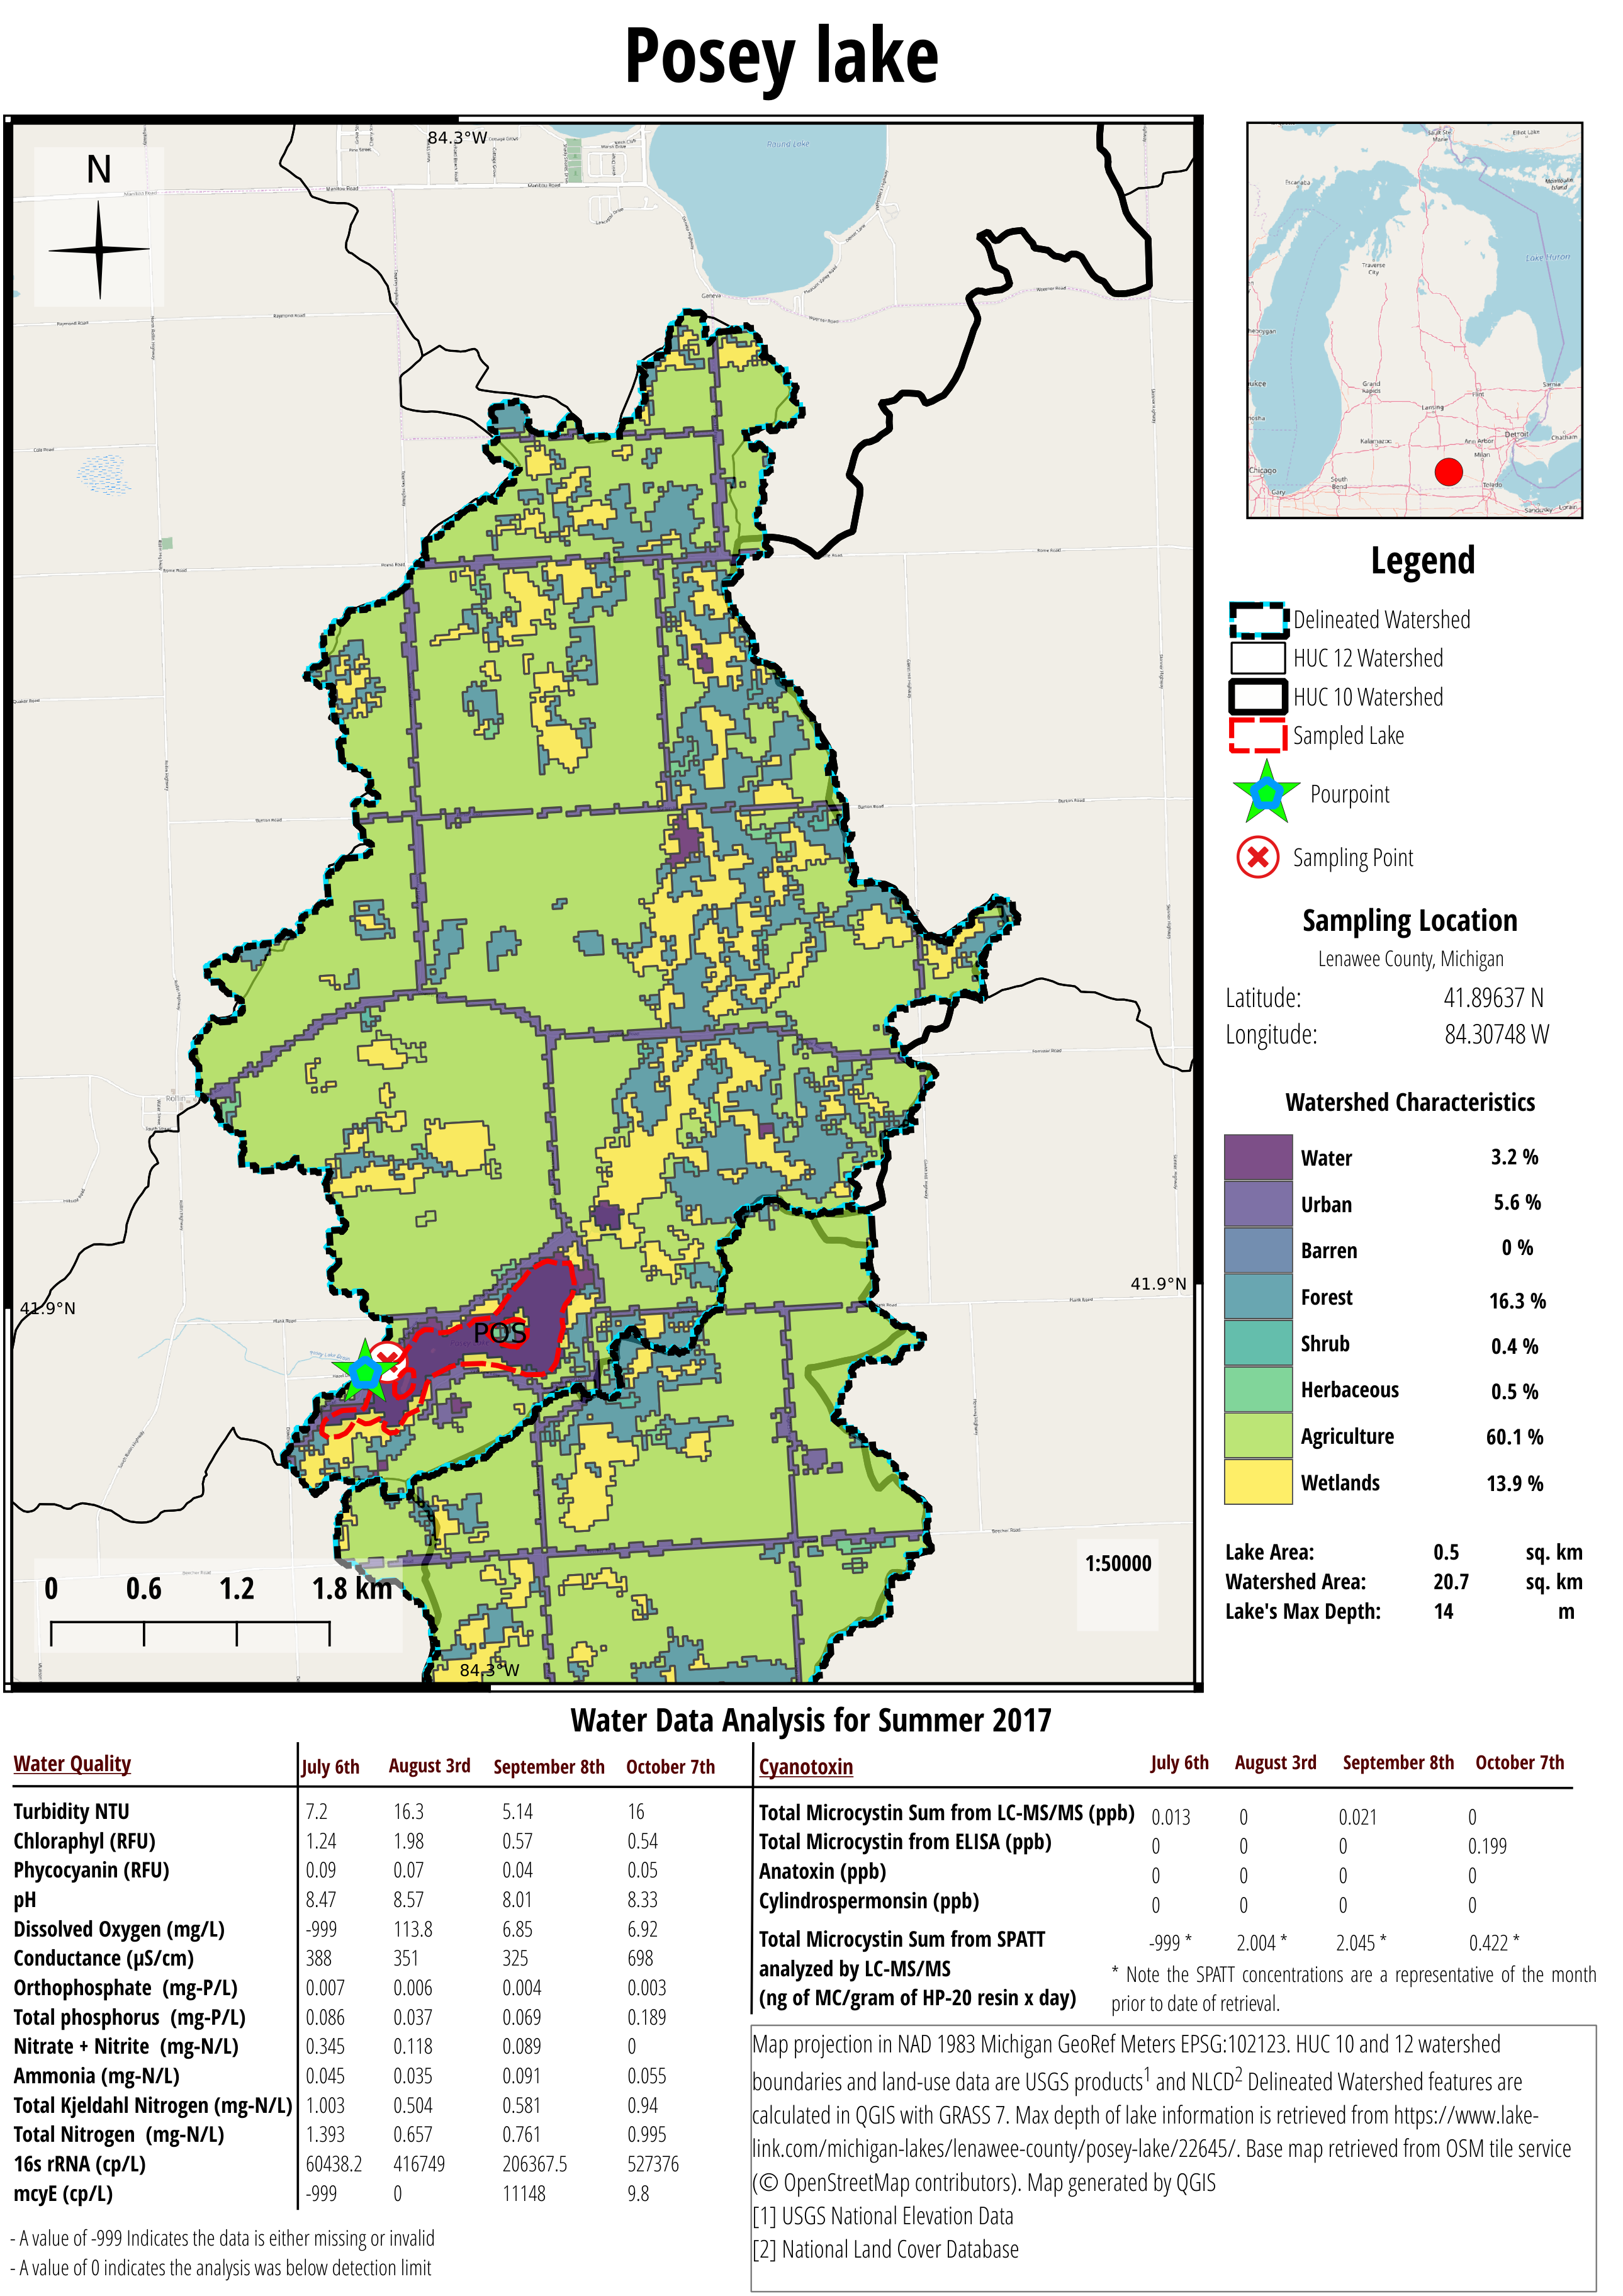
\includegraphics{figures/atlas/output_22}}
  }
\caption{GIS Map of Posey Lake}
\end{figure}

\begin{figure}[t]
\centerline{%
  \resizebox{\textwidth}{!}{\includegraphics{figures/atlas/output_23}}
  }
\caption{GIS Map of Round Lake}
\end{figure}

\begin{figure}[t]
\centerline{%
  \resizebox{\textwidth}{!}{\includegraphics{figures/atlas/output_24}}
  }
\caption{GIS Map of Sanford Lake}
\end{figure}

\begin{figure}[t]
\centerline{%
  \resizebox{\textwidth}{!}{\includegraphics{figures/atlas/output_25}}
  }
\caption{GIS Map of Silver Lake}
\end{figure}

\begin{figure}[t]
\centerline{%
  \resizebox{\textwidth}{!}{\includegraphics{figures/atlas/output_26}}
  }
\caption{GIS Map of Stoney Lake}
\end{figure}

\begin{figure}[t]
\centerline{%
  \resizebox{\textwidth}{!}{\includegraphics{figures/atlas/output_27}}
  }
\caption{GIS Map of Sugden Lake}
\end{figure}

\begin{figure}[t]
\centerline{%
  \resizebox{\textwidth}{!}{\includegraphics{figures/atlas/output_28}}
  }
\caption{GIS Map of Wixom Lake}
\end{figure}

\begin{figure}[t]
\centerline{%
  \resizebox{\textwidth}{!}{\includegraphics{figures/atlas/output_29}}
  }
\caption{GIS Map of West Twin Lake}
\end{figure}

\GrizzAppendix{Lake Atlas}


As a rough draft and to avoid pdf file to exceed size, 2 out of 29 lake maps are shown. In the final draft, all lake maps will be shown. All lake are the same format.

\clearpage
\newpage

\begin{figure}[t]
\centerline{%
  \resizebox{\textwidth}{!}{\includegraphics{figures/atlas/output_4}}
  }
\caption{GIS Map of Brighton Lake}
\end{figure}

\begin{figure}[t]
\centerline{%
  \resizebox{\textwidth}{!}{\includegraphics{figures/atlas/output_5}}
  }
\caption{GIS Map of Lake Cadillac}
\end{figure}

%\GrizzAppendix{Geospatial Data Collection Guide Using Open Data Kit}

\GrizzAppendixSection{Introduction}

Collaborative work is the fundamental part of a large scale research project.  Data aggregation and structural collection is one of the few key factors that determines the quality of the study. Large scale studies are often done by a team of multiple groups and organizations. There are available commercial tools which can aid in data collection and aggregation automatically. ArcGIS \footnote{ESRI 2017. ArcGIS Desktop: Release 10.5.1 Redlands, CA: Environmental Systems Research Institute.} coupled with their Android/IOS app called Collector for ArcGIS \footnote{https://www.esri.com/products/collector-for-arcgis}.

From my experience I found a viable alternative which does not require an expensive license. I wish to help other research studies with a cheaper alternative and greatly facilitate their pursuit. I have written this guide to allow anyone to build from the ground up on setting a database and providing a viable way to organize an enterprise. This guide is aimed to initially setup a database for non-profit organization and academic research with a limited budget. The initial cost is \$5 per month for a virtual private server (VPS) which has enough storage for a small database.  The software tool is from an open-source software by \gls{odk}\footnote{Open Data Kit 2.0: Expanding and Refining Information Services for Developing Regions \url{http://www.hotmobile.org/2013/papers/full/2.pdf} Waylon Brunette, Mitchell Sundt, Nicola Dell, Rohit Chaudhri, Nathan Breit, Gaetano Borriello In HotMobile, 2013. \url{http://dl.acm.org/citation.cfm?id=2444790}}.

\GrizzAppendixSection{Required Components}

Here you must setup a server that stores you data and be accessible through the Internet. Having your own computer machine as a server is a viable solution but it requires more extensive networking knowledge. An alternative solution is to purchase a rent a server from a third party which automatically sets up and quickly gets connected to the Internet. A Virtual Private Server (VPS) are cheap and flexible servers to set up a database up on the cloud. For as little as \$5 dollars a month one can have a server with everything they need to start collecting data.

DigitalOcean, Amazon (free trial for a year), Google VPS can work. I suggest anyone of them, but in this guide we will choose to setup from DigitalOcean as its the cheapest available server. I recommend Debian or Ubuntu linux distribution to setup your database. In this guide, we will choose Debian 9 (Stretch).

\GrizzAppendixSection{Syntax}
\noindent
In the terminal, you will need bash commands to setup the server's configuration. In this guide, bash commands will be represented the \$ symbol. Each line of code is represented with a single \$ at the beginning. Enter the text following anything after the \$. With some lines of code, there will be included comments which will be represented by the \#.

\begin{lstlisting}
  $ run this command   # This is a comment
\end{lstlisting}

\noindent
Note that the first line starts with a\#. This is not a command but a comment. In bash language, this is usually ignored. In this guide, a line starting with \$ designates a command. Do not include the \$ as its merely a symbol to designate a command. Running lines will not have \$ as its indented to be one line of code.

\GrizzAppendixSection{Server Setup}

\noindent
You must get an SSH client to access the server for setting up ODK Aggregate. For Linux or Mac, use the native terminal application to access the server. For windows users, I recommended program is PuTTy \url{https://www.putty.org/}. Install this program for windows. With PuTTy, open up PuTTy and enter in the IP address and click ``Open''. You will enter ``root'' and the password given by the online service or by the user installation setup.  Usually when using VPS services, the IP address and the password for user \emph{root} information is given by email.
\noindent
The command for linux or mac users, they can use Terminal and use this command:
\begin{lstlisting}[language=bash]
  $  ssh root@[EnterYourIp]   # SSH with root as user
  #  replace [EnterYourIp] with the given IP address
\end{lstlisting}

\noindent
From a fresh installation, the first prompt when accessing the server will be to change your password. Choose a good strong password for the root username and have it written down.  After setting the password, preform any upgrades and install sudo which allows a normal user to have elevated privileges and install nano, a text editor. This may be already installed but some distributions might not have them. To do this, follow these commands.

\begin{lstlisting}[language=bash]
  $  apt update            # Use the apt package manager and update repository
  $  apt upgrade -y        # Preform any upgrades
  $  apt dist-upgrade -y   # Distribution upgrades
  $  apt install sudo nano # Install the sudo and nano packages
\end{lstlisting}

\noindent
Next, we will set a separate username. The \emph{root} user is only used to administer the server.  Choose any name as you see fit and something you can remember. For our example, for the case of this guide, \emph{dummy} will be the username.

\begin{lstlisting}[language=bash]
  $  adduser dummy
\end{lstlisting}

\noindent
You will be prompted to create a password. When asked for name and other user information, hit ``Enter'' to leave it blank. This does not need to be filled out.

\noindent Here, we will also assign this new user as a sudo user. This will enable the new user to have elevated privileges. This will allow to run command lines with root access if ``sudo'' is run before the line of command. Be cautious with commands with sudo.

\begin{lstlisting}[language=bash]
  $  usermod -a -G sudo dummy # Add the user dummy to sudo group
\end{lstlisting}

\noindent
Its highly advisable to setup a pubic/private \gls{rsa} key pair for more secure login setup. This prevents unauthorized access to the server and prevents the basic brute-force attacks. Here are the steps necessary to secure the server against malicious attacks. We will also setup a firewall called ufw (Uncomplicated Firewall) which is very simple to setup and secure your server. We will also generate a key-pair for this user. You can have a passphrase which is an additional layer of security, or leave it blank. When generated, the public key will be located at \path{/home/dummy/.ssh/id_rsa.pub}. Follow this command:

\begin{lstlisting}[language=bash]
  $  su dummy             # Switch out from root and change the user to dummy
  $  sudo apt install ufw # Install uncomplicated firewall
  $  sudo ufw allow 22    # Allow SSH ports
  $  sudo ufw allow 8080  # Allow aggregate server
  $  sudo ufw allow 5432  # Allow PostgreSQL server
  $  ssh-keygen           # Generate the keys for SSH

\end{lstlisting}

\noindent
Next, we will move the generate public key to the authorized key folder. We will also limit the permissions of the authorized keys for only the user dummy to access, install putty tools and use it to convert the private key for windows client to use:

\begin{lstlisting}[language=bash]
  $  sudo mv ~/.ssh/id_rsa.pub ~/.ssh/authorized_keys
  $  chmod 600 ~/.ssh/authorized_keys
  $  sudo apt install putty-tools
  $  cd ~/.ssh
  $  puttygen id_rsa -o id_rsa.ppk

\end{lstlisting}

\noindent
Next, you have to retrieve the converted key file from the server to your own local machine. With windows, I recommend using WinSCP for secure file transfer \url{https://winscp.net/eng/index.php}. When prompted, enter the IP address in host name, port 22, and enter the new username and password (dummy). In WinSCP, hidden files are not shown by default. Hit Ctrl+Alt+H to show hidden files. On the right side panel, you will find the servers directory. The left side is the local computer's directory. Here we can transfer files between the machines securely. On the right side, locate .ssh folder and find the id\_rsa.ppk file and download it to your document folder. Simply double-click the file to download it to your local machine.

\noindent
This file can be pre-loaded int PuTTy. Double click the id\_rsa.ppk file, open up PuTTy and type the IP address. Entering in the username will automatically log in without password as the key authenticates you.

\noindent
Next, we will disable login by password which only allows users with the key file to access the server. This secures the server as it prevents malicious bots from brute-force attacks:

\begin{lstlisting}[language=bash]
  $  sudo nano /etc/ssh/sshd_config
\end{lstlisting}

\noindent
The command will open up \emph{nano} text editor. Scroll down the config file by pressing the down arrow key. Find the line that contains

\begin{lstlisting}
  >    PermitRootLogin yes
\end{lstlisting}

\noindent
Change it to:

\begin{lstlisting}[language=bash]
  >    PermitRootLogin no
\end{lstlisting}

\noindent
Scroll all the way to the end and find the line containing:

\begin{lstlisting}[language=bash]
  >    PasswordAuthentication yes
\end{lstlisting}

\noindent
And change it to:

\begin{lstlisting}[language=bash]
  >    PasswordAuthenticion no
\end{lstlisting}

\noindent
Make sure there is no \# in the beginning of the changed lines. Exit nano text editor by pressing ``Ctrl+X''. Press ``Y'' to save file and hit ``Enter'' to write file.

\noindent
Next restart ssh:

\begin{lstlisting}[language=bash]
  $  sudo service ssh restart
\end{lstlisting}

\noindent
Next, you will install ODK Aggregate. ODK Aggregate is a Java web applet that handles the data and stores into a database. The web applet is hosted as a website and can be accessed through any web browser. On the host machine, we will need to setup tomcat server that hosts ODK Aggregate along with an SQL server. PostgreSQL is used as we can also extend this to work with spatial data and be accessible from QGIS. As of writing this guide, ODK Aggregate is version 1.5.0. You may need to find the current version. Go to \url{https://github.com/opendatakit/aggregate}. If the version is different than 1.5.0, change the link following after the ``wget'' command.

\begin{lstlisting}
  $  sudo apt install tomcat8 unzip
  $  wget https://github.com/opendatakit/aggregate/releases/download/v1.5.0/ODK-Aggregate-v1.5.0-Linux-x64.run.zip
  $  unzip ODK-Aggregate-v1.5.0-Linux-x64.run.zip
  $  chmod +x ODK-Aggregate-v1.5.0-Linux-x64.run
  $  ./ODK-Aggregate-v1.5.0-Linux-x64.run
\end{lstlisting}

\noindent
You will see a prompt when the ODK Aggregate Setup Wizard appears. Follow these steps:

\begin{enumerate}
\item Read the license. Hit ``Enter'' to scroll through the document. Type ``Y'' at the end of the document to accept the license terms.
\item Type \path{ODK} to create a folder where the necessary files will be created.
\item  Type ``3'' to setup a PostgreSQL platform setup
\item Type ``Y'' to downloaded
\item Type ``N'' for ssl
\item Type ``1'' for no ssl
\item Type ``Y'' for port config
\item Hit ``Enter'' to default 8080
\item Type the IP address of the server.
\item Hit ``Y'' for PostgreSQL
\item Hit ``Enter'' to set the default PostgreSQL port to 5432
\item Hit ``Enter'' for default username \emph{odk\_user}
\item Make up a password for this user login
\item It will ask the name of the database \emph{odk\_prod}
\item Then it will ask to setup a name for your schema. \emph{odk\_prod}
\item The ``ODK Aggregate Instance Name'' is used as a display for your users. This can typically be set for a project name or title. For our purpose, it will be set to
\emph{demo}.
\item Create a super user name, most likely whomever is managing the data. We will set ours to be called \emph{super}.
\end{enumerate}

\noindent
Next, you must setup PostgreSQL:
\begin{lstlisting}
  $  echo deb http://apt.postgresql.org/pub/repos/apt/stretch-pgdg main | sudo tee -a /etc/apt/sources.list
  $  wget --quiet -O https://www.postgresql.org/media/keys/ACCC4CF8.asc | sudo apt-key add -
  $  sudo apt update
  $  sudo apt install postgresql-9.4
\end{lstlisting}

Next you need to create postgres as a username and setup a password. Here you will be switching into \emph{psql} command prompt to set things up. Once you are done, you will exit \emph{psql} by typing $\backslash$q which will lead into the regular bash home directory. Follow these command:

\begin{lstlisting}[language=bash]
  $  sudo -u postgres psql postgres #  This will log you into psql command prompt.
    % postgres=# \password postgres
    % postgres=# \q
  $                                 #  Back to bash command prompt
\end{lstlisting}

\noindent
Now you must set up the configuration of PostgreSQL to allow remote connections. You will edit the \path{/etc/postgreql/9.4/main/pg_hba.conf} file and the \path{/etc/postgresql/main/postgresql.conf}:

\begin{lstlisting}[language=bash]
  $  sudo nano /etc/postgresql/9.4/main/pg_hba.conf
\end{lstlisting}

\noindent
Change the line that has this:
\begin{lstlisting}[language=bash]
  >    local   all    all      peer
\end{lstlisting}
\noindent
To this:
\begin{lstlisting}[language=bash]
  >    local   all    all      md5
\end{lstlisting}

\noindent
Also add this line at the very end of the file:
\begin{lstlisting}[language=bash]
  >   host   all     all      0.0.0.0/0 md5
\end{lstlisting}

\noindent
Then exit by pressing ``Ctrl+X'', then hit ``Y'' to confirm, then hit ``Enter''. Lets edit the other file:

\begin{lstlisting}[language=bash]
  $  sudo nano /etc/postgresql/9.4/main/postgresql.conf
\end{lstlisting}

\noindent
Find this line:
\begin{lstlisting}[language=bash]
  >    #listen_addresses = 'localhost'
\end{lstlisting}

\noindent
Replace it with this, note the removal of  \# at the beginning of the line:

\begin{lstlisting}[language=bash]
  >    listen_addresses = '*'
\end{lstlisting}


\noindent
Now you will run the SQL configuration file generated from ODK Aggregate to setup the database in PostgreSQL. This will create the user \emph{odk\_user} and the database and schema \emph{odk\_prod}. Once this is done, you will restart PostgreSQL and have the database online.

\begin{lstlisting}[language=bash]
  $  sudo -u postgres psql postgres
      % postgres=# \cd '/home/dummy/ODK/ODK\ Aggregate'
      % postgres=# \i create_db_and_user.sql
      % postgres=# \q
  $  sudo systemctl restart postgresql
\end{lstlisting}


\noindent
ODK Aggregate run file from the previous step generated a .war file that needs to be copied to apache tomcat webapps folder. With tomcat8 installed on debian, the webapps folder is located at \path{/var/lib/tomcat8/webapps}.


\begin{lstlisting}[language=bash]
  $ cd $HOME/ODK/ODK\ Aggregate/
  $ sudo cp ODKAggregate.war /var/lib/tomcat8/webapps
  $ sudo service apache restart
\end{lstlisting}

\noindent
Now you should have the ODK Aggregate server running. You can simply access the server by going to your web browser on your local computer and access it by replacing your given ip address of the server in this form: \url{http://xxx.xxx.xxx.xxx:8080/ODKAggregate} Log into your super user login and click ``Site Admin''. Here you can add more users to administer the site or be a data collector. Site administrators have the ability to create more users and have all other power as a data collector. For a simple user who is just collecting data, you can have them set as ``Data Collector'' and not be able to change any data that has already been collected. Next, we must create a form for the data collectors to use.


\noindent
Before you start collecting data, you must set up a predefined form which consists of variables of interest. The ODK Collect app can collect spatial data in a form of GPS points, path of coordinates or trace a spatial polygon. ODK Aggregate can accept .xml files which needs to be created. The ODK Suite provides an online tool to create a desired form \url{https://build.opendatakit.org/}. When you first go to the site, you will be asked to sign up for a login. You do not have to create an account and can simply click cancel.

\noindent
Here you can design your survey form. On the top-right hand corner, you must name this form. This will be displayed for the user, so choose something that pertains to what kind of data is being collected. Next, you will choose what kind of data are going to be collected. The most important are usually the date/time and GPS coordinates. On the bottom, there is an option to select location. When selected, a configuration window will appear on your right-hand side. For the name, name it location. You can have it configured to be a single point, a path which creates a polyline, or a shape which creates a polygon shape. For the date and time, you can configure the full date and time or just the date. Depending on your project, you can select a variety of data ranging from audio or video data or a design questionnaire. For audio or video there is a media option. You can collect audio, video and picture or have all three options if you wish. The questionnaires can be designed by clicking the select multiple option. Here you can have options for the data collector to choose from. This can be configured to have a follow-up questions depending on what options the data collector initially selects. More information can be found by clicking help for more advance configurations.

\noindent
Once you have a satisfied form, you must save the form as an .xml file. On the top-right hand side, click File and select Export to XML. Once saved, head over you your ODK Aggregate website and click on ``Form Management''. Click ``Add New Form'' and select the .xml file to upload to the server.

\noindent
Next, the data collectors need to have the ODK Collect app to start collecting data. Android users can download the ODK Collect app either through the Google Play store or directly download the .apk file from \url{https://github.com/opendatakit/collect/releases/tag/v1.15.1}. Unfortunately there is no app for the IOS platform.

\noindent
First, you must set the settings. Go to the ``general settings'' and tap on ``server'' settings. For the option ``Type'' choose the \emph{ODK Aggregate} option. The URL will be the the same as the ODK Aggregate web address. Username and password will be the users that are created from ODK Aggregate website, or the super user. Head back to the main menu and click on ``Get Blank Form''. This will download the forms you have uploaded to the ODK Aggregate server. The app can collect data offline and send the filled forms once connected online. For each entry of data, tap the ``Fill Blank Form'' option and select the appropriate form. Here you will start filling out the form. Once completed, you will save the form offline. If you are connected to the Internet, you will have to upload the filled forms to the ODK Aggregate server. To do so, head to the main menu and select the ``Send Finalized Form'' option and simply tap on the form that is saved. This will now upload the data to your server.

\GrizzAppendixSection{Conclusion}

The utility from using ODK tools is beneficial for large scale studies, especially handing with geospatial data. ODK Aggregate is very flexible in working with other forms of applications. With PostgreSQL database, the stored data can be accessed either throught the ODK Aggregate webserver or by connecting to the PostgreSQL database connection. QGIS ,ArcGIS Desktop or Microsoft Access can connect to this database and pull data. For more advance configuration, see the ODK documentation: \url{https://docs.opendatakit.org/}. You may want to consider registering a domain name which allows you to enter a human-recognizable address instead of an IP address.

% References -- DO NOT EDIT
\phantomsection
\addcontentsline{toc}{chapter}{REFERENCES}
\singlespacing
\renewcommand{\bibname}{\vspace*{36pt}REFERENCES}
\bibliography{references}

\end{document}
